\documentclass[handout]{beamer}
\usepackage{standalone}

\input{slides-header.tex}

\title{Všechny prezentace z přednášek}
\subtitle{NAIL062 Výroková a predikátová logika}
\author{Jakub Bulín (KTIML MFF UK)}
% \institute{KTIML MFF UK}
\date{Zimní semestr 2024}

\begin{document}

\maketitle

\renewcommand{\maketitle}{}

\documentclass[handout]{beamer}
\usepackage{standalone}

\input{slides-header.tex}

\title{První přednáška (handout)}
\subtitle{NAIL062 Výroková a predikátová logika}
\author{Jakub Bulín (KTIML MFF UK)}
% \institute{KTIML MFF UK}
\date{Zimní semestr 2025}

\begin{document}

\documentclass{beamer}

\input{slides-header.tex}

\title{První přednáška}
\subtitle{NAIL062 Výroková a predikátová logika}
\author{Jakub Bulín (KTIML MFF UK)}
% \institute{KTIML MFF UK}
\date{Zimní semestr 2024}


\begin{document}


\maketitle


\begin{frame}{Jak se učit?}

    Velmi doporučuji tento online minikurz o efektivním učení:


    \href{https://www.samford.edu/departments/academic-success-center/how-to-study}{\alert{https://www.samford.edu/departments/academic-success-center/how-to-study}}

    Investujte 35 minut nyní, ušetřete mnoho hodin později!
    
\end{frame}


\begin{frame}{Cesta k jistému úspěchu u zkoušky}

    \begin{itemize}    
        \item \alert{Před přednáškou} alespoň zběžně projděte skripta, snažte se pochopit motivaci a smysl definic a hlavních tvrzení.
        \item Po přednášce skripta \alert{podrobně přečtěte}, nejasnosti ujasněte.
        \item Ujistěte se, že umíte pracovat i s \alert{formalizmem}.
        \item Věnujte pozornost i \alert{cvičení}, pomůže vám vše pochopit.
        \item Studujte \alert{průběžně}, a průběžně \alert{testujte své znalosti}.
    \end{itemize}

\end{frame}


\begin{frame}{První přednáška}

    \textbf{Program}
        \begin{itemize}
            \item úvod do logiky
            \item neformální představení výrokové a predikátové logiky (``upoutávka'')
            \item syntaxe výrokové logiky
            \item sémantika výrokové logiky (začátek)
        \end{itemize}

    \textbf{Materiály}

        \href{https://github.com/jbulin-mff-uk/nail062/raw/main/lecture/lecture-notes/lecture-notes.pdf}{\alert{\textbf{Zápisky z přednášky}}}, Kapitola 1 a Sekce 2.1-2.2.4 z Kapitoly 2

\end{frame}


\section{\sc Kapitola 1: Úvod do logiky}


\begin{frame}{Co je logika?}

    % \includegraphics[width=\textwidth]{slides1-images/definiton-of-logic.png}
    
    \href{https://www.google.com/search?q=define+logic}{\textbf{Dvě definice:}}
        \begin{enumerate}
            \item soubor principů, které jsou základem uspořádání prvků nějakého systému (např. programu, zařízení, protokolu)
            \item věda o uvažování prováděném podle striktních pravidel zachovávajících platnost 
        \end{enumerate}
        
    \medskip 
    
    \pause

    \myblock{\textbf{V informatice obojí:} daný systém nejprve \emph{formálně popíšeme}, a poté o něm \emph{formálně uvažujeme} (automaticky!), tj. odvozujeme \alert{platné inference} za použití nějakého \alert{dokazovacího systému}
    }

\end{frame}


\begin{frame}{Historie a aplikace logiky}

    {\footnotesize Filozofie $\to$}  {\normalsize Matematika $\to$}  {\Large Teoretická informatika $\to$} 
    
    \medskip
    
    \myalertinline{\Huge Aplikovaná informatika}

    \pause

    \medskip

    \begin{itemize}
        \item logic programming
        \item discrete optimization (SAT solving, scheduling, planning)
        \item database theory
        \item verification (software, hardware, protocol)
        \item automated reasoning and proving
        \item knowledge-based representation
        \item artificial intelligence
    \end{itemize}

\end{frame}


\section{1.1 Výroková logika}


\begin{frame}{Příklad ze života: Hledání pokladu}

    \myexample{
        Při hledání pokladu jsme narazili na rozcestí dvou chodeb. Víme, že na konci každé chodby je buď poklad, nebo drak, ale ne obojí. 
        
        \pause

        \medskip
        Trpaslík nám řekl, že: 
        \begin{itemize}
            \item \emph{``Alespoň jedna z těch dvou chodeb vede k pokladu''}, a že
            \item \emph{``První chodba vede k drakovi.''}
        \end{itemize}

        \pause

        \medskip
        Je známo, že trpaslíci buď vždy mluví pravdu, nebo vždy lžou. Kterou cestou se máme vydat?
    }

\end{frame}


\begin{frame}{Výroky neformálně}

    \alert{Výrok} je tvrzení, kterému lze přiřadit pravdivostní hodnotu: 
    \begin{center}
        \alert{pravdivý} (\emph{True}, 1), nebo \alert{lživý} (\emph{False}, 0)
    \end{center}

    \pause
    
    \alert{Prvovýroky} (\alert{atomické výroky}, \alert{výrokové proměnné}) zkombinované pomocí logických spojek a závorek do \alert{složených výroků}:

    \pause

    \myexample{
        ``(Trpaslík lže,) \emph{právě když} (druhá chodba vede k drakovi.)''\
    }
    
    \medskip

    \pause

    \begin{description}\setlength{\itemsep}{3pt}
        \item[\LARGE\alert{$\neg$}] ``neplatí X'', \emph{negace}
        \item[\LARGE\alert{$\landsymb$}] ``X a Y'', \emph{konjunkce}
        \item[\LARGE\alert{$\lorsymb$}] ``X nebo Y'', \emph{disjunkce} (není exkluzivní)
        \item[\LARGE\alert{$\limpliessymb$}] ``pokud X, potom Y'', \emph{implikace} (čistě logická)
        \item[\LARGE\alert{$\liffsymb$}] ``X, právě když Y'', \emph{ekvivalence}
    \end{description}

\end{frame}


\begin{frame}{Formalizace ve výrokové logice}

    Volba množiny prvovýroků: \myalertinline{bity informace popisující daný systém}

    \pause
    
    \myexample{            
        $p_1=${\it ``Poklad je v první chodbě.''}\\
        $p_2=${\it ``Poklad je ve druhé chodbě.''}
    }

    \pause

    (Co nejmenší, např. hodnota $t=${\it ``Trpaslík mluví pravdu.''} je jednoznačně určená hodnotami $\mathbb P=\{p_1,p_2\}$.)
    
    \pause

    \begin{itemize}
        \item {\it Poklad nebo drak, ale ne obojí}: zakódované do volby $\mathbb P$ (přítomnost draka je absence pokladu)
        \item {\it ``První chodba vede k drakovi.''} $\Leftrightarrow$ \alert{$\neg p_1$}
        \item {\it ``Alespoň jedna z chodeb vede k pokladu.''} $\Leftrightarrow$ \alert{$p_1 \lor p_2$}
        \item {\it Trpaslík buď mluví pravdu, nebo lže}:
        \myexamplemath{
        $$
        \varphi = (\neg p_1 \land (p_1 \lor p_2)) \lor (\neg (\neg p_1) \land \neg (p_1 \lor p_2))
        $$
        }
    \end{itemize}

    \pause

    \medskip
    \myblock{
    \alert{Teorie} $T=\{ \varphi \}$ v \alert{jazyce} $\mathbb P=\{p_1,p_2\}$, $\varphi$ je \alert{axiom} $T$.
    }

\end{frame}


\begin{frame}{Modely a důsledky}

    Lze určit, kde je poklad? Je $p_1$ nebo $p_2$ \alert{důsledkem} $\varphi$ resp. $T$?    

    \alert{``Svět''}, ve kterém je např. v první chodbě poklad a ve druhé drak, popíšeme pomocí \alert{pravdivostního ohodnocení} $p_1=1,p_2=0$, neboli \alert{modelu} $v=(1,0)$ jazyka $\mathbb P$. Celkem máme 4 ``světy'' a modely:
    \myexample{\vspace{-6pt}
    $$
    \M_\mathbb P=\{(0,0),(0,1),(1,0),(1,1)\}.
    $$
    }

    \pause

    Je ``svět'' popsaný modelem $v = (1,0)$ \emph{konzistentní} s tím, co víme, tj. \alert{platí} v modelu $v$ výrok $\varphi$ resp. teorie $T$? Vyhodnotíme podle stromové struktury $\varphi$:
    $$
    v(p_1) = 1,\ v(p_2) = 0,\ v(\neg p_1) = 0,\ v(p_1 \lor p_2)=1,\ \dots,\ \alert{v(\varphi)=0}
    $$
    
    \pause

    Množina \alert{modelů výroku} \( \varphi \) (resp.\ \emph{modelů teorie} \( T \)):
    \myexample{\vspace{-6pt}
    $$
    \M_\mathbb P(\varphi)=\M_\mathbb P(T)=\{(0,1)\}.
    $$
    }

    \myblock{V \alert{každém modelu} teorie $T$ platí výrok $p_2$, neboli $p_2$ je \alert{důsledek}~$T$.}
    
\end{frame}


\begin{frame}{Dokazovací systémy}

    Ověřovat všechny modely je nepraktické, pro $|\mathbb P|=n$ máme $2^n$ modelů, a $\mathbb P$ může být i nekonečná.

    \pause

    \textbf{Dokazovací systém}
    \begin{itemize}
        \item \alert{důkaz} výroku~\( \psi \) z teorie \(T\) je formálně definovaný syntaktický objekt, snadno (mechanicky) ověřitelný
        \item lze hledat algoritmicky čistě na základě struktury \( \psi \) a axiomů \(T\) (``\emph{syntaxe}''), nemusíme se zabývat modely (``\emph{sémantikou}'').
    \end{itemize}        
    
    \pause
    Klíčové vlastnosti:

    \pause
    \myblock{
    \begin{itemize}
        \item \alert{korektnost}: pokud existuje důkaz \( \psi \) z \(T\), potom \( \psi \) platí v \(T\)
        \item \alert{úplnost}, pokud \( \psi \) platí v \(T\), potom existuje důkaz \( \psi \) z \(T\)
    \end{itemize}
    }

    \pause
    %Korektnost je nutná, ale efektivní dokazovací systém může být užitečný, i pokud v něm nelze dokázat vše, co platí.
    Ukážeme si \alert{metodu analytického tabla} a \alert{rezoluční metodu}. Obě dokazují \emph{sporem}: předpokládají platnost $T$ a \( \neg \psi \), hledají spor.

\end{frame}


\begin{frame}{Metoda analytického tabla}

\begin{itemize}
    \item důkaz je strom olabelovaný předpoklady o platnosti výroků
    \item v kořeni: \alert{neplatí} dokazovaný výrok $\psi$ (důkaz sporem)
    \item připojíme platnost axiomů z $T$
    
    \pause
    \item při konstrukci zjednodušujeme výroky ve vrcholech, \alert{invariant}:
    
    \pause
    \bigskip
    \myalert{\it
        Každý model teorie \(T\), ve kterém neplatí \(\psi\), se musí \emph{shodovat} s některou z větví tabla. 
    }

    \pause
    
    \bigskip

    např.:
    
    \bigskip
    \myblock{
    \alert{\small True $(\varphi_1 \limplies \varphi_2 )$} zredukujeme rozvětvením na \alert{\small False $\varphi_1$} a \alert{\small True $\varphi_2$},\\
    \alert{\small False $(\varphi_1 \limplies \varphi_2 )$} zredukujeme připojením \alert{\small True $\varphi_1$} a \alert{\small False $\varphi_2$}.
    }
    \smallskip    
        
    \pause

    \item \alert{sporná} větev = předpokládá True i False stejného výroku
    \item \alert{důkaz} = všechny větve sporné (tj. nemůže existovat model $T$, ve kterém neplatí $\psi$)
\end{itemize}

\end{frame}


\begin{frame}{Příklad tablo důkazu}

    \vspace{-6pt}
    \begin{figure}\scalebox{0.8}{\small
        \centering
        \begin{forest}
        [False \( p_2 \)
            [True \( (\neg p_1 \land (p_1 \lor p_2)) \lor (\neg (\neg p_1) \land \neg (p_1 \lor p_2)) \) 
                [True \( \neg p_1 \land (p_1 \lor p_2) \)
                    [True \( \neg p_1 \)
                        [True \( p_1 \lor p_2 \)
                            [False \( p_1 \)
                                [True \( p_1 \), tikz={\node[fit to=tree,label=below:\alert{fail}] {};}
                                ]
                                [True \( p_2 \), tikz={\node[fit to=tree,label=below:\alert{fail}] {};}
                                ]
                            ]
                        ]
                    ]
                ]
                [True \( \neg (\neg p_1) \land \neg (p_1 \lor p_2) \)
                    [True \( \neg (\neg p_1) \)
                        [True \(\neg (p_1 \lor p_2) \)
                            [False \( (\neg p_1) \)
                                [True \( p_1 \)
                                    [False \(p_1 \lor p_2 \)
                                        [False \(p_1\)
                                            [False \(p_2\), tikz={\node[fit to=tree,label=below:\alert{fail}] {};}
                                            ]
                                        ]
                                    ]
                                ]
                            ]
                        ]
                    ]
                ]
            ]
        ]
        \end{forest}

    }
    \end{figure}    

\end{frame}


\begin{frame}{Konjunktivní normální forma (CNF)}

    \alert{literál} $p$, $\neg p$\hfill \alert{klauzule} disjunkce literálů\hfill \alert{CNF} konjunkce klauzulí

    \myblock{
        každý výrok má \alert{ekvivalentní} CNF (\alert{$\psi \sim \psi'$}, stejné modely)
    }
    
    \pause
    \myexample{např. pro výrok 
    $
    (\neg p_1 \land (p_1 \lor p_2)) \lor (\neg (\neg p_1) \land \neg (p_1 \lor p_2))
    $
    }

    \pause
    nahradíme \alert{$\neg (\neg p_1) \sim p_1$} a \alert{$\neg (p_1 \lor p_2) \sim (\neg p_1 \land \neg p_2)$} (\emph{De Morgan})

    \pause
    \myexamplemath{
    $$
    (\neg p_1 \land (p_1 \lor p_2)) \lor (p_1 \land \neg p_1 \land \neg p_2)
    $$
    }

    \pause
    a dále opakovaně použijeme \alert{distributivitu} \( \lorsymb \) vůči \( \landsymb \): \medskip

    \pause
    \myexampleamsmath{
    \begin{gather*}
    (\neg p_1 \lor p_1) \land (\neg p_1 \lor \neg p_1) \land (\neg p_1 \lor \neg p_2) \land (p_1 \lor p_2 \lor p_1) \land\\ (p_1 \lor p_2 \lor \neg p_1)\land (p_1 \lor p_2 \lor \neg p_2)    
    \end{gather*}    
    }

    \pause
    už je CNF, ještě zjednodušíme: odstraníme duplicitní literály, a klauzule obsahující $p_i$ a zároveň $\neg p_i$ (to jsou \alert{tautologie})

    \pause
    \myexamplemath{
    $$
    \neg p_1 \land (\neg p_1 \lor \neg p_2) \land (p_1 \lor p_2)
    $$
    }

\end{frame}


\begin{frame}{Rezoluční důkaz}

    Dk sporem, převeď \alert{negaci} dokazovaného do CNF a přidej k $T$

    \pause
    \myblock{
    \alert{\(p_2\) platí v \(T\)}, právě když je následující CNF výrok \alert{nesplnitelný}:
    }

    \myexamplemath{
    $$
    \neg p_1 \land (\neg p_1 \lor \neg p_2) \land (p_1 \lor p_2)\land\alert{\neg p_2}
    $$
    }

    \pause
    množinový zápis:
    \myexampleinline{$
    S=\left \{ \{\neg p_1\},\{\neg p_1,\neg p_2\},\{p_1, p_2\},\{\neg p_2\} \right \}
    $
    }

    \pause
    \medskip

    \myalert{\alert{rezoluční pravidlo}: je-li $p\in C_1$ a $\neg p\in C_2$, potom \emph{rezolventa} 
    $$
    C= (C_1\setminus \{p\})\cup(C_2\setminus \{\neg p\})
    $$ platí v každém modelu, ve kterém platí $C_1$ i $C_2$
    }
    
    \pause
    \medskip

    \alert{rezoluční zamítnutí $S$}: posloupnost klauzulí, kde každá je buď z $S$ nebo rezolventa předchozích, poslední je prázdná klauzule $\square$

    \pause
    \myblock{\textbf{myšlenka:} protože $\square$ nemá žádný model, je i $S$ nesplnitelná}

\end{frame}


\begin{frame}{Příklad rezolučního důkazu}

    \alert{rezoluční zamítnutí} (3. klauzule je rezolventou 1.\&2., 5. je z 3.\&4.)

    \myexamplemath{
    \[
        \{\neg p_1\},\{p_1, p_2\},\{p_2\},\{\neg p_2\},\square
    \]
    }

    \pause
    \bigskip

    \alert{rezoluční strom} (listy klauzule z $S$, vnitřní vrcholy rezolventy synů) 

    \myexample{
        \begin{center}
            \begin{forest}
            for tree={grow=north}
            [\( \square \)
                [\( \{\neg p_2\} \)]
                [\( \{p_2\} \)
                [{\( \{p_1, p_2\} \)}]
                [\( \{\neg p_1\} \)]
                ]
            ]
            \end{forest}
        \end{center}
    }

\end{frame}


\begin{frame}{Příklad: Barvení grafů}

    \myexample{
    Najděte vrcholové obarvení následujícího grafu třemi barvami.
    \begin{center}
    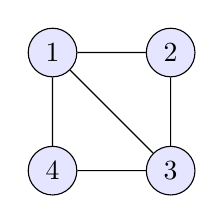
\begin{tikzpicture}[every node/.style={circle,fill=blue!10,draw,minimum size=0.5cm,node distance=1.5cm}]
    \node (1) {$1$};
    \node[right of=1] (2) {$2$};
    \node[below of=2] (3) {$3$};
    \node[left of=3] (4) {$4$};
    \path[draw] (1) -- (2) -- (3) -- (4) -- (1) -- (3);
    \end{tikzpicture}
    \end{center}
    }
    
    \pause
    graf: množina vrcholů a množina (libovolně) \alert{orientovaných} hran
    \[
    \mystructure G = \langle V; E \rangle = \langle \{1,2,3,4\}; \{(1,2),(1,3),(1,4),(2,3),(3,4)\} \rangle
    \]
    \pause
    jak formalizovat? pro $v\in V$ a $c\in C=\{R,G,B\}$:
    
    \myalertmath{
    $$
    p_v^c=\text{\it``vrchol \(v\) má barvu \(c\)''}
    $$
    }

    \pause
    \mbox{\small $\mathbb P=\{p_v^c\mid c\in C,v\in V\}=\{p_1^R,p_1^G,p_1^B,p_2^R,p_2^G,p_2^B,p_3^R,p_3^G,p_3^B,p_4^R,p_4^G,p_4^B\}$}

    \pause
    máme celkem \( |\M_\mathbb P|=2^{12}=4096 \) \alert{modelů jazyka} (12-dim. vektorů)
\end{frame}


\begin{frame}{Formalizace hranového obarvení}

    \begin{itemize}
        \item každý vrchol má nejvýše jednu barvu: $4^4=2^8=256$ modelů\medskip

        \myexamplemath{\vspace{-9pt}$$
        T_1 = \{ (\neg p_v^R \lor \neg p_v^G) \land (\neg p_v^R \lor \neg p_v^B) \land (\neg p_v^G \lor \neg p_v^B) \mid v \in V \}
        $$}

        \pause
        \medskip

        \item a každý vrchol má alespoň jednu barvu: $3^4=81$ modelů\medskip
        
        \myexamplemath{\vspace{-9pt}$$T_2 = T_1\cup \{ p_v^R \lor p_v^G \lor p_v^B \mid v \in V \}= T_1\cup \{\bigvee_{c\in C} p_v^c \mid v \in V \}
        $$}

        \pause
        \medskip
        
        \myblock{$T_2$ je \alert{extenze} teorie $T_1$ neboť \alert{každý důsledek $T_1$ platí i v $T_2$}, zde dokonce $\M_\mathbb P(T_2)\subseteq\M_\mathbb P(T_1)$}
        %\footnote{Proč $\subseteq$? Čím více vlastností požadujeme, tím méně objektů je splňuje.}

        \pause
        \medskip

        \item nakonec přidáme \alert{hranovou podmínku}:\medskip
        
        \myexamplemath{$$
        T_3 = T_2\cup \{ \bigwedge_{c\in C} 
        (\neg p_u^c \lor \neg p_v^c) \mid (u,v) \in E \}
        $$}  

        \pause
        \medskip

        Výsledná teorie \( T_3 \) je \alert{splnitelná} (má model), právě když je graf \( \mystructure{G} \) 3-obarvitelný.   
    \end{itemize}

\end{frame}


\begin{frame}{Co s ní?}

\textbf{Všechna obarvení?} 

$T_3$ má 6 modelů: \( v = (1,0,0,0,1,0,0,0,1,0,1,0) \) a další získané permutací barev \vspace{-12pt}
\begin{center}
    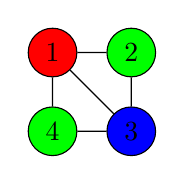
\begin{tikzpicture}[every node/.style={circle,fill=blue!10,draw,minimum size=0.3cm,node distance=1cm}]
    \node[fill=red] (1) {$1$};
    \node[fill=green,right of=1] (2) {$2$};
    \node[fill=blue,below of=2] (3) {$3$};
    \node[fill=green,left of=3] (4) {$4$};
    \path[draw] (1) -- (2) -- (3) -- (4) -- (1) -- (3);
    \end{tikzpicture}
\end{center}

\pause

\textbf{Obarvení, ve kterých je vrchol 1 modrý a vrchol 2 zelený?} 

Odpovídají modelům teorie \( T_3 \cup \{ p_1^B, p_2^G\} \)

\pause

\textbf{Důkaz, že vrcholy 2 a 4 musí mít stejnou barvu?}

\alert{Tablo} s kořenem $\text{False  }(p_2^R \land p_4^R)\lor(p_2^G \land p_4^G)\lor(p_2^B \land p_4^B)$

\pause

Nebo \alert{rezolucí}: přidáme \alert{negaci} \( (p_2^R \land p_4^R)\lor(p_2^G \land p_4^G)\lor(p_2^B \land p_4^B) \), vše převedeme do CNF a zamítneme

\end{frame}


\section{1.2 Predikátová logika}


\begin{frame}{Nevýhody formalizace ve výrokové logice}
Teorie $T_3$ je poměrně velká, a `natvrdo' kóduje graf $\mystructure G$.

\pause

\begin{center}
    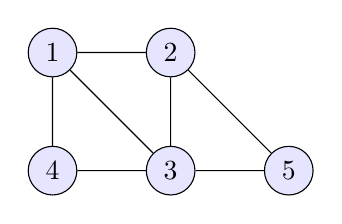
\begin{tikzpicture}[every node/.style={circle,fill=blue!10,draw,minimum size=0.5cm,node distance=1.5cm}]
    \node (1) {$1$};
    \node[right of=1] (2) {$2$};
    \node[below of=2] (3) {$3$};
    \node[left of=3] (4) {$4$};
    \path[draw] (1) -- (2) -- (3) -- (4) -- (1) -- (3);
    \node[right of=3] (5) {$5$};
    \path[draw] (2) -- (5) -- (3);
    \end{tikzpicture}
\end{center}

\pause
Obohatit jazyk $\mathbb P'=\mathbb P \cup \{ p_5^R,p_5^G,p_5^B\}
$ a vytvořit ještě větší teorii~$T'_3$ přidáním axiomů o vrcholu 5 a hranách $(2, 5), (3,5)$?

\pause
A co vlastnosti obecně platné o všech nebo mnoha grafech?

\pause
\myblock{
V \alert{predikátové logice} můžeme mluvit \alert{o vrcholech} grafu pomocí \alert{proměnných} a přirozeně vyjádřit vlastnosti jako:
\begin{itemize}
    \item \emph{``z vrcholu \(u\) vede hrana do vrcholu \(v\)''}
    \item \emph{``vrchol \(u\) je zelený''}
\end{itemize}
}
\end{frame}


\begin{frame}{Predikátová logika: struktury a jazyk}

    \textbf{Modely} už nejsou 0--1 vektory, ale \alert{struktury}, např. naše (orientované) grafy:

    \myexampleamsmath{\footnotesize\vspace{6pt}\begin{align*}
        &\mystructure G = \langle V^\mystructure G; E^\mystructure G \rangle = \langle \{1,2,3,4\}; \{(1,2),(1,3),(1,4),(2,3),(3,4)\} \rangle \\ 
        &\mystructure{G}' = \langle V^{\mystructure{G}'}; E^{\mystructure{G}'} \rangle = \langle \{1,2,3,4,5\}; \{(1,2),(1,3),(1,4),(2,3),(3,4),(2,5),(3,5)\} \rangle
    \end{align*}
    }

    \pause
    \begin{itemize}
        \item množina vrcholů, a binární relace na této množině
        \pause
        \item \alert{jazyk} specifikuje kolik \alert{relací} jakých arit má struktura mít, a symboly pro ně
        \pause
        \item např. \alert{jazyk grafů} \( \mathcal L=\langle E \rangle \) (kde \(E\) je binární relační symbol)
        \pause
        \item $\mystructure G$ a $\mystructure G'$ jsou \alert{struktury v jazyce} $\mathcal L$ (\alert{$\mathcal L$-struktury})   
        \pause
        \item můžeme mít také \alert{funkce} a \alert{konstanty}, a symbol \alert{$=$} pro \alert{rovnost} 
    \end{itemize}

\end{frame}


\begin{frame}{Predikátová logika: syntaxe a sémantika}

    \textbf{Syntaxe}: místo prvovýroků \alert{atomické formule}, např. $E(x,y)$, kde $x,y$ jsou \alert{proměnné} reprezentující vrcholy; stejné logické spojky, ale navíc \alert{kvantifikátory}:
  
    \pause
    \myalert{
    \begin{description}
        \item[\alert{\( (\forall x) \)}] {\it``pro všechny vrcholy \(x\)''}
        \item[\alert{\( (\exists y) \)}] {\it``existuje vrchol \(y\)''}
    \end{description}
    }

    \pause
    (hrají roli ``konjunkce'' a ``disjunkce'' přes všechny prvky)
    
    \pause
    \bigskip

    \myexample{
    \begin{itemize}
        \item ``V grafu nejsou smyčky'': \alert{$(\forall x)(\neg E(x,x))$}
        \item ``Existuje vrchol výstupního stupně 1'': 
        \alert{$(\exists x)(\exists y)(E(x,y) \land (\forall z)(E(x,z) \limplies y=z))$}
    \end{itemize}    
    }

    \pause
    \bigskip

    \textbf{Sémantika}: V daném grafu \(\mystructure{G}\) a při \alert{dosazení} vrcholu \(u\) za proměnnou \(x\) a vrcholu \(v\) za proměnnou \(y\) \alert{vyhodnotíme} \( E(x,y) \) jako \alert{True}, právě když \alert{\( (u,v)\in E^{\mystructure{G}} \)}.
        
\end{frame}


\begin{frame}{Barvení grafů v predikátové logice}
      
    Jazyk \alert{\( \mathcal L' =\langle E, R, G, B \rangle \)}, kde \(E\) je binární a \(R,G,B\) jsou unární relační symboly (\(R(x)\) znamená {\it``vrchol \(x\) je červený''}) 

    \pause

    \alert{$\mathcal L'$-struktura}: graf s trojicí množin vrcholů

    \pause

    \vspace{-32pt}
    \begin{flushright}
        \scalebox{0.75}{
            \tikz[every node/.style={circle,fill=blue!10,draw,minimum size=0.3cm,node distance=1cm}]{
            \node[fill=red] (1) {$1$};
            \node[fill=green,right of=1] (2) {$2$};
            \node[fill=blue,below of=2] (3) {$3$};
            \node[fill=green,left of=3] (4) {$4$};
            \path[draw] (1) -- (2) -- (3) -- (4) -- (1) -- (3);
            }
        }
    \end{flushright}

    \pause

    \myexampleamsmath{\vspace{3pt}\small
    \begin{align*}
    \mystructure G_C &= \langle V^{\mystructure G_C}; E^{\mystructure G_C}, R^{\mystructure G_C}, G^{\mystructure G_C}, B^{\mystructure G_C} \rangle \\
    &= \langle \{1,2,3,4\}; \{(1,2),(1,3),(1,4),(2,3),(3,4)\}, \alert{\{1\}, \{2,4\}, \{3\}} \rangle    
    \end{align*}
    }  

    \pause
    \( \mystructure{G}_C \) je \alert{expanze} \(\mathcal L\)-struktury \( \mystructure{G} \) \alert{do jazyka} \( \mathcal L' \)

    \bigskip

    \pause
    Nejvýše jedna barva, alespoň jedna barva, hranová podmínka:

    \pause
    \myexample{\small
    \begin{itemize}
        \item $(\forall x)((\neg R(x) \lor \neg G(x)) \land (\neg R(x) \lor \neg B(x)) \land (\neg G(x) \lor \neg B(x)))$
        \item $(\forall x)(R(x) \lor G(x) \lor B(x))$
        \item $(\forall x)(\forall y)(E(x,y) \limplies ((\neg R(x) \lor \neg R(y)) \land (\neg G(x) \lor \neg G(y)) \land (\neg B(x) \lor \neg B(y))))$
    \end{itemize}
    }

\end{frame}


\section{1.3 Další druhy logických systémů}


\begin{frame}{Predikátové logiky vyšších řádů}

    \begin{itemize}[<+->]
        \item Predikátová logika, kde proměnné reprezentují jednotlivé vrcholy, je logika \alert{prvního řádu} (\alert{first-order}, \alert{FO})
        \item Logika \alert{druhého řádu} (\alert{second-order}, \alert{SO}): proměnné i pro množiny vrcholů a $n$-tic vrcholů (tj. relace, funkce)
        \bigskip

        % \myexample{\it
        %     ``Každá neprázdná zdola omezená podmnožina má infimum.''
        %     {\small
        %     \begin{align*}
        %     &(\forall S)((\exists x)S(x) \land (\exists x)(\forall y)(S(y) \limplies x\leq y) \limplies  {}\\ 
        %     &(\exists x)((\forall y)(S(y) \limplies x\leq y) \land (\forall z)((\forall y)(S(y) \limplies z\leq y)\limplies z\leq x)))
        %     \end{align*}
        %     }
        % }
        \pause
        \myexamplemath{
        $$(\exists S)(\forall x)(\forall y)(E(x,y)\limplies (S(x)\liff\neg S(y)))$$
        }  
        \pause    
        \begin{center}
            \it ``Graf je bipartitní.''
        \end{center}  

        \pause
        \medskip
        \item A v logice \emph{třetího řádu} máme i množiny množin (např. v topologii).
    \end{itemize}

\end{frame}


\begin{frame}{Logiky zobecňující pojem pravdy}
    Kromě toho lze zobecnit pojem platnosti (pravdy):
    
    \begin{itemize}[<+->]     
        \item \alert{temporální logiky} (platnost `vždy', `někdy v budoucnosti', `dokud' apod.) -- např. v paralelním programování
        \item \alert{modální logiky} (`je možné', `je nutné') -- v umělé inteligenci, uvažování autonomních agentů o svém okolí
        \item \alert{fuzzy logiky} (`je 0.35 pravdivé') -- v automatických pračkách
        \item \alert{intuicionistická logika} (povoluje jen konstruktivní důkazy, nemá \emph{zákon vyloučeného třetího})
    \end{itemize}
\end{frame}


\section{1.4 O přednášce}


\begin{frame}{Obsah předmětu}

    \begin{enumerate}[I.]
        \item Výroková logika
        \begin{itemize}
            \item Syntaxe a sémantika
            \item Problém SAT
            \item Tablo metoda
            \item Rezoluční metoda
        \end{itemize}
        \item Predikátová logika
        \begin{itemize}
            \item Syntaxe a sémantika
            \item Tablo metoda v predikátové logice
            \item Rezoluční metoda v predikátové logice
            \item Aplikace: databáze, Prolog
        \end{itemize}
        \item Pokročilé partie
        \begin{itemize}
            \item Teorie modelů
            \item Nerozhodnutelnost a neúplnost
        \end{itemize}
    \end{enumerate}    

\end{frame}


\section{ČÁST I -- VÝROKOVÁ LOGIKA}


\section{\sc Kapitola 2: Syntaxe a sémantika výrokové logiky}


\begin{frame}{Syntaxe a sémantika}
    \alert{syntaxe} dává pravidla pro tvoření korektních formálních výrazů sestávajících ze symbolů, a pro operace s nimi (\emph{výrok}, \emph{důkaz}, \dots)
    
    \alert{sémantika} popisuje význam syntaktických objektů ``v reálném světě'' (\emph{model}, \dots)
    
    \pause
    
    Klíčem k logice je \alert{vztah mezi syntaxí a sémantikou}:
    \begin{itemize}
        \item sémantické objekty studujeme pomocí syntaxe (`jaké výroky platí v modelu?')
        \item syntaktické pomocí sémantiky, např. ekvivalence výroků: $\psi \sim \psi'$ právě když $\M_\mathbb P(\psi)=\M_\mathbb P(\psi')$
    \end{itemize}
\end{frame}


\section{2.1 Syntaxe výrokové logiky}


\begin{frame}{Jazyk}
    \begin{itemize}
        \item určený množinou \alert{prvovýroků} (\alert{výrokových proměnných}, \alert{atomických výroků}) -- neprázdná, konečná nebo i \emph{nekonečná}
    
        \medskip
        \myexampleamsmath{
            \begin{align*}
                \mathbb P_1 &= \{ p, q, r\}\\
                \mathbb P_2 &= \{ p_0, p_1, p_2, p_3, \ldots \} = \{ p_i \mid i \in \mathbb N \}
            \end{align*}
        }
        \medskip
        
        (obvykle \emph{spočetná}, \emph{uspořádaná})
    
        \pause

        \medskip
        \item dále do jazyka patří \alert{logické symboly}:
        \begin{itemize}
            \item logické spojky $\neg,\landsymb,\lorsymb, \limpliessymb, \liffsymb$
            \item závorky $(,)$
        \end{itemize}
    \end{itemize}
\end{frame}


\begin{frame}{Výrok}

    \myblock{    
    \alert{Výrok} (\alert{výroková formule}) v jazyce $\mathbb P$ je prvek množiny $\VF_\mathbb P$ definované \emph{induktivně}: $\VF_\mathbb P$ je nejmenší množina splňující
    \begin{itemize}
        \item pro každý prvovýrok $p\in\mathbb P$ platí $p\in\VF_\mathbb P$,
        \item pro každý výrok $\varphi\in\VF_\mathbb P$ je $(\neg\varphi)$ také prvek $\VF_\mathbb P$
        \item pro každé $\varphi,\psi\in\VF_\mathbb P$ jsou $(\varphi\land\psi)$, $(\varphi\lor\psi)$, $(\varphi\limplies\psi)$, a $(\varphi\liff\psi)$ také prvky $\VF_\mathbb P$.
    \end{itemize}
    }

    \pause
    \myalert{Výroky jsou nutně \emph{konečné} řetězce!}

    \pause
    \alert{$\Var(\varphi)$}: množina všech prvovýroků ve $\varphi$ (vždy konečná)

    \pause
    \alert{podvýrok}: podřetězec, který je sám výrok
    
    \pause
    \medskip
    \myexample{
        $\varphi = ((p\lor (\neg q)) \liff (r\limplies (p \land q)))$, $\Var(\varphi)=\{p,q,r\}$\\
        podvýroky: $p, q, (\neg q), (p\lor (\neg q)), r, (p\land q), (r\limplies (p \land q)), \varphi$
    }

    \pause
    \medskip
    \alert{pravda}: $\top=(p\lor(\neg p))$, \alert{spor}: $\bot=(p\land(\neg p))$ {\small ($p\in\mathbb P$ je pevně daný)}

\end{frame}


\begin{frame}{Konvence zápisu}
    
    při \emph{zápisu} výroků můžeme vynechat některé závorky:

    \myexample{$\varphi = ((p\lor (\neg q)) \liff (r\limplies (p \land q)))$ lze zapsat jako $p\lor \neg q \liff (r\limplies p \land q)$}

    \pause
    \begin{itemize}
        \item priorita operátorů: $\neg$ nejvyšší, dále $\landsymb$ a $\lorsymb$, nakonec $\limpliessymb$ a $\liffsymb$
        \item asociativita $\landsymb$ a $\lorsymb$: nápis $p\land q\land r$ znamená výrok $(p\land (q\land r))$
        \item vnější závorky nemusíme psát
    \end{itemize}

    \pause
    \textbf{Poznámka:} v definici jsme mohli místo \emph{infixového} zápisu zvolit \emph{prefixový} (``polskou notaci''):
    {\it ``každý prvovýrok je výrok, jsou-li $\varphi,\psi$ výroky, jsou výroky také $\neg \varphi$, $\landsymb \varphi \psi$, $\lorsymb \varphi \psi$, $\limpliessymb \varphi \psi$, a $\liffsymb \varphi \psi$''} nebo i \emph{postfixový}
    
    \myexample{
        $\varphi=\liffsymb \lorsymb p \neg q \limpliessymb r \landsymb p q$\\
        $\varphi=p q \neg \lorsymb r p q \landsymb \limpliessymb \liffsymb$
    }

    \pause
    \medskip
    \myalert{Důležitá je jen \alert{stromová struktura} výroků!}

\end{frame}


\begin{frame}{Strom výroku}   

    \myblock{
    \alert{$\Tree(\varphi)$} je zakořeněný uspořádaný strom, definovaný induktivně: 
        \begin{itemize}
            \item $\varphi=p\in\mathbb P$: jediný vrchol, s labelem $p$
            \item $\varphi=(\neg \varphi')$: kořen s labelem $\neg$, jediný syn je kořen $\Tree(\varphi')$.
            \item $\varphi=(\varphi' \lbin \varphi'')$ pro $\lbinsymb\in\{\landsymb,\lorsymb,\limpliessymb,\liffsymb\}$: kořen s labelem $\lbinsymb$ a dvěma syny: levý syn je kořen $\Tree(\varphi')$, pravý $\Tree(\varphi'')$.
        \end{itemize}
    }

    \bigskip

    \begin{columns}
        \column{0.55\textwidth}
        
        \myexample{$\varphi=((p\lor (\neg q)) \liff (r\limplies (p \land q)))$} 
            
        rekonstrukce $\varphi$ průchodem stromu, 
        podvýroky odpovídají podstromům

        \bigskip
        \myalert{$\Tree(\varphi)$ je jednoznačně určený!}

        \column{0.45\textwidth}
        \scalebox{0.9}{    
            \begin{forest}
                for tree={circle,draw=blue!20,fill=blue!10,minimum size=24pt}
                [$\liffsymb$ [$\lorsymb$ [$p$] [$\neg$ [$q$]]] [$\limpliessymb$ [$r$] [$\landsymb$ [$p$] [$q$]]]]
            \end{forest}
        } 
    \end{columns}

\end{frame}


\begin{frame}{Teorie}

    \myblock{
        \alert{Teorie} v jazyce $\mathbb P$ je libovolná množina výroků $T\subseteq\VF_\mathbb P$. Výrokům $\varphi\in T$ říkáme také \alert{axiomy}.
    }

    \medskip

    \myexample{
        $T=\emptyset$ a $T=\VF_\mathbb P$ nad libovolným jazykem,\\
        $T=\{p\land q,q\limplies (p\lor r)\}$ v jazyce $\mathbb P=\{p,q,r\}$\\
        $T=\{p_0\}\cup\{p_i\limplies p_{i+1}\mid i\in\mathbb N\}$ nad \emph{nekonečným} $\mathbb P=\{p_i\mid i\in\mathbb N\}$
    }
    
    \pause
    \medskip

    \textbf{Poznámka:} \emph{Konečnou} teorii by bylo možné (byť ne praktické!) nahradit jediným výrokem: konjunkcí všech axiomů.
    
    Připouštíme ale i \emph{nekonečné teorie}; hodí se např. pro popis systému v (diskrétním) čase $t=0,1,2,\dots$.

\end{frame}


\section{2.2 Sémantika výrokové logiky}


\begin{frame}{Pravdivostní hodnota: příklad}

    \myalert{
        pravdivostní ohodnocení \alert{výrokových proměnných} jednoznačně určuje pravdivostní hodnotu výroku (vyhodnoť od listů ke kořeni)
    }

    \myexamplemath{
    $$\varphi = ((p\lor (\neg q)) \liff (r\limplies (p \land q)))$$
    }

    \bigskip
    \begin{columns}        
        \column{0.5\textwidth}\centering
        \pause
        (a) $\varphi$ \alert{platí} při ohodnocení \\$p=0$, $q=0$, $r=0$

        \pause
        \medskip
        \scalebox{0.85}{
            \tikzset{every label/.style = {text=red}}
            \begin{forest}                
                for tree={circle,draw=blue!20,fill=blue!10,minimum size=24pt},        
                [$\liffsymb$, label=1
                    [$\lorsymb$, label={above left:1}
                        [$p$, label={[text=blue]below:0}] 
                        [$\neg$, label={above:1}  
                            [$q$, label={[text=blue]below:0}]
                        ]
                    ] 
                    [$\limpliessymb$, label={above right:1} 
                        [$r$, label={[text=blue]below:0}] 
                        [$\landsymb$, label={above right:0} 
                            [$p$, label={[text=blue]below:0}] 
                            [$q$, label={[text=blue]below:0}]
                        ]
                    ]
                ]
            \end{forest} 
        }

        \column{0.5\textwidth}\centering
        \pause
        (b) $\varphi$ \alert{neplatí} při ohodnocení \\$p=1$, $q=0$, $r=1$

        \pause
        \medskip
        \scalebox{0.85}{
            \tikzset{every label/.style = {text=red}}
            \begin{forest}
                for tree={circle,draw=blue!20,fill=blue!10,minimum size=24pt},        
                [$\liffsymb$, label=0
                    [$\lorsymb$, label={above left:1}
                        [$p$, label={[text=blue]below:1}] 
                        [$\neg$, label={above:1}  
                            [$q$, label={[text=blue]below:0}]
                        ]
                    ] 
                    [$\limpliessymb$, label={above right:0} 
                        [$r$, label={[text=blue]below:1}] 
                        [$\landsymb$, label={above right:0} 
                            [$p$, label={[text=blue]below:1}] 
                            [$q$, label={[text=blue]below:0}]
                        ]
                    ]
                ]
            \end{forest}
        }
    \end{columns}

\end{frame}


\begin{frame}{Sémantika logických spojek}
    
    \begin{table}[htbp]
    \centering
    \begin{tabular}{@{}cc|ccccc@{}}
        \toprule
        $p$ & $q$ & $\neg p$ & $p\land q$ & $p\lor q$ & $p\limplies q$ & $p\liff q$ \\ \midrule
        0   & 0   & 1        & 0          & 0         & \alert{1}          & 1          \\
        0   & 1   & 1        & 0          & 1         & \alert{1}          & 0          \\
        1   & 0   & 0        & 0          & 1         & 0          & 0          \\
        1   & 1   & 0        & 1          & \alert{1}         & 1          & 1          \\ \bottomrule
    \end{tabular}    
    \end{table}

    %nebo jako \alert{booleovské funkce} ($f\colon\{0,1\}^n\to\{0,1\}$):

    \pause    
    \begin{center}\small
    \begin{tabular}{rl}

        \scalebox{0.5}{
            \begin{tabular}{cc}
            0 & 1  \\ \hline
            1 & 0
            \end{tabular}
        }
        &
        $f_\neg(x)=1-x$
        \medskip
        \\

        \scalebox{0.5}{
            \begin{tabular}{c|cc}
            & 0 & 1  \\ \hline
            0 & 0 & 0  \\
            1 & 0 & 1 
            \end{tabular}
        }
        &
        $f_\landsymb(x,y)=\min(x,y)$        
        \medskip
        \\

        \scalebox{0.5}{
                \begin{tabular}{c|cc}
                & 0 & 1  \\ \hline
                0 & 0 & 1  \\
                1 & 1 & 1 
                \end{tabular}
        }
        &        
        $f_\lorsymb(x,y)=\max(x,y)$
        \medskip
        \\
        
        \scalebox{0.5}{
            \begin{tabular}{c|cc}
            & 0 & 1  \\ \hline
            0 & 1 & 1  \\
            1 & 0 & 1 
            \end{tabular}
        }
        &
        $f_\limpliessymb(x,y)$
        \medskip
        \\

        \scalebox{0.5}{
                \begin{tabular}{c|cc}
                & 0 & 1  \\ \hline
                0 & 1 & 0  \\
                1 & 0 & 1 
                \end{tabular}
            }
        &
        $f_\liffsymb(x,y)$            
    \end{tabular}
    \end{center}

\end{frame}


\begin{frame}{Výroky a booleovské funkce}

    sémantika logických spojek je daná booleovskými funkcemi, každý
    výrok určuje \emph{složenou} booleovskou funkci, tzv. \alert{pravdivostní funkci}

    \pause
    např. \myexampleinline{$\varphi = ((p\lor (\neg q)) \liff (r\limplies (p \land q)))$} \alert{v jazyce~$\mathbb P'=\{p,q,r,s\}$}
  
    \myexamplemath{
        $$        
        f_{\varphi,\mathbb P'}(x_0,x_1,x_2,x_3)=f_\liffsymb(f_\lorsymb(x_0,f_\neg(x_1)),f_\limpliessymb(x_2,f_\landsymb(x_0,x_1)))    
        $$
    }
    
    \medskip

    \begin{columns}        
        \begin{column}{0.33\textwidth}
            \scalebox{0.8}{
            \tikzset{every label/.style = {text=red}}
            \begin{forest}
                for tree={circle,draw=blue!20,fill=blue!10,minimum size=24pt},        
                [$f_\liffsymb$, label=0
                    [$f_\lorsymb$, label={above left:1}
                        [$x_0$, label={[text=blue]below:1}] 
                        [$f_\neg$, label={above:1}  
                            [$x_1$, label={[text=blue]below:0}]
                        ]
                    ] 
                    [$f_\limpliessymb$, label={above right:0} 
                        [$x_2$, label={[text=blue]below:1}] 
                        [$f_\landsymb$, label={above right:0} 
                            [$x_0$, label={[text=blue]below:1}] 
                            [$x_1$, label={[text=blue]below:0}]
                        ]
                    ]
                ]
            \end{forest}
        }
        \end{column}
        \begin{column}{0.66\textwidth}
            \alert{pravdivostní hodnota} $\varphi$ při ohodnocení $p=1$, $q=0$, $r=1$, $s=1$:
            \begin{align*}
                f_{\varphi,\mathbb P'}(1,0,1,1)
                    &=f_\liffsymb(f_\lorsymb(1,f_\neg(0)),f_\limpliessymb(1,f_\landsymb(1,0))) \\
                    &=f_\liffsymb(f_\lorsymb(1,1),f_\limpliessymb(1,0))\\
                    &=f_\liffsymb(1,0)\\
                    &=0
                \end{align*}            
        \end{column}
    \end{columns}

\end{frame}


\begin{frame}{Pravdivostní funkce formálně}

    \myblock{
        \alert{Pravdivostní funkce} výroku $\varphi$ v \emph{konečném} jazyce $\mathbb P$ je funkce  \alert{$f_{\varphi,\mathbb P}\colon\{0,1\}^{|\mathbb P|}\to\{0,1\}$} definovaná induktivně:
    \begin{itemize}\setlength{\leftmargini}{-0.5cm}
        \item je-li $\varphi$ $i$-tý prvovýrok z $\mathbb P$: \alert{$f_{\varphi,\mathbb P}(x_0,\dots,x_{n-1})=x_i$}
        \item je-li $\varphi=(\neg\varphi')$: \alert{ 
        $f_{\varphi,\mathbb P}(x_0,\dots,x_{n-1})=f_\neg(f_{\varphi',\mathbb P}(x_0,\dots,x_{n-1}))$}
        \item je-li $\varphi=(\varphi'\lbin\varphi'')$ kde $\lbinsymb\in\{\landsymb,\lorsymb,\limpliessymb,\liffsymb\}$:\alert{
        $f_{\varphi,\mathbb P}(x_0,\dots,x_{n-1})=f_\lbinsymb(f_{\varphi',\mathbb P}(x_0,\dots,x_{n-1}), f_{\varphi'',\mathbb P}(x_0,\dots,x_{n-1}))$
        }
    \end{itemize}
    }

    \pause
    \medskip

    \textbf{Poznámka:} Pravdivostní funkce $f_{\varphi,\mathbb P}$ závisí pouze na proměnných odpovídajících prvovýrokům z $\Var(\varphi)\subseteq\mathbb P$. 

    Je-li výrok v \emph{nekonečném} jazyce $\mathbb P$, můžeme se omezit na jazyk $\Var(\varphi)$ (který je konečný) a uvažovat pravdivostní funkci nad ním.

\end{frame}


\begin{frame}{Modely}

    Pravdivostní ohodnocení reprezentuje `reálný svět' (systém) v námi zvoleném `formálním světě', proto mu také říkáme \alert{model}

    \pause
    \medskip

    \myblock{
        \alert{Model jazyka} $\mathbb P$: libovolné pravdivostní ohodnocení 
        $v\colon \mathbb P\to \{0,1\}$ 
        
        Množina všech modelů:
        $
        \alert{\M_\mathbb P}=\left\{v\mid v\colon \mathbb P\to \{0,1\}\right\}=\{0,1\}^\mathbb P
        $   
    }

    \pause
    \medskip

    \myexample{
        $\mathbb P=\{p,q,r\}$, ohodnocení $p$ je pravda, $q$ nepravda, a $r$ pravda:
        
        formálně \alert{$v=\{(p,1),(q,0),(r,1)\}$} ale píšeme{\footnotemark} jen \alert{$v=(1,0,1)$}

        \vspace{-18pt}
    
        \begin{align*}
            \M_\mathbb P=\{&(0,0,0),(0,0,1),(0,1,0),(0,1,1),\\
            &(1,0,0),(1,0,1),(1,1,0),(1,1,1)\}    
        \end{align*}
    }

    \footnotetext{Formálně ztotožňujeme $\{0,1\}^\mathbb P$ s $\{0,1\}^{|\mathbb P|}$, množina $\mathbb P$ je uspořádaná.}

\end{frame}


\begin{frame}{Platnost}
    výrok platí v modelu, pokud je jeho pravdivostní hodnota rovna 1

    \pause
    \medskip

    \myblock{
        Výrok $\varphi$ v jazyce $\mathbb P$, model $v\in\M_\mathbb P$. Pokud $f_{\varphi,\mathbb P}(v)=1$, potom říkáme, že $\varphi$ \alert{platí} v modelu~$v$, $v$ je \alert{modelem}~$\varphi$, a píšeme \alert{$v\models\varphi$}.
    }

    \pause
    \medskip
    
    Množina všech modelů resp. \emph{nemodelů} $\varphi$:
    \begin{align*}
        \alert{\M_\mathbb P(\varphi)}&=\{v\in\M_\mathbb P\mid v\models \varphi\}=f_{\varphi,\mathbb P}^{-1}[1]\\
        \overline{\M_\mathbb P(\varphi)}=M_\mathbb P\setminus M_\mathbb P(\varphi)&=\{v\in\M_\mathbb P\mid v\not\models \varphi\}=f_{\varphi,\mathbb P}^{-1}[0]
    \end{align*}
    

    \pause
    Je-li jazyk zřejmý z kontextu, můžeme vynechat, ale jinak ne!

    \myexampleamsmath{\vspace{3pt}\small

    \begin{align*}
        \M_{\{p,q\}}(p\limplies q)&=\{(0,0),(0,1),(1,1)\} \\
        \M_{\{p,q,r\}}(p\limplies q)&=\{(0,0,0),(0,0,1),(0,1,0),(0,1,1),(1,1,0),(1,1,1)\}
    \end{align*}
    }   
    
\end{frame}


\begin{frame}{Platnost teorie, model teorie}

    \myblock{
    Teorie $T$ \alert{platí} v modelu $v$, pokud každý axiom $\varphi\in T$ platí ve $v$.\\       
    Podobně jako pro výrok: $v$ je \alert{modelem} $T$, \alert{$v\models T$}, \alert{$v\in\M_\mathbb P(T)$}.
    } 

    \pause
    Někdy píšeme $\M_\mathbb P(T,\varphi)$ místo $\M_\mathbb P(T\cup\{\varphi\})$, $\M_\mathbb P(\varphi_1,\varphi_2,\dots,\varphi_n)$ místo $\M_\mathbb P(\{\varphi_1,\varphi_2,\dots,\varphi_n\})$.

    %Všimněte si:
    \begin{itemize}
        \item $\M_\mathbb P(T,\varphi)=\M_\mathbb P(T)\cap\M_\mathbb P(\varphi)$
        \item $\M_\mathbb P(T)=\bigcap_{\varphi\in T}\M_\mathbb P(\varphi)$
        \item $
        \M_\mathbb P(\varphi_1)\supseteq \M_\mathbb P(\varphi_1,\varphi_2)\supseteq\dots\supseteq\M_\mathbb P(\varphi_1,\varphi_2,\dots,\varphi_n)
        $
    \end{itemize}

    \pause
    \bigskip

    \myexample{
    Najděme modely $T=\{p\lor q\lor r, q\limplies r, \neg r\}$ (v jazyce $\mathbb P=\{p,q,r\}$):\vspace{-6pt}
    \begin{align*}
        &\M_\mathbb P(\neg r)=\{(0,0,0),(0,1,0),(1,0,0),(1,1,0)\}\\
        &\M_\mathbb P(\neg r,q\limplies r)=\{(0,0,0),(1,0,0)\}\\
        &\M_\mathbb P(T)=\{(1,0,0)\}    
    \end{align*}
    }

\end{frame}


\end{document}


\end{document}
\documentclass[handout]{beamer}
\usepackage{standalone}

\input{slides-header.tex}

\title{Druhá přednáška}
\subtitle{NAIL062 Výroková a predikátová logika}
\author{Jakub Bulín (KTIML MFF UK)}
% \institute{KTIML MFF UK}
\date{Zimní semestr 2025}

\begin{document}

\documentclass{beamer}


\input{slides-header.tex}

\title{Druhá přednáška}
\subtitle{NAIL062 Výroková a predikátová logika}
\author{Jakub Bulín (KTIML MFF UK)}
% \institute{KTIML MFF UK}
\date{Zimní semestr 2025}


\begin{document}


\maketitle


\begin{frame}{Druhá přednáška}

    \textbf{Program}
        \begin{itemize}
            \item sémantika výrokové logiky (pokračování)
            \item normální formy
            \item vlastnosti a důsledky teorií
            \item extenze teorií
            \item algebra výroků
        \end{itemize}   

    \textbf{Materiály}

        \href{https://github.com/jbulin-mff-uk/nail062/raw/main/lecture/lecture-notes/lecture-notes.pdf}{\alert{\textbf{Zápisky z přednášky}}}, Sekce 2.2.5-2.5 z Kapitoly 2

\end{frame}


\begin{frame}{Další sémantické pojmy}

    \begin{itemize}
        \item výrok $\varphi$ (nad $\mathbb P$) je \alert{pravdivý}, \alert{tautologie}, \alert{platí (v~logice)}, \alert{$\models \varphi$}, pokud platí v každém modelu, $\M_\mathbb P(\varphi)=\M_\mathbb P$\pause
        \item \alert{lživý}, \alert{sporný}, pokud nemá žádný model, $\M_\mathbb P(\varphi)=\emptyset$\pause
        
        \myalertinline{\it (Být \alert{lživý} není totéž, co nebýt \alert{pravdivý}!)}
        \pause

        \item \alert{nezávislý}, pokud platí v nějakém modelu a neplatí v nějakém jiném modelu, tj.\ není pravdivý ani lživý, $\emptyset\subsetneq\M_\mathbb P(\varphi)\subsetneq\M_\mathbb P$\pause
        \item \alert{splnitelný}, pokud má nějaký model, tj.\ není lživý, $\M_\mathbb P(\varphi)\neq\emptyset$
    \end{itemize}
    \pause
    výroky $\varphi,\psi$ (ve stejném jazyce) jsou \alert{(logicky) ekvivalentní}, \alert{$\varphi\sim\psi$}, pokud mají stejné modely, tj.\
    \myalertinline{
    $
    \varphi\sim\psi\ \Leftrightarrow\ \M_\mathbb P(\varphi)=\M_\mathbb P(\psi)
    $
    }

    \pause
    \medskip
    \myexample{
    \begin{itemize}
        \item pravdivé: $\top$, $p\lor q\liff q\lor p$
        \item lživé: $\bot$, $(p\lor q)\land (p\lor \neg q)\land \neg p$
        \item nezávislé, splnitelné: $p$, $p\land q$
        \item ekvivalentní: $p\limplies q\sim \neg p\lor q$, $\neg p \limplies (p\limplies q) \sim \top $
    \end{itemize}
    }
    
\end{frame}


\begin{frame}{Sémantické pojmy vzhledem k teorii}

    \textbf{relativně k dané teorii $T$} (omezíme se na její modely):
    \begin{itemize}
        \item \alert{pravdivý/platí v $T$}, \alert{důsledek $T$}, \alert{$T \models \varphi$} je-li \myalertinline{$\M_\mathbb P(T)\subseteq \M_\mathbb P(\varphi)$}
        \item \alert{lživý/sporný v $T$} pokud $\M_\mathbb P(\varphi)\cap\M_\mathbb P(T)=\M_\mathbb P(T,\varphi)=\emptyset$.
        \item \alert{nezávislý v $T$} pokud $\emptyset\subsetneq\M_\mathbb P(T,\varphi)\subsetneq\M_\mathbb P(T)$,
        \item \alert{splnitelný v $T$}, \alert{konzistentní s $T$} pokud $\M_\mathbb P(T,\varphi)\neq\emptyset$ %(platí v alespoň jednom modelu $T$)
        \pause
        \item $\varphi$ a $\psi$ jsou \alert{ekvivalentní v $T$}, \alert{$T$-ekvivalentní}, \alert{$\varphi\sim_T\psi$} platí-li v~týchž modelech $T$, tj. \myalertinline{
    $
    \varphi\sim_T\psi\ \Leftrightarrow\ \M_\mathbb P(T,\varphi)=\M_\mathbb P(T,\psi)
    $}
    \end{itemize}

    \pause
    \myexample{např. $T=\{p\lor q,\neg r\}$:
        \begin{itemize}
            \item $\neg p\lor\neg q\lor \neg r$ je v $T$ pravdivý
            \item $(\neg p\land\neg q)\lor r$ je v $T$ lživý
            \item $p\liff q, p\land q$ jsou v $T$ nezávislé, splnitelné
            \item platí $p\sim_T p\lor r$ (ale $p\not\sim p\lor r$)
        \end{itemize}      
    }

\end{frame}


\begin{frame}{Univerzálnost logických spojek}

    množina logických spojek je \alert{univerzální}, pokud:
    \begin{itemize}        
        \item každá booleovská funkce je pravdivostní funkcí nějakého výroku vybudovaného z těchto spojek\pause
        \item ekvivalentně: každá množina modelů nad konečným jazykem je množinou modelů nějakého výroku
    \end{itemize}

    \pause
    \myblock{\textbf{Tvrzení:} $\{\neg, \landsymb,\lorsymb\}$ a $\{\neg, \limpliessymb\}$ jsou univerzální.}
    
    {\footnotesize [Důkaz na příštím slidu.]}

    \pause
    Další zajímavé logické spojky:
    \begin{itemize}
        \item \alert{Shefferova spojka} (NAND, $\uparrow$)\hfill $p\uparrow q \sim \neg (p\land q)$,
        \item \alert{Pierceova spojka} (NOR, $\downarrow$)\hfill $p\downarrow q \sim \neg (p\lor q)$,
        \item \alert{Exclusive-OR} (XOR, $\oplus$)\hfill $p\oplus q \sim (p\lor q)\land\neg(p\land q)$
    \end{itemize}

    \pause
    \myexampleinline{
        např. $\{\uparrow\}$ je univerzální, $\{\land,\lor\}$ není
    }

\end{frame}


\begin{frame}{Důkaz, že $\{\neg, \landsymb,\lorsymb\}$ a $\{\neg, \limpliessymb\}$ jsou univerzální}  

    \pause
    Mějme $f\colon \{0,1\}^n\to \{0,1\}$, resp. $M=f^{-1}[1]\subseteq \{0,1\}^n$
 
    \pause
    \textbf{Pro jediný model:} \myalertinline{
        $\varphi_v=\text{`musím být model $v$'}$
    }

    \pause
    \begin{itemize}
        \item příklad: \myexampleinline{$v=(1,0,1,0)\ \rightsquigarrow\ \varphi_v=p_1\land \neg p_2 \land p_3\land \neg p_4$}
        \item obecně: $v=(v_1,\dots,v_n)$, použijeme značení $p^1=p$, $p^0=\neg p$
        $$
        \varphi_v = p_1^{v_1}\land p_2^{v_2}\land \dots\land p_n^{v_n}=\bigwedge_{i=1}^n p_i^{v(p_i)}=\bigwedge_{p\in\mathbb P}p^{v(p)}
        $$    
    \end{itemize}
    
    \pause
    \textbf{Pro více modelů:} \myalertinline{`musím být alespoň jeden z modelů z $M$'}
    \pause
    $$
    \varphi_M = \bigvee_{v\in M}\varphi_v=\bigvee_{v\in M}\bigwedge_{p\in\mathbb P}p^{v(p)}
    $$

    \pause
    Zřejmě $\M(\varphi_M)=M$ neboli $f_{\varphi_M,\mathbb P}=f$, a $\varphi_M$ používá jen $\{\neg, \landsymb,\lorsymb\}$. Protože $p\land q\sim \neg (p\limplies \neg q)$ a $p\lor q\sim \neg p\limplies q$, mohli bychom $\varphi_M$ ekvivalentně vyjádřit i pomocí  $\{\neg, \limpliessymb\}$. \hfill\qedsymbol   

\end{frame}


\section{2.3 Normální formy}


\begin{frame}{CNF a DNF}

    \pause
    \begin{itemize}[<+->]
        \item \alert{literál} je prvovýrok nebo jeho negace, 
        $\bar \ell$ je \alert{opačný literál} k $\ell$ (pro \emph{pozitivní} $\ell=p$ je $\bar \ell=\neg p$, pro \emph{negativní}  $\ell=\neg p$  je $\bar \ell=p$)
        \item \alert{klauzule} je disjunkce literálů $C=\ell_1\lor\ell_2\lor\dots\lor\ell_n$ 
        (\emph{jednotková klauzule} je samotný literál, \emph{prázdná klauzule} je $\bot$)
        \item výrok je v \alert{konjunktivní normální formě} (\alert{CNF}) je-li konjunkcí klauzulí (prázdný CNF výrok je $\top$)
        \item \alert{elementární konjunkce} je konjunkce literálů $E=\ell_1\land\dots\land\ell_n$ (\emph{jednotková} el. konjunkce je samotný literál,  \emph{prázdná} je $\top$)
        \item výrok je v \alert{disjunktivní normální formě} (\alert{DNF}) je-li disjunkcí elementárních konjunkcí (prázdný DNF výrok je $\bot$)
    \end{itemize}

    \myexample{
        \begin{itemize}
            \item $(p\lor q)\land (p\lor \neg q)\land \neg p$ je v CNF
            \item $\neg p\lor (p\land q)$ je v DNF
            \item $\varphi_v$ je v CNF i DNF, $\varphi_M$ je v DNF
        \end{itemize}

    }

\end{frame}


\begin{frame}{O dualitě}

    \myblock{zaměníme-li $0\leftrightsquigarrow 1$, negace zůstává stejná, z $\landsymb$ se stává $\lorsymb$ a naopak}
    \vspace{-12pt}

    \pause
    \begin{itemize}
        \item $\varphi$ nad $\{\neg,\landsymb,\lorsymb\}$, zaměníme-li $\landsymb,\lorsymb$ a znegujeme-li prvovýroky: \alert{duální} $\psi\sim\neg\varphi$, modely $\varphi$ jsou nemodely $\psi$, $f_\psi(\neg x)=\neg f_\varphi(x)$
        \item CNF a DNF jsou duální pojmy
        \item \alert{pravdivost} je duální k \alert{nesplnitelnosti} 
    \end{itemize}

    \pause
    \textbf{Pozorování:} Výrok v CNF je \alert{pravdivý}, právě když každá klauzule má dvojici opačných literálů.

    \pause
    \textbf{Duálně:} Výrok v DNF je \alert{nesplnitelný}, právě když každá elementární konjunkce má dvojici opačných literálů.
       
\end{frame}


\begin{frame}{Převod do normální formy: sémanticky (příklad)}

    mějme výrok \myexampleinline{$\varphi=p\liff (q\lor \neg r)$}

    \pause

    jeho modely jsou \myexampleinline{
        $M=\{(0,0,1),(1,0,0),(1,1,0),(1,1,1)\}$
    }

    \pause

    najdeme DNF a CNF výroky se stejnými modely, tj. ekvivalentní~$\varphi$

    \pause
    \bigskip

    \alert{konstrukce DNF:} každý model popsaný jednou elem. konjunkcí
    \myexamplemath{\vspace{-12pt}
    $$
    \varphi_{\mathrm{DNF}}=(\neg p\land\neg q\land r)\lor (p\land\neg q\land\neg r) \lor (p\land q\land\neg r)\lor (p\land q\land r)
    $$
    }

    \pause
    \bigskip

    \alert{konstrukce CNF:} potřebujeme \alert{nemodely}
    \myexamplemath{$$\overline{M}=\{(0,0,0),(0,1,0),(0,1,1),(1,0,1)\}$$
    }

    \pause
    každá klauzule zakáže jeden nemodel: 
    \myexamplemath{\vspace{-12pt}
    $$
    \varphi_{\mathrm{CNF}}=(p\lor q\lor r)\land (p\lor\neg q\lor r) \land (p\lor \neg q\lor\neg r)\land (\neg p\lor q\lor\neg r)
    $$ 
    }  

\end{frame}


\begin{frame}{Převod do normální formy: sémanticky}
    
    \myblock{
        \textbf{Tvrzení:} Buď $\mathbb P$ konečný, $M\subseteq\M_\mathbb P$ libovolná. Potom existují DNF a CNF výroky $\varphi_{\mathrm{DNF}},\varphi_{\mathrm{CNF}}$, že 
    \alert{$M=\M_\mathbb P(\varphi_{\mathrm{DNF}})=\M_\mathbb P(\varphi_{\mathrm{CNF}})$}.

    \pause

    \vspace{-18pt}
    \begin{align*}
        \varphi_{\mathrm{\mathrm{DNF}}} &= \bigvee_{v\in M}\bigwedge_{p\in\mathbb P}p^{v(p)}\\
        \varphi_{\mathrm{CNF}} &= \bigwedge_{v\in \overline{M}}\bigvee_{p\in\mathbb P}\overline{p^{v(p)}}=\bigwedge_{v\notin M}\bigvee_{p\in\mathbb P}p^{1-v(p)}
    \end{align*}
    }

    \pause

    \textbf{Důkaz:} $\varphi_{\mathrm{DNF}}=\varphi_M$ říká  \alert{`jsem jeden z modelů z $M$'}

    \pause

    $\varphi_{\mathrm{CNF}}$ říká \alert{`nejsem žádný z nemodelů z $M$'}, je duální k $\varphi'_{\mathrm{DNF}}=\varphi_{\overline{M}}$ pro doplněk $M$, nebo přímo: modely klauzule $C_v=\bigvee_{p\in\mathbb P}p^{1-v(p)}$ jsou $\M_C=\M_\mathbb P\setminus\{v\}$, tedy každá klauzule zakáže jeden nemodel\hfill\qedsymbol

    \pause
    \medskip
    \myblock{
    \textbf{Důsledek:} Každý výrok (v libovolném, i nekonečném jazyce $\mathbb P$) je ekvivalentní nějakému výroku v CNF a nějakému výroku v DNF.
    }

    \pause
    \textbf{Důkaz:} použijeme konečný jazyk $\mathbb P'=\Var(\varphi)$, $M=\M_{\mathbb P'}(\varphi)$\hfill\qedsymbol

\end{frame}


\begin{frame}{Převod do normální formy: syntakticky}

    Hledat všechny modely je neefektivní, lze i syntakticky pomocí \alert{ekvivalentních úprav}.

    \pause

    \textbf{Pozorování:} Nahradíme-li podvýrok $\psi$ výroku $\varphi$ ekvivalentním $\psi'$, výsledný výrok $\varphi'$ je také ekvivalentní $\varphi$.

    \pause

    \textbf{Postup úprav:}
    \pause
    \begin{enumerate}[<+->]
        \item přepiš ekvivalenci a implikaci pomocí $\neg,\landsymb,\lorsymb$
        \item přesuň negace dolů (k listům) ve stromu výroku pomocí de Morganových pravidel, odstraň dvojité negace
        \item přesuň dolů disjunkce (pro CNF) resp. konjunkce (pro DNF) pomocí distributivity $\landsymb$ a $\lorsymb$
        \item případně zjednoduš (odstranění duplicit, tautologií apod.)
    \end{enumerate}

    Důkaz, že funguje: indukcí dle struktury výroku

\end{frame}


\begin{frame}{Převod do normální formy: syntakticky (příklad)}

   \myexamplemath{$$\varphi=p\liff (q\lor \neg r)$$}

   \pause
    \begin{itemize}[<+->]
        \item přepsat ekvivalence a implikace
        \begin{align*}
            p\liff (q\lor \neg r) &\sim (p\limplies (q\lor \neg r)) \land ((q\lor \neg r) \limplies p)\\
            &\sim (\neg p\lor q\lor \neg r) \land (\neg (q\lor \neg r) \lor p)
        \end{align*}
        \item negace dolů
        $$
        (\neg p\lor q\lor \neg r) \land ( (\neg q\land r) \lor p)
        $$
        \item do CNF (+ seřadíme prvovýroky v klauzulích)
        \myexamplemath{
        $$
        (\neg p\lor q\lor \neg r) \land (p\lor \neg q) \land (p \lor r) 
        $$
        }

        \item do DNF (+ zjednodušení)
        \myexamplemath{
        $$
        (\neg p \land \neg q\land r) \lor (p\land q \land r) \lor (p\land \neg r)
        $$
        }
    \end{itemize}

\end{frame}


\begin{frame}{Ekvivalentní úpravy}

    \begin{itemize}
        \item Implikace a ekvivalence:
        \begin{itemize}
            \item[] $\varphi\limplies\psi\sim\neg\varphi\lor\psi$
            \item[] $\varphi\liff\psi\sim(\neg\varphi\lor\psi)\land(\neg\psi\lor\varphi)$
        \end{itemize}
        \item Negace:
        \begin{itemize}
            \item[] $\neg(\varphi\land\psi)\sim\neg\varphi\lor\neg\psi$
            \item[] $\neg(\varphi\lor\psi)\sim\neg\varphi\land\neg\psi$
            \item[] $\neg\neg\varphi\sim\varphi$
        \end{itemize}
        \item Konjunkce (převod do DNF):
        \begin{itemize}
            \item[] $\varphi \land (\psi\lor\chi) \sim (\varphi\land\psi)\lor (\varphi\land\chi)$
            \item[] $(\varphi \lor \psi)\land\chi \sim (\varphi\land\chi)\lor (\psi\land\chi)$
        \end{itemize}
        \item Disjunkce (převod do CNF):
        \begin{itemize}
            \item[] $\varphi \lor (\psi\land\chi) \sim (\varphi\lor\psi)\land (\varphi\lor\chi)$
            \item[] $(\varphi \land \psi)\lor\chi \sim (\varphi\lor\chi)\land (\psi\lor\chi)$
        \end{itemize}
    \end{itemize}

\end{frame}


\section{2.4 Vlastnosti a důsledky teorií}


\begin{frame}{Vlastnosti teorií}
 
    \begin{itemize}[<+->]
        \item \alert{sporná}: $T\models\bot$, ekvivalentně: nemá model, platí v ní vše
        \item \alert{bezesporná} (\alert{splnitelná}): není sporná, tj. má model
        \item \alert{kompletní}: bezesporná + každý výrok je v ní pravdivý nebo lživý (nemá nezávislé výroky), ekvivalentně: \myalertinline{právě jeden model}
        \item \alert{ekvivalence teorií}: $\alert{T\sim T'}$ právě když $\M_\mathbb P(T)=\M_\mathbb P(T')$ (různé \emph{axiomatizace} týchž vlastností)
    \end{itemize}   

    \myexample{
        \begin{itemize}[<+->]
            \item $T_1=\{p,p\limplies q,\neg q\}$ je sporná
            \item $T_2=\{p\lor q,r\}$ je bezesporná, ale není kompletní\pause, např. $p\land q$ je v ní nezávislý\pause: platí v modelu $(1,1,1)$, neplatí v $(1,0,1)$ \pause
            \item $T_2\cup\{\neg p\}$ je kompletní, jediným modelem je $(0,1,1)$.
            \item ekvivalentní teorie: $\{p\limplies q,r\}\sim\{(\neg p\lor q)\land r\}$
        \end{itemize}
    }

\end{frame}


\begin{frame}{Důsledky teorií}

    \myblock{
    Buď $T$ teorie v jazyce $\mathbb P$. \alert{Množina všech důsledků} $T$ \alert{v jazyce $\mathbb P'$}:\vspace{-6pt}
    $$
    \alert{\Conseq_{\mathbb P'}(T)}=\{\varphi\in\VF_{\mathbb P'}\mid T\models \varphi\}
    $$
    }

    \pause
    pokud $\mathbb P'=\mathbb P$:
    \myalertinline{%
        $\Conseq_\mathbb P(T)=\{\varphi\in\VF_\mathbb P\mid \M_\mathbb P(T)\subseteq \M_\mathbb P(\varphi)\}$}

    \pause
    \bigskip

    \myblock{
    \textbf{Tvrzení:} Jsou-li $T,T'$ teorie a $\varphi,\varphi_1,\dots,\varphi_n$ výroky v jazyce $\mathbb P$:
        \begin{enumerate}[(i)]     
            \item $T\subseteq\Conseq_\mathbb P(T)$
            \item $\Conseq_\mathbb P(T)=\Conseq_\mathbb P(\Conseq_\mathbb P(T))$
            \item pokud $T\subseteq T'$, potom $\Conseq_\mathbb P(T)\subseteq\Conseq_\mathbb P(T')$
            \pause
            \item $\varphi\in\Conseq_\mathbb P(\{\varphi_1,\dots,\varphi_n\})$ právě když $\models(\varphi_1\land \dots\land\varphi_n)\to\varphi$
        \end{enumerate}
    }

    \pause
    \textbf{Důkaz:} snadný, použijte následující:
    \begin{itemize}
    \item $\M(\Conseq(T))=\M(T)$
    \item je-li $T\subseteq T'$ potom $\M(T)\supseteq\M(T')$
    \item $\models\psi\limplies\varphi$ právě když $\M(\psi)\subseteq\M(\varphi)$\hfill \qedsymbol
    \end{itemize}

\end{frame}


\begin{frame}{Extenze teorií: neformálně}

    \alert{Extenze} teorie $T$ je jakákoliv teorie, která splňuje vše, co platí v $T$
    \pause
    \begin{itemize}
        \item dodatečné požadavky o systému: \alert{jednoduchá extenze}\pause
        \item přidání nových částí k systému (a v původním platí totéž, co předtím): \alert{konzervativní extenze}
    \end{itemize}

    \pause
    \myexample{
    Úvodní příklad o barvení grafů:
    \pause 
    \begin{itemize}[<+->]
        \item $T_3$ (úplná obarvení s hranovou podmínkou) je jednoduchou extenzí teorie $T_1$ (částečná obarvení bez ohledu na hrany)
        \item $T_3'$ (přidání nového vrcholu) je konzervativní, ale ne jednoduchou extenzí $T_3$
        \item $T_3'$ je extenze $T_1$, která není ani jednoduchá, ani konzervativní
    \end{itemize}
    }

\end{frame}


\begin{frame}{Extenze teorií: formálně}

    \myblock{Buď $T$ v jazyce $\mathbb P$. \alert{Extenze} teorie $T$ je libovolná teorie $T'$ v jazyce $\mathbb P'\supseteq\mathbb P$ splňující $\Conseq_\mathbb P(T)\subseteq\Conseq_{\mathbb P'}(T')$,
    
    \pause
    \begin{itemize}
        \item \alert{jednoduchá}: $\mathbb P'=\mathbb P$\pause
        \item \alert{konzervativní}: $\Conseq_\mathbb P(T)=\Conseq_\mathbb P(T')=\Conseq_{\mathbb P'}(T')\cap \VF_\mathbb P$\\
        \begin{center}
            \it ``nové důsledky musí obsahovat nové prvovýroky''
        \end{center}
            
    \end{itemize}
    }

    \pause
    {\small
    \textbf{Pozorování:}\\
    1. $T'$ je jednoduchá extenze $T$, právě když $\mathbb P'=\mathbb P$ a $\M_\mathbb P(T')\subseteq\M_\mathbb P(T)$

    \pause
    2. $T'$ je extenze $T$, právě když $\M_{\mathbb P'}(T')\subseteq\M_{\alert{\mathbb P'}}(T)$. Tj. \alert{restrikce}
    modelů $T'$ na $\mathbb P$ musí být modely $T$:
    \alert{$
    \{v{\restriction_\mathbb P}\mid v\in\M_{\mathbb P'}(T')\}\subseteq\M_\mathbb P(T)
    $}

    \pause
    3. $T'$ je konzervativní extenze $T$, je-li to extenze a navíc každý model $T$ lze \alert{expandovat} na model $T'$ (tj. \emph{každý} model $T$ získáme restrikcí \emph{nějakého} modelu $T'$ na jazyk $\mathbb P$):
    \alert{$
    \{v{\restriction_\mathbb P}\mid v\in\M_      {\mathbb P'}(T')\}=\M_\mathbb P(T)
    $}

    \pause
    4. $T'$ je extenze $T$ a zároveň $T$ je extenze $T'$, právě když $T\sim T'$     

    \pause
    5. \alert{Kompletní jednoduché extenze} $T$ \alert{odpovídají modelům} $T$ (až na $\sim$)
    }

\end{frame}


\begin{frame}{Extenze teorií: příklad}

    \small
    \begin{itemize}[<+->]
        \item mějme \myexampleinline{%
            $T=\{p\limplies q\}$ v jazyce $\mathbb P=\{p,q\}$}, teorie $T_1=\{p\land q\}$ v jazyce $\mathbb P$ \alert{je jednoduchá} extenze $T$: $\M_\mathbb P(T_1)\subseteq\M_\mathbb P(T)$
        %$\M_\mathbb P(T_1)=\{(1,1)\}\subseteq\{(0,0),(0,1),(1,1)\}=\M_\mathbb P(T)$
        \item $T_1$ je kompletní, až na ekvivalenci všechny jednoduché kompletní extenze $T$ jsou: $T_1$, $T_2=\{\neg p,q\}$, a $T_3=\{\neg p,\neg q\}$
        \item teorie \myexampleinline{%
            $T'=\{p\liff (q\land r)\}$ v $\mathbb P'=\{p,q,r\}$} je extenzí teorie $T$: $\mathbb P\subseteq\mathbb P'$ a $\M_{\mathbb P'}(T')\subseteq\M_{\mathbb P'}(T)$, restrikce modelů $T'$ na $\mathbb P$ jsou $\{(0,0),(0,1),(1,1)\}\subseteq\M_\mathbb P(T)$
        % {\footnotesize
        % \begin{align*}
        %     \M_{\mathbb P'}(T')&=\{(0,0,0),(0,0,1),(0,1,0),(1,1,1)\}\\ 
        %     &\subseteq\{(0,0,0),(0,0,1),(0,1,0),(0,1,1),(1,1,0),(1,1,1)\}=\M_{\mathbb P'}(T)     
        % \end{align*}
        %}
        % restrikce modelů $T'$ na $\mathbb P$ jsou {\small $\{(0,0),(0,1),(1,1)\}\subseteq\M_\mathbb P(T)$}
        
        \item protože dokonce $\{(0,0),(0,1),(1,1)\}=\M_\mathbb P(T)$, každý model $T$ lze rozšířit na model $T'$, $T'$ \alert{je konzervativní} extenze $T$
        \item každý výrok v jazyce $\mathbb P$ platí v $T$, právě když platí v $T'$, ale výrok $p\limplies r$ je novým důsledkem: platí v $T'$ ale ne v $T$
        \item teorie \myexampleinline{%
            $T''=\{\neg p\lor q,\neg q\lor r,\neg r\lor p\}$ v jazyce $\mathbb P'$} je extenze $T$, ale \alert{není konzervativní}, neboť v ní platí $p\liff q$, což neplatí v $T$ (nebo proto, že model $(0, 1)$ teorie $T$ nelze rozšířit na model teorie $T''$)
    \end{itemize}
 
\end{frame}


\section{2.5 Algebra výroků}


\begin{frame}{Výroky až na ekvivalenci}

    Kolik existuje výroků nad $\mathbb P=\{p,q,r\}$? Nekonečně mnoho. \alert{Až na ekvivalenci?} Tolik, kolik je možných množin modelů: $2^{2^3}=256$.

    \pause
    \myalertinline{Výroky až na ekvivalenci studujeme pomocí jejich množin modelů.}

    \pause
    Ekvivalenční třídy: \alert{$\sfrac{\VF_\mathbb P}{\sim}$}, např. \myexampleinline{\small
        $[p\limplies q]_\sim=\{p\limplies q,\neg p \lor q,\dots\}$}

    \pause
    Přiřazení modelů: \myalertinline{%
        \small $h:\sfrac{\VF_\mathbb P}{\sim}\to\mathcal P(\M_\mathbb P)$ definované $h([\varphi]_\sim)=\M(\varphi)$}\\        
    (je dobře definované, prosté, pro konečný jazyk bijekce)

    \pause
    Na $\sfrac{\VF_\mathbb P}{\sim}$ zavedeme operace $\neg,\landsymb,\lorsymb$ \alert{pomocí reprezentantů}:
    {\small
    \begin{align*}
        \neg [\varphi]_\sim &=[\neg\varphi]_\sim\\
        [\varphi]_\sim \land [\psi]_\sim &= [\varphi\land\psi]_\sim\\
        [\varphi]_\sim \lor [\psi]_\sim &= [\varphi\lor\psi]_\sim\\
    \end{align*}
    }

    \pause
    \vspace{-18pt}
    přidáme konstanty {\small $\bot=[\bot]_\sim,\top=[\top]_\sim$}, máme \emph{Booleovu algebru}: \alert{algebru výroků} jazyka $\mathbb P$; totéž relativně k teorii $T$ (\alert{použijeme $\sim_T$})

\end{frame}


\begin{frame}{Algebra výroků}

    \myblock{
    \alert{Algebra výroků} jazyka $\mathbb P$ resp. teorie $T$: \vspace{-6pt}
    \begin{align*}
        \mathbf{AV}_\mathbb P&=\langle \sfrac{\VF_\mathbb P}{\sim}; \neg, \landsymb, \lorsymb, \bot, \top\rangle\\
        \mathbf{AV}_\mathbb P(T)&=\langle \sfrac{\VF_\mathbb P}{\sim_T}; \neg_T, \landsymb_T, \lorsymb_T, \bot_T, \top_T\rangle
    \end{align*}
    }

    \pause
    přiřazení modelů $h$ je prosté zobrazení algebry výroků jazyka do \alert{potenční algebry} \myalertinline{%
        $\mathbf{\mathcal P(\M_\mathbb P)}=\langle \mathcal P(\M_\mathbb P); \overline{\phantom{x}}, \cap, \cup, \emptyset, \M_\mathbb P\rangle$} \pause\alert{zachovávající} operace a konstanty:\pause $h(\bot)=\emptyset$, $h(\top)=\M_\mathbb P$, a\pause
    {\small
    \begin{align*}
        h(\neg[\varphi]_\sim)&=\overline{h([\varphi]_\sim)}=\overline{\M(\varphi)}=\M_\mathbb P\setminus\M(\varphi)\\
        h([\varphi]_\sim\land[\psi]_\sim)&=h([\varphi]_\sim)\cap h([\psi]_\sim)=\M(\varphi)\cap\M(\psi)\\
        h([\varphi]_\sim\lor[\psi]_\sim)&=h([\varphi]_\sim)\cup h([\psi]_\sim)=\M(\varphi)\cup\M(\psi)
    \end{align*}
    }

    \vspace{-6pt}
    \pause
    tj. je to  \alert{homomorfismus} Booleových algeber, a nad konečným jazykem bijekce, tzv. \alert{izomorfismus}; \pause stejně pro algebru výroků teorie

    \pause
    \myblock{
    \textbf{Důsledek:}
    Pro bezespornou teorii $T$ nad \emph{konečným jazykem} $\mathbb P$ je algebra výroků   $\mathbf{AV}_\mathbb P(T)$ izomorfní potenční algebře $\mathbf{\mathcal P(\M_\mathbb P(T))}$ prostřednictvím zobrazení $h([\varphi]_{\sim_T})=M(T,\varphi)$.
    }

\end{frame}


\begin{frame}{Počítání až na ekvivalenci}

    \myblock{
    \textbf{Tvrzení:}
        Mějme $n$-prvkový jazyk $\mathbb P$ a bezespornou teorii $T$ mající právě $k$ modelů. Potom v jazyce $\mathbb P$ existuje \alert{až na ekvivalenci}:\pause
        \begin{itemize}
            \item $2^{2^n}$ výroků (resp. teorií),\pause
            \item $2^{2^n-k}$ výroků pravdivých (resp. lživých) v $T$,\pause
            \item $2^{2^n}-2\cdot 2^{2^n-k}$ výroků nezávislých v $T$,\pause
            \item $2^k$ jednoduchých extenzí teorie $T$ (z toho 1 sporná),\pause
            \item $k$ kompletních jednoduchých extenzí $T$.\pause
        \end{itemize}
        Dále \alert{až na $T$-ekvivalenci} existuje:\pause
        \begin{itemize}
            \item $2^k$ výroků,\pause
            \item $1$ výrok pravdivý v $T$, $1$ lživý v $T$,\pause
            \item $2^k-2$ výroků nezávislých v $T$.\pause
        \end{itemize}
    }

    \textbf{Důkaz:} stačí spočítat možné množiny modelů\hfill\qedsymbol
        
\end{frame}


\end{document}




\end{document}
\documentclass[handout]{beamer}
\usepackage{standalone}

\input{slides-header.tex}

\title{Třetí přednáška}
\subtitle{NAIL062 Výroková a predikátová logika}
\author{Jakub Bulín (KTIML MFF UK)}
% \institute{KTIML MFF UK}
\date{Zimní semestr 2025}

\begin{document}

\documentclass{beamer}

\input{slides-header.tex}

\title{Třetí přednáška}
\subtitle{NAIL062 Výroková a predikátová logika}
\author{Jakub Bulín (KTIML MFF UK)}
% \institute{KTIML MFF UK}
\date{Zimní semestr 2025}


\begin{document}


\maketitle


\begin{frame}{Třetí přednáška}

    \textbf{Program}
        \begin{itemize}
            \item problém splnitelnosti, SAT solvery
            \item 2-SAT a implikační graf
            \item Horn-SAT a jednotková propagace
            \item algoritmus DPLL
            \item úvod do tablo metody
        \end{itemize}

    \textbf{Materiály}

        \href{https://github.com/jbulin-mff-uk/nail062/raw/main/lecture/lecture-notes/lecture-notes.pdf}{\alert{\textbf{Zápisky z přednášky}}}, Kapitola 3, Sekce 4.1-4.2 z Kapitoly 4

\end{frame}


\section{\sc Kapitola 3: Problém splnitelnosti}


\begin{frame}{Problém splnitelnosti Booleovských formulí}
   
    \textbf{Problém SAT:}
    \begin{itemize}
        \item vstup: výrok $\varphi$ v CNF
        \item otázka: je $\varphi$ splnitelný? 
    \end{itemize}

    \pause
    \alert{univerzální problém}: každou teorii nad konečným jazykem lze převést do CNF

    \pause
    \alert{Cook-Levinova věta}: SAT je NP-úplný (důkaz: formalizuj výpočet nedeterministického Turingova stroje ve výrokové logice)

    \pause
    ale některé \emph{fragmenty} jsou v P, efektivně řešitelné, např. 2-SAT a Horn-SAT (viz Sekce 3.2 a 3.3)

    \pause
    \alert{praktický problém}: moderní \emph{SAT solvery} (viz Sekce 3.1) se používají v řadě odvětví aplikované informatiky, poradí si s obrovskými instancemi
    
\end{frame}


\section{3.1 SAT solvery}


\begin{frame}{SAT solvery}

    \begin{itemize}
        \item existují od 60. let 20. století, v 21. století dramatický rozvoj dnes až $~10^8$ proměnných, viz \href{http://www.satcompetition.org}{\alert{www.satcompetition.org}}.\pause
        \item nejčastěji založeny na jednoduchém \alert{algoritmu DPLL} (viz Sekce 3.4), umí i najít řešení (model)\pause
        \item různá rozšíření, zejména \href{https://en.wikipedia.org/wiki/Conflict-driven_clause_learning}{\alert{Conflict-driven clause learning (CDCL)}}\pause
        \item řada technologií pro efektivnější řešení instancí pocházejících z různých aplikačních domén, heuristiky pro řízení prohledávání (za použití ML, NN) --- desítky tisíc řádků kódu
    \end{itemize}
    
    \pause
    \textbf{Praktická ukázka: boardomino}

    \smallskip

    \myexample{
    Lze pokrýt šachovnici s chybějícími dvěma protilehlými rohy perfektně pokrýt kostkami domina?
    }

    \smallskip

    \pause
    těžká instance SATu (proč?), jak zakódovat? 
    
    \pause
    řešič \href{http://www.labri.fr/perso/lsimon/glucose/}{\alert{Glucose}}, formát vstupu: \href{http://people.sc.fsu.edu/~jburkardt/data/cnf/cnf.html}{\alert{DIMACS CNF}}
    
\end{frame}


\section{3.2 2-SAT a implikační graf}


\begin{frame}{2-SAT vs. 3-SAT}

    \begin{itemize}[<+->]
        \item \alert{$k$-CNF}: CNF a každá klauzule nejvýše $k$ literálů
        \item \alert{$k$-SAT}: je daný $k$-CNF výrok splnitelný?
        \item $k$-SAT je NP-úplný pro $k\geq 3$ (ke každému výroku lze sestrojit \alert{ekvisplnitelný} 3-CNF výrok)
        \item ale \myalertinline{2-SAT je v P, dokonce řešitelný v lineárním čase}
        \item algoritmus využívá tzv. \alert{implikační graf}:         
        \begin{itemize}[<+->]
            \item 2-klauzule $p\lor q$ je ekvivalentní $\neg p\limplies q$ a také $\neg q\limplies p$
            \item $p\sim p\lor p$ je ekvivalentní $\neg p\limplies p$
            \item vrcholy jsou literály
            \item hrany dané implikacemi
            \item \textbf{myšlenka}: ohodnotíme-li vrchol 1, všude kam se dostaneme po hranách (\alert{komponenta} silné souvislosti) musí být také 1
        \end{itemize}        
    \end{itemize}    
    
\end{frame}


\begin{frame}{Implikační graf}

    \myalertamsmath{
        \begin{align*}
            V(\mathcal G_\varphi) =& \{p, \neg p \mid p\in\Var(\varphi)\},\\
            E(\mathcal G_\varphi) =& \{(\overline{\ell_1},\ell_2), (\overline{\ell_2},\ell_1)\mid \ell_1\lor \ell_2\text{ je klauzule }\varphi\}\union{}\\ 
            &\{(\overline{\ell},\ell)\mid \ell \text{ je jednotková klauzule }\varphi\}
        \end{align*}
    }    

    \pause
    \medskip
    \myexamplemath{\vspace{-9pt}\small
    $$
        (\neg p_1 \lor p_2) \land (\neg p_2 \lor \neg p_3) 
        \land  (p_1\lor p_3) \land (p_3\lor \neg p_4)\land  (\neg p_1\lor p_5)\land (p_2\lor p_5)\land p_1\land \neg p_4    
    $$    
    }
    \vspace{-18pt}
    \pause
    \begin{columns}

        \begin{column}{0.55\textwidth}
            \scalebox{0.85}{
            \begin{tikzpicture}[every node/.style={circle,fill=gray!5,draw,minimum width=1cm,node distance=2cm}
            ]
            \node[fill=red!10] (-5) {$\neg p_5$};
            \node[fill=blue!10,right of=-5] (-1) {$\neg p_1$};
            \node[fill=blue!10,above of=-1] (-2) {$\neg p_2$};
            \node[fill=blue!10,below of=-1] (3) {$p_3$};    
            \node[fill=green!10,left of=3] (4) {$p_4$};
            \node[fill=blue!70,right of=-1] (1) {$p_1$}; 
            \node[fill=blue!70,above of=1] (2) {$p_2$};
            \node[fill=blue!70,below of=1] (-3) {$\neg p_3$};       
            \node[fill=red!70,right of=1] (5) {$p_5$};            
            \node[fill=green!70,right of=-3] (-4) {$\neg p_4$};
            \draw[-{Latex[length=2.5mm]}] (-5) -- (-1);
            \draw[-{Latex[length=2.5mm]}] (-1) -- (3);
            \draw[-{Latex[length=2.5mm]}] (3) edge[bend right] (-2);
            \draw[-{Latex[length=2.5mm]}] (-2) -- (-1);
            \draw[-{Latex[length=2.5mm]}] (4) -- (3);
            \draw[-{Latex[length=2.5mm]}] (-1) -- (1);
            \draw[-{Latex[length=2.5mm]}] (-3) -- (1);
            \draw[-{Latex[length=2.5mm]}] (2) edge[bend left] (-3);
            \draw[-{Latex[length=2.5mm]}] (1) -- (2);
            \draw[-{Latex[length=2.5mm]}] (-5) edge[bend left=70] (2);
            \draw[-{Latex[length=2.5mm]}] (4) edge[bend right] (-4);
            \draw[-{Latex[length=2.5mm]}] (1) -- (5);
            \draw[-{Latex[length=2.5mm]}] (-2) edge[bend left=70] (5);
            \draw[-{Latex[length=2.5mm]}] (-3) -- (-4);
            \end{tikzpicture}
            }
        \end{column} 
        \pause

        \begin{column}{0.45\textwidth}
        
        \begin{itemize}[<+->]
            \item najdeme komponenty silné souvislosti
            \item literály v komponentě musí být ohodnoceny stejně (jinak ``$1\limplies 0$'')
            \item pokud má nějaká komponenta opačné literály, je $\varphi$ nesplnitelný
            \item jinak sestrojíme model
        \end{itemize}
        
        \end{column}
         
    \end{columns}

\end{frame}


\begin{frame}{Konstrukce modelu}

    \myalert{\textbf{Všimněte si:} stačí, aby z žádné komponenty ohodnocené 1 nevedla hrana do komponenty ohodnocené 0}

    \pause
    provedeme \alert{kontrakci komponent}, výsledný graf $\mathcal G_\varphi^\ast$ je \alert{acyklický}

    \pause
    \vspace{-9pt}
    \begin{center}
        \scalebox{0.7}{
            \begin{tikzpicture}[every node/.style={circle,fill=gray!5,draw,minimum width=1cm,node distance=2cm}
            ]
            \node[fill=red!10] (C1) {$C_1$};
            \node[fill=blue!10,below right of=C1] (C3) {$C_3$};
            \node[fill=green!10,below left of=C3] (C2) {$C_2$};
            \node[fill=blue!70,right of=C3] (barC3) {$\overline{C_3}$}; 
            \node[fill=red!70,above right of=barC3] (barC1) {$\overline{C_1}$};                    
            \node[fill=green!70,below right of=barC3] (barC2) {$\overline{C_2}$};
            \draw[-{Latex[length=2.5mm]}] (C1) -- (C3);
            \draw[-{Latex[length=2.5mm]}] (C2) -- (C3);
            \draw[-{Latex[length=2.5mm]}] (C3) -- (barC3);
            \draw[-{Latex[length=2.5mm]}] (barC3) -- (barC1);
            \draw[-{Latex[length=2.5mm]}] (barC3) -- (barC2);
            \draw[-{Latex[length=2.5mm]}] (C1) edge[bend left] (barC3);
            \draw[-{Latex[length=2.5mm]}] (C3) edge[bend left] (barC1);
            \draw[-{Latex[length=2.5mm]}] (C2) edge[bend right] (barC2);
            \end{tikzpicture}
        }
    \end{center}
    \vspace{-9pt}

    \pause
    najdeme nějaké \alert{topologické uspořádání}; v něm najdeme nejlevější dosud neohodnocenou komponentu, ohodnotíme ji 0, opačnou komponentu ohodnotíme 1, a opakujeme

    \pause
    \vspace{-9pt}
    \begin{center}
    \scalebox{0.7}{
        \begin{tikzpicture}[every node/.style={circle,fill=gray!5,draw,minimum width=1cm,node distance=2cm}
            ]
            \node[fill=red!10,label={below:0}] (C1) {$C_1$};
            \node[fill=green!10,right of=C1,label={below:0}] (C2) {$C_2$};
            \node[fill=blue!10,right of=C2,label={below:0}] (C3) {$C_3$};
            \node[fill=blue!70,right of=C3,label={below:1}] (barC3) {$\overline{C_3}$}; 
            \node[fill=green!70,right of=barC3,label={below:1}] (barC2) {$\overline{C_2}$};
            \node[fill=red!70,right of=barC2,label={below:1}] (barC1) {$\overline{C_1}$};                    
            
            \draw[-{Latex[length=2.5mm]}] (C1) edge[bend left] (C3);
            \draw[-{Latex[length=2.5mm]}] (C2) -- (C3);
            \draw[-{Latex[length=2.5mm]}] (C3) -- (barC3);
            \draw[-{Latex[length=2.5mm]}] (barC3) edge[bend left] (barC1);
            \draw[-{Latex[length=2.5mm]}] (barC3) -- (barC2);
            \draw[-{Latex[length=2.5mm]}] (C1) edge[bend left] (barC3);
            \draw[-{Latex[length=2.5mm]}] (C3) edge[bend left] (barC1);
            \draw[-{Latex[length=2.5mm]}] (C2) edge[bend left] (barC2);
            \end{tikzpicture}
        }
    \end{center}

\end{frame}


\begin{frame}{Shrnutí}
        
    \myblock{\textbf{Tvrzení:} $\varphi$ je splnitelný, právě když žádná silně souvislá komponenta v $\mathcal G_\varphi$ neobsahuje dvojici opačných literálů.}

    \pause
    
    \textbf{Důkaz:} $\Rightarrow$ literály v komponentě musí být ohodnoceny stejně

    \pause
    $\Leftarrow$ ohodnocení zkonstruované výše je model $\varphi$:\pause
    \begin{itemize}
        \item \alert{jednotková} klauzule $\ell$ platí \myalertinline{%
            kvůli hraně $\overline{\ell}\limplies\ell$}, komponenta s $\overline{\ell}$ byla ohodnocena dříve, a to 0, takže $v(\ell)=1$\pause
        \item podobně pro \alert{2-klauzuli} $\ell_1\lor\ell_2$, \myalertinline{%
            máme hrany $\overline{\ell_1}\limplies\ell_2$, $\overline{\ell_2}\limplies\ell_1$}   
        \pause
        pokud jsme $\ell_1$ ohodnotili dříve než $\ell_2$, museli jsme jako první narazit na komponentu s $\overline{\ell_1}$ a ohodnotit ji 0, tedy $\ell_1$ platí; v~opačném případě symetricky platí $\ell_2$ \hfill\qedsymbol
    \end{itemize}

    \pause
    \myblock{\textbf{Důsledek:} 2-SAT je řešitelný v lineárním čase, včetně konstrukce modelu (pokud existuje).}

    \pause
    \textbf{Důkaz:}
    Komponenty silné souvislosti i topologické uspořádání najdeme v čase $\mathcal O(|V|+|E|)$, stačí je projít jednou \hfill\qedsymbol

\end{frame}


\section{3.3 Horn-SAT a jednotková propagace}


\begin{frame}{Horn-SAT}

    \begin{itemize}
        \item \alert{hornovská klauzule}: \emph{nejvýše jeden *pozitivní* literál}\pause
        $$
        \alert{\neg p_1\lor \neg p_2\lor \dots \lor \neg p_n\lor q}\ \sim\ (p_1\land p_2\land\dots \land p_n)\limplies q
        $$
        \pause
        základ logického programování (Prolog \myblockinline{\texttt{q:-p1,p2,...,pn.}})\pause
        \item \myalertinline{Horn-SAT}, tj. splnitelnost \alert{hornovského} výroku (konjunkce hornovských klauzulí) \myalertinline{je opět v P, v lineárním čase}\pause
        \item algoritmus využívá tzv. \alert{jednotkovou propagaci}:  
        \begin{itemize}[<+->]
            \item jednotková klauzule vynucuje hodnotu výrokové proměnné
            \item tím můžeme výrok zjednodušit, např. pro $\neg p$ ($p=0$):\\
            odstraníme klauzule s literálem $\neg p$, už jsou splněné\\
            odstraníme literál $p$ (nemůže být splněný)
            \item žádná jednotková klauzule $\Rightarrow$ každá klauzule má \alert{aspoň jeden negativní literál} $\Rightarrow$ vše nastavíme na 0
        \end{itemize}    
    \end{itemize}
    
\end{frame}


\begin{frame}{Jednotková propagace}
    
    \myexamplemath{\vspace{-12pt}%
        $$\varphi=(\neg p_1\lor p_2)\land(\neg p_1\lor\neg p_2\lor p_3)\land(\neg p_2\lor\neg p_3)\land(\neg p_5\lor \neg p_4)\land \alert{p_4}$$}

    \pause
    \begin{itemize}[<+->]
        \item nastav $v(p_4)=1$, odstraň klauzule obsahující literál $p_4$, z ostatních klauzulí odstraň $\neg p_4$
        $$
        \varphi^{p_4}=(\neg p_1\lor p_2)\land(\neg p_1\lor\neg p_2\lor p_3)\land (\neg p_2\lor\neg p_3)\land\alert{\neg p_5}
        $$
        \item nastav $v(p_5)=0$, proveď jednotkovou propagaci $\neg p_5$
        $$
        (\varphi^{p_4})^{\neg p_5}=(\neg p_1\lor p_2)\land(\neg p_1\lor\neg p_2\lor p_3)\land(\neg p_2\lor\neg p_3)
        $$
        \item už žádná jednotková klauzule, v každé klauzuli alespoň dva literály ale \alert{nejvýše jeden pozitivní, tj. alespoň jeden negativní}: $v(p_1)=v(p_2)=v(p_3)=0$, model $v=(0,0,0,1,0)$
    \end{itemize}
    \pause
    \myalertmath{
        $$
        \varphi^\ell=\{C\setminus\{\overline{\ell}\}\mid C\in\varphi,\ell\notin C\}\qquad\text{(množinový zápis)}
        $$
    }
    \pause
    \myblock{
        \textbf{Pozorování:} $\varphi^\ell$ neobsahuje $\ell$ ani $\overline{\ell}$, modely = modely $\varphi$ splňující $\ell$
    }
    \pause
    \myexampleinline{%
        $\psi=p\land (\neg p\lor q)\land (\neg q\lor r)\land\neg r$} je nesplnitelný, co se stane?

\end{frame}


\begin{frame}{Algoritmus pro Horn-SAT}

    \textbf{vstup}: výrok $\varphi$ v Hornově tvaru,\\ \textbf{výstup}: model $\varphi$ nebo informace, že $\varphi$ není splnitelný
    \begin{enumerate}
        \item Pokud $\varphi$ obsahuje dvojici opačných jednotkových klauzulí $\ell,\overline{\ell}$, není splnitelný.
        \item Pokud $\varphi$ neobsahuje žádnou jednotkovou klauzuli, je splnitelný, ohodnoť všechny zbývající proměnné 0.
        \item Pokud $\varphi$ obsahuje jednotkovou klauzuli $\ell$, ohodnoť literál $\ell$ hodnotou 1, proveď jednotkovou propagaci, nahraď $\varphi$ výrokem~$\varphi^\ell$, a vrať se na začátek.
    \end{enumerate}
    
    \pause
    \myblock{
    \textbf{Tvrzení:} Algoritmus je korektní.\\
    \textbf{Důsledek:} Horn-SAT lze řešit v lineárním čase.\vspace{3pt}
    }

    \pause
    \textbf{Důkaz:} {\small Korektnost plyne z pozorování a z diskuze. V každém kroku stačí projít, výrok zkrátíme (kvadratický horní odhad, ale při vhodné implementaci lineární)}\hfill\qedsymbol

\end{frame}


\section{3.4 Algoritmus DPLL}


\begin{frame}{Algoritmus DPLL (Davis-Putnam-Logemann-Loveland, 1961)}

    \textbf{myšlenka:} \alert{čistý výskyt} $p$  buď jen v pozitivních nebo jen v negativních literálech $\Rightarrow$ lze mu nastavit příslušnou hodnotu!

    \pause
    \myalert{
    DPLL = jednotková propagace + čistý výskyt + větvení (rekurze)
    }
    \pause
    \textbf{vstup}: výrok $\varphi$ v CNF,\\ 
    \textbf{výstup}: model $\varphi$ nebo informace, že  $\varphi$ není splnitelný
    \pause
    \begin{enumerate}[<+->]                
        \item Dokud $\varphi$ obsahuje jednotkovou klauzuli $\ell$, ohodnoť literál $\ell$ hodnotou 1, proveď \alert{jednotkovou propagaci}, nahraď $\varphi$ výrokem~$\varphi^\ell$.
         \item Dokud existuje literál $\ell$, který má ve $\varphi$ \alert{čistý výskyt}, ohodnoť $\ell$ hodnotou 1, a odstraň klauzule obsahující $\ell$.
        \item Pokud $\varphi$ neobsahuje žádnou klauzuli, je splnitelný.
        \item Pokud $\varphi$ obsahuje prázdnou klauzuli, není splnitelný.
        \item Jinak zvol dosud neohodnocenou výrokovou proměnnou $p$, a \alert{zavolej algoritmus rekurzivně} na $\varphi\land p$ a na $\varphi\land \neg p$.
    \end{enumerate}

\end{frame}


\begin{frame}{Ukázkový běh}

    \myexampleamsmath{\vspace{3pt}\small
        \begin{align*}
            &(\neg p\lor q\lor \neg r)\land(\neg p\lor\neg q\lor\neg s)\land(p\lor \neg r\lor \neg s)\land \\ &(q\lor \neg r\lor s)\land (p\lor s)\land(p\lor\neg s)\land(q\lor s)
        \end{align*}
    }
    \pause
    žádná jednotková klauzule, $\neg r$ má \alert{čistý výskyt}: nastav  $v(r)=0$ a odstraň klauzule obsahující $\neg r$:\pause
    $$
    (\neg p\lor\neg q\lor\neg s)\land (p\lor s)\land(p\lor\neg s)\land(q\lor s)
    $$
    \pause
    už žádný čistý výskyt, rekurzivně zavolej na:
    \begin{enumerate}
        \item $(\neg p\lor\neg q\lor\neg s)\land (p\lor s)\land(p\lor\neg s)\land(q\lor s)\alert{\land p}$
        \item $(\neg p\lor\neg q\lor\neg s)\land (p\lor s)\land(p\lor\neg s)\land(q\lor s)\alert{\land \neg p}$
    \end{enumerate}
    \pause
    a pokračuj dále v obou větvích výpočtu \pause
    \begin{gather*}
        \vdots
    \end{gather*}
    1. větev dává $(1,0,0,1)$ a $(1,1,0,0)$, 2. je sporná. Modelem je také $(1,1,1,0)$, ten ztratíme nastavením $v(r)=0$. \alert{Odstranění čistého výskytu zachová splnitelnost, ne všechny modely.}
    
\end{frame}


\section{\sc Kapitola 4: Metoda analytického tabla}


\section{4.1 Formální dokazovací systémy}


\begin{frame}{Formální dokazovací systém}

    chceme zjistit, zda výrok platí [\alert{$T\models\varphi$}], a to čistě syntakticky, aniž bychom se zabývali sémantikou: najít \alert{(formální) důkaz} [\alert{$T\proves\varphi$}]

    \pause
    \alert{důkaz} je konečný syntaktický objekt vycházející z $\varphi$ a axiomů $T$

    \pause
    dokazování lze dělat \alert{algoritmicky} (pokud máme algoritmický přístup k axiomům $T$, která může být nekonečná), a lze rychle algoritmicky \alert{ověřit}, zda je daný objekt opravdu korektní důkaz

    \pause
    \begin{itemize}
        \item \alert{korektnost}: ``co dokážu, platí'' \hfill \myalertinline{%
            $T\proves\varphi\ \Rightarrow\ T\models\varphi$}
        \item \alert{úplnost}: ``dokážu vše, co platí'' \hfill \myalertinline{%
            $T\models\varphi\ \Rightarrow\ T\proves\varphi$}
    \end{itemize}
    \pause
    (korektnost je nutná, úplnost ne: rychlý dokazovací systém může být praktický i když není úplný)

    \pause
    ukážeme si: \emph{tablo metodu}, \emph{hilbertovský kalkulus}, \emph{rezoluční metodu}
    
    \pause
    \myblock{nutný předpoklad: \alert{jazyk musí být spočetný} (potom i $T$ je spočetná)}

\end{frame}


\section{4.2 Úvod do tablo metody}


\begin{frame}{Tablo metoda neformálně}

    nejprve případ $T=\emptyset$, tedy dokazujeme, že $\varphi$ platí \emph{v logice}

    \pause
    \alert{tablo} je strom představující \alert{hledání protipříkladu} (modelu $v\not\models\varphi$), \pause když všechny větve \alert{selžou}, máme důkaz (sporem)

    \pause
    labely: \alert{položky} $\mathrm{T}\psi,\mathrm{F}\psi$ (určují, zda na dané větvi platí výrok $\psi$)

    \pause
    kořen \alert{$\mathrm{F}\varphi$}, dále rozvíjíme \alert{redukcí} položek (podle struktury výroků v nich), aby platil \alert{invariant}:

    \pause
    \myalert{
        Každý model, který se \emph{shoduje} s položkou v kořeni (tj. ve kterém neplatí $\varphi$), se musí \emph{shodovat} i s některou větví tabla (tj. splňovat všechny požadavky vyjádřené položkami na této větvi).
    }

    \pause
    je-li na větvi \alert{$\mathrm{T}\psi$} a zároveň \alert{$\mathrm{F}\psi$}, potom \alert{selhala} (je \alert{sporná}), pokud všechny větve selhaly, je tablo \alert{sporné}, je to \alert{důkaz} $T\proves\varphi$

    \pause
    pokud nějaká větev neselhala a je \alert{dokončená} (vše na ní zredukované), lze z ní zkonstruovat model, ve kterém $\varphi$ neplatí

\end{frame}


\begin{frame}{Příklad: tablo důkaz $((p\limplies q)\limplies p)\limplies p$}

    \begin{columns}
    
        \column{0.32\textwidth}

        \centering

        \begin{forest}
        [$\mathrm{F}((p\limplies q)\limplies p)\limplies p$
            [$\mathrm{T}(p\limplies q)\limplies p$
                [$\mathrm{F}p$
                    [$\mathrm{F}p\limplies q$
                        [$\mathrm{T}p$ 
                            [$\mathrm{F}q$, tikz={\node[fit to=tree,label=below:$\otimes$] {};}]
                        ]                
                    ]
                    [$\mathrm{T}p$, tikz={\node[fit to=tree,label=below:$\otimes$] {};}
                    ]
                ]
            ]
        ]
        \end{forest}

        \column{0.68\textwidth}

        \pause
        \begin{itemize}[<+->]
            \item \alert{důkaz sporem}: v kořeni příznak F
            \item redukujeme položku tvaru \alert{$\mathrm{F}\varphi_1\limplies\varphi_2$}:
            \item pokud $v\not\models\varphi_1\limplies\varphi_2$, nutně $v\models\varphi_1$ a zároveň $v\not\models\varphi_2$
            \item proto na větev připojíme položky \alert{$\mathrm{T}(p\limplies q)\limplies p$} a \alert{$\mathrm{F}p$}, invariant platí
            \item redukce položky \alert{$\mathrm{T}(p\limplies q)\limplies p$}: model se shoduje s \alert{$\mathrm{F}(p\limplies q)$} nebo s \alert{$\mathrm{T}p$}, \alert{rozvětvi!}
            \item redukce \alert{$\mathrm{F}(p\limplies q)$}: připoj  \alert{$\mathrm{T}p$} a \alert{$\mathrm{F}q$}
            \item všechny větve sporné, protipříklad neexistuje, tedy máme tablo důkaz, píšeme: \alert{$\proves ((p\limplies q)\limplies p)\limplies p$}
        \end{itemize}

    \end{columns}

\end{frame}


\begin{frame}{Příklad: tablo pro $\mathrm{F}(\neg q\lor p)\limplies p$}

    \begin{columns}
    
        \column{0.32\textwidth}

        \centering

        \begin{forest}
            [$\mathrm{F}(\neg q\lor p)\limplies p$
                [$\mathrm{T}\neg q\lor p$
                    [$\mathrm{F}p$
                        [$\mathrm{T}\neg q$
                            [$\mathrm{F}q$, tikz={\node[fit to=tree,label=below:$\checkmark$] {};}]
                        ]
                        [$\mathrm{T}p$, tikz={\node[fit to=tree,label=below:$\otimes$] {};}
                        ]
                    ]
                ]
            ]
        \end{forest}

        \column{0.68\textwidth}

        \pause
        \begin{itemize}[<+->]
            \item tablo je dokončené, ale není sporné
            \item tedy nejde o důkaz
            \item levá větev dává protipříklad: model \alert{$v=(0,0)$} ve kterém výrok neplatí
            \item invariant říká, že existuje-li protipříklad, shoduje se s některou větví
            \item tato větev nemůže být sporná
            \item tak se dokáže \alert{korektnost} tablo metody
        \end{itemize}

    \end{columns}

\end{frame}


\begin{frame}{Poznámky}

    \begin{itemize}[<+->]
        \item Jak redukujeme položky? \begin{itemize}
            \item Připojíme příslušné \alert{atomické tablo} (viz následující slide) na konec všech bezesporných větví procházejících vrcholem.
        \end{itemize}
        \item Co když dokazujeme v nějaké teorii $T$? \begin{itemize}
            \item Připojíme položky $\mathrm{T}\alpha$ pro (všechny) axiomy $\alpha\in T$.
        \end{itemize}
        \item Co když je $T$ nekonečná? \begin{itemize}
            \item Tablo může být nekonečné. 
            \item Ale vyjde-li sporné, lze sestrojit jiné, které je konečné a také sporné. (``Existuje-li důkaz, existuje konečný důkaz.'')
        \end{itemize}
    \end{itemize}

\end{frame}


\begin{frame}{Atomická tabla}

        \begin{tabular}{@{}c||c|c|c|c|c@{}}
         & $\neg$ & $\land$ & $\lor$ & $\limplies$ & $\liff$  \\ \midrule \midrule
        True
        &  
        \begin{forest}
        [$\mathrm{T}\neg\varphi$ [$\mathrm{F}\varphi$]]
        \end{forest}
        &  
        \begin{forest}
        [$\mathrm{T}\varphi\land\psi$ [$\mathrm{T}\varphi$ [$\mathrm{T}\psi$]]]
        \end{forest}
        & 
        \begin{forest}
        [$\mathrm{T}\varphi\lor\psi$ [$\mathrm{T}\varphi$] [$\mathrm{T}\psi$]]
        \end{forest}
        &
        \begin{forest}
        [$\mathrm{T}\varphi\limplies\psi$ [$\mathrm{F}\varphi$] [$\mathrm{T}\psi$]]
        \end{forest}
        &  
        \begin{forest}
        [$\mathrm{T}\varphi\liff\psi$ [$\mathrm{T}\varphi$ [$\mathrm{T}\psi$]] [$\mathrm{F}\varphi$ [$\mathrm{F}\psi$]]]
        \end{forest}
        \\ \midrule
        False 
        & 
        \begin{forest}
        [$\mathrm{F}\neg\varphi$ [$\mathrm{T}\varphi$]]
        \end{forest}
        &
        \begin{forest}
        [$\mathrm{F}\varphi\land\psi$ [$\mathrm{F}\varphi$] [$\mathrm{F}\psi$]]
        \end{forest}
        &
        \begin{forest}
        [$\mathrm{F}\varphi\lor\psi$ [$\mathrm{F}\varphi$ [$\mathrm{F}\psi$]]]
        \end{forest}
        &
        \begin{forest}
        [$\mathrm{F}\varphi\limplies\psi$ [$\mathrm{T}\varphi$ [$\mathrm{F}\psi$]]]
        \end{forest}
        &
        \begin{forest}
        [$\mathrm{F}\varphi\liff\psi$ [$\mathrm{T}\varphi$ [$\mathrm{F}\psi$]] [$\mathrm{F}\varphi$ [$\mathrm{T}\psi$]]]
        \end{forest}
        \end{tabular}
    
\end{frame}


\begin{frame}{Konstrukce tabel z příkladů}
    
    \begin{center}
    \scalebox{0.7}{

    \begin{columns}
        
        \column{0.5\textwidth}

        \centering
            \begin{forest}
            [$\mathrm{F}((p\limplies q)\limplies p)\limplies p$
                [\textcolor{blue}{$\mathrm{F}((p\limplies q)\limplies p)\limplies p$}, tikz={\node[fit=()(!1)(!ll),rectangle,draw=blue!20,minimum size=12pt] {};}
                    [$\mathrm{T}(p\limplies q)\limplies p$
                        [$\mathrm{F}p$
                            [\textcolor{blue}{$\mathrm{T}(p\limplies q)\limplies p$}, tikz={\node[fit=()(!1)(!l),rectangle,draw=blue!20,minimum size=12pt] {};}
                                [$\mathrm{F}p\limplies q$
                                    [\textcolor{blue}{$\mathrm{F}p\limplies q$}, tikz={\node[fit=()(!1)(!ll),rectangle,draw=blue!20,minimum size=12pt] {};}
                                        [$\mathrm{T}p$ 
                                            [$\mathrm{F}q$, tikz={\node[fit to=tree,label=below:$\otimes$] {};}]
                                        ]
                                    ]
                                ]
                                [$\mathrm{T}p$, tikz={\node[fit to=tree,label=below:$\otimes$] {};}
                                ]
                            ]
                        ]
                    ]
                ]
            ]
            \end{forest}

        \column{0.5\textwidth}

        \centering

            \begin{forest}
            [$\mathrm{F}(\neg q\lor p)\limplies p$
                [\textcolor{blue}{$\mathrm{F}(\neg q\lor p)\limplies p$}, tikz={\node[fit=()(!1)(!ll),rectangle,draw=blue!20,minimum size=12pt] {};}
                    [$\mathrm{T}\neg q\lor p$
                        [$\mathrm{F}p$
                            [\textcolor{blue}{$\mathrm{T}(\neg q\lor p)$}, tikz={\node[fit=()(!1)(!l),rectangle,draw=blue!20,minimum size=12pt] {};}
                                [$\mathrm{T}\neg q$
                                    [\textcolor{blue}{$\mathrm{T}\neg q$}, tikz={\node[fit=()(!1)(!l),rectangle,draw=blue!20,minimum size=12pt] {};}
                                        [$\mathrm{F}q$, tikz={\node[fit to=tree,label=below:$\checkmark$] {};}]
                                    ]
                                ]
                                [$\mathrm{T}p$, tikz={\node[fit to=tree,label=below:$\otimes$] {};}
                                ]
                            ]
                        ]
                    ]
                ]
            ]
            \end{forest}

    \end{columns}

    }

    \pause
    \alert{konvence:} kořeny atomických tabel (\textcolor{blue}{modře}) nezakreslujeme   

    \end{center}    

\end{frame}


\begin{frame}{O stromech}
    
    \begin{itemize}
        \item \alert{strom} je $T\neq\emptyset$ s částečným uspořádáním $<_T$, které má nejmenší prvek (\alert{kořen}) a množina předků libovolného vrcholu je \alert{dobře uspořádaná} \pause(každá její neprázdná podmnožina má nejmenší prvek, to zakáže nekonečné klesající řetězce předků)\pause
        \item \alert{větev} je maximální lineárně uspořádaná podmnožina $T$.\pause
        \item \alert{uspořádaný strom} má navíc lineární uspořádání $<_L$ množiny synů každého vrcholu (říkáme mu \alert{pravolevé}, $<_T$ je \alert{stromové})\pause
        \item \alert{označkovaný strom} má navíc funkci $\mathrm{label}\colon T\to\mathrm{Labels}$        
    \end{itemize}

    \pause
    \myblock{\textbf{Königovo lemma:} Nekonečný, konečně větvící strom má nekonečnou větev.}

\end{frame}


\end{document}



\end{document}
\documentclass[handout]{beamer}
\usepackage{standalone}

\input{slides-header.tex}

\title{Čtvrtá přednáška}
\subtitle{NAIL062 Výroková a predikátová logika}
\author{Jakub Bulín (KTIML MFF UK)}
% \institute{KTIML MFF UK}
\date{Zimní semestr 2025}

\begin{document}

\documentclass{beamer}

\input{slides-header.tex}

\title{Čtvrtá přednáška}
\subtitle{NAIL062 Výroková a predikátová logika}
\author{Jakub Bulín (KTIML MFF UK)}
% \institute{KTIML MFF UK}
\date{Zimní semestr 2025}


\begin{document}


\maketitle


\begin{frame}{Čtvrtá přednáška}

    \textbf{Program}
        \begin{itemize}            
            \item tablo důkaz
            \item korektnost a úplnost
            \item věta o kompaktnosti
            %\item hilbertovský kalkulus
        \end{itemize}

    \textbf{Materiály}

        \href{https://github.com/jbulin-mff-uk/nail062/raw/main/lecture/lecture-notes/lecture-notes.pdf}{\alert{\textbf{Zápisky z přednášky}}}, Sekce 4.3-4.7 z Kapitoly 4 (Sekci 4.8 zatím přeskočíme)

\end{frame}


\section{4.3 Tablo důkaz}


\begin{frame}{Formální definice tabla}

    \begin{itemize}[<+->]
        \item \alert{položka} je nápis $\mathrm{T}\varphi$ nebo $\mathrm{F}\varphi$, kde $\varphi$ je nějaký výrok
        \item \alert{konečné tablo z teorie $T$} je uspořádaný, položkami označkovaný strom zkonstruovaný aplikací konečně mnoha následujících pravidel:
        \begin{itemize}[<+->]
            \item jednoprvkový strom s libovolnou položkou je tablo z teorie $T$
            \item pro libovolnou položku $P$ na libovolné větvi $V$ můžeme na konec větve $V$ připojit atomické tablo pro položku $P$
            \item na konec libovolné větve můžeme připojit položku $\mathrm{T}\alpha$ pro libovolný axiom $\alpha\in T$
        \end{itemize}
        \item \alert{tablo z teorie $T$} je buď konečné, nebo i nekonečné: v tom případě je spočetné a definujeme ho jako $\tau=\bigcup_{i\geq 0}\tau_i$, kde:
        \begin{itemize}[<+->]
            \item $\tau_i$ jsou konečná tabla z $T$
            \item $\tau_0$ je jednoprvkové tablo
            \item $\tau_{i+1}$ vzniklo z $\tau_i$ v jednom kroku
        \end{itemize}
        \item \alert{tablo pro položku $P$} je tablo, které má položku $P$ v kořeni
    \end{itemize}

\end{frame}


\begin{frame}{Dokončené a sporné tablo}

    \begin{itemize}[<+->]
        \item Tablo je \alert{sporné}, pokud je každá jeho větev sporná.
        \item Větev je \alert{sporná}, pokud obsahuje položky $\mathrm{T}\psi$ a $\mathrm{F}\psi$ pro nějaký výrok $\psi$, jinak je \alert{bezesporná}.
        \item Tablo je \alert{dokončené}, pokud je každá jeho větev dokončená.
        \item Větev je \alert{dokončená}, pokud je sporná, nebo
        \begin{itemize}[<+->]
            \item každá její položka je na této větvi \alert{redukovaná},
            \item a zároveň obsahuje položku $\mathrm{T}\alpha$ pro každý axiom $\alpha\in T$.
        \end{itemize}
         
        \item Položka $P$ je \alert{redukovaná} na větvi $V$ procházející touto položkou, pokud 
        \begin{itemize}[<+->]
            \item je tvaru $\mathrm{T}p$ resp. $\mathrm{F}p$ pro nějaký prvovýrok $p\in\mathbb P$, 
            \item nebo se vyskytuje na $V$ jako kořen atomického tabla (byť ho podle konvence nezakreslujeme), tj., typicky, při konstrukci tabla již došlo k jejímu rozvoji na $V$.
        \end{itemize}
    \end{itemize}

\end{frame}


\begin{frame}{Tablo důkaz a tablo zamítnutí}

    \begin{itemize}[<+->]
        \item \alert{tablo důkaz} výroku $\varphi$ z teorie $T$ je \alert{sporné} tablo z teorie $T$ s položkou $\mathrm{F}\varphi$ v kořeni
        \item pokud existuje, je $\varphi$ \alert{(tablo) dokazatelný} z $T$, píšeme \alert{$T\proves\varphi$}
        \item podobně, \alert{tablo zamítnutí} je sporné tablo s $\mathrm{T}\varphi$ v kořeni
        \item existuje-li, je $\varphi$ \alert{(tablo) zamítnutelný} z $T$, tj. platí \alert{$T\proves\neg\varphi$}
    \end{itemize}

\end{frame}


\begin{frame}{Příklad: tablo důkaz}

    \begin{columns}
    
        \column{0.32\textwidth}

        \centering
        \begin{forest}
            [$\mathrm{F}\psi$
                [\textcolor{blue}{$\mathrm{T}\varphi\limplies \psi$}
                    [$\mathrm{F}\varphi$
                        [\textcolor{blue}{$\mathrm{T}\varphi$}, tikz={\node[fit to=tree,label=below:$\otimes$] {};}]
                    ]                
                    [$\mathrm{T}\psi$, tikz={\node[fit to=tree,label=below:$\otimes$] {};}]
                ]
            ]
        \end{forest}

        \column{0.68\textwidth}

        \begin{itemize}[<+->]
            \item tablo důkaz výroku \alert{$\psi$} z \alert{$T=\{\varphi,\varphi\limplies\psi\}$}
            \item položky vycházející z axiomů jsou \textcolor{blue}{modře}
            \item ukázali jsme tedy \alert{$T\proves\psi$}
            \item $\varphi,\psi$ jsou libovolné pevně dané výroky \item tím jsme dokázali tzv. \alert{větu o dedukci}
        \end{itemize}
    
    \end{columns}

\end{frame}


\begin{frame}{Příklad: dokončené tablo, které není sporné}

    \begin{columns}
    
        \column{0.32\textwidth}

        \centering
        \begin{forest}
            [$\mathrm{F}p_0$
                [\textcolor{blue}{$\mathrm{T}p_1\limplies p_0$}
                    [$\mathrm{F}p_1$                
                        [\textcolor{blue}{$\mathrm{T}p_2\limplies p_1$}
                            [$\mathrm{F}p_2$ [$\vdots$]] 
                            [$\mathrm{T}p_1$, tikz={\node[fit to=tree,label=below:$\otimes$] {};}]                    
                        ]                
                    ]
                    [$\mathrm{T}p_0$, tikz={\node[fit to=tree,label=below:$\otimes$] {};}]
                ]
            ]
        \end{forest}   
        
        \column{0.68\textwidth}

        \begin{itemize}[<+->]
            \item dokončené tablo pro výrok \alert{$p_0$} z teorie \alert{$T=\{p_{n+1}\limplies p_n\mid n\in\mathbb N\}$}. \item nejlevější větev je \alert{dokončená} a \alert{bezesporná}
            \item sestává z položek \alert{$\mathrm{T}p_{i+1}\limplies p_i$} a \alert{$\mathrm{F}p_i$} pro všechna $i\in\mathbb N$
            \item shoduje se s modelem \alert{$v=(0,0,\dots)$}, tj. $v:\mathbb P\to\{0,1\}$ kde $v(p_i)=0$ pro vš. $i$
            \item máme protipříklad ukazující, že \alert{$T\not\models p_0$}
        \end{itemize}

    \end{columns}

\end{frame}


\section{4.4 Konečnost a systematičnost důkazů}


\begin{frame}{Konečnost a systematičnost důkazů}

    Dokážeme:
    \begin{itemize}[<+->]
        \item existuje-li tablo důkaz, existuje i \alert{konečný} tablo důkaz
        \item existuje algoritmus, který umí vždy zkonstruovat dokončené tablo, tzv. \alert{systematické tablo}
        \item tento algoritmus tedy \alert{zkonstruuje tablo důkaz}, pokud existuje 
        
        \medskip
        
        \onslide<+->{(zde potřebujeme \emph{korektnost} a \emph{úplnost}, ty dokážeme později)}    
        
        \medskip
        \onslide<+->{(pokud tablo důkaz neexistuje, algoritmus se nemusí zastavit)}
    \end{itemize}
    

\end{frame}


\begin{frame}{Dokončení tabla: v čem je problém?}

    \pause
    Pro konečnou $T$ je snadné zkonstruovat dokončené tablo:\pause
    \begin{itemize}
        \item na začátku použijeme všechny axiomy\pause
        \item při redukci položek se výroky v nich zkracují\pause
        \item stačí nedělat zbytečné kroky\pause
    \end{itemize}

    Pro \alert{nekonečnou} $T$ bychom ale mohli zkonstruovat nekonečné tablo, a přitom:\pause
    \begin{itemize}
        \item nikdy nepoužít některý axiom, nebo\pause
        \item nikdy se nedostat k redukci některé položky
    \end{itemize}
    
    \pause
    \textbf{Myšlenka} \alert{systematického tabla}: na všechny se dostane, střídáme:\pause
    \begin{itemize}
        \item \alert{redukce následující položky} (po úrovních, zleva doprava) na všech bezesporných větvích, které jí procházejí \pause
        \item \alert{přidání následujícího axiomu} na všechny bezesporné větve ($T$~je spočetná, axiomy libovolně očíslujeme)         
    \end{itemize}

\end{frame}


\begin{frame}{Definice systematického tabla}
 
    \alert{Systematické tablo} z teorie $T=\{\alpha_1,\alpha_2,\dots\}$ pro položku $R$ je tablo $\tau=\bigcup_{i\geq 0}\tau_i$, kde $\tau_0$ je jednoprvkové tablo s položkou $R$, a pro každé $i\geq 0$:\pause

    \begin{itemize}[<+->]
        \item buď $P$ nejlevější položka v co nejmenší úrovni, která není redukovaná na nějaké bezesporné větvi procházející $P$
        \item nejprve definujeme $\tau_i'$ jako tablo vzniklé z $\tau_i$ připojením atomického tabla pro $P$ na každou bezespornou větev procházející $P$
        \item pokud taková položka $P$ neexistuje, potom $\tau_i'=\tau_i$
        \item tablo $\tau_{i+1}$ vznikne z $\tau_i'$ připojením $\mathrm{T}\alpha_{i+1}$ na každou bezespornou větev
        \item to v případě, že $i<|T|$, jinak (je-li $T$ konečná a už jsme použili všechny axiomy) definujeme $\tau_{i+1}=\tau_i'$
    \end{itemize}  

\end{frame}


\begin{frame}{Dokončenost systematického tabla}

    \myblock{
    \textbf{Lemma:} Systematické tablo je dokončené.
    }

    \pause
    \textbf{Důkaz:} 
    Jsou všechny větve dokončené?\pause

    \begin{itemize}
        \item Sporné větve jsou dokončené z definice.\pause
        \item Bezesporná větev:\pause
        \begin{itemize}
            \item \alert{obsahuje $\mathrm{T}\alpha_i$} pro všechna $i$ (připojeno v $i$-tém kroku)\pause
            \item každá položka je na ní \alert{zredukovaná} (leží-li v hloubce $d$, dostali jsme se k ní nejdéle v kroku $i=2^{d+1}-1$)\pause
        \end{itemize}  
        \item Tedy i všechny bezesporné větve jsou dokončené.\hfill\qedsymbol        
    \end{itemize}  

\end{frame}


\begin{frame}{Konečnost sporu}

    \myblock{
    \textbf{Věta (Konečnost sporu):} Je-li $\tau=\bigcup_{i\geq 0}\tau_i$ sporné tablo, potom existuje $n\in\mathbb N$ takové, že $\tau_n$ je sporné konečné tablo.
    }

    \pause
    \textbf{Důkaz:} 
    Buď $S$ množina všech vrcholů, nad kterými (ve stromovém uspořádání) není spor, tj. dvojice položek $\mathrm{T}\psi$, $\mathrm{F}\psi$.\pause

    \begin{itemize}[<+->]
        \item \alert{Kdyby byla $S$ nekonečná:} Podle Königova lemmatu pro podstrom $\tau$ na množině $S$ máme nekonečnou, bezespornou větev v $S$. To ale dává i \alert{bezespornou větev v $\tau$}, což je spor. 
        %(Podrobněji: kdyby nekonečná bezesporná větev $V_S$ v $S$ byla podvětví nějaké sporné větve $V$ v $\tau$, spor na $V$ leží už v nějakém konečném prefixu $V$, a tedy nekonečně mnoho vrcholů z $V_S\subseteq S$ musí ležet pod tím to sporem).
    
        \item \alert{Množina $S$ je tedy konečná,} celá leží v hloubce $\leq d$ pro nějaké $d\in\mathbb N$. Každý vrchol \alert{na úrovni $d+1$ už má nad sebou spor}. 
        
        \item Zvolme $n$ tak, že $\tau_n$ už obsahuje všechny vrcholy $\tau$ z prvních $d+1$ úrovní. Potom každá větev tabla $\tau_n$ je sporná.\hfill\qedsymbol
    \end{itemize}    

\end{frame}


\begin{frame}{Důsledky konečnosti sporu}
    
    Tedy: Pokud neprodlužujeme už sporné větve (např. pro systematické tablo), potom sporné tablo je konečné.
    \medskip

    \pause
    \myblock{
    \textbf{Důsledek (Konečnost důkazů):} Pokud $T\proves\varphi$, potom existuje i~\alert{konečný} tablo důkaz $\varphi$ z $T$.
    }

    \pause
    \textbf{Důkaz:} 
    Platí $\tau=\tau_n$, neboť sporné tablo už neměníme.\hfill\qedsymbol   

    \bigskip

    \pause
    \myblock{
    \textbf{Důsledek (Systematičnost důkazů):} Pokud $T\proves\varphi$, potom systematické tablo je (konečným) tablo důkazem $\varphi$ z $T$.
    }

    \pause
    Důkaz bude až v příští sekci, chybí nám dvě fakta:\pause
    \begin{itemize}
        \item je-li $\varphi$ dokazatelná z $T$, potom v $T$ platí (Věta o korektnosti)\pause
        \item pokud by systematické tablo mělo bezespornou větev, šel by z ní vyrobit protipříklad (to je klíč k důkazu Věty o úplnosti)1
    \end{itemize}

\end{frame}


\section{4.5 Korektnost a úplnost}


\begin{frame}{Korektnost a úplnost}
    
    Nyní ukážeme, že \alert{dokazatelnost} je totéž, co \alert{platnost}, tj. pro každou teorii $T$ a výrok $\varphi$:
    \alert{
    $$
    T\proves\varphi\ \Leftrightarrow\ T\models\varphi
    $$
    }

    \pause
    Rozdělíme na dvě implikace:\pause
    
    \begin{itemize}
        \item \alert{$T\proves\varphi\ \Rightarrow\T\models\varphi$} \hspace{0.5cm} (korektnost) \hfill {\it``co jsme dokázali, platí''}\pause
        \item\alert{$T\models\varphi\ \Rightarrow\T\proves\varphi$}  \hspace{0.5cm} (úplnost) \hfill {\it ``co platí, lze dokázat''}
    \end{itemize} 
 
\end{frame}


\begin{frame}{Korektnost: pomocné lemma}


    Model $v$ se \alert{shoduje}\pause
    \begin{itemize}
        \item \alert{s položkou $P$}, pokud
        $P=\mathrm{T}\varphi$ a $v\models\varphi$, nebo $P=\mathrm{F}\varphi$ a $v\not\models\varphi$\pause
        \item \alert{s větví $V$}, pokud se shoduje s každou položkou na této větvi
    \end{itemize}
    
    \medskip

    \pause
    \myblock{
    \textbf{Lemma:}
        Shoduje-li se model teorie $T$ s položkou v kořeni tabla z teorie $T$, potom se shoduje s některou větví.
    }

    \smallskip
    
    \pause
    \textbf{Důkaz:}
    Indukcí podle kroků $i$ při konstrukci tabla $\tau=\bigcup_{i\geq 0}\tau_i$ najdeme posloupnost větví $V_0\subseteq V_1\subseteq\dots$ takovou, že:\pause
     \begin{itemize}
        \item $V_i$ je větev v tablu $\tau_i$ shodující se s modelem $v$\pause
        \item $V_{i+1}$ je prodloužením $V_i$\pause
     \end{itemize}

    Hledaná větev v $\tau$ je potom $V=\bigcup_{i\geq 0}V_i$.\pause
    
    \alert{Báze indukce:} Model $v$ se shoduje s kořenem $\tau$, tj. s (jednoprvkovou) větví $V_0$ v $\tau_0$.

\end{frame}


\begin{frame}{Pokračování důkazu pomocného lemmatu}

    \alert{Indukční krok:}
    
    \pause
    Pokud $\tau_{i+1}$ vzniklo z $\tau_i$ bez prodloužení $V_i$, definujeme $V_{i+1}=V_i$.

    \medskip

    \pause
    Pokud $\tau_{i+1}$ vzniklo připojením $\mathrm{T}\alpha$ (pro axiom $\alpha\in T$) na konec $V_i$, definujeme $V_{i+1}$ jako tuto prodlouženou větev. \pause
    Protože $v\models T$, máme i $v\models\alpha$, tedy $v$ se shoduje i s novou položkou.
    
    \medskip

    \pause
    Nechť $\tau_{i+1}$ vzniklo připojením atomického tabla pro položku $P$ na konec $V_i$. \pause
    Protože se $v$ shoduje s $P$ (která leží na $V_i$), shoduje se i s kořenem připojeného atomického tabla, a proto se shoduje i s některou z jeho větví. \pause
    (Ověříme si pro všechna atomická tabla.) \pause
    Definujeme $V_{i+1}$ jako prodloužení $V_i$ o tuto větev atomického tabla.\hfill\qedsymbol

\end{frame}


\begin{frame}{Věta o korektnosti [tablo metody ve výrokové logice]}

    \myblock{
    \textbf{Věta (O korektnosti):}
    Je-li výrok $\varphi$ tablo dokazatelný z teorie $T$, potom je $\varphi$ pravdivý v~$T$, tj. \alert{$T\proves\varphi\ \Rightarrow\T\models\varphi$}.
    }

    \medskip

    \pause
    \textbf{Myšlenka důkazu:} Protipříklad by se shodoval s některou z větví tablo důkazu, ty jsou ale všechny sporné.

    \medskip

    \pause
    \textbf{Důkaz:} Sporem, nechť $T\not\models\varphi$, tj. existuje $v\in\M(T)$, že $v\not\models\varphi$.
     
    \pause
    Protože je $T\proves\varphi$, existuje tablo důkaz $\varphi$ z $T$, což je sporné tablo z $T$ s položkou $\mathrm{F}\varphi$ v kořeni. 
    
    \pause
    Model $v$ se shoduje s kořenem $\mathrm{F}\varphi$, tedy podle Lemmatu se shoduje s nějakou větví $V$. \pause
    Všechny větve jsou ale sporné. \pause
     Takže na $V$ jsou $\mathrm{T}\psi$ a $\mathrm{F}\psi$ (pro nějaký výrok $\psi$), a model $v$ se s těmito položkami shoduje. \pause
     Máme $v\models\psi$ a zároveň $v\not\models\psi$, což je spor.\hfill\qedsymbol

\end{frame}


\begin{frame}{Úplnost: pomocné lemma}

    Selže-li dokazování, dostaneme \alert{bezespornou, dokončenou} větev v tablu z $T$ s $\mathrm{F}\varphi$ v kořeni; ukážeme, že dává protipříklad:

    \pause
    \alert{Kanonický model} pro bezespornou, dokončenou větev $V$ je model
    $$
    v(p)=\begin{cases}
        1 \text{ pokud se na $V$ vyskytuje položka $\mathrm{T}p$}\\
        0 \text{ jinak}
    \end{cases}
    $$  
    
    \medskip

    \pause
    \myblock{
    \textbf{Lemma:}
    Kanonický model pro (bezespornou, dokončenou) větev $V$ se shoduje s $V$.
    }

    \bigskip
    
    \pause
    (tento model tedy musí splňovat všechny axiomy $T$, ale protože se shoduje s položkou $\mathrm{F}\varphi$ v kořeni, neplatí v něm výrok $\varphi$)

\end{frame}


\begin{frame}{Důkaz pomocného lemmatu}

    \textbf{Důkaz:}
    Indukcí podle struktury výroků v položkách. \pause \alert{Báze indukce:} \pause
    \begin{itemize}
        \item je-li \alert{$P=\mathrm{T}p$} pro prvovýrok $p$, máme $v(p)=1$, shoduje se\pause
        \item je-li \alert{$P=\mathrm{F}p$}, potom na $V$ nemůže být $\mathrm{T}p$ (byla by sporná), máme tedy $v(p)=0$, shoduje se\pause
    \end{itemize}

    \alert{Indukční krok:} \pause rozebereme dva případy, ostatní jsou obdobné \pause

    \begin{itemize}
        \item \alert{$P=\mathrm{T}\varphi\land\psi$}. Protože je $V$ dokončená, je na ní $P$ redukovaná. To znamená, že se na $V$ vyskytují i položky $\mathrm{T}\varphi$ a $\mathrm{T}\psi$. Podle indukčního předpokladu se s nimi $v$ shoduje: $v\models\varphi$ a $v\models\psi$. Takže platí i $v\models\varphi\land\psi$ a $v$ se shoduje s $P$.\pause
    
        \item \alert{$P=\mathrm{F}\varphi\land\psi$}. Protože je $P$ na $V$ redukovaná, vyskytuje se na $V$ položka $\mathrm{F}\varphi$ nebo položka $\mathrm{F}\psi$. Platí tedy $v\not\models\varphi$ nebo $v\not\models\psi$, z čehož plyne $v\not\models\varphi\land\psi$ a $v$ se shoduje s $P$.\hfill\qedsymbol
    \end{itemize}

\end{frame}


\begin{frame}{Věta o úplnosti (+ důkaz systematičnosti)}

    \myblock{
    \textbf{Věta (O úplnosti):} Je-li výrok $\varphi$ pravdivý v teorii $T$, potom je tablo dokazatelný z $T$, tj. \alert{$T\models\varphi\ \Rightarrow\T\proves\varphi$}.
    }
    
    \pause
    \textbf{Důkaz:}
    Ukážeme, že libovolné dokončené (např. \alert{systematické}) tablo z $T$ s $\mathrm{F}\varphi$ v kořeni je nutně sporné, tedy je tablo důkazem. 
    
    \pause
    Sporem: \alert{Není-li sporné}, má bezespornou (dokončenou) větev $V$, a dle Lemmatu se s ní kanonický model pro $V$ shoduje. 
    
    \pause
    Protože je $V$ dokončená, obsahuje $\mathrm{T}\alpha$ pro všechny axiomy $T$. Model $v$ tedy splňuje všechny axiomy a máme $v\models T$. 
    
    \pause
    Protože se ale $v$ shoduje i s položkou $\mathrm{F}\varphi$ v kořeni, máme $v\not\models\varphi$, což dává protipříklad, a máme $T\not\models\varphi$, spor.\hfill\qedsymbol

    \pause
    \textbf{Dokázali jsme i Důsledek o systematičnosti důkazů:}  Z důkazu vidíme, že i systematické tablo pro položku $\mathrm{F}\varphi$ je nutně sporné, a je tedy tablo důkazem.\hfill\qedsymbol

\end{frame}


\section{4.6 Důsledky korektnosti a úplnosti}


\begin{frame}{$\proves\ =\ \models$}

    \pause
    Syntaktickou analogií \alert{důsledků} jsou \alert{teorémy}:
    $$\Thm_\mathbb P(T)=\{\varphi\in\VF_\mathbb P\mid T\proves\varphi\}$$
    
    \pause
    Z korektnosti a úplnosti okamžitě dostáváme:
        \begin{itemize}
            \item $T\proves\varphi$ právě když $T\models\varphi$
            \item $\Thm_\mathbb P(T)=\Conseq_\mathbb P(T)$
        \end{itemize}
    
        \pause
    Všude můžeme nahradit `\alert{platnost}' pojmem `\alert{dokazatelnost}'.  Např:\pause
    \begin{itemize}
        \item $T$ je \alert{sporná}, je-li v ní dokazatelný spor (tj. \alert{$T\proves\bot$})\pause
        \item $T$ je \alert{kompletní}, je-li pro každý výrok buď $T\proves\varphi$ nebo $T\proves\neg\varphi$, ale ne obojí (jinak by byla sporná)
    \end{itemize}

    \pause
    \myblock{
        \textbf{Věta (O dedukci):} $T,\varphi\proves\psi$ právě když  $T\proves\varphi\to\psi$.
    }

    \pause
    \textbf{Důkaz:} Stačí dokázat: $T,\varphi\models\psi\Leftrightarrow T\models\varphi\to\psi$. To je snadné.\hfill\qedsymbol

\end{frame}


\section{4.7 Věta o kompaktnosti}


\begin{frame}{Kompaktnost}

    \myblock{
        \textbf{Věta (O kompaktnosti):} Teorie má model, právě když každá její konečná část má model.
    }
    \smallskip

    \pause
    \textbf{Důkaz:} \pause \alert{$\Rightarrow$ Snadné:} Model $T$ je zjevně modelem každé její části.
    
    \pause
    \alert{$\Leftarrow$ Nepřímo:} buď $T$ sporná, najdeme spornou konečnou $T'\subseteq T$.

    \pause
    Z \alert{úplnosti} víme, že $T\proves\bot$, tedy existuje i \alert{konečný} tablo důkaz $\tau$ výroku $\bot$ z $T$. \pause Konstrukce $\tau$ má konečně mnoho kroků, použili jsme tedy jen konečně mnoho axiomů z $T$. \pause Definujme:
    
    \pause
    \myalertmath{
    $$
    T'=\{\alpha\in T\mid \mathrm{T}\alpha\text{ je položka v tablu $\tau$}\}
    $$
    }   

    \pause
    Tedy $\tau$ je tablo jen z teorie $T'$, máme tablo důkaz $T'\proves\bot$, dle \alert{korektnosti} je $T'$ sporná.\hfill\qedsymbol

\end{frame}


\begin{frame}{Aplikace kompaktnosti}
     
    \begin{center}
        \alert{vlastnost nekonečného objektu~$\mathcal O$}
    
        $\Updownarrow$

        \alert{vlastnost všech konečných podobjektů~$\mathcal O'$}
    \end{center}
    
    \pause
    \begin{itemize}
        \item vlastnost popíšeme pomocí (nekonečné) teorie $T$\pause
        \item ke každé konečné $T'\subseteq T$ sestrojíme konečný podobjekt $\mathcal O'$\pause
        \item $\mathcal O'$ splňuje danou vlastnost\pause
        \item to nám dává model $T'$\pause
        \item dle Věty o kompaktnosti má i $T$ model\pause
        \item což ukazuje, že i nekonečný objekt $\mathcal O$ splňuje vlastnost
    \end{itemize}
     
    \pause
    Věta o kompaktnosti má mnoho aplikací (několik z nich uvidíme později), následující příklad chápejte jako `šablonu'.

\end{frame}


\begin{frame}{Aplikace kompaktnosti: příklad}

    \myexample{
        \textbf{Důsledek:} Spočetně nekonečný graf je bipartitní, právě když je každý jeho konečný podgraf bipartitní.
    }

    \pause
    \textbf{Důkaz:} \alert{$\Rightarrow$} Každý podgraf bipartitního grafu je bipartitní. 
    
    \pause
    \alert{$\Leftarrow$} $G$ je bipartitní, právě když je obarvitelný 2 barvami. \pause Mějme jazyk $\mathbb P=\{p_v\mid v\in V(G)\}$ (kde $p_v$ je barva $v$) a uvažme teorii
    
    \myalertmath{
    $$  
        T=\{p_u\liff\neg p_v\mid \{u,v\}\in E(G)\}
    $$
    }

    \pause
    Zřejmě $G$ je bipartitní, právě když $T$ má model. Dle Věty o kompaktnosti stačí ukázat, že každá konečná $T'\subseteq T$ má model.
    
    \pause
    Buď $G'$ podgraf $G$ indukovaný na vrcholech, o kterých $T'$ mluví:
    $$
    V(G')=\{v\in V(G)\mid p_v\in\Var(T')\}
    $$
    \pause
    Protože je $T'$ konečná, je $G'$ také konečný, tedy je dle předpokladu 2-obarvitelný. Libovolné 2-obarvení $V(G')$ ale určuje model $T'$.\hfill\qedsymbol

\end{frame}


\end{document} %TODO


\section{Zatím přeskočíme: 4.8 Hilbertovský kalkulus}


\begin{frame}{Hilbertovský deduktivní systém}

    \begin{itemize}
        \item jiný, původní dokazovací systém 
        \item používá jen logické spojky $\neg$, $\limplies$
        \item \alert{schémata logických axiomů} ($\varphi,\psi,\chi$ jsou libovolné výroky)
        \begin{enumerate}[(i)]
            \item $\varphi \limplies (\psi \limplies \varphi)$
            \item $(\varphi\limplies (\psi \limplies \chi))\limplies ((\varphi \limplies \psi)\limplies(\varphi \limplies \chi))$
            \item $(\neg \varphi \limplies \neg \psi)\limplies(\psi \limplies \varphi)$
        \end{enumerate}
        \item \alert{odvozovací pravidlo}: tzv. \alert{modus ponens}
                $$\frac{\varphi, \varphi \limplies \psi}{\psi}$$       
        \item \alert{hilbertovský důkaz} výroku $\varphi$ z teorie $T$ je \alert{konečná} posloupnost výroků $\varphi_0, \dots, \varphi_n=\varphi$, ve které pro každé $i\le n$:
        \begin{itemize}
        \item $\varphi_i$ je \alert{logický axiom}, nebo
        \item $\varphi_i$ je \alert{axiom teorie} ($\varphi_i \in T$), nebo
        \item $\varphi_i$ lze odvodit z předchozích pomocí \alert{odvozovacího pravidla}
        \end{itemize}
        \item existuje-li hilbertovský důkaz, píšeme: \alert{$T\proves_H\varphi$}
    \end{itemize}

\end{frame}


\begin{frame}{Příklad hilbertovského důkazu}

    Ukažme, že pro teorii $T=\{\neg\varphi\}$ a pro libovolný výrok $\psi$ platí:  
    \myexamplemath{  
    $$
    T\proves_H\varphi\limplies\psi
    $$
    }

    Hilbertovským důkazem je následující posloupnost výroků:
    
    \begin{enumerate}\it
        \item $\neg\varphi$\hfill axiom teorie
        \item $\neg \varphi \limplies (\neg \psi \limplies \neg \varphi)$\hfill logický axiom (i)
        \item $\neg \psi \limplies \neg \varphi$\hfill modus ponens na 1. a 2.
        \item $(\neg \psi \limplies \neg \varphi)\limplies(\varphi \limplies \psi)$ \hfill logický axiom (iii)
        \item $\varphi \limplies \psi$ \hfill modus ponens na 3. a 4.
    \end{enumerate}    

\end{frame}


\begin{frame}{Korektnost a úplnost}

    \myblock{
    \textbf{Věta (o korektnosti hilbertovského kalkulu):}
    $T\proves_H\varphi \Rightarrow T\models\varphi$
    }

    \medskip

    \textbf{Důkaz:} Indukcí dle délky důkazu ukážeme, že každý výrok $\varphi_i$ z důkazu (tedy i $\varphi_n=\varphi$) platí v $T$.
    \begin{itemize}
        \item Je-li $\varphi_i$ logický axiom, $T \models \varphi_i$ platí protože logické axiomy jsou tautologie.
        \item Je-li $\varphi_i\in T$, jistě platí $T \models \varphi_i$.
        \item Získáme-li $\varphi_i$ pomocí modus ponens z $\varphi_j$ a $\varphi_k=\varphi_j\limplies\varphi_i$ (pro nějaká $j,k<i$), víme z indukčního předpokladu, že platí $T \models \varphi_j$ a $T \models \varphi_j\limplies\varphi_i$. Potom ale platí i $T \models \varphi_i$. (Modus ponens je \alert{korektní} odvozovací pravidlo)\hfill\qedsymbol
    \end{itemize}

    \myblock{
    \textbf{Věta (o úplnosti hilbertovského kalkulu):}
    $T\models\varphi\ \Rightarrow\ T\proves_H\varphi$
    }

    Důkaz vynecháme.
    
\end{frame}


\end{document}





\end{document}
\documentclass[handout]{beamer}
\usepackage{standalone}

\input{slides-header.tex}

\title{Pátá přednáška}
\subtitle{NAIL062 Výroková a predikátová logika}
\author{Jakub Bulín (KTIML MFF UK)}
% \institute{KTIML MFF UK}
\date{Zimní semestr 2025}

\begin{document}

\documentclass{beamer}

\input{slides-header.tex}

\title{Pátá přednáška}
\subtitle{NAIL062 Výroková a predikátová logika}
\author{Jakub Bulín (KTIML MFF UK)}
% \institute{KTIML MFF UK}
\date{Zimní semestr 2025}


\begin{document}


\maketitle


\begin{frame}{Pátá přednáška}

    \textbf{Program}
        \begin{itemize}
            \item rezoluční metoda
            \item korektnost a úplnost rezoluce
            %\item LI-rezoluce a Horn-SAT
            \item úvod do predikátové logiky
            \item syntaxe predikátové logiky
        \end{itemize}

    \textbf{Materiály}

        \href{https://github.com/jbulin-mff-uk/nail062/raw/main/lecture/lecture-notes/lecture-notes.pdf}{\alert{\textbf{Zápisky z přednášky}}}, Sekce 5.1-5.3 z Kapitoly 5 (Sekci 5.4 zatím přeskočíme), Sekce 6.1-6.3 z Kapitoly 6

\end{frame}


\section{\sc Kapitola 5: Rezoluční metoda}


\begin{frame}{Rezoluční metoda}
    
    \begin{itemize}[<+->]
        \item jiný důkazový systém než tablo metoda
        \item mnohem efektivnější implementace
        \item logické programování, automatické dokazování, SAT solvery (důkaz jako \alert{certifikát} nesplnitelnosti)
        \item pracuje s CNF (každý výrok/teorii lze převést do CNF)
        \item jediné inferenční pravidlo: \alert{rezoluční pravidlo}
        $$
        \frac{\{p\}\disjointunion C_1,\{\neg p\}\disjointunion C_2}{C_1\cup C_2}
        $$
        \item platí obecnější \alert{pravidlo řezu}:
        $$
        \frac{\varphi\lor\psi,\neg\varphi\lor\chi}{\psi\lor\chi}
        $$
    \end{itemize}

\end{frame}


\section{5.1 Množinová reprezentace}


\begin{frame}{Množinová reprezentace}

    \begin{itemize}
        \item \alert{literál} $\ell$ je $p$ nebo $\neg p$ (pro $p\in\mathbb P$), $\bar \ell$ je \alert{opačný literál} k $\ell$\pause
        \item \alert{klauzule} $C$ je konečná množina literálů\pause
        \item \alert{prázdná klauzule} $\square$ je nesplnitelná\pause
        \item \alert{CNF formule} $S$ je množina klauzulí\pause (může být i \alert{nekonečná}!)\pause
        \item \alert{prázdná formule} $\emptyset$ je vždy splněna
    \end{itemize}\pause
    Modely reprezentujeme jako množiny literálů:\pause
    \begin{itemize}
        \item \alert{(částečné) ohodnocení} je libovolná \alert{konzistentní} množina literálů (tj. nesmí obsahovat dvojici opačných literálů) \pause
        \item\alert{úplné ohodnocení} obsahuje $p$ nebo $\neg p$ pro každý prvovýrok\pause
        \item ohodnocení $\mathcal V$ \alert{splňuje} formuli $S$, píšeme \alert{$\mathcal V\models S$}, pokud $\mathcal V$ obsahuje nějaký literál z každé klauzule v $S$:\pause
        $$
        \mathcal V\cap C\neq\emptyset\text{ pro každou }C\in S
        $$
    \end{itemize}

\end{frame}


\begin{frame}{Množinová reprezentace: příklad}
    
    $\varphi=(\neg p_1\lor p_2)\land(\neg p_1\lor\neg p_2\lor p_3)\land(\neg p_3\lor\neg p_4)\land(\neg p_4\lor \neg p_5)\land p_4$ 
    
    \pause

    \begin{itemize}
        \item v množinové reprezentaci:
        \myexampleamsmath{
        $$
        S=\{\{\neg p_1,p_2\},\{\neg p_1,\neg p_2,p_3\},\{\neg p_3,\neg p_4\},\{\neg p_4,\neg p_5\},\{p_4\}\}
        $$
        }\pause
        \item ohodnocení \myexampleinline{
            $\mathcal V=\{\neg p_1,\neg p_3,p_4,\neg p_5\}$
        } 
        splňuje $S$, \alert{$\mathcal V\models S$}\pause
        \item není úplné, můžeme rozšířit libovolným literálem pro $p_2$: \pause
        \begin{itemize}
            \item \alert{$\mathcal V\union\{p_2\}\models S$}\pause
            \item \alert{$\mathcal V\union\{\neg p_2\}\models S$}\pause
        \end{itemize}        
        \item tato dvě úplná ohodnocení odpovídají modelům
         \begin{itemize}
            \item $(0,1,0,1,0)$
            \item $(0,0,0,1,0)$
         \end{itemize}
    \end{itemize}

\end{frame}


\section{5.2 Rezoluční důkaz}


\begin{frame}{Rezoluční pravidlo}    
    
    \myblock{
    Mějme klauzule $C_1$ a $C_2$ a literál $\ell$ takový, že $\ell\in C_1$ a $\bar\ell\in C_2$. Potom \alert{rezolventa} klauzulí $C_1$ a $C_2$ \alert{přes literál} $\ell$ je klauzule:
    $$
    C=(C_1\setminus\{\ell\})\union (C_2\setminus\{\bar\ell\})
    $$
    \vspace{-12pt}
    }
    
    \pause
    tedy z první klauzule odstraníme $\ell$ a z druhé $\bar\ell$ (musely tam být!) a zbylé literály sjednotíme, mohli bychom také psát:\pause
    $$
    C_1'\union C_2'\text{ je rezolventou klauzulí }C_1'\disjointunion\{\ell\}\text{ a }C_2'\disjointunion\{\bar \ell\}
    $$
    \pause
    \vspace{-12pt}
    \begin{itemize}
        \item \myexampleinline{
            z klauzulí $C_1=\{\neg q,r\}$ a $C_2=\{\neg p,\neg q,\neg r\}$
        }
        odvodíme klauzuli $\{\neg p,\neg q\}$ přes literál $r$\pause
        \item \myexampleinline{
            z $\{p,q\}$ a $\{\neg p,\neg q\}$
        }
        odvodíme $\{p,\neg p\}$ přes literál $q$, nebo $\{q,\neg q\}$ přes literál $p$ (obojí jsou ale tautologie)\pause
        
        \item nelze z nich ale odvodit $\square$ \emph{``rezolucí přes $p$ a $q$ najednou''}! ($S=\{\{p,q\},\{\neg p,\neg q\}\}$ je splnitelná, např. $(1,0)$ je model)
    \end{itemize}

\end{frame}


\begin{frame}{Rezoluční důkaz}
    
    Rezoluční pravidlo je \alert{korektní}, tj. pro libovolné ohodnocení $\mathcal V$ platí:\pause

    \myalertmath{
    $$
    \text{Pokud }\mathcal V\models C_1\text{ a }\mathcal V\models C_2\text{, potom }\mathcal V\models C.
    $$
    }\pause
    
    V rezolučním důkazu můžeme vždy napsat buď axiom, nebo rezolventu již napsaných klauzulí; tím zaručíme korektnost důkazů:\pause

    \medskip

    \myblock{
    \alert{Rezoluční důkaz (odvození)} klauzule $C$ z formule $S$ je konečná posloupnost klauzulí $C_0,C_1,\dots,C_n=C$ taková, že pro každé $i$:\pause
    \begin{itemize}
        \item $C_i\in S$, nebo\pause
        \item $C_i$ je rezolventou nějakých $C_j,C_k$ kde $j,k<i$\pause
    \end{itemize}
    }
    \begin{itemize}
        \item existuje-li rez. důkaz, je $C$ \alert{rezolucí dokazatelná} z $S$, \alert{$S\proves_R C$}\pause
        \item \alert{rezoluční zamítnutí} formule $S$ je rezoluční důkaz $\square$ z $S$\pause
        \item v tom případě je $S$ \alert{rezolucí zamítnutelná}
   \end{itemize}   
   
\end{frame}


\begin{frame}{Příklad}

    Formule \myexampleinline{
    $S=\{\{p,\neg q,r\},\{p,\neg r\},\{\neg p,r\},\{\neg p,\neg r\},\{q,r\}\}$
    } je rezolucí zamítnutelná, jedno z možných zamítnutí je:\pause
    $$
    \{p,\neg q,r\},\{q,r\},\{p,r\},\{\neg p,r\},\{r\},\{p,\neg r\},\{\neg p,\neg r\},\{\neg r\},\square
    $$\pause

    Rezoluční důkaz má přirozeně stromovou strukturu, tzv. \alert{rezoluční strom}: na listech jsou axiomy, vnitřní vrcholy jsou rezoluční kroky.\pause

    \begin{center}
        \begin{forest}
        for tree={grow=north}
        [$ \square $
            [$ \{\neg r\} $
                [{$ \{\neg p, \neg r\} $}]
                [{$ \{p, \neg r\} $}]
            ]
            [$ \{r\} $
                [{$ \{\neg p, r\} $}]
                [{$ \{p,r\} $}
                    [{$ \{q, r\} $}]
                    [{$ \{p,\neg q, r\} $}]
                ]
            ]
        ]
        \end{forest}
    \end{center}

\end{frame}


\begin{frame}{Rezoluční strom}

    \myblock{
        \alert{Rezoluční strom} klauzule $C$ z formule $S$ je konečný binární strom s vrcholy označenými klauzulemi, kde\pause
        \begin{itemize}
            \item v kořeni je $C$,\pause
            \item v listech jsou klauzule z $S$,\pause
            \item v každém vnitřním vrcholu je rezolventa klauzulí ze synů tohoto vrcholu.
        \end{itemize}    
    }\pause

    \medskip

    \textbf{Pozorování:} $C$ má rezoluční. strom z $S$, právě když $S\proves_R C$.
    \pause (Důkaz snadno indukcí dle hloubky stromu a délky důkazu.)
    \pause
    \begin{itemize}
        \item rezolučnímu důkazu odpovídá \alert{jednoznačný} rezoluční strom\pause
        \item z rezolučního stromu můžeme získat více důkazů (jsou dané libovolnou procházkou po vrcholech, která navštíví vnitřní vrchol až poté, co navštívila oba jeho syny)
    \end{itemize}

\end{frame}


\begin{frame}{Rezoluční uzávěr}
    
    jaké všechny klauzule se můžeme rezolucí \alert{`naučit'} z dané formule? (není praktické je všechny najít, jde o užitečný teoretický pohled)\pause
    
    \medskip

    \myblock{
    \alert{Rezoluční uzávěr} $\mathcal R(S)$ formule $S$ je definován induktivně jako nejmenší množina klauzulí splňující:\pause
    \begin{itemize}
        \item $C\in\mathcal R(S)$ pro všechna $C\in S$,\pause
        \item jsou-li $C_1,C_2\in\mathcal R(S)$ a $C$ jejich rezolventa, potom i $C\in\mathcal R(S)$\pause
    \end{itemize}
    }
    
    \bigskip

    Pro \myexampleinline{
        $S=\{\{p,\neg q,r\},\{p,\neg r\},\{\neg p,r\},\{\neg p,\neg r\},\{q,r\}\}$
    } máme:
    \begin{align*}
        \mathcal R(S)=\{&\textcolor{blue}{\{p,\neg q,r\},\{p,\neg r\},\{\neg p,r\},\{p,s\},\{q,r\}},\\&\{p,\neg q\},\{\neg q,r\},\{r,\neg r\},\{p,\neg p\},\{r,s\},\\&
        \{p,r\},\{p,q\},\{r\},\{p\}\}
    \end{align*}

\end{frame}


\section{5.3 Korektnost a úplnost rezoluční metody}


\begin{frame}{Korektnost rezoluce}
    
    Korektnost dokážeme snadno indukcí podle délky důkazu (nebo alternativně indukcí dle hloubky rezolučního stromu).\pause

    \myblock{
    \textbf{Věta (O korektnosti rezoluce):} 
    Je-li CNF formule $S$ rezolucí zamítnutelná, potom je $S$ nesplnitelná.\pause
    }

    \textbf{Důkaz:} Nechť $S\proves_R\square$, a vezměme nějaký rezoluční důkaz $C_0,C_1,\dots,C_n=\square$. \pause \alert{Sporem:} nechť existuje ohodnocení $\mathcal V\models S$. \pause Indukcí podle $i$ dokážeme, že \alert{$\mathcal V\models C_i$}. Potom i $\mathcal V\models \square$, což je spor. \pause
    
    Pro $i=0$ to platí, neboť $C_0\in S$. Pro $i>0$ máme dva případy:\pause
    \begin{itemize}
        \item \alert{$C_i\in S$:} v tom případě $\mathcal V\models C_i$ plyne z předpokladu, že $\mathcal V\models S$,\pause
        \item \alert{$C_i$ je rezolventou $C_j,C_k$, kde $j,k<i$:} z indukčního předpokladu víme $\mathcal V\models C_j$ a $\mathcal V\models C_k$, $\mathcal V\models C_i$ plyne z korektnosti rezolučního pravidla\hfill\qedsymbol
    \end{itemize}

\end{frame}


\begin{frame}{Dosazení}

    %K důkazu úplnosti budeme potřebovat:
    
    Je-li $S$ CNF formule a $\ell$ literál, potom \alert{dosazení} $\ell$ do $S$ je formule
    \myalertmath{
        $$
        S^\ell=\{C\setminus\{\bar\ell\}\mid \ell\notin C\in S\}
        $$
    }\pause
        
    \begin{itemize}
        \item $S^\ell$ je výsledkem \alert{jednotkové propagace} aplikované na $S\union\{\{\ell\}\}$.\pause
        \item $S^\ell$ neobsahuje v žádné klauzuli literál $\ell$ ani $\bar\ell$ (vůbec tedy neobsahuje prvovýrok z $\ell$)\pause
        \item Pokud $S$ neobsahovala literál $\ell$ ani $\bar\ell$, potom $S^\ell=S$.\pause
        \item Pokud $S$ obsahovala jednotkovou klauzuli $\{\bar\ell\}$, potom $\square\in S^\ell$, tedy $S^\ell$ je sporná.
    \end{itemize} 

\end{frame}


\begin{frame}{Větvení}
    
    \myblock{
    \textbf{Lemma:} 
    $S$ je splnitelná, právě když je splnitelná $S^\ell$ nebo $S^{\bar\ell}$.
    }\pause

    \textbf{Důkaz:} \alert{$\Rightarrow$} Ohodnocení $\mathcal V\models S$ nemůže obsahovat $\ell$ i $\bar\ell$; BÚNO \alert{$\bar\ell\notin\mathcal V$}. \pause Ukážeme, že potom $\mathcal V\models S^\ell$. \pause
    
    Vezměme libovolnou klauzuli v $S^\ell$. Ta je tvaru $C\setminus\{\bar\ell\}$ pro klauzuli $C\in S$ (neobsahující literál $\ell$).
     \pause Víme, že $\mathcal V\models C$, protože ale $\mathcal V$ neobsahuje $\bar\ell$, muselo ohodnocení $\mathcal V$ splnit nějaký jiný literál v $C$, takže platí i $\mathcal V\models C\setminus\{\bar\ell\}$.\pause

    \alert{$\Leftarrow$} BÚNO mějme ohodnocení \alert{$\mathcal V\models S^\ell$}. \pause Protože se $\bar\ell$ (ani $\ell$) nevyskytuje v $S^\ell$, platí také \alert{$\mathcal V\setminus\{\bar\ell\}\models S^\ell$}. \pause Ohodnocení \alert{$\mathcal V'=(\mathcal V\setminus\{\bar\ell\})\union\{\ell\}$} potom splňuje všechny $C\in S$, tedy $\mathcal V'\models S$: \pause
    \begin{itemize}
        \item pokud $\ell\in C$, potom $\ell\in C\cap\mathcal V'$ a $C\cap\mathcal V'\neq\emptyset$\pause
        \item jinak $C\cap\mathcal V'=C\cap\mathcal (\mathcal V\setminus\{\bar\ell\})=(C\setminus\{\bar\ell\})\cap(\mathcal V\setminus\{\bar\ell\})\neq\emptyset$ \pause neboť $\mathcal V\setminus\{\bar\ell\}\models C\setminus\{\bar\ell\}\in S^\ell$\hfill\qedsymbol
    \end{itemize}

\end{frame}


\begin{frame}{Strom dosazení}
    
    Zda je \emph{konečná} formule $S$ splnitelná můžeme zjišťovat rekurzivně, dosazením obou literálů pro některý prvovýrok $p$, a rozvětvením na $S^p,S^\bar p$ (jako v DPLL). Výslednému stromu říkáme \alert{strom dosazení}.\pause
 
    Např. pro \myexampleinline{
        $S=\{\{p\},\{\neg q\},\{\neg p,\neg q\}\}$
    }:\pause
    \vspace{-6pt}
    \begin{center}
        \begin{forest}    
        [{$S$}
            [{ $S^p=\{\{\neg q\}\}$ }
                [{$S^{pq}=\{\square\}$}, tikz={\node[fit to=tree,label=below:\textcolor{red}
                {$\otimes$}] {};}]
                [{$S^{p\bar q}=\emptyset$}, tikz={\node[fit to=tree,label=below:\textcolor{blue}{\small $\mathcal V=\{p,\bar q\}$}] {};}]
            ]
            [{ $S^{\bar p}=\{\square,\{\neg q\}\}$ }, tikz={\node[fit to=tree,label=below:\textcolor{red}{$\otimes$}] {};}]
        ]
        \end{forest}
    \end{center}
    \vspace{-12pt}\pause
    % ! beamer+forest conflict: compile with care

    \begin{itemize}
        \item jakmile větev obsahuje $\square$, je nesplnitelná a nepokračujeme v ní\pause
        \item listy jsou buď nesplnitelné, nebo prázdné teorie: v tom případě z posloupnosti dosazení získáme splňující ohodnocení.    
    \end{itemize}

\end{frame}


\begin{frame}{Strom dosazení a nesplnitelnost}
    
    \myblock{
    \textbf{Důsledek:} 
    CNF formule $S$ (ve spočetném jazyce, \alert{může být i nekonečná}) je nesplnitelná, právě když každá větev stromu dosazení obsahuje $\square$.
    }\pause

    \textbf{Důkaz:} 
        Pro \alert{konečnou} $S$ snadno dokážeme indukcí dle $|\Var(S)|$: \pause
        \begin{itemize}
            \item Je-li $|\Var(S)|=0$, máme $S=\emptyset$ nebo $S=\{\square\}$, v obou případech je strom dosazení jednoprvkový a tvrzení platí. \pause
            \item V indukčním kroku vybereme libovolný literál $\ell\in\Var(S)$ a aplikujeme Lemma.\pause
        \end{itemize} 
    Je-li $S$ \alert{nekonečná a splnitelná}, má splňující ohodnocení, to se `shoduje' s odpovídající (nekonečnou) větví ve stromu dosazení. \pause
    
    Je-li \alert{nekonečná a nesplnitelná}, dle Věty o kompaktnosti existuje konečná $S'\subseteq S$, která je také nesplnitelná. Po dosazení pro všechny proměnné z $\Var(S')$ bude v každé větvi $\square$, to nastane po konečně mnoha krocích.
    \hfill\qedsymbol

\end{frame}


\begin{frame}{Úplnost rezoluce}

    \myblock{
    \textbf{Věta (O úplnosti rezoluce):} 
    Je-li CNF formule $S$ nesplnitelná, je rezolucí zamítnutelná (tj. $S\proves_R\square$).
    }\pause

    \textbf{Důkaz:} \alert{Je-li $S$ nekonečná}, má z kompaktnosti konečnou nesplnitelnou část, její rezoluční zamítnutí je také zamítnutí $S$. \pause
    
    \alert{Je-li $S$ konečná}, ukážeme indukcí dle počtu proměnných: \pause Je-li $|\Var(S)|=0$, jediná možná nesplnitelná formule bez proměnných je $S=\{\square\}$, a máme jednokrokový důkaz $S\proves_R\square$. \pause
    
    Jinak vyberme $p\in\Var(S)$. \pause Podle Lemmatu jsou $S^p$ i $S^{\bar p}$ nesplnitelné. \pause Mají o proměnnou méně, tedy dle ind. předpokladu existují rezoluční stromy $T$ pro $S^p\proves_R\square$ a $T'$ pro $S^{\bar p}\proves_R\square$.\pause

    Ukážeme, jak z $T$ vyrobit rezoluční strom $\widehat T$ pro $S\proves_R \neg p$. \pause Analogicky $\widehat{T'}$ pro $S\proves_R p$ a potom už snadno vyrobíme rezoluční strom pro $S\proves_R\square$: \pause ke kořeni $\square$ připojíme kořeny stromů $\widehat T$ a $\widehat{T'}$ jako levého a pravého syna (tj. získáme $\square$ rezolucí z $\{\neg p\}$ a $\{p\}$).

\end{frame}


\begin{frame}{Dokončení důkazu}

    Rezoluční strom \alert{$T$ pro $S^p\proves_R\square$} \scalebox{1.5}{$\rightsquigarrow$} \alert{$\widehat T$ pro $S\proves_R \neg p$}: \pause
    
    Vrcholy i uspořádání jsou stejné, jen do některých klauzulí ve vrcholech \alert{přidáme literál $\neg p$}. \pause
    
    Na každém listu stromu $T$ je nějaká klauzule $C\in S^p$, a\pause
    \begin{itemize}
        \item buď $C\in S$,\pause
        \item nebo $C\notin S$, ale $C\cup\{\neg p\}\in S$\pause
    \end{itemize}
    
    V prvním případě necháme label stejný. \pause Ve druhém případě přidáme do $C$ \alert{a do všech klauzulí nad tímto listem} literál $\neg p$.\pause 
    
    Listy jsou nyní klauzule z $S$, a každý vnitřní vrchol je nadále rezolventou svých synů. V kořeni jsme $\square$ změnili na $\neg p$ \pause(ledaže každý list $T$ už byl klauzule z $S$, to ale už $T$ dává $S\proves_R\square$). \hfill\qedsymbol

\end{frame}


% \section{Zatím přeskočíme: 5.4 LI-rezoluce a Horn-SAT}


% \begin{frame}{Lineární důkaz: neformálně}

%     Rezoluční důkaz můžeme kromě rezolučního stromu \alert{zorganizovat i jinak}, jako tzv. \alert{lineární důkaz}:
    
%     \begin{center}
%         \begin{forest}
%             for tree={math content,grow=west,text height=2ex, text depth=1ex}
%             [C_{n+1}
%                 [,phantom]
%                 [C_n
%                     [,phantom]
%                     [\cdots\cdots\cdots
%                         [C_2
%                             [,phantom]
%                             [C_1
%                                 [,phantom]
%                                 [C_0]
%                                 [B_0]
%                             ]
%                             [B_1]
%                         ]
%                     ]
%                     [B_{n-1}]                    
%                 ]
%                 [B_n]
%             ]
%         \end{forest}  
%     \end{center}
    
%     \vspace{-6pt}

%     \begin{itemize}
%         \item v každém kroku máme jednu \alert{centrální} klauzuli
%         \item tu rezolvujeme s \alert{boční} (`side') klauzulí
%         \item boční klauzule je buď axiom z $S$, nebo některá z předchozích centrálních (jako bychom odvozené klauzule přidávali k axiomům)
%         \item výsledná \alert{rezolventa je novou centrální klauzulí}
%     \end{itemize}

%     (Tento pohled lépe odpovídá procedurálnímu výpočtu, jde jen o to, jak vybírat vhodné boční klauzule.)

% \end{frame}


% \begin{frame}{Lineární důkaz: formálně}

%     \begin{center}
%         \begin{forest}
%             for tree={math content,grow=west,text height=2ex, text depth=1ex}
%             [C_{n+1}
%                 [,phantom]
%                 [C_n
%                     [,phantom]
%                     [\cdots\cdots\cdots
%                         [C_2
%                             [,phantom]
%                             [C_1
%                                 [,phantom]
%                                 [C_0]
%                                 [B_0]
%                             ]
%                             [B_1]
%                         ]
%                     ]
%                     [B_{n-1}]                    
%                 ]
%                 [B_n]
%             ]
%         \end{forest}  
%     \end{center}

%     \myblock{
%     \alert{Lineární důkaz} klauzule $C$ z formule $S$ je konečná posloupnost
%     $$
%     \begin{bmatrix}
%         C_0 \\
%         B_0
%     \end{bmatrix},
%     \begin{bmatrix}
%         C_1 \\
%         B_1
%     \end{bmatrix},\dots,
%     \begin{bmatrix}
%         C_n \\
%         B_n
%     \end{bmatrix},
%     C_{n+1}
%     $$
%     kde $C_i$ říkáme \alert{centrální} klauzule, $C_0$ je \alert{počáteční}, $C_{n+1}=C$ je \alert{koncová}, $B_i$ jsou \alert{boční} klauzule, a platí:
%     \begin{itemize}
%         \item $C_0\in S$, pro $i\leq n$ je $C_{i+1}$ rezolventou $C_i$ a $B_i$,
%         \item $B_0\in S$, pro $i\leq n$ je $B_i\in S$ nebo $B_i=C_j$ pro nějaké $j<i$. 
%     \end{itemize}
%     \alert{Lineární zamítnutí} $S$ je lineární důkaz $\square$ z $S$. 
%     }    

% \end{frame}


% \begin{frame}{Příklad a ekvivalence s rezolučním důkazem}

%     Lineární zamítnutí \myexampleinline{
%         $S = \{\{p, q\},\{p, \neg q\}, \{\neg p, q\}, \{\neg p, \neg q\}\}$
%     }:
%     \begin{center}
%         \begin{forest}
%             for tree={math content,grow=west,text height=2ex, text depth=1ex, l sep=3em}
%             [{\square}
%                 [,phantom]
%                 [{\{\neg p\}}
%                     [,phantom]
%                     [{\{q\}}
%                         [,phantom]
%                         [{\textcolor{blue}{\{p\}}}
%                             [,phantom]
%                             [{\{p,q\}}]
%                             [{\{p,\neg q\}}]
%                         ]
%                         [{\{\neg p,q\}}]
%                     ]
%                     [{\{\neg p,\neg q\}}]                    
%                 ]
%                 [{\textcolor{red}{\{p\}}}]
%             ]
%         \end{forest}  
%     \end{center}
%     Poslední boční klauzule $\textcolor{red}{\{p\}}$ není z $S$, ale je rovna předchozí centrální klauzuli.

%     \textbf{Poznámka:} $C$ má lineární důkaz z $S$, právě když $S\proves_R C$.

%     \alert{$\Rightarrow$} Z lineárního důkazu snadno vyrobíme rezoluční strom. Indukcí dle délky důkazu: máme-li boční klauzuli $B_i\notin S$, potom $B_i=C_j$ pro nějaké $j<i$: místo $B_i$ připojíme rezoluční strom pro $C_j$ z $S$. 
    
%     \alert{$\Leftarrow$} Plyne z úplnosti lineární rezoluce, důkaz najdete v učebnici.
        
% \end{frame}


% \begin{frame}{LI-rezoluce}
    
%     \begin{itemize}
%         \item \alert{lineární důkaz:} boční klauzule je \alert{axiom nebo dřívější centrální}
%         \item co když požadujeme, aby boční klauzule byly \alert{pouze axiomy?}
        
%         $\Rightarrow$ \alert{LI-rezoluce (linear-input)}        
            
%     \end{itemize}
    
%     \myblock{
%     \alert{LI-důkaz} (rezolucí) klauzule $C$ z formule $S$ je lineární důkaz 
%     $$
%     \begin{bmatrix}
%         C_0 \\
%         B_0
%     \end{bmatrix},
%     \begin{bmatrix}
%         C_1 \\
%         B_1
%     \end{bmatrix},\dots,
%     \begin{bmatrix}
%         C_n \\
%         B_n
%     \end{bmatrix},
%     C
%     $$
%     ve kterém je každá boční klauzule $B_i$ axiom z $S$. Pokud LI-důkaz existuje, říkáme, že je $C$ \alert{LI-dokazatelná} z $S$, a píšeme \alert{$S\proves_{LI}C$}. Pokud $S\proves_{LI}\square$, je $S$ \alert{LI-zamítnutelná}.
%     }

%     \begin{itemize}
%         \item LI-důkaz odpovídá rezolučnímu stromu tvaru \emph{``chlupaté cesty''}
%         \item z toho plyne korektnost
%         \item ztrácíme úplnost, ale hledání důkazů je snazší
%         \item ukážeme \alert{úplnost pro Hornovy formule}, je základem Prologu
%     \end{itemize}

% \end{frame}


% \begin{frame}{Hornovy formule}
        
%     \begin{itemize}
%         \item \alert{Hornova klauzule} má nejvýše jeden pozitivní literál
%         \item \alert{Hornova formule} je množina Hornových klauzulí (i nekonečná)
%         \item \alert{Fakt} je pozitivní jednotková klauzule, např. $\{p\}$
%         \item \alert{Pravidlo} je klauzule s právě jedním pozitivním a alespoň jedním negativním literálem
%         \item Pravidlům a faktům říkáme \alert{programové klauzule}
%         \item \alert{Cíl} je neprázdná klauzule bez pozitivního literálu       
%         \item dokazujeme sporem: \alert{cíl} je negací toho, co chceme dokázat (konjunkce faktů)
%     \end{itemize}

%     \myblock{
%         \textbf{Pozorování:}
%         Je-li Hornova formule $S$ nesplnitelná a $\square\notin S$, potom obsahuje fakt i cíl.
%     }

%     \textbf{Důkaz:} Neobsahuje-li fakt, ohodnotíme všechny proměnné~0; neobsahuje-li cíl, ohodnotíme 1.\hfill\qedsymbol

% \end{frame}


% \begin{frame}{Příklad konstrukce LI-zamítnutí}
    
%     Ukážeme: \myexampleinline{
%         $T=\{\{p,\neg r,\neg s\},\{\neg q,r\},\{q,\neg s\},\{s\}\}\ \models\ p\land q$
%     } Sestrojíme LI-zamítnutí $T\cup\{G\}\proves_{LI}\square$ pro cíl $G=\{\neg p,\neg q\}$. 
    
    
%     V $T$ \alert{najdeme fakt}, a provedeme \alert{jednotkovou propagaci} v $T\cup\{G\}$. Opakujeme, dokud není formule prázdná:
%     \begin{itemize}
%         \item $T=\{\{p,\neg r,\neg s\},\{\neg q,r\},\{q,\neg s\},\{s\}\}$, $G=\{\neg p,\neg q\}$
%         \item $T^s=\{\{p,\neg r\},\{\neg q,r\},\{q\}\}$, $G^s=\{\neg p,\neg q\}$
%         \item $T^{sq}=\{\{p,\neg r\},\{r\}\}$, $G^{sq}=\{\neg p\}$
%         \item $T^{sqr}=\{\{p\}\}$, $G^{sqr}=\{\neg p\}$
%         \item $T^{sqrp}=\emptyset$, $G^{sqrp}=\square$
%     \end{itemize}

%     To, že vždy najdeme fakt, plyne z Pozorování pro $T\cup\{G\}$.

%     Nyní zpětným postupem sestrojíme LI-zamítnutí, podobně jako v důkazu úplnosti rezoluce.
    
% \end{frame}


% \begin{frame}{Konstrukce zamítnutí zpětným postupem}

%     \begin{itemize}
%         \item $T^{sqrp},G^{sqrp}\proves_{LI}\square$:
%         \begin{center}
%             \begin{forest}
%                 for tree={math content,grow=west,text height=2ex, text depth=1ex, l sep=3em}
%                             [{\square}]                       ]
%             \end{forest} 
%         \end{center}
%         \item $T^{sqr},G^{sqr}\proves_{LI}\square$:
%         \begin{center}
%             \begin{forest}
%                 for tree={math content,grow=west,text height=2ex, text depth=1ex, l sep=3em}
%                             [{\square}
%                                 [,phantom]
%                                 [\{\alert{\neg p}\}]
%                                 [{\{p\}}]                        
%                             ]
%             \end{forest} 
%         \end{center}
        
%         \item $T^{sq},G^{sq}\proves_{LI}\square$:
%         \begin{center}
%             \begin{forest}
%                 for tree={math content,grow=west,text height=2ex, text depth=1ex, l sep=3em}
%                         [{\square}
%                             [,phantom]
%                             [{\{\alert{\neg r}\}}
%                                 [,phantom]
%                                 [{\{\neg p\}}]
%                                 [{\{p,\alert{\neg r}\}}]                        
%                             ]
%                             [{\{r\}}]
%                         ]
%             \end{forest} 
%         \end{center}
        
%     \end{itemize}

% \end{frame}


% \begin{frame}{Konstrukce zamítnutí zpětným postupem -- pokračování}
    
%     \begin{itemize}
%         \item $T^{s},G^{s}\proves_{LI}\square$:
        
%         \bigskip

%         \begin{center}
%             \begin{forest}
%                 for tree={math content,grow=west,text height=2ex, text depth=1ex, l sep=2em}
%                     [{\square}
%                         [,phantom]
%                         [{\{\alert{\neg q}\}}
%                             [,phantom]
%                             [{\{\alert{\neg q},\neg r\}}
%                                 [,phantom]
%                                 [{\{\neg p,\alert{\neg q}\}}]
%                                 [{\{p,\neg r\}}]                        
%                             ]
%                             [{\{\alert{\neg q},r\}}]
%                         ]
%                         [{\{q\}}]                    
%                     ]
%             \end{forest} 
%         \end{center}
        
%         \item $T,G\proves_{LI}\square$
        
%         \bigskip
%             \begin{forest}
%                 for tree={math content,grow=west,text height=2ex, text depth=1ex, l sep=2em}
%                 [{\square}
%                     [,phantom]
%                     [{\{\alert{\neg s}\}}
%                         [,phantom]
%                         [{\{\neg q,\alert{\neg s}\}}
%                             [,phantom]
%                             [{\{\neg q,\neg r,\alert{\neg s}\}}
%                                 [,phantom]
%                                 [{\{\neg p,\neg q\}}]
%                                 [{\{p,\neg r,\alert{\neg s}\}}]                        
%                             ]
%                             [{\{\neg q,r\}}]
%                         ]
%                         [{\{q,\alert{\neg s}\}}]                    
%                     ]
%                     [{\{s\}}]
%                 ]
%             \end{forest}
        
%     \end{itemize}

% \end{frame}


% \begin{frame}{Úplnost pro Hornovy formule}
 
%     \myblock{
%     \textbf{Věta (O úplnosti LI-rezoluce pro Hornovy formule):} 
%     Je-li Hornova formule $T$ splnitelná, a $T\cup\{G\}$ je nesplnitelná pro cíl $G$, potom $T\cup\{G\}\proves_{LI}\square$, a to LI-zamítnutím, které začíná cílem $G$.
%     }

%     \textbf{Důkaz:} Opět lze díky Větě o kompaktnosti předpokládat, že $T$ je konečná. LI-zamítnutí sestrojíme indukcí podle počtu proměnných.

%     Z Pozorování víme, že $T$ obsahuje fakt $\{p\}$. Protože $T\cup\{G\}$ je nesplnitelná, je dle Lemmatu o dosazení \alert{nesplnitelná i} $(T\cup\{G\})^p$ $=$ \alert{$T^p\cup\{G^p\}$}, kde $G^p=G\setminus\{\neg p\}$.
    
%     Všimněte si, že \alert{$T^p$ je splnitelná}. (Stejným ohodnocením jako $T$, neboť to musí obsahovat $p$ kvůli faktu $\{p\}$, tedy neobsahuje $\neg p$.) 
    
%     Zároveň má $T^p$ méně proměnných než $T$. \alert{Je-li $G^p$ cíl}, využijeme indukčního předpokladu (následující slide). Co když ale $G^p$ není cíl?       
    
% \end{frame}


% \begin{frame}{Dokončení důkazu}

%     \alert{Není-li $G^p$ cíl}, nutně $G^p=\square$ a $G=\{\neg p\}$. Potom je $\square$ rezolventou $G$ a faktu $\{p\}\in T$, a máme jednokrokové LI-zamítnutí $T\cup\{G\}$. (To dává i \alert{bázi indukce}.)


%     \alert{Je-li $G^p$ cíl}, dle \alert{indukčního předpokladu} existuje LI-odvození $\square$ z $T^p\cup\{G^p\}$ začínající $G^p=G\setminus\{\neg p\}$.
    
%     Hledané LI-zamítnutí $T\cup\{G\}$ začínající $G$ zkonstruujeme (podobně jako v důkazu Věty o úplnosti rezoluce):

%     \begin{itemize}
%         \item Přidáme literál $\neg p$ do všech listů, které už nejsou v $T\cup\{G\}$ (vznikly odebráním $\neg p$), a do všech vrcholů nad nimi.
%         \item Tím získáme $T\cup\{G\}\proves_{LI}\neg p$.
%         \item Na závěr přidáme boční klauzuli $\{p\}$ a odvodíme $\square$.\hfill\qedsymbol
%     \end{itemize}

% \end{frame}


% %\section{5.5 Rezoluce v Prologu}


% \begin{frame}[fragile]{Program v Prologu}
    
%     síla Prologu vychází z \alert{unifikace} a rezoluce v predikátové logice, nyní si ale ukážeme příklad \alert{výrokového} programu:

%     \begin{itemize}
%         \item \alert{program} v Prologu je Hornova formule obsahující pouze \alert{programové klauzule}, tj. \alert{fakta} nebo \alert{pravidla}
%         \item \alert{dotaz} je konjunkce faktů, negace dotazu je \alert{cíl}
%     \end{itemize}
      
%     Např.\myexampleinline{
%         program $\{\{p,\neg r,\neg s\},\{\neg q,r\},\{q,\neg s\},\{s\}\}$, dotaz $p\land q$
%     } 
%     \begin{itemize}
%         \item klauzule $\{p,\neg r,\neg s\}$ je ekvivalentní $r\land s\limplies p$, píšeme \texttt{p:-r,s.}
%         \item výsledný program a dotaz:
%         \begin{verbatim}
%             p:-r,s.
%             r:-q.
%             q:-s.
%             s.
%             ?-p,q.    
%         \end{verbatim}
%     \end{itemize}
    
%     Například klauzuli $\{p,\neg r,\neg s\}$, která je ekvivalentní $r\land s\limplies p$, zapíšeme v Prologu jako: \texttt{p:-r,s.}
%     \begin{verbatim}
%         p:-r,s.
%         r:-q.
%         q:-s.
%         s.    
%     \end{verbatim}
%     A programu položíme dotaz:
%     \begin{verbatim}
%         ?-p,q.    
%     \end{verbatim}

% \end{frame}


% \begin{frame}{Rezoluce v Prologu}
    
%     \myblock{
%         \textbf{Důsledek:} Mějme program $P$ a dotaz $Q=p_1\land\dots\land p_n$, a označme $G=\{\neg p_1,\dots,\neg p_n\}$ (tj. $G\sim \neg Q$). Následující podmínky jsou ekvivalentní:
        
%         \begin{enumerate}[(i)]
%             \item $P\models Q$,
%             \item $P\cup\{G\}$ je nesplnitelná,
%             \item $P\cup\{G\}\proves_{LI}\square$, a existuje LI-zamítnutí začínající cílem $G$.
%         \end{enumerate}
%     }
    
%     \medskip

%     \textbf{Důkaz:}
%     \begin{itemize}
%         \item \alert{(i)$\Leftrightarrow$(ii)} Věta o důkazu sporem
%         \item \alert{(ii)$\Leftrightarrow$(iii)} Věta o úplnosti LI-rezoluce pro Hornovy formule (Program je vždy splnitelný)\hfill\qedsymbol
%     \end{itemize}

% \end{frame}


\section{ČÁST II -- PREDIKÁTOVÁ LOGIKA}


\section{\sc Kapitola 6: Syntaxe a sémantika predikátové logiky}


\section{6.1 Úvod}


\begin{frame}{Predikátová logika neformálně}

    \textbf{Výroková logika:} popis světa pomocí \alert{výroků} složených z \alert{prvovýroků} (\alert{výrokových proměnných}) -- bitů informace\pause
    
    \textbf{Predikátová logika [prvního řádu]:}\pause
    \begin{itemize}
        \item základní stavební kámen jsou \alert{proměnné} reprezentující \alert{individua} -- nedělitelné objekty z nějaké množiny (např. přirozená čísla, vrcholy grafu, stavy mikroprocesoru)\pause
        \item tato individua mají určité vlastnosti a vzájemné vztahy (\alert{relace}), kterým říkáme \alert{predikáty}\pause
        \begin{itemize}
            \item \myexampleinline{
                $\mathrm{Leaf}(x)$
                }nebo \myexampleinline{
                    $\mathrm{Edge}(x,y)$
                    } mluvíme-li o grafu\pause
            \item \myexampleinline{
                $x\leq y$
                } v přirozených číslech\pause
        \end{itemize}
        \item a mohou vstupovat do \alert{funkcí}\pause
        \begin{itemize}
            \item \myexampleinline{
                $\mathrm{lowest\_common\_ancestor}(x,y)$
                } v zakořeněném stromu\pause
            \item \myexampleinline{
                $\mathrm{succ}(x)$
                } nebo \myexampleinline{
                    $x+y$
                    } v přirozených číslech\pause
        \end{itemize}
        \item a mohou být \alert{konstantami} se speciálním významem, např. \myexampleinline{
            $\mathrm{root}$
            } v zakořeněném stromu, 
            \myexampleinline{
                $0$
            } v tělese. 
    \end{itemize}    

\end{frame}


\begin{frame}{Syntaxe neformálně}

    \begin{itemize}
        \item \alert{atomické formule}: predikát (včetně \alert{rovnosti} $=$) o proměnných nebo o \alert{termech} (`výrazy' složené z funkcí popř. konstant)\pause
        \item \alert{formule} jsou složené z atomických formulí pomocí logických spojek, a dvou \alert{kvantifikátorů}:\pause
    \end{itemize}  

    \medskip
    \myalert{
        $\forall x$ ``pro všechna individua (reprezentovaná proměnnou $x$)''\pause
            
        $\exists x$ ``existuje individuum (reprezentované proměnnou $x$)''\pause
    }

    \bigskip

    Např. \myexampleinline{\textit{``Každý, kdo má dítě, je rodič.''}} lze formalizovat takto:
    \myexamplemath{
    $$
    (\forall x)((\exists y)\mathrm{child\_of}(y,x)\limplies\mathrm{is\_parent}(x))
    $$
    }\pause

    \begin{itemize}
        \item \alert{$\mathrm{child\_of}(y,x)$} je binární predikát vyjadřující, že individuum reprezentované proměnnou $y$ je dítětem individua reprezentovaného proměnnou $x$\pause
        \item \alert{$\mathrm{is\_parent}(x)$} je unární predikát vyjadřující, že individuum reprezentované $x$ je rodič
    \end{itemize}
    
\end{frame}


\begin{frame}{Sémantika neformálně}

    \myexamplemath{
    $$
    (\forall x)((\exists y)\mathrm{child\_of}(y,x)\limplies\mathrm{is\_parent}(x))
    $$
    }\pause

    Platnost? Záleží na \alert{modelu} světa/systému, který nás zajímá:\pause
    
    \alert{Model} je\dots\pause
    \begin{itemize}
        \item (neprázdná) množina individuí, spolu\pause
        \item s binární relací \alert{interpretující} binární relační symbol \alert{$\mathrm{child\_of}$}, a\pause
        \item s unární relací (tj. podmnožinou) interpretující unární relační symbol \alert{$\mathrm{is\_parent}$}\pause        
    \end{itemize}
    Obecně mohou být relace jakékoliv, snadno sestrojíme model, ve kterém formule neplatí, např. \pause
    $$
    \mystructure{A}=\langle\{0,1\},\{(0,0),(0,1),(1,0),(1,1)\},\emptyset\rangle
    $$

\end{frame}


\begin{frame}{Příklad s funkcemi a konstantami}

    ``Je-li $x_1\leq y_1$ a $x_2\leq y_2$, potom platí $(y_1 \cdot y_2)-(x_1\cdot x_2)\geq 0$.''\pause

    \myexampleamsmath{
        $$
        \varphi=(x_1\leq y_1)\land (x_2\leq y_2)\limplies ((y_1 \cdot y_2)+(-(x_1\cdot x_2))\geq 0)
        $$
    }\pause

    \begin{itemize}
        \item dva binární relační symboly ($\leq,\geq$), binární funkční symbol $+$, unární funkční symbol $-$, a konstantní symbol $0$\pause
        \item \alert{model, ve kterém $\varphi$ platí:} $\mathbb N$ s binárními relacemi $\leq^\mathbb N,\geq^\mathbb N$, bin. funkcemi $+^\mathbb N,\cdot^\mathbb N$, unární funkcí $-^\mathbb N$, a konstantou $0^\mathbb N=0$ \pause
        \item vezmeme-li ale podobně množinu $\mathbb Z$, $\varphi$ už platit nebude\pause
    \end{itemize}
    Poznámky:\pause
    \begin{itemize}
        \item mohli bychom chápat `$-$' jako binární, obvykle ale bývá unární\pause
        \item pro \alert{konstantní symbol} $0$ používáme (jak je zvykem) stejný symbol, jako pro přirozené číslo 0. \pause Ale pozor, v našem modelu může být \alert{symbol} $0$ interpretován jako \alert{jiné číslo}, nebo náš model vůbec nemusí sestávat z čísel!
    \end{itemize}

\end{frame}


\begin{frame}{Ještě o syntaxi}

    \myexampleamsmath{
        $$
        \varphi=(x_1\leq y_1)\land (x_2\leq y_2)\limplies ((y_1 \cdot y_2)+(-(x_1\cdot x_2))\geq 0)
        $$
    }\pause

    \begin{itemize}
        \item $\varphi$ nemá žádné kvantifikátory, tj. je \alert{otevřená}\pause
        \item $x_1,x_2,y_1,y_2$ jsou \alert{volné proměnné} této formule (nejsou \alert{vázané} žádným kvantifikátorem), píšeme $\varphi(x_1,x_2,y_1,y_2)$\pause
        \item sémantiku $\varphi$ chápeme stejně jako $(\forall x_1)(\forall x_2)(\forall y_1)(\forall y_2)\varphi$\pause
        \item používáme \alert{konvence} (infixový zápis, vynechání závorek), jinak:
        $$
        \varphi=((\leq (x_1,y_1) \land \leq(x_2,y_2))\limplies \leq(+(\cdot (y_1,y_2),-(\cdot(x_1,x_2))),0))
        $$\pause
        \item cvičení: definujte \alert{strom formule}, nakreslete ho pro $\varphi$
    \end{itemize}
   
\end{frame}


\begin{frame}{Termy vs. atomické formule}
    
    \myexampleamsmath{
        $$
        \varphi=(x_1\leq y_1)\land (x_2\leq y_2)\limplies ((y_1 \cdot y_2)+(-(x_1\cdot x_2))\geq 0)
        $$
    }\pause
    
    \begin{itemize}
        \item výraz \alert{$(y_1 \cdot y_2)+(-(x_1\cdot x_2))$} je \alert{term}\pause
        \item výrazy \alert{$(x_1\leq y_1)$}, \alert{$(x_2\leq y_2)$} a \alert{$((y_1 \cdot y_2)+(-(x_1\cdot x_2))\geq 0)$} jsou (všechny) \alert{atomické (pod)formule} $\varphi$ \pause
    \end{itemize}
   
    V čem je rozdíl? \pause Máme-li konkrétní model, a konkrétní \alert{ohodnocení proměnných} individui (prvky) tohoto modelu: \pause 
    
    \begin{itemize}
        \item výsledkem termu (při daném ohodnocení proměnných) je konkrétní \alert{individuum z modelu}, zatímco\pause
        \item atomickým formulí lze přiřadit \alert{pravdivostní hodnotu} (a tedy kombinovat je logickými spojkami)
    \end{itemize}   

\end{frame}


\section{6.2 Struktury}


\begin{frame}{Signatura}

    \begin{itemize}
        \item specifikuje jakého \alert{typu} bude daná struktura, tj. jaké  má relace, funkce (jakých arit) a konstanty, a symboly pro ně \pause
        \item \alert{konstanty} lze chápat jako funkce arity 0, tj. funkce bez vstupů\pause
    \end{itemize}

    \myblock{
        \alert{Signatura} je dvojice $\langle\mathcal R,\mathcal F\rangle$, kde $\mathcal R,\mathcal F$ jsou disjunktní množiny symbolů (\alert{relační} a \alert{funkční}, ty zahrnují \alert{konstantní}) spolu s danými aritami \pause(tj. danými funkcí $\mathrm{ar}\colon \mathcal R\cup\mathcal F\to\mathbb N$) \pause a neobsahující symbol `$=$'\pause (ten je rezervovaný pro \alert{rovnost}). \pause
    }

    \bigskip

    \begin{itemize}
        \item často zapíšeme jen výčtem symbolů, jsou-li arity a zda jsou relační nebo funkční zřejmé\pause
        \item kromě běžně používaných symbolů typicky používáme:\pause
        \begin{itemize}
            \item pro relační symboly $P,Q,R,\dots$\pause
            \item pro funkční (nekonstantní) symboly $f,g,h,\dots$\pause
            \item pro konstantní symboly $c,d,a,b,\dots$
        \end{itemize}
    \end{itemize}
    

\end{frame}


\begin{frame}{Příklady signatur}

    \begin{itemize}
        \item \myexampleinline{
        $\langle E \rangle$
        } signatura \alert{grafů}: $E$ je binární relační symbol (struktury jsou uspořádané grafy)\pause
        \item \myexampleinline{
        $\langle \leq \rangle$
        } signatura \alert{částečných uspořádání}: stejná jako signatura grafů, jen jiný symbol \pause (ne každá struktura v této signatuře je částečné uspořádání! k tomu musí splňovat příslušné \alert{axiomy})\pause
        \item \myexampleinline{
        $\langle +, -, 0\rangle$
        } signatura \alert{grup}: $+$ je binární funkční, $-$ unární funkční, $0$ konstantní symbol\pause
        \item \myexampleinline{
        $\langle +, -, 0,\cdot,1\rangle$
        } signatura \alert{těles}: $\cdot$ je binární funkční, $1$ konstantní symbol\pause
        \item \myexampleinline{
        $\langle +, -, 0,\cdot,1,\leq\rangle$
        } signatura \alert{uspořádaných těles}: $\leq$ je binární relační symbol\pause
        \item \myexampleinline{
        $\langle -,\landsymb,\lorsymb,\bot,\top\rangle$
        } signatura \alert{Booleových algeber}: $\landsymb,\lorsymb$ jsou binární funkční, $\bot,\top$ jsou konstantní symboly\pause
        \item \myexampleinline{
        $\langle S,+,\cdot,0,\leq\rangle$
        } signatura \alert{aritmetiky}: $S$ je unární funkční symbol
    \end{itemize}
    
\end{frame}


\begin{frame}{Struktury}

    \alert{Strukturu} dané signatury získáme tak, že: \pause
    \begin{itemize}
        \item zvolíme neprázdnou \alert{doménu}, a na ní \pause
        \item zvolíme \alert{realizace} (také říkáme \alert{interpretace}) všech relačních a funkčních symbolů (včetně konstantních) \pause
        \item to znamená \alert{konkrétní} relace resp. funkce příslušných arit \pause
        \item realizací konstantního symbolu je zvolený prvek z domény \pause
        \item na tom, jaké konkrétní symboly jsou v signatuře nezáleží \pause (např. $+$ neznamená, že realizace musí souviset se sčítáním)
    \end{itemize}

\end{frame}


\begin{frame}{Příklady struktur 1/3}
    
    \begin{itemize}
        \item Struktura \alert{v prázdné signatuře} $\langle\ \rangle$ je libovolná neprázdná množina. \pause (Nemusí být konečná, ani spočetná! Formálně to bude trojice $\langle A,\emptyset,\emptyset\rangle$, ale rozdíl zanedbáme.) \pause             

        \item Struktura \alert{v signatuře grafů} je $\mathcal G=\langle V,E\rangle$, kde $V\neq\emptyset$ a $E\subseteq V^2$, říkáme jí \alert{orientovaný graf}. \pause  
        \begin{itemize}
            \item je-li $E$ ireflexivní a symetrická, je to \alert{jednoduchý} graf \pause 
            \item je-li $E$ reflexivní, tranzitivní, a antisymetrická, jde o \alert{částečné uspořádání} \pause 
            \item je-li $E$ reflexivní, tranzitivní, a symetrická, je to \alert{ekvivalence} \pause 
        \end{itemize}
        \item Struktury \alert{v signatuře částečných uspořádání} jsou tytéž, jako v signatuře grafů, signatury se liší jen symbolem. \pause (Ne každá struktura v signatuře částečných uspořádání je č. uspořádání!)
    \end{itemize}

\end{frame}


\begin{frame}{Příklady struktur 2/3}
    
    Struktury \alert{v signatuře grup} jsou například následující \alert{grupy}: \pause 
        \begin{itemize}
            \item \myexampleinline{
                $\underline{\mathbb Z_n}=\langle\mathbb Z_n,+,-,0\rangle$
            }, \alert{aditivní grupa celých čísel modulo $n$} (operace jsou modulo $n$).  \pause 
            
            \smallskip
            
            \textbf{Poznámka:} $\underline{\mathbb Z_n}$ znamená strukturu, zatímco $\mathbb Z_n$ jen její doménu. Často se to ale nerozlišuje a $\mathbb Z_n$ se používá i pro strukturu. Podobně $+,-,0$ jsou jak symboly, tak interpretace. \pause 

            \smallskip

            \item \myexampleinline{
                $\mathcal S_n=\langle \mathrm{Sym}_n,\circ,{}^{-1},\mathrm{id}\rangle$
             } je \alert{symetrická grupa} (grupa všech permutací) na $n$ prvcích. \pause 
            \item \myexampleinline{
                $\underline{\mathbb Q}^*=\langle \mathbb Q\setminus\{0\},\cdot,{}^{-1},1\rangle$
                } je \alert{multiplikativní grupa (nenulových) racionálních čísel}. \myalertinline{(Interpretací \alert{symbolu} $0$ je \alert{číslo} $1$!)} \pause 
        \end{itemize}
        Všechny tyto struktury \alert{splňují axiomy teorie grup}, snadno ale najdeme jiné, které axiomy nesplňují, nejsou tedy grupami.
    

\end{frame}


\begin{frame}{Příklady struktur 3/3}
    
    \begin{itemize}
        \item Struktury \myexampleinline{
            $\underline{\mathbb Q}=\langle \mathbb Q, +, -, 0,\cdot,1,\leq\rangle$
         }a\myexampleinline{
            $\underline{\mathbb Z}=\langle \mathbb Z, +, -, 0,\cdot,1,\leq\rangle$
          } (se standardními operacemi a uspořádáním) jsou \alert{v signatuře uspořádaných těles} \pause (ale jen první z nich je uspořádané těleso). \pause 
        \item \myexampleinline{
            $\underline{\mathcal P(X)}=\langle \mathcal P(X),\bar{},\cap,\cup,\emptyset,X\rangle$
        }, tzv. \alert{potenční algebra} nad množinou $X$, je struktura \alert{v signatuře Booleových algeber}. \pause (\alert{Booleova algebra} je to pokud $X\neq\emptyset$.) \pause 
        \item \myexampleinline{
            $\underline{\mathbb N}=\langle \mathbb N,S,+,\cdot,0,\leq\rangle$
        }, kde $S(x)=x+1$, a ostatní symboly jsou realizovány standardně, je \alert{standardní model aritmetiky}.
    \end{itemize}

\end{frame}


\begin{frame}{Definice struktury}
    
    \myblock{
    \alert{Struktura v signatuře} $\langle\mathcal R,\mathcal F\rangle$ je trojice $\A=\langle A, \mathcal R^\A,\mathcal F^\A \rangle$, kde \pause 
    \begin{itemize}
    \item  $A$ je neprázdná množina, říkáme jí \alert{doména} (také \alert{univerzum}), \pause 
    \item $\mathcal R^\A=\{R^\A\mid R\in\mathcal R\}$ kde $R^\A\subseteq A^{\mathrm{ar}(R)}$ je \alert{interpretace} relačního symbolu $R$, \pause 
    \item $\mathcal F^\A=\{f^\A\mid f\in\mathcal F\}$ kde $f^\A\colon A^{\mathrm{ar}(f)}\to A$ je \alert{interpretace} funkčního symbolu $f$  \pause (speciálně pro konstantní symbol $c\in\mathcal F$ máme $c^\A\in A$). \pause 
    \end{itemize}
    }

    \medskip

    \myexampleinline{Příklad:} rozmyslete si, jak vypadají struktury v \alert{signatuře $n$ konstant} $\langle c_1,c_2,\dots,c_n\rangle$? Popište všechny 5-prvkové v signatuře 3 konstant. 

\end{frame}


\section{6.3 Syntaxe}


\begin{frame}{Jazyk}

    \myblock{
    Jazyk je daný \alert{signaturou} a informací, zda je \alert{s rovností} nebo ne.  \pause 
    }    

    Tj. specifikujeme `typ' modelů a zda můžeme používat symbol `\alert{$=$}' interpretovaný jako \alert{identita} prvků z domény; většinou to dovolíme.  \pause (Je-li jazyk bez  rovnosti, musí mít signatura relační symbol. Proč?) \pause 
    
    Do jazyka patří: \pause 
    \begin{itemize}
        \item spočetně mnoho \alert{proměnných} $x_0,x_1,x_2,\dots$ (píšeme také $x,y,z,\dots$; množinu všech proměnných označíme \alert{$\Var$}) \pause 
        \item \alert{relační}, \alert{funkční} a \alert{konstantní symboly} ze signatury, symbol \alert{$=$} jde-li o jazyk s rovností (to jsou `\alert{mimologické}' symboly) \pause 
        \item \alert{univerzální} a \alert{existenční} \alert{kvantifikátory} $(\forall x),(\exists x)$ pro každou proměnnou $x\in\Var$ \pause (kvantifikátor `$(\forall x)$' chápeme jako jediný symbol, tj. \alert{neobsahuje} proměnnou $x$) \pause 
        \item symboly pro log. spojky \( \alert{\neg},\alert{\landsymb},\alert{\lorsymb}, \alert{\limpliessymb}, \alert{\liffsymb} \), závorky \( \alert{(},\alert{)} \), a čárka `\alert{$,$}'
    \end{itemize}

\end{frame}


\begin{frame}{Jazyk: příklady}

    
    \begin{itemize}
        \item Jazyk \alert{$L=\langle\rangle$ s rovností} je jazyk \alert{čisté rovnosti} \pause 
        \item jazyk $L=\langle c_0,c_1,c_2,\dots\rangle$ s rovností je jazyk \alert{spočetně mnoha konstant} \pause 
        \item jazyk \alert{uspořádání} je $\langle \leq \rangle$ s rovností \pause 
        \item jazyk \alert{teorie grafů} je $\langle E \rangle$ s rovností \pause 
        \item jazyky \alert{teorie grup, teorie těles, teorie uspořádaných těles, Booleových algeber, aritmetiky} jsou jazyky \alert{s rovností} odpovídající daným signaturám
    \end{itemize}
    
\end{frame}


\begin{frame}{Termy}

    \vspace{-6pt}
    \alert{čistě syntaktické} `výrazy' z proměnných, konstantních symbolů, funkčních symbolů, závorek a čárek \pause 
    
    \myblock{
        \alert{Termy} jazyka $L$ jsou konečné nápisy definované induktivně: \pause 
        \begin{itemize}
            \item každá proměnná a každý konstantní symbol z $L$ je term, \pause 
            \item je-li $f$ funkční symbol z $L$ arity $n$ a jsou-li $t_1,\dots,t_n$ termy, potom nápis $f(t_1,t_2,\dots,t_n)$ je také term. \pause 
        \end{itemize}
        Množinu všech \alert{termů} jazyka $L$ označíme $\Term_L$.  \pause 
    }

    \begin{itemize}
        \item \alert{podterm} je podřetězec, který je sám termem \pause 
        \item term bez proměnných je \alert{konstantní (ground)}, např. \myexampleinline{$((S(0)+S(0))\cdot S(S(0)))$} v jazyce aritmetiky \pause 
        \item \myalertinline{termy nesmí obsahovat prvky struktury, jen symboly z jazyka} \pause 
        \item \myexampleinline{$(1+1)\cdot 2$} \alert{není} term, ledaže rozšíříme jazyk o \alert{symboly} $1$ a $2$ \pause 
        \item jako lidé můžeme použít \alert{infixový} zápis, např. $(t_1+t_2)$ místo $+(t_1,t_2)$, vynechat závorky je-li struktura termu zřejmá
    \end{itemize}

\end{frame}


\begin{frame}{Strom termu}
    
    \vspace{-3pt}
    \alert{Strom termu} $t$, \alert{$\Tree(t)$}: v listech proměnné nebo konst. symboly, ve vnitřních vrcholech funkční symboly (arita je rovna počtu synů) \pause 

    \begin{center}

    \scalebox{0.8}{
        \tikzset{every label/.style = {text=red}}
        \begin{minipage}{.49\textwidth}
            \centering
            \begin{forest}
                for tree={math content,circle,draw=blue!20,fill=blue!10,minimum size=22pt}
                [\cdot 
                    [+ 
                        [S
                            [0]                    
                        ] 
                        [x]
                    ]
                    [y]
                ]
            \end{forest}
    
            (a) $(S(0) + x) \cdot y$ v jazyce aritmetiky
        \end{minipage}
        \begin{minipage}{.49\textwidth}
            \centering
            \begin{forest}
                for tree={math content,circle,draw=blue!20,fill=blue!10,minimum size=22pt}
                [\lor 
                    [- 
                        [\land
                            [x]
                            [y]                    
                        ]
                    ]
                    [\bot]
                ]
            \end{forest}
            
            (b) $-(x\land y)\lor \bot$ v jazyce Booleových algeber  
        \end{minipage}
    }
    \end{center} \pause 

    \begin{itemize}
        \item symboly $\land,\lor$ nejsou logické, ale mimologické ze signatury \pause 
        \item \alert{sémantika}: proměnné ohodnotíme prvky, konst. a funkční symboly nahradíme interpretacemi, výsledek je prvek z domény
    \end{itemize}
    
\end{frame}


\begin{frame}{Atomické formule}
    Termům nelze přiřadit \alert{pravdivostní hodnotu}, potřebujeme \alert{predikát} (relační symbol nebo $=$), který mluví \alert{o `vztahu' termů}:  \pause v dané struktuře při ohodnocení proměnných prvky je buď splněn, nebo ne. \pause 

    \medskip

    \alert{Formule} (`tvrzení o strukturách') skládáme z \alert{atomických formulí} pomocí  logických spojek a kvantifikátorů:   \pause 

    \medskip

    \myblock{
        \alert{Atomická formule} jazyka $L$ je nápis $R(t_1,\dots,t_n)$, kde $R$ je $n$-ární relační symbol z $L$ (včetně $=$ jde-li o jazyk s rovností) a $t_i\in\Term_L$.  \pause %Množinu všech \alert{atomických formulí} jazyka $L$ označíme $\AFm_L$.
    }

    \medskip

    \begin{itemize}
        \item \myexampleinline{
            $R(f(f(x)),c, f(d))$
            } kde $R$ je ternární relační, $f$ unární funkční, $c,d$ konstantní symboly \pause 
            \item \myalertinline{ infixový zápis } $\leq(x,y)$, $=(t_1,t_2)$ píšeme jako $x\leq y$, $t_1=t_2$ \pause 
        \item \myexampleinline{
            $(x\cdot x)+(y\cdot y)\leq (x+y)\cdot(x+y)$
            } v jazyce uspořád. těles \pause 
        \item \myexampleinline{
            $x\cdot y\leq (S(0)+x)\cdot y$
            } v jazyce aritmetiky \pause 
        \item \myexampleinline{
            $-(x\land y)\lor\bot=\bot$
            } v jazyce Booleových algeber    
    \end{itemize} 
    
\end{frame}


\begin{frame}{Formule}
    
    \myblock{
        \alert{Formule} jazyka $L$ jsou konečné nápisy definované induktivně:  \pause 
        \begin{itemize}
            \item každá \alert{atomická formule} jazyka $L$ je formule, \pause 
            \item je-li $\varphi$ formule, potom \alert{$(\neg\varphi)$} je také formule \pause 
            \item jsou-li $\varphi,\psi$ formule, potom \alert{$(\varphi\lbin\psi)$ pro $\lbinsymb\in\{\landsymb,\lorsymb,\limpliessymb,\liffsymb\}$} jsou také formule \pause 
            \item je-li $\varphi$ formule a $x$ proměnná, potom \alert{$((Q x)\varphi)$ pro $Q\in\{\forall,\exists\}$} jsou také formule \pause 
            \end{itemize}    
        %Množinu všech \alert{formulí} jazyka $L$ označíme $\Fm_L$.
    }
    \begin{itemize}
        \item \alert{podformule} je podřetězec, který je sám formulí \pause 
        \item při zápisu formulí jako lidé používáme obvyklé konvence \pause 
        \item kvantifikátory mají stejnou prioritu jako $\neg$, vyšší než ostatní logické spojky! místo $((\forall x)\varphi$) píšeme $(\forall x)\varphi$ \pause 
        \item \myalertinline{pozor, 
        $(\forall x)\varphi\land\psi$ neznamená totéž, co $(\forall x)(\varphi\land\psi)$!} \pause 
        \item někde uvidíte $\forall x\varphi$ nebo $\forall_ x\varphi$, my ale budeme psát jen $(\forall x)\varphi$
    
    \end{itemize}
    

\end{frame}


\begin{frame}{Strom formule}

    \begin{columns}
        
        \column{0.65\textwidth}

        Příklad: \myexampleinline{
        $(\forall x)(x\cdot y\leq (S(0)+x)\cdot y)$
        } \pause 

        \bigskip

        \alert{Strom formule}, \alert{$\Tree(\varphi)$}: \pause 
        
        \begin{itemize}
            \item strom atomické formule $R(t_1,\dots,t_n)$: v kořeni $R$, připojíme stromy $\Tree(t_i)$ \pause 
            \item pro složené formule podobně jako ve výrokové logice \pause 
            \item kvantifikátory mají jediného syna \pause 
        \end{itemize}

        \vspace{1.5cm}

        \column{0.3\textwidth}

        \begin{center}
            \scalebox{0.9}{        
                \begin{forest}
                    for tree={math content,circle,draw=blue!20,fill=blue!10,minimum size=22pt}
                    [\forall x
                        [\leq 
                            [\cdot [x] [y]] 
                            [\cdot [+ [S [0]] [x]] [y]]
                        ]
                    ]
                \end{forest}        
            }
        \end{center}

    \end{columns}

\end{frame}


\begin{frame}{Volné a vázané proměnné}

    Význam formule (\alert{pravdivostní hodnota}) může/nemusí záviset na proměnných~v~ní: \pause \myexampleinline{
            $x\leq 0$
        }vs.\myexampleinline{
            $(\exists x)(x\leq 0)$
         }vs.\myexampleinline{
            $x\leq 0 \lor (\exists x)(x\leq 0)$
         }

    \pause 
    \begin{itemize}
        \item \alert{výskyt $x$ ve $\varphi$:} list $\Tree(\varphi)$ označený $x$ [v $(Qx)$ nemá výskyt!] \pause 
        \item \alert{vázaný}: součástí podformule začínající $(Qx)$, jinak \alert{volný} \pause 
        \item $x$ je \alert{volná} ve $\varphi$ má-li volný výskyt, \alert{vázaná} má-li vázaný výskyt \pause 
        \item zápis \alert{$\varphi(x_1,\dots,x_n)$} znamená, že mezi $x_1,\dots,x_n$ jsou všechny volné proměnné ve formuli $\varphi$ \pause 
    \end{itemize}

    Proměnná může být \alert{volná i vázaná}, např.:
    \myexamplemath{
    $$
    \varphi=(\forall x)(\exists y)(x\leq y)\lor x\leq z
    $$
    } \pause 

    \begin{itemize}
        \item první výskyt $x$ je vázaný a druhý volný (nakreslete si strom!)  \pause 
        \item $y$ je vázaná a $z$ je volná, můžeme tedy psát $\varphi(x,z)$
    \end{itemize}

\end{frame}


\begin{frame}{Otevřené a uzavřené formule}

    \alert{otevřená formule:} nemá žádný kvantifikátor\\ \pause 
    \alert{uzavřená formule (sentence):} nemá žádnou volnou proměnnou \pause 

     \begin{itemize}
        \item \myexampleinline{
            $x+y\leq 0$
        } je otevřená formule \pause 
        \item \myexampleinline{
            $(\forall x)(\forall y)(x+y\leq 0)$
        } je uzavřená formule  neboli sentence \pause 
        \item \myexampleinline{
            $(\forall x)(x+y\leq 0)$
         } není ani otevřená, ani uzavřená \pause 
        \item \myexampleinline{
            $(0+1=1)\land (1+1=0)$
         } je otevřená i uzavřená \pause 
        \item atomické formule je otevřená, otevřené formule jsou kombinace atomických pomocí logických spojek \pause 
        \item je-li formule otevřená i uzavřená potom nemá žádné proměnné (všechny termy v ní jsou konstantní) \pause 
        \item formule bez vázané proměnné není nutně otevřená!\myexampleinline{
            $(\forall x)0=1$
        } \pause 
    \end{itemize}

    Uvidíme, že \alert{pravdivostní hodnota} závisí jen na ohodnocení volných proměnných; \alert{sentence} mají ve struktuře pravdiv. hodnotu 0 nebo 1
    
\end{frame}


\begin{frame}{Instance a varianty: neformálně}

    \begin{itemize}
        \item proměnná může hrát různé \myalertinline{`role'}  (\myalertinline{`lokální'} vs. \myalertinline{`globální'}) \pause 
        \item \alert{instance}: \myalertinline{`dosazení'} do \myalertinline{`globální'} proměnné \pause (lépe \myalertinline{`nahrazení'} proměnné nějakým termem, který ji počítá, čistě syntaktické!) \pause 
        \item \alert{varianta}: \myalertinline{`přejmenování'} \myalertinline{`lokální'} proměnné \pause 
    \end{itemize}
    
    \myexamplemath{
    $$
    P(x)\land (\forall x)(Q(x) \land (\exists x)R(x))
    $$
    } \pause 

    \begin{itemize}
        \item první výskyt $x$ je volný, 2. je vázaný $(\forall x)$, 3. je vázaný  $(\exists x)$ \pause 
        \item pokud \alert{substituujeme} za proměnnou $x$ term $t=1+1$, dostáváme \alert{instanci} formule $\varphi$, kterou označíme \alert{$\varphi(x/t)$}: \pause 
        \myexamplemath{
        $$
        P(1+1)\land (\forall x)(Q(x) \land (\exists x)R(x))
        $$
        } \pause 
        \item přejmenujeme-li kvantifikátory, získáme \alert{variantu} formule $\varphi$: \pause 
        \myexamplemath{
        $$
        P(x)\land (\forall y)(Q(y) \land (\exists z)R(z))
        $$
        } \pause 
    \end{itemize}

    \myalert{Kdy a jak to lze, aby instance byla \alert{důsledek} a varianta \alert{ekvivalentní}?}    

\end{frame}


\begin{frame}{Instance}
    
    Substituujeme-li do $\varphi$ za $x$ term $t$, chceme aby výsledná formule \myalertinline{`říkala o $t$ totéž, co $\varphi$ o $x$'}.  \pause Např. \myexampleinline{
        $\varphi(x)=(\exists y)(x+y=1)$
        } \pause 
    \begin{itemize}
        \item říká o $x$, že \myalertinline{`existuje $1-x$'} \pause 
        \item term $t=1$ lze: \myexampleinline{\small
            $\varphi(x/t)=(\exists y)(1+y=1)$} říká \myalertinline{`existuje {\small $1-1$}'} \pause 
        \item term $t=y$ nelze: \myexampleinline{
            $(\exists y)(y+y=1)$} říká \myalertinline{`1 je dělitelné 2'}\\ \pause 
        \textbf{problém:} obsahuje $y$, po nahrazení bude nově vázané $(\exists y)$ \pause 
    \end{itemize}
    \myblock{
    Term $t$ je \alert{substituovatelný} za proměnnou $x$ ve formuli $\varphi$, pokud po simultánním nahrazení všech volných výskytů $x$ za $t$ nevznikne žádný vázaný výskyt proměnné z $t$. Potom je vzniklá formule \alert{instance} $\varphi$ vzniklá substitucí $t$ za $x$, \alert{$\varphi(x/t)$}.
    } \pause 
    \begin{itemize}
        \item $t$ \alert{není} substituovatelný za $x$ do $\varphi$, právě když $x$ má volný výskyt v nějaké podformuli $\varphi$ tvaru $(Qy)\psi$ a $y$ se vyskytuje v $t$ \pause 
        \item speciálně: konstantní termy jsou vždy substituovatelné
    \end{itemize}

\end{frame}


\begin{frame}{Varianta}
    
    Substituovat $t$ můžeme vždy do \alert{varianty} $\varphi$, ve které přejmenujeme všechny kvantifikované proměnné na nové (které nejsou v $t$ ani $\varphi$) \pause 

    \smallskip
    
    \myblock{
    Má-li formule $\varphi$ podformuli tvaru $(Qx)\psi$ a je-li $y$ proměnná, že \pause 
    \begin{enumerate}[(i)]
        \item $y$ je substituovatelná za $x$ do $\psi$, a \pause 
        \item $y$ nemá volný výskyt v $\psi$. \pause 
    \end{enumerate}    
    \alert{Varianta} $\varphi$ vznikne nahrazením $(Qx)\psi$ formulí $(Qy)\psi(x/y)$,  říkáme tak i výsledku postupné variace ve více podformulích.
    } \pause 

    \medskip

    Mějme \myexampleinline{
        $\varphi=(\exists x)(\forall y)(x\leq y)$}:
    \begin{itemize}
        \item \myexampleinline{
            $(\exists u)(\forall v)(u\leq v)$} je varianta $\varphi$ \pause 
        \item \myexampleinline{
            $(\exists y)(\forall y)(y\leq y)$} není varianta kvůli (i): $y$ není substituovatelná za $x$ do $\psi=(\forall y)(y\leq y)$ \pause 
        \item \myexampleinline{
            $(\exists x)(\forall x)(x\leq x)$} není varianta kvůli (ii): $x$ má volný výskyt v~$\psi=(x\leq y)$        
    \end{itemize}   

\end{frame}


\end{document}


\end{document}
\documentclass[handout]{beamer}
\usepackage{standalone}

\input{slides-header.tex}

\title{Šestá přednáška}
\subtitle{NAIL062 Výroková a predikátová logika}
\author{Jakub Bulín (KTIML MFF UK)}
% \institute{KTIML MFF UK}
\date{Zimní semestr 2025}

\begin{document}

\documentclass{beamer}

\input{slides-header.tex}

\title{Šestá přednáška}
\subtitle{NAIL062 Výroková a predikátová logika}
\author{Jakub Bulín (KTIML MFF UK)}
% \institute{KTIML MFF UK}
\date{Zimní semestr 2025}


\begin{document}


\maketitle


\begin{frame}{Šestá přednáška}

    \textbf{Program}
        \begin{itemize}
            \item sémantika predikátové logiky 
            \item vlastnosti teorií
            \item podstruktura, expanze, redukt
            
        \end{itemize}

    \textbf{Materiály}

        \href{https://github.com/jbulin-mff-uk/nail062/raw/main/lecture/lecture-notes/lecture-notes.pdf}{\alert{\textbf{Zápisky z přednášky}}}, Sekce 6.4-6.6 z Kapitoly 6

\end{frame}


\section{6.4 Sémantika}


\begin{frame}{Sémantika neformálně}

    \begin{itemize}[<+->]
        \item \alert{modely jsou struktury} dané signatury,
        \item formule \alert{platí} ve struktuře, pokud platí při každém ohodnocení volných proměnných prvky z domény,
        \item \alert{hodnoty termů} (jsou to prvky z domény) se vyhodnocují podle jejich stromů, kde symboly nahradíme jejich interpretacemi (funkcemi, a konstantami z domény),
        \item z hodnot termů získáme \alert{pravdivostní hodnoty atomických formulí}: je výsledná $n$-tice v relaci (interpretující daný relační symbol)?
        \item hodnoty složených formulí vyhodnocujeme také podle jejich stromu, přičemž \alert{$(\forall x)$ hraje roli `konjunkce přes všechny prvky'} a  \alert{$(\exists y)$ hraje roli `disjunkce přes všechny prvky'} z domény struktury
    \end{itemize}

\end{frame}


\begin{frame}{Modely jazyka}

    \medskip

    \pause
    \myblock{
    \alert{Model jazyka $L$}, nebo také \alert{$L$-struktura}, je libovolná struktura v signatuře jazyka $L$. \pause\alert{Třídu} všech modelů jazyka označíme \alert{$\M_L$}.
    }

    \pause
    \begin{itemize}
        \item zda je jazyk s rovností nebo bez nehraje roli\pause
        \item proč \alert{třída} a ne \alert{množina} všech modelů $\M_L$? doména je libovolná neprázdná množina, `množina všech množin' neexistuje; třída je \alert{`soubor'} všech množin splňujících danou vlastnost (popsatelnou v \alert{jazyce teorie množin})\pause
    \end{itemize}
    
    Mezi \myexampleinline{modely jazyka uspořádání} $L=\langle \leq \rangle$ patří:\pause
    \begin{itemize}
        \item částečně uspořádané množiny $\langle \mathbb N,\leq\rangle$, $\langle \mathbb Q, > \rangle$, $\langle\mathcal P(X),\subseteq\rangle$\pause
        \item libovolný orientovaný graf $G=\langle V,E\rangle$, typicky není částečné uspořádání, tj. nesplňuje axiomy \alert{teorie uspořádání}\pause
        \item $\langle \mathbb C,R^\mathbb C\rangle$ kde $(z_1,z_2)\in R^\mathbb C$ právě když $|z_1|=|z_2|$ (není č. usp.)
        %\item $\langle \{0,1\},\emptyset\rangle$
    \end{itemize}

\end{frame}


\begin{frame}{Hodnota termu}

    Mějme term $t$ jazyka $L=\langle \mathcal R,\mathcal F\rangle$ a $L$-strukturu $\A=\langle A,\mathcal R^\A,F^\A\rangle$. \pause\alert{Ohodnocení proměnných} v množině $A$ je lib. funkce $e:\Var\to A$.\pause
    
    \myblock{
        \alert{Hodnota termu} $t$ \alert{ve struktuře} $\A$ \alert{při ohodnocení} $e$, značíme \alert{$t^\A[e]$}, je definovaná induktivně:\pause
        \begin{itemize}
            \item $x^\A[e]=e(x)$ pro proměnnou $x\in\Var$,\pause
            \item $c^\A[e]=c^\A$ pro konstantní symbol $c\in\mathcal F$, a\pause
            \item je-li $t=f(t_1,\dots,t_n)$ složený term, kde $f\in\mathcal F$, potom:\pause
            $$
            t^\A[e]=f^\A(t_1^\A[e],\dots,t_n^\A[e])
            $$
        \end{itemize}
    }

    \pause
    \begin{itemize}
        \item závisí pouze na ohodnocení proměnných vyskytujících se v $t$\pause
        \item obecně, term $t$ reprezentuje \alert{termovou funkci} $f_t^\A\colon A^k\to A$, kde $k$ je počet proměnných v $t$\pause
        \item speciálně, hodnota konstantního termu na ohodnocení nezávisí, konstantní termy reprezentují konstantní funkce
    \end{itemize}
    
\end{frame}


\begin{frame}{Hodnota termu: příklady}
    
    \pause
    1. Hodnota termu \myexampleinline{
            $t=-(x\lor \bot)\land y$
         } v Booleově algebře $\A=\underline{\mathcal P(\{0,1,2\})}$ při ohodnocení $e$ ve kterém:
        \begin{itemize}
            \item $e(x)=\{0,1\}$
            \item $e(y)=\{1,2\}$
        \end{itemize}
  
        \pause
        \myalertmath{
            $$t^\A[e]=\{2\}$$
        }
    
    \bigskip\bigskip

    \pause
    2. Hodnota termu \myexampleinline{
            $x+1$
         } ve struktuře $\mathcal N=\langle\mathbb N,\cdot,3\rangle$ jazyka $L=\langle +,1\rangle$ při ohodnocení $e$ ve kterém $e(x)=2$ 

         \pause
        \myalertmath{
            $$(x+1)^\mathcal N[e]=6$$
        }
    
\end{frame}


\begin{frame}{Pravdivostní hodnota formule}

    \pause
    \myblock{\smallskip
    Buď $\varphi$ v jazyce $L$, $\A\in\M_L$, $e:\Var\to A$ ohodnocení proměnných. \alert{Pravdivostní hodnota} $\varphi$ v $\A$ při ohodnocení $e$, \alert{$\mathrm{PH}^\A(\varphi)[e]$}:\pause
    \begin{itemize}
        \item pro atomickou formuli $R(t_1,\dots,t_n)$:
        $$
        \mathrm{PH}^\A(R(t_1,\dots,t_n))[e]=
        \begin{cases}
            1 & \text{pokud }(t_1^\A[e],\dots,t_n^\A[e])\in R^\A\\
            0 & \text{jinak}    
        \end{cases}
        $$\pause        
        \item pro formuli tvaru $(\neg\varphi)$:
        $$
        \mathrm{PH}^\A(\neg \varphi)[e]=f_\neg(\mathrm{PH}^\A(\varphi)[e])=1-\mathrm{PH}^\A(\varphi)[e]
        $$\pause
        \item pro formuli tvaru $(\varphi\lbin\psi)$ kde $\lbinsymb\in\{\landsymb,\lorsymb,\limpliessymb,\liffsymb\}$:
        $$
        \mathrm{PH}^\A(\varphi\lbin\psi)[e]=f_\lbinsymb(\mathrm{PH}^\A(\varphi)[e],\mathrm{PH}^\A(\psi)[e])
        $$
    \end{itemize}
    \smallskip
    }
    
\end{frame}


\begin{frame}{Pravdivostní hodnota formule: zbytek definice a poznámky}
    
    \pause
    \myblock{
    \smallskip
    \begin{itemize}
        \item pro formuli tvaru $(Qx)\varphi$ kde $Q\in\{\forall,\exists\}$:    
        \begin{align*}
            \mathrm{PH}^\A((\forall x)\varphi)[e]&=\min_{a\in A}(\mathrm{PH}^\A(\varphi)[e(x/a)])\\ 
            \mathrm{PH}^\A((\exists x)\varphi)[e]&=\max_{a\in A}(\mathrm{PH}^\A(\varphi)[e(x/a)])
        \end{align*}\pause
        kde \alert{$e(x/a)$} je ohodnocení získané z $e$ změnou $e(x)$ na $a$
    \end{itemize}
    \smallskip
    }

    \pause
    \textbf{Pozorování:} Závisí pouze na ohodnocení volných proměnných. Speciálně, pro sentenci nezávisí na ohodnocení.

    \pause
    \begin{itemize}
        \item tedy v ohodnocení $e$ nastavíme hodnotu proměnné $x$ postupně na všechny prvky $a\in A$ a požadujeme, aby PH byla jedna vždy (v případě $\forall$) nebo alespoň jednou (v případě $\exists$)\pause
        \item speciálně, $\mathrm{PH}^\A(t_1=t_2)[e]=1$ $\Leftrightarrow$ $(t_1^\A[e],t_2^\A[e])\in {=^\A}$ (\alert{identita} na $A$), tj. $t_1^\A[e]=t_2^\A[e]$ (je to stejný prvek $A$)
    \end{itemize}
    
\end{frame}


\begin{frame}{Příklady}
    
    Vezměme si uspořádané těleso $\underline{\mathbb Q}$. Potom:\pause
    \begin{itemize}
        \item $\mathrm{PH}^{\underline{\mathbb Q}}(x\leq 1 \land \neg (x\leq 0))[e]=1$ právě když $e(x)\in (0,1]$\pause
        \item $\mathrm{PH}^{\underline{\mathbb Q}}((\forall x)(x\cdot y = y))[e]=1$ právě když $e(y)=0$\pause
        \item $\mathrm{PH}^{\underline{\mathbb Q}}((\exists x)(x \leq 0 \land \neg x=0))[e]=1$ pro každé ohodnocení $e$ (je to sentence)\pause
    \end{itemize}   
    Ale pro strukturu $\A=\langle \mathbb N,+,-,0,\cdot,1,\leq\rangle$ máme:\pause 
    \begin{itemize}
        \item $\mathrm{PH}^{\A}((\exists x)(x \leq 0 \land \neg x=0))[e]=0$ 
    \end{itemize}     

\end{frame}


\begin{frame}{Platnost ve struktuře}
    
    \myblock{
        Mějme formuli $\varphi$, strukturu $\A$ (ve stejném jazyce), a ohodnocení $e$.\pause

        \begin{itemize}
            \item je-li $\mathrm{PH}^\A(\varphi)[e]=1$, $\varphi$ \alert{platí} v $\A$ \alert{při ohodnocení} $e$, \alert{$\A\models\varphi[e]$}\pause
            \item je-li $\mathrm{PH}^\A(\varphi)[e]=0$, $\varphi$ \alert{neplatí} v $\A$ \alert{při ohodnoc.} $e$, \alert{$\A\not\models\varphi[e]$} \pause
            \item $\varphi$ je \alert{pravdivá} (\alert{platí}) v $\A$, \alert{$\A\models\varphi$}, pokud platí při každém ohodnocení $e:\Var\to A$\pause
            \item $\varphi$ je \alert{lživá} v $\A$, pokud neplatí při žádném ohodnocení (v tom případě $\A\models\neg\varphi$)\pause            
        \end{itemize} 
    }
    
    \begin{itemize}
        \item pozor, \alert{lživá} není totéž, co \alert{není pravdivá} (\alert{neplatí})! \\(je to pravda jen pro sentence)\pause
        \item \alert{platnost} je klíčový pojem sémantiky a celé logiky
    \end{itemize}
    
\end{frame}


\begin{frame}{Zřejmé vlastnosti platnosti ve struktuře při ohodnocení}

    \begin{itemize}
        \item $\A\models\neg\varphi[e]$ právě když $\A\not\models\varphi[e]$
        \item $\A\models(\varphi\land\psi)[e]$ právě když $\A\models\varphi[e]$ a $\A\models\psi[e]$
        \item $\A\models(\varphi\lor\psi)[e]$ právě když $\A\models\varphi[e]$ nebo $\A\models\psi[e]$
        \item $\A\models(\varphi\limplies\psi)[e]$ právě když platí: jestliže $\A\models\varphi[e]$ potom $\A \models\psi[e]$
        \item $\A\models(\varphi\liff\psi)[e]$ právě když platí: $\A\models\varphi[e]$ právě když $\A\models\psi[e]
        $
        \item \myalertinline{
            $\A\models(\forall x)\varphi[e]$ právě když $\A\models\varphi[e(x/a)]$ pro každé $a\in A$
            }
        \item \myalertinline{
            $\A\models(\exists x)\varphi[e]$ právě když $\A\models\varphi[e(x/a)]$ pro nějaké $a\in A$
        }
        \item je-li term $t$ substituovatelný za proměnnou $x$ do $\varphi$, potom:
        \myalertamsmath{
        $$
        \A\models\varphi(x/t)[e]\text{ právě když }\A\models\varphi[e(x/a)]\text{ pro }a=t^\A[e]
        $$
        }
        \item je-li $\psi$ varianta $\varphi$, potom $\A\models\varphi[e]$ právě když $\A\models\psi[e]$
    \end{itemize}

    (dokažte si snadno z definic, najděte protipříklady)  

\end{frame}


\begin{frame}{Zřejmé vlastnosti platnosti ve struktuře}

    \begin{itemize}
        \item pokud $\A\models\varphi$, potom $\A\not\models\neg\varphi$; je-li $\varphi$ sentence, platí i opačná implikace
        \item $\A\models\varphi\land\psi$ právě když $\A\models\varphi$ a $\A\models\psi$
        \item pokud $\A\models\varphi$ nebo $\A\models\psi$, potom $\A\models\varphi\lor\psi$; je-li $\varphi$ sentence,  platí i opačná implikace.
        \item $\A\models\varphi$ právě když $\A\models
        (\forall x)\varphi$
        \item speciálně, $\varphi(x_1,\dots,x_n)$ platí ve struktuře $\A$, právě když v $\A$ platí její \alert{generální uzávěr}, tj. sentence $(\forall x_1)\cdots(\forall x_n)\varphi$ 
    \end{itemize}

    (dokažte si snadno z definic, najděte protipříklady)

\end{frame}


\section{6.5 Vlastnosti teorií}


\begin{frame}{Platnost v teorii}

    \begin{itemize}
        \item \alert{teorie} jazyka $L$ je množina $L$-formulí, její prvky jsou \alert{axiomy}\pause
        \item \alert{model} teorie $T$ je $L$-struktura, ve které platí všechny axiomy $T$, tj. $\A\models\varphi$ pro všechna $\varphi\in T$, značíme $\A\models T$\pause
        \item \alert{třída modelů} teorie $T$ je:
        $$
        \alert{\M_L(T)}=\{\A\in\M_L\mid\A\models T\}
        $$
    \end{itemize}
    
    \pause
    Je-li $T$ teorie v jazyce $L$ a $\varphi$ $L$-formule, potom $\varphi$ je:\pause
    \begin{itemize}
        \item \alert{pravdivá (platí) v $T$}, značíme \alert{$T\models\varphi$}, pokud $\A\models\varphi$ pro všechna $\A\in\M(T)$ (neboli: \myalertinline{
            $\M(T)\subseteq\M(\varphi)$
            })\pause
        \item \alert{lživá v $T$}, pokud $T\models\neg\varphi$, tj. pokud je lživá v každém modelu $T$ (neboli: \myalertinline{$\M(T)\cap\M(\varphi)=\emptyset$})\pause
        \item \alert{nezávislá v $T$}, pokud není pravdivá v $T$ ani lživá v $T$\pause
        \item je-li $T=\emptyset$ (tj. $\M(T)=\M_L$), píšeme jen \alert{$\models\varphi$}, a říkáme, že $\varphi$ \alert{je pravdivá (v logice), (logicky) platí, je tautologie}, apod.
    \end{itemize}
    
\end{frame}


\begin{frame}{Další sémantické pojmy o teorii}
    
    \begin{itemize}
        \item $T$ je \alert{sporná}, pokud v ní platí \alert{spor} $\bot$ (definujeme jako $R(x_1,\dots,x_n)\land \neg R(x_1,\dots,x_n)$, kde $R$ je lib. relační symbol)\pause
        \item $T$ je sporná, právě když v ní platí každá formule (ekvivalentně, nemá žádný model), jinak je \alert{bezesporná} (neplatí-li v ní spor, má-li alespoň jeden model)\pause
        \item \alert{důsledky} $T$ jsou \alert{sentence} pravdivé v $T$, množina všech důsledků $T$ v jazyce $L$ je
        $$
        \alert{\Conseq_L(T)}=\{\varphi\mid\text{$\varphi$ je sentence a }T\models \varphi\}
        $$
    \end{itemize}

\end{frame}


\begin{frame}{Kompletnost v predikátové logice}

    %Připomeňme, že \alert{výroková} teorie je kompletní, je-li bezesporná a každý výrok v ní buď platí, nebo platí jeho negace. Ekvivalentně, má právě jeden model.

    
    \begin{itemize}
        \item $T$ je \alert{kompletní}, je-li bezesporná a každá \alert{sentence} je v ní buď pravdivá, nebo lživá. \myalertinline{Pozor: neplatí, že má jediný model!}\pause
        \item máme-li jeden model, máme i nekonečně mnoho \alert{izomorfních} modelů (liší se jen pojmenováním prvků, definujeme později)\pause
        \item uvažovat jediný model \alert{až na izomorfismus} ale také \alert{nestačí}!\pause
    \end{itemize}
    
    \myblock{ 
        Struktury $\A,\B$ (v témž jazyce) jsou \alert{elementárně ekvivalentní}, píšeme \alert{$\A\equiv\B$}, pokud v nich platí tytéž sentence.
    }
 
    \pause
    \textbf{Pozorování:} Teorie je kompletní, právě když má právě jeden model \alert{až na elementární ekvivalenci}.   

    \pause
    Příklad: uspořádané množiny \myexampleinline{
        $\A=\langle\mathbb Q,\leq\rangle$
     } a \myexampleinline{
        $\B=\langle\mathbb R,\leq\rangle$
     }.\pause
     \begin{itemize}
        \item \alert{nejsou izomorfní}, $\mathbb Q$ je spočetná a $\mathbb R$ nespočetná množina, neexistuje dokonce žádná \alert{bijekce} mezi doménami\pause
        \item \alert{ale $\A\equiv\B$}: indukcí dle struktury sentence $\varphi$ lze ukázat $\A\models\varphi\Leftrightarrow\B\models\varphi$; netriviální případ je $\exists$, klíčová je \alert{hustota} uspořádání $(x\leq y\land \neg x=y)\limplies(\exists z)(x\leq z\land z\leq y\land \neg x=z\land\neg y=z)$
     \end{itemize}     

\end{frame}


\begin{frame}{Platnost pomocí nesplnitelnosti}

    Otázku platnosti v teorii lze převést na problém existence modelu:

    \medskip

    \pause
    \myblock{
    \textbf{Tvrzení (O nesplnitelnosti a pravdivosti):}
        Je-li $T$ teorie a $\varphi$ \alert{sentence} (v témž jazyce), potom: $T\models\varphi$ $\Leftrightarrow$ $T\cup\{\neg\varphi\}$ nemá model.
    }

    \medskip

    \pause
    \textbf{Důkaz:}
        Platí následující ekvivalence:\pause
        \begin{itemize}
            \item $T\cup\{\neg\varphi\}$ nemá model,\pause
            \item právě když $\neg\varphi$ neplatí v žádném modelu $T$,\pause
            \item právě když $\varphi$ platí v každém modelu $T$  ($\varphi$ je sentence!). \hfill\qedsymbol
        \end{itemize}

    \pause
    NB: Předpoklad, že $\varphi$ je sentence, je nutný: pro $T=\{P(c)\}$ a formuli $\varphi=P(x)$ je $P(c)\not\models P(x)$ ale $\{P(c),\neg P(x)\}$ nemá model.

\end{frame}


\begin{frame}{Příklady teorií: Teorie grafů}
    
    \pause
    \myexampleinline{Teorie grafů}: $L=\langle E\rangle$ s rovností, axiomy \alert{ireflexivity} a \alert{symetrie}
    
    \pause
    \myalertmath{
    $$
    T_\text{graph}=\{\neg E(x, x),E(x,y)\limplies E(y,x)\}
    $$
    }

    \pause
    \textbf{Modely:} $\mathcal G=\langle G,E^\mathcal G\rangle$, kde $E^\mathcal G$ je symetrická ireflexivní relace, tj. \alert{jednoduché} grafy, hranu $\{x,y\}$ reprezentuje dvojice $(x,y),(y,x)$\pause
    \begin{itemize}
        \item Formule \myexampleinline{
            $\neg x=y\limplies E(x,y)$
         } platí v grafu, právě když je \alert{úplný}. Je tedy nezávislá v $T_\text{graph}$.\pause
        \item Formule \myexampleinline{
            $(\exists y_1)(\exists y_2)(\neg y_1=y_2\land E(x,y_1)\land E(x,y_2)\land$
         } \myexampleinline{
            $(\forall z)(E(x,z)\limplies z=y_1\lor z=y_2)$
        } vyjadřuje, že každý vrchol má stupeň právě 2. \pause
        Platí tedy právě v grafech, které jsou disjunktní sjednocení kružnic, a je nezávislá v teorii $T_\text{graph}$.
    \end{itemize}

\end{frame}


\begin{frame}{Příklady teorií: Teorie uspořádání}

    \pause
    \myexampleinline{Teorie uspořádání}: v jazyce uspořádání $L=\langle\leq\rangle$ s rovností, axiomy \alert{reflexivity}, \alert{antisymetrie}, a \alert{tranzitivity}

    \pause
    \myalertamsmath{
    $$
    T=\{ x\leq x,\ x\leq y\land y\leq x\limplies x=y,\ x\leq y\land y\leq z\limplies x\leq z\}
    $$
    }

    \pause
    \textbf{Modely:} $\langle S,\leq^S\rangle$, kde $\leq^S$ je \alert{částečné uspořádání}. 
    
    \pause
    Příklad: \myexampleinline{
        $\A=\langle\mathbb N,\leq\rangle$
    }, \myexampleinline{
        $\B=\langle\mathcal P(X),\subseteq\rangle$
     } pro $X=\{0,1,2\}$.\pause
    \begin{itemize}
        \item Formule \myexampleinline{
            $x\leq y\lor y\leq x$
         } (\alert{linearita}) platí v $\A$, ale neplatí v $\B$: neplatí např. při ohodnocení kde $e(x)=\{0\}$, $e(y)=\{1\}$ (píšeme $\B\not\models\varphi[e]$). Je tedy nezávislá v $T$.\pause
        \item Sentence \myexampleinline{
            $(\exists x)(\forall y)(y\leq x)$
         } (označme $\psi$) je pravdivá v $\B$ a lživá v $\A$, píšeme $\B\models\psi$, $\A\models\neg\psi$. Je také nezávislá v $T$.\pause
        \item Formule \myexampleinline{
            $(x\leq y\land y\leq z\land z\leq x)\limplies (x=y\land y=z)$
         } (označme  $\chi$) je pravdivá v $T$, píšeme $T\models\chi$. \pause 
         Totéž platí pro její \alert{generální uzávěr} $(\forall x)(\forall y)(\forall z)\chi$.
    \end{itemize}

\end{frame}


\begin{frame}{Příklady teorií: Algebraické teorie 1/2}

    \pause
    \myexampleinline{Teorie grup}: $L=\langle +,-,0\rangle$ s rovností, axiomy 
    \alert{asociativita $+$}, \alert{neutralita $0$ vůči $+$}, a \alert{$-x$ je inverzní prvek k $x$ (vůči $+$ a $0$)}
    \pause
    {\small
    \begin{align*}
        T_1=\{& x + (y + z) = (x + y) + z,\\
            & 0 + x = x,\ x + 0 = x,\\
            & x + (-x) = 0,\ (-x) + x = 0\}\\
    \end{align*}
    }
   
    \vspace{-24pt}

    \pause
    \myexampleinline{Teorie komutativních grup}: navíc \alert{komutativita $+$} 
    \pause
    {\small
    $$
    T_2=T_1\cup\{x+y=y+x\}
    $$
    }

    \vspace{-6pt}

    \pause
    \myexampleinline{Teorie okruhů}: $L=\langle +,-,0,\cdot,1\rangle$ s rovností, navíc \alert{neutralita $1$ vůči~$\cdot$}, \alert{asociativita~$\cdot$}, a \alert{(levá i pravá) distributivita $\cdot$ vůči $+$}
    \pause
    {\small
    \begin{align*}
        T_3=T_2\cup\{   & 1 \cdot x = x \cdot 1,\\
        & x \cdot (y \cdot z) = (x \cdot y) \cdot z,\\
        & x \cdot (y + z) = x \cdot y + x \cdot z,\\
        & (x + y) \cdot z = x \cdot z + y \cdot z\}
    \end{align*}
    }
\end{frame}
    

\begin{frame}{Příklady teorií: Algebraické teorie 2/2}
    
    \pause
    \myexampleinline{Teorie komutativních okruhů}: navíc axiom \alert{komutativity $\cdot$}:
    \pause
    {\small
    $$
    T_4 = T_3 \cup \{x \cdot y = y \cdot x\}
    $$
    }
    
    \pause
    \myexampleinline{Teorie těles} je ve stejném jazyce, ale má navíc axiomy \alert{existence inverzního prvku k $\cdot$} a \alert{netriviality}:
    \pause
    {\small
    $$
    T_5 = T_4 \cup \{\neg\,x=0 \limplies (\exists y)(x\cdot y = 1),\ \neg\,0=1\}
    $$
    }

    \pause
    \myexampleinline{Teorie uspořádaných těles} je v jazyce $\langle +, -, 0,\cdot,1,\leq\rangle$ s rovností, sestává z axiomů teorie těles, teorie uspořádání spolu s axiomem linearity, a z následujících axiomů \alert{kompatibility uspořádání}: 

    \begin{itemize}
        \item $x\leq y\limplies (x+z\leq y+z)$
        \item $(0\leq x\land 0\leq y)\limplies 0\leq x\cdot y$
    \end{itemize}

    \pause
    Modely jsou tělesa s \alert{lineárním (totálním)} uspořádáním, které je kompatibilní s tělesovými operacemi.

\end{frame}


\section{6.6 Podstruktura, expanze, redukt}


\begin{frame}{Podstruktura}

    \pause
    \begin{itemize}
        \item \alert{podstruktura} zobecňuje podgrupu, podprostor vektorového prostoru, (indukovaný) podgraf: na podmnožině $B$ univerza vytvoříme strukturu, která \myalertinline{``zdědí'' relace, funkce a konstanty}\pause
        \item $B$ musí být \alert{uzavřená} na všechny funkce (vč. konstant)\pause
    \end{itemize}

    \myblock{
    Struktura $\B=\langle B,\mathcal R^\mathcal B,\mathcal F^\mathcal B\rangle$ je \alert{(indukovaná) podstruktura} struktury $\A=\langle A,\mathcal R^\mathcal A,\mathcal F^\mathcal A\rangle$ (v též signatuře $\langle\mathcal R,\mathcal F\rangle$), značíme \alert{$\B\subseteq\A$}, jestliže:\pause

    \begin{itemize}
        \item $\emptyset\neq B\subseteq A$\pause
        \item $R^\B=R^\A\cap B^{\mathrm{ar(R)}}$ pro každý relační symbol $R\in \mathcal R$\pause
        \item $f^\B=f^\A\cap (B^{\mathrm{ar(f)}}\times B)$ pro každý funkční symbol $f\in \mathcal F$, tj. $f^\B$ je restrikce $f^\A$ na množinu $B$, a výstupy jsou všechny z $B$\pause
    \end{itemize}
    }

    speciálně, pro konstantní symbol $c\in\mathcal F$ máme $c^\B=c^\A\in B$
    
\end{frame}


\begin{frame}{Restrikce na podmnožinu, příklady}
    
    \pause
    Množina $C\subseteq A$ je \alert{uzavřená} na funkci $f:A^n\to A$, pokud $f(x_1,\dots,x_n)\in C$ pro všechna $x_i\in C$.

    \medskip

    \pause
    \myblock{
    \textbf{Pozorování:} Množina $\emptyset\neq C\subseteq A$ je univerzem podstruktury, právě když je uzavřená na všechny funkce struktury $\A$ (včetně konstant). V tom případě je to \alert{restrikce} $\A$ na množinu $C$, značíme \alert{$\A\restriction C$}.
    }

    \medskip
    
    \pause
    \begin{itemize}
        \item \myexampleinline{
            $\underline{\mathbb Z}=\langle \mathbb Z,+,\cdot,0\rangle$
         } je podstrukturou \myexampleinline{
            $\underline{\mathbb Q}=\langle \mathbb Q,+,\cdot,0\rangle$
            }, můžeme psát: \alert{$\underline{\mathbb Z}=\underline{\mathbb Q}\restriction\mathbb Z$}\pause
        \item \myexampleinline{
            $\underline{\mathbb N}=\langle \mathbb N,+,\cdot,0\rangle$
         } je podstrukturou obou těchto struktur, platí: \alert{$\underline{\mathbb N}=\underline{\mathbb Q}\restriction\mathbb N=\underline{\mathbb Z}\restriction\mathbb N$}\pause
        \item Množina \myexampleinline{
            $\{k\in\mathbb Z\mid k\leq 0\}$
         } není univerzem podstruktury $\underline{\mathbb Z}$ ani~$\underline{\mathbb Q}$, není uzavřená na násobení.
    \end{itemize}

\end{frame}


\begin{frame}{Platnost v podstruktuře (pro otevřené formule je zachována)}
    
    \pause
    \myblock{
    \textbf{Pozorování:}
    Je-li $\B\subseteq\A$, $\varphi$ \alert{otevřená} formule, a \alert{$e\colon\Var\to B$}, potom platí: $\B\models\varphi[e]$ právě když $\A\models\varphi[e]$.
    }

    \pause
    \textbf{Důkaz:}
    Snadno indukcí dle struktury $\varphi$, pro atomickou zřejmé.\hfill\qedsymbol
    
    \medskip

    \pause
    \myblock{
    \textbf{Důsledek:}
    \alert{Otevřená} formule platí ve struktuře $\A$, právě když platí v každé podstruktuře $\B\subseteq\A$.
    }

    \medskip

    \pause
    Teorie $T$ je \alert{otevřená}, jsou-li všechny její axiomy otevřené formule.

    \pause
    \myblock{
    \textbf{Důsledek:}
    Modely otevřené teorie jsou uzavřené na podstruktury, tj. každá podstruktura modelu této teorie je také její model.
    }

    \medskip

    \pause
    \begin{itemize}
        \item \myexampleinline{Teorie grafů} je otevřená. Podstruktura grafu je také graf: (indukovaný) \alert{podgraf}. Stejně podgrupy, Booleovy podalgebry.\pause
        \item \myexampleinline{Teorie těles} není otevřená. \pause Později ukážeme, že ani \alert{otevřeně axiomatizovatelná} (kvantifikátoru v axiomu o existenci inverzního prvku se nezbavíme). \pause Podstruktura tělesa $\mathbb Q$ na množině $\mathbb Z$, $\mathbb Q\restriction\mathbb Z$, není těleso. (Je to tzv. \alert{okruh}.)
    \end{itemize}
    
\end{frame}


\begin{frame}{Generovaná podstruktura (zobecníme lineární obal vektorů)}
    
    \pause
    Co když podmnožina univerza \alert{není} uzavřená? Vezmeme její \alert{uzávěr}. %(zobecňuje \alert{lineární obal} množiny vektorů).

    \medskip

    \pause
    \myblock{
    Mějme $\A=\langle A,\mathcal R^\mathcal A,\mathcal F^\mathcal A\rangle$ a $\emptyset\neq X\subseteq A$. Buď $B\subseteq A$ nejmenší podmnožina, která obsahuje $X$ a je uzavřená na všechny funkce $\A$ (tj. obsahuje i všechny konstanty). Potom podstruktura $\A\restriction B$ je \alert{generovaná} $X$, značíme ji \alert{$\A\langle X\rangle$}.
    }

    \medskip

    \pause
    Např. pro \myexampleinline{
        $\underline{\mathbb Q}=\langle\mathbb Q,+,\cdot,0\rangle$
    }, \myexampleinline{
        $\underline{\mathbb Z}=\langle\mathbb Z,+,\cdot,0\rangle$
    }, \myexampleinline{
        $\underline{\mathbb N}=\langle\mathbb N,+,\cdot,0\rangle$
    }: \pause
    \begin{itemize}
        \item $\underline{\mathbb Q}\langle\{1\}\rangle=\underline{\mathbb N}$\pause
        \item $\underline{\mathbb Q}\langle\{-1\}\rangle=\underline{\mathbb Z}$\pause
        \item $\underline{\mathbb Q}\langle\{2\}\rangle$ je podstruktura $\underline{\mathbb N}$ na množině všech sudých čísel
    \end{itemize}

    \medskip
    
    \pause
    Pokud $\A$ nemá žádné funkce (ani konstanty), např. graf či uspořádání, potom není čím generovat, a $\A\langle X\rangle=\A\restriction X$.
    
\end{frame}


\begin{frame}{Expanze a redukt}
 
    \pause
    \myblock{
    Mějme $L\subseteq L'$,  $L$-strukturu $\A$ a $L'$-strukturu $\A'$ na stejné doméně. Je-li interpretace každého symbolu z $L$ stejná v $\A$ i v $\A'$, potom:\pause
    \begin{itemize}
        \item $\A'$ je \alert{expanze} $\A$ do $L'$ (\alert{$L'$-expanze} struktury $\A$)\pause
        \item $\A$ je \alert{redukt} $\A'$ na $L$ (\alert{$L$-redukt} struktury $\A'$)\pause
    \end{itemize} 
    }  

    
    \medskip
    Například:\pause
    \begin{itemize}
        \item Mějme \myexampleinline{grupu celých čísel $\langle\mathbb Z,+,-,0\rangle$}. Potom: \pause
        \begin{itemize}
            \item struktura $\langle \mathbb Z,+\rangle$ je její redukt\pause
            \item struktura $\langle\mathbb Z,+,-,0,\cdot,1\rangle$ (\alert{okruh} celých čísel) je její expanze\pause
        \end{itemize}
    
        \item Mějme \myexampleinline{graf $\mathcal G=\langle G, E^\mathcal G\rangle$}. Potom \alert{expanze $\mathcal G$ o jména prvků} (z množiny G) je struktura $\langle G, E^G,c_v^\mathcal G\rangle_{v\in G}$ v jazyce $\langle E,c_v\rangle_{v\in G}$, kde $c_v^\mathcal G=v$ pro všechny vrcholy $v\in G$.
    \end{itemize}

\end{frame}


\begin{frame}{Věta o konstantách}

    \pause
    \begin{itemize}
        \item splnit formuli s volnou proměnnou $x$ je totéž, co splnit formuli, ve které je $x$ nahrazena \alert{novým} konstantním symbolem $c$\pause
        \item proč: nový symbol lze v modelu interpretovat každým prvkem\pause
        \item podobný trik využijeme v tablo metodě\pause
    \end{itemize}

    \myblock{
    \textbf{Věta (O konstantách):}
    Mějme $L$-formuli $\varphi$ s volnými proměnnými $x_1,\dots,x_n$. Označme jako $L'$ rozšíření $L$ o nové konstantní symboly $c_1,\dots,c_n$ a buď $T'$ stejná teorie jako $T$, ale v jazyce $L'$. Potom:
    $$
    T\models\varphi\ \text{ právě když }\ T'\models\varphi(x_1/c_1,\dots,x_n/c_n)
    $$
    \vspace{-12pt}
    }

    \pause
    \textbf{Důkaz:} stačí ukázat pro jednu volnou proměnnou, rozšířit indukcí

    \pause
    \alert{\Large \bf $\Rightarrow$} \textbf{Víme:} $\varphi$ platí v každém modelu $T$. \textbf{Chceme:} $\varphi(x/c)$ platí v každém modelu $T'$. \pause Mějme model $\A'\models T'$ a ohodnocení $e\colon\Var\to A'$ a ukažme, že \alert{$\A'\models\varphi(x/c)[e]$}.

\end{frame}


\begin{frame}{Pokračování důkazu}

    Buď $\A$ redukt $\A'$ na $L$ (`zapomeneme' konstantu $c^{\A'}$). Všimněte si, že \alert{$\A$ je model $T$} (axiomy $T=T'$ neobsahují \alert{nový} symbol $c$). \pause Dle předpokladu $\A\models\varphi$, tj. $\A\models\varphi[e']$ pro \alert{libovolné} ohodnocení~$e'$, speciálně pro $e(x/c^{\A'})$ kde $x$ ohodnotíme  interpretací $c$ v $\A'$.
    
    \pause 
    Máme $\A\models\varphi[e(x/c^{\A'})]$, což ale znamená $\A'\models\varphi(x/c)[e]$.
    
    \pause 
    \alert{\Large \bf $\Leftarrow$} \textbf{Víme:} $\varphi(x/c)$ platí v každém modelu $T'$. \textbf{Chceme:} $\varphi$ platí v každém modelu $T$. \pause Zvolme $\A\models T$ a ohodnocení $e\colon\Var\to A$ a ukažme, že \alert{$\A\models\varphi[e]$}.

    \pause 
    Buď $\A'$ expanze $\A$ do $L'$, kde $c$ interpretujeme jako $c^{\A'}=e(x)$. \pause Dle předpokladu platí $\A'\models\varphi(x/c)[e']$ pro všechna ohodnocení $e'$. \pause Tedy $\A'\models\varphi(x/c)[e]$, což znamená \alert{$\A'\models\varphi[e]$} (\myalertinline{
        $e=e(x/c^{\A'})$
        }, z toho plyne \myalertinline{
            $\A'\models\varphi(x/c)[e]\Leftrightarrow\A'\models\varphi[e(x/c^{\A'})]\Leftrightarrow\A'\models\varphi[e]$
            }).
    
    \pause 
    Formule $\varphi$ neobsahuje $c$ (je \alert{nový}), máme tedy i $\A\models\varphi[e]$. \hfill\qedsymbol
    
\end{frame}


\end{document}


\end{document}
\documentclass[handout]{beamer}
\usepackage{standalone}

\input{slides-header.tex}

\title{Sedmá přednáška}
\subtitle{NAIL062 Výroková a predikátová logika}
\author{Jakub Bulín (KTIML MFF UK)}
% \institute{KTIML MFF UK}
\date{Zimní semestr 2025}

\begin{document}

\documentclass{beamer}

\input{slides-header.tex}

\title{Sedmá přednáška}
\subtitle{NAIL062 Výroková a predikátová logika}
\author{Jakub Bulín (KTIML MFF UK)}
% \institute{KTIML MFF UK}
\date{Zimní semestr 2024}


\begin{document}


\maketitle


\begin{frame}{Sedmá přednáška}

    \textbf{Program}
        \begin{itemize}
            \item extenze teorií, extenze o definice
            \item definovatelnost a databázové dotazy
            \item vztah výrokové a predikátové logiky
            \item tablo metoda v predikátové logice, jazyky s rovností
        \end{itemize}

    \textbf{Materiály}

        \href{https://github.com/jbulin-mff-uk/nail062/raw/main/lecture/lecture-notes/lecture-notes.pdf}{\alert{\textbf{Zápisky z přednášky}}}, Sekce 6.7-6.9 z Kapitoly 6, Sekce 7.1-7.3 z Kapitoly 7

\end{frame}


\section{6.7 Extenze teorií}


\begin{frame}{Extenze teorie}

    Stejně jako ve výrokové logice, je-li $T$ teorie v jazyce $L$:\pause 

    \myblock{
        \begin{itemize}
            \item \alert{extenze:} $T'$ v jazyce $L'\supseteq L$ splňující $\Conseq_L(T)\subseteq\Conseq_{L'}(T')$\pause 
            \item \alert{jednoduchá:} $L'=L$\pause 
            \item \alert{konzervativní:} $\Conseq_L(T)=\Conseq_L(T')=\Conseq_{L'}(T')\cap \Fm_L$\pause 
            \item \alert{ekvivalentní:} $T'$ extenzí $T$ a $T$ extenzí $T'$ (obě v témž jazyce)\pause 
        \end{itemize}
    }
    
    Jsou-li $T,T'$ ve stejném jazyce $L$:\pause 
    \begin{itemize}
        \item $T'$ je extenze $T$, právě když $\M_L(T')\subseteq\M_L(T)$\pause 
        \item $T'$ je ekvivalentní s $T$, právě když $\M_L(T')=\M_L(T)$\pause 
    \end{itemize}
       
    Zvětšíme-li jazyk:\pause 
    \begin{itemize}
        \item \alert{ve výrokové logice:} přidáváme/zapomínáme hodnoty pro nové prvovýroky\pause 
        \item \alert{v predikátové logice:} expandujeme/redukujeme modely (přidáváme/zapomínáme nové relace, funkce, konstanty)
    \end{itemize}

\end{frame}


\begin{frame}{Extenze teorie: sémantický popis}

    \myblock{
        Mějme jazyky $L\subseteq L'$, $L$-teorii $T$ a $L'$-teorii $T'$:\pause 
        \begin{enumerate}[(i)]
            \item $T'$ je \alert{extenzí} $T$ $\Leftrightarrow$ $L$-redukt každého modelu $T'$ je model $T$\pause 
            \item $T'$ je \alert{konzervativní extenzí} $T$ $\Leftrightarrow$ $T'$ je extenzí $T$, a každý model $T$ lze expandovat do $L'$ na nějaký model $T'$\pause 
        \end{enumerate}        
    }
    
    {\small \textbf{Poznámka:} Důkaz \alert{(ii) \Large $\Rightarrow$} vynecháme (technický problém: model, který

    \vspace{-11pt} nelze expandovat $\rightsquigarrow$ $L$-sentence platná v $T$ ale ne v $T'$)}\pause 

    \vspace{-3pt}
    \textbf{Důkaz:}\pause 
    \alert{(i) \Large $\Rightarrow$} Buď $\A'$ model $T'$, $\A$ jeho $L$-redukt. \pause Protože $T'$ je extenzí, platí v ní, tedy i v $\A'$, každý axiom $\varphi\in T$. Ten ale obsahuje jen symboly z $L$, tedy platí i v $\A$.
    
    \pause 
    \vspace{-3pt}
    \alert{(i) \Large $\Leftarrow$} \textbf{Mějme:} $L$-sentenci $\varphi$,  $T\models\varphi$. \textbf{Chceme:} $T'\models\varphi$. \pause Pro lib. model $\A'\in\M_{L'}(T')$ víme, že jeho $L$-redukt $\A$ je modelem $T$, tedy $\A\models\varphi$. Z toho plyne i $\A'\models\varphi$ (opět $\varphi$ je v $L$).
    
    \pause 
    \vspace{-3pt}
    \alert{(ii) \Large $\Leftarrow$} \textbf{Mějme:} $L$-sentenci $\varphi$,  $T'\models\varphi$. \textbf{Chceme:} $T\models\varphi$. \pause Každý $\A\in\M_L(T)$ lze expandovat na nějaký $\A'\in\M_{L'}(T')$. Víme, že $\A'\models\varphi$, takže i $\A\models\varphi$. Tím jsme dokázali $T\models\varphi$.    
    \hfill\qedsymbol
    
\end{frame}


\begin{frame}{Extenze o definice (neformálně)}

    \pause 
    \begin{itemize}
        %\item speciální případ extenze: \alert{extenze o definici}
        \item přidáme nový symbol, jehož význam je jednoznačně daný \alert{definující formulí} (jako procedura/funkce v programování)\pause 
        \item pro relační symboly jednoduché, pro funkční symboly musíme navíc zaručit \alert{existenci} a \alert{jednoznačnost} funkční hodnoty\pause 
    \end{itemize}

    Ukážeme:\pause 
    \begin{itemize}
        \item je to konzervativní extenze, dokonce každý model původní teorie lze \alert{jednoznačně} expandovat na model nové teorie\pause 
        \item každou formuli používající nové symboly lze přepsat na  formuli v původním jazyce (tak, že jsou v extenzi ekvivalentní)
    \end{itemize}

\end{frame}


\begin{frame}{Definice relačního symbolu}
    
    \pause 
    nový $n$-ární relační symbol $R$ lze definovat lib. formulí $\psi(x_1,\dots,x_n)$

    \pause 
    \begin{itemize}
        \item teorii v jazyce s rovností lze \myexampleinline{rozšířit o symbol $\neq$} \alert{definovaný} formulí \alert{$\neg x_1=x_2$}; tj. požadujeme, aby:\myalertinline{
            $x_1\neq x_2\liff\neg x_1=x_2$
            }\pause 
        \item teorii uspořádání lze \myexampleinline{rozšířit o $<$} definovaný formulí \alert{$x_1\leq x_2\land \neg x_1=x_2$}; tj. platí:\myalertinline{
            $x_1<x_2 \liff x_1\leq x_2\land \neg x_1=x_2$
        }\pause 
        \item v aritmetice lze \myexampleinline{zavést $\leq$} takto:\myalertinline{
            $x_1\leq x_2\liff(\exists y)(x_1+y=x_2)$
        }\pause 
        \item v uspořádaném stromu lze zavést unární predikát \myexampleinline{
            $\mathrm{Leaf}(x)$
        }:
        \myalertinline{
            $\mathrm{Leaf}(x)\liff\neg(\exists y)(x<_Ty)$
        }\pause 
    \end{itemize}

    \medskip

    \myblock{
    Mějme teorii $T$ a formuli $\psi(x_1,\dots,x_n)$ v jazyce $L$. Označme jako $L'$ rozšíření jazyka $L$ o nový $n$-ární relační symbol $R$. \pause \alert{Extenze teorie $T$ o definici $R$ formulí $\psi$} je $L'$-teorie:\pause 
    $$
    T'=T\cup\{R(x_1,\dots,x_n)\ \liff\ \psi(x_1,\dots,x_n)\}
    $$
    }

\end{frame}


\begin{frame}{Definice relačního symbolu: vlastnosti}
    
    \pause 
    \myblock{
        \textbf{Tvrzení:}
        \begin{enumerate}[(i)]
            \item $T'$ je konzervativní extenze $T$.\pause 
            \item Pro každou $L'$-formuli $\varphi'$ existuje $L$-formule $\varphi$ taková, že $T'\models\varphi'\liff\varphi$.
        \end{enumerate}
        
    }

    \pause 
    \textbf{Důkaz:} \pause \alert{(i)} ihned ze sémantického popisu extenzí, neboť zřejmě každý model $T$ lze \alert{jednoznačně} expandovat na model $T'$

    \pause 
    \alert{(ii)} atomickou podformuli s novým symbolem $R$, tj. tvaru \alert{$R(t_1,\dots,t_n)$}, nahradíme formulí
    $$
    \psi'(x_1/t_1,\dots,x_n/t_n)
    $$\pause 
    kde $\psi'$ je \alert{varianta $\psi$ zaručující substituovatelnost} všech termů (např. přejmenujeme všechny vázané proměnné $\psi$ na zcela nové)\hfill\qedsymbol

\end{frame}


\begin{frame}{Definice funkčního symbolu: příklady}
    
    \pause 
    \myblock{
    vztah $f(x_1,\dots,x_n)=y$ definujeme formulí $\psi(x_1,\dots,x_n,y)$; pro každý vstup $(x_1,\dots,x_n)$ musí \alert{existovat jednoznačný} výstup $y$
    }

    \bigskip

    \pause 
    1. \myexampleinline{Teorie grup:} binární funkční symbol \alert{$-_b$} pomocí $+$ a unárního $-$
        
        \myalertmath{
        $$
        x_1 -_b x_2 = y\ \liff\ x_1 + (-x_2) = y
        $$
        }

    \pause 
    \begin{itemize}
        \item zřejmě pro každá $x,y$ \alert{existuje} \alert{jednoznačné} $z$ splňující definici  
    \end{itemize}
        
    \bigskip
    
    \pause 
    2. \myexampleinline{Teorie \alert{lineárních uspořádání}:} binární funkční symbol \alert{$\min$}
        
        \myalertmath{
        \vspace{-12pt}
        $$
        \min(x_1,x_2)=y\ \liff\ y\leq x_1\land y\leq x_2\land (\forall z)(z\leq x_1\land z\leq x_2\limplies z\leq y)
        $$
        }

    \pause 
    \begin{itemize}
        \item existence a jednoznačnost platí díky linearitě ($x\leq y\lor y\leq x$)\pause 
        \item pouze v teorii uspořádání by nešlo o dobrou definici: $\min^\A(a_1,a_2)$ nemusí existovat
    \end{itemize}        
    
\end{frame}


\begin{frame}{Definice funkčního symbolu: definice}

    \pause 
    \myblock{
    Mějme teorii $T$ a formuli $\psi(x_1,\dots,x_n,y)$ v jazyce $L$. Označme  $L'$ rozšíření $L$ o nový $n$-ární funkční symbol $f$. Nechť platí:\pause 
    \begin{itemize}
        \item $T\models(\exists y)\psi(x_1,\dots,x_n,y)$ \hfill \alert{\footnotesize (existence)}\pause 
        \item $T\models\psi(x_1,\dots,x_n,y)\land \psi(x_1,\dots,x_n,z)\limplies y=z$ \hfill \alert{\footnotesize (jednoznačnost)}\pause 
    \end{itemize}
    Potom \alert{extenze teorie $T$ o definici $f$ formulí $\psi$} je $L'$-teorie:

    \vspace{-12pt}
    $$
    T'=T\cup\{f(x_1,\dots,x_n)=y\ \liff\ \psi(x_1,\dots,x_n,y)\}
    $$
    }

    \pause 
    \begin{itemize}
        \item $\psi$ definuje v modelu $(n+1)$-ární relaci, ta \alert{musí být funkcí} \pause 
        \item je-li $\psi$ tvaru $t(x_1,\dots,x_n)=y$ pro term $t$, vždy to platí
    \end{itemize}

    \pause 
    \myblock{
        \textbf{Tvrzení:}
        \begin{enumerate}[(i)]
            \item $T'$ je konzervativní extenze $T$.\pause 
            \item Pro každou $L'$-formuli $\varphi'$ existuje $L$-formule $\varphi$ taková, že $T'\models\varphi'\liff\varphi$.
        \end{enumerate}        
    }

    \pause 
    \textbf{Důkaz:} \alert{(i)} modely $T$ lze \alert{jednoznačně} expandovat na modely $T'$

\end{frame}


\begin{frame}{Pokračování důkazu}

    \pause 
    \alert{(ii)} stačí pro jediný výskyt symbolu $f$, jinak induktivně (je-li více vnořených výskytů $f(\dots f(\dots)\dots)$, potom od vnitřních k vnějším)

    \pause 
    \begin{enumerate}
    \item  nahradíme term $f(t_1,\dots,t_n)$ \alert{novou} proměnnou $z$: \alert{výsledek $\varphi^*$} \pause 
    \item $\varphi$ zkonstruujeme takto: \myalertinline{
     $(\exists z)(\varphi^*\land \psi'(x_1/t_1,\dots,x_n/t_n,y/z))$
     }
     (kde $\psi'$ je varianta $\psi$ zaručující substituovatelnost)
    \end{enumerate}\pause 

    Ukážeme, že pro libovolný model $\A\models T'$ a ohodnocení $e$ platí:
    $$
    \A\models\varphi'[e]\ \text{ právě když }\ \A\models\varphi[e]
    $$\pause 
      
    Označme \alert{$a=(f(t_1,\dots,t_n))^\A[e]$}. Díky existenci a jednoznačnosti:
    $$
    \A\models\psi'(x_1/t_1,\dots,x_n/t_n,y/z)[e]\ \text{ právě když }\ e(z)=a 
    $$\pause 
    Máme tedy: $\A\models\varphi'[e]$ $\Leftrightarrow$ $\A\models\varphi^*[e(z/a)]$ $\Leftrightarrow$ $\A\models\varphi[e]$ \hfill\qedsymbol    

\end{frame}


\begin{frame}{Definice konstantního symbolu}
    
    \begin{itemize}
        \item \alert{speciální případ:} funkční symbol arity $0$\pause 
        \item extenze o definici konstantního symbolu $c$ formulí $\psi(y)$:\pause
        $$
        \alert{T'=T\cup\{c=y\liff \psi(y)\}}
        $$
        
        \pause
        \item musí platit \myalertinline{
            $T\models (\exists y)\psi(y)$
        } a \myalertinline{
            $T\models\psi(y)\land\psi(z)\limplies y=z$
        }\pause 
        \item platí stejná tvrzení
    \end{itemize}

    \pause 
    \myexampleinline{1. teorie v jazyce aritmetiky}, rozšíříme o definici symbolu $1$ formulí $\psi(y)$ tvaru \alert{$y=S(0)$}, přidáme tedy axiom \myalertinline{
            $1=y\ \liff\ y=S(0)$
            }

    \pause 
    \myexampleinline{2. teorie těles}, nový symbol $\frac{1}{2}$, definice formulí \alert{$y\cdot (1+1)=1$}, tj. přidáním 
        \myalertinline{
            $\frac{1}{2}=y\ \liff\ y\cdot (1+1)=1$
        }?\pause 
        \begin{itemize}
            \item \myalertinline{není extenze o definici!} neplatí existence: v tělese \alert{charakteristiky 2}, např. $\mathbb Z_2$, nemá rovnice $y\cdot (1+1)=1$ řešení\pause 
            \item ale v teorii těles \alert{charakteristiky různé od 2}, tj. přidáme-li axiom $\neg (1+1=0)$, už ano; např. v $\mathbb Z_3$ máme $\frac{1}{2}^{\mathbb Z_3}=2$
        \end{itemize}        

\end{frame}


\begin{frame}{Extenze o definice}

    \pause 
    \myblock{
        $L'$-teorie $T'$ je \alert{extenzí}  $L$-teorie $T$ \alert{o definice}, pokud vznikla postupnou extenzí o definice relačních a funkčních (vč. konstantních) symbolů.
    } 

    \medskip
    
    \pause 
    \myblock{
    \textbf{Tvrzení:} (snadno indukcí)\pause 
        \begin{itemize}
            \item Každý model $T$ lze jednoznačně expandovat na model $T'$.\pause 
            \item $T'$ je konzervativní extenze $T$.\pause 
            \item Pro $L'$-formuli $\varphi'$ existuje $L$-formule $\varphi$, že $T'\models\varphi'\liff\varphi$.
        \end{itemize}
    }

    \bigskip

    \pause 
    \myexampleinline{
        Příklad: $T=\{(\exists y)(x+y=0),(x+y=0)\land(x+z=0)\limplies y=z\}$
    }\pause  
    
    $L=\langle +,0,\leq\rangle$ s rovností, zavedeme \alert{\large $<$} a unární \alert{\large $-$} přidáním axiomů:\pause 
    \begin{align*}
        T'= T\cup\{ -x=y\ &\liff\ x+y=0,\\
        x<y\ &\liff\ x\leq y\land\neg(x=y)\}
    \end{align*}\pause 
    Formule \alert{$-x<y$} v jazyce $L'=\langle +,-,0,\leq,<\rangle$ s rovností je v $T'$ ekvivalentní formuli:\pause 
    \myalertinline{
        $(\exists z)((z\leq y\land\neg(z=y))\land x+z=0)$
    }

\end{frame}


\section{6.8 Definovatelnost ve struktuře}


\begin{frame}{Definovatelné množiny}

    \pause
    \begin{itemize}
        \item formule $\varphi$ s jednou volnou proměnnou $x$ \dots ``vlastnost'' prvků \pause
        \item ve struktuře \alert{definuje} množinu prvků, které vlastnost splňují (tj. prvků $a$ takových, že $\varphi$ platí při ohodnocení kde $e(x)=a$)\pause
        \item $\varphi(x,y)$ definuje binární relaci, atp.\pause
    \end{itemize}
    
    \myblock{
    Množina \alert{definovaná} $\varphi(x_1,\dots,x_n)$ \alert{ve struktuře} $\A$ (v témž jazyce):
    \vspace{-6pt}
    $$
    \alert{\varphi^\A(x_1,\dots,x_n)}=\{(a_1,\dots,a_n)\in A^n\mid\A\models\varphi[e(x_1/a_1,\dots,x_n/a_n)]\}
    $$
    \vspace{-16pt}\pause
    }

    Zkráceně píšeme: \myalertinline{
        $\varphi^\A(\bar x)=\{\bar a\in A^n\mid\A\models\varphi[e(\bar x/\bar a)]\}$
    }\pause

    \begin{itemize}
        \item formule \myexampleinline{
            $\neg(\exists y)E(x,y)$
         } definuje \myexampleinline{ v daném grafu } množinu všech \alert{izolovaných} vrcholů\pause
        \item \myexampleinline{
            $(\exists y)(y\cdot y=x)\land\neg (x=0)$
        } definuje \myexampleinline{
            v tělese $\underline{\mathbb R}$
        } množinu všech kladných reálných čísel\pause
        \item \myexampleinline{
            $x\leq y\land \neg (x=y)$
         } definuje v \myexampleinline{
            uspořádané množině $\langle S,\leq^S\rangle$
          } relaci \alert{ostrého uspořádání} $<^S$
    \end{itemize}

\end{frame}


\begin{frame}{Definovatelnost s parametry}

    \pause
    \begin{itemize}
        \item vlastnosti prvků relativně k jiným prvkům? nelze čistě syntakticky, ale můžeme dosadit prvky jako \alert{parametry}\pause
        \item zápis \alert{$\varphi(\bar x,\bar y)$}: volné proměnné $x_1,\dots,x_n,y_1,\dots,y_k$\pause
    \end{itemize}

	\myblock{
    Mějme $\varphi(\bar x,\bar y)$ (kde $|\bar x|=n$, $|\bar y|=k$), 
    strukturu $\A$ (v témž jazyce), $\bar b\in A^k$. Množina \alert{definovaná} $\varphi(\bar x,\bar y)$ \alert{s parametry} $\bar b$ \alert{ve struktuře} $\A$:
    $$
    \varphi^{\A,\bar b}(\bar x,\bar y)=\{\bar a\in A^n\mid\A\models\varphi[e(\bar x/\bar a,\bar y/\bar b)]\}
    $$
    
    \pause
    Pro $B\subseteq A$ označíme $\mathrm{Df}^n(\A,B)$ množinu všech množin definovatelných v $\A$ s parametry pocházejícími z $B$.
    }

    \pause
    \textbf{Pozorování:} $\mathrm{Df}^n(\A,B)$ je uzavřená na doplněk, průnik, sjednocení, a obsahuje $\emptyset$ a $A^n$: je to \alert{podalgebra potenční algebry} $\mathcal P(A^n)$.

    \pause
    \medskip
    Např. pro \myexampleinline{
        $\varphi(x,y)=E(x,y)$
     } a \myexampleinline{
        vrchol $v\in V(\mathcal G)$
      } je $\varphi^{\mathcal G,v}(x,y)$ množina všech sousedů vrcholu $v$.
    
\end{frame}


\begin{frame}{Aplikace: databázové dotazy}
    
    \pause
    \begin{itemize}
        \item \alert{relační databáze}: jedna nebo více \alert{tabulek}, také \alert{relace}\pause
        \item řádky tabulky jsou \alert{záznamy (records)}, také \alert{tice (tuples)}\pause
        \item struktura v čistě relačním jazyce\pause
    \end{itemize}

    \medskip

    {\ttfamily\scriptsize

        \hspace{2cm}{\bf\small Movies}
        
        \hspace{2cm}\begin{tabular}{lll}
            title          & director    & actor \\ \hline
            Forrest Gump   & R. Zemeckis & T. Hanks      \\
            Philadelphia   & J. Demme    & T. Hanks      \\
            Batman Returns & T. Burton   & M. Keaton     \\
            \vdots         & \vdots      & \vdots
        \end{tabular} \pause
 
        \hspace{2cm}{\bf\small Program}

        \hspace{2cm}\begin{tabular}{lll}
            cinema         & title          & time   \\ \hline
            Atlas          & Forrest Gump   & 20:00  \\
            Lucerna        & Forrest Gump   & 21:00  \\
            Lucerna        & Philadelphia   & 18:30  \\
            \vdots         & \vdots         & \vdots
        \end{tabular}

    }

\end{frame}


\begin{frame}{Příklad SQL dotazu}

    \pause
    \begin{itemize}
        \item  SQL dotaz v nejjednodušší formě je formule (pomineme např. \alert{agregační funkce})\pause
        \item výsledek je množina definovaná touto formulí (s parametry) \pause
       \end{itemize}
    
    \begin{center}
        \myexampleinline{``Kdy a kde můžeme vidět film s Tomem Hanksem?''}\pause
    \end{center}

    \vspace{-6pt}
        
    {\tt\footnotesize
    \alert{select} Program.cinema, Program.time \alert{from} Program, Movies \alert{where} Program.title = Movies.title  \alert{and} Movies.actor = `T. Hanks' 
    }  \pause
    
    \begin{itemize}
        \item výsledek je množina \myalertinline{
            $\varphi^{\text{Database},\text{`T. Hanks'}} (x_\mathrm{cinema},x_\mathrm{time},y_\mathrm{actor})$
        }\pause
        \item definovaná ve struktuře \alert{$\text{Database}=\langle D, \mathrm{Program}, \mathrm{Movies}\rangle$}\pause
        \item jejíž doména je {\small $D=\{\text{\tt`Atlas'},\text{\tt`Lucerna'},\dots,\text{\tt`M. Keaton'}\}$}\pause
        \item s parametrem \alert{\small\tt`T. Hanks'}, \pause
        \item definující formule \alert{\small $\varphi(x_\mathrm{cinema},x_\mathrm{time},y_\mathrm{actor})$}:\pause
        
        \medskip
        \myexampleamsmath{
        \begin{align*}
            (\exists y_\mathrm{title})(\exists y_\mathrm{director})(&\mathrm{Program}(x_\mathrm{cinema},y_\mathrm{title},x_\mathrm{time}) \land \\ &\mathrm{Movies}(y_\mathrm{title},y_\mathrm{director},y_\mathrm{actor}))          
        \end{align*}        
        }  
    \end{itemize}

\end{frame}


\section{6.9 Vztah výrokové a predikátové logiky}


\begin{frame}{Teorie Booleových algeber \hfill $L=\langle -,\landsymb,\lorsymb,\bot,\top\rangle$ s rovností}

    \myblock{\vspace{-9pt}
    \begin{columns}
        
        \footnotesize

        \column{0.5\textwidth}
        \begin{itemize}
            \item \alert{asociativita} $\land$ a $\lor$:
            \vspace{-9pt}\begin{align*}
                x\land(y\land z) &=(x\land y)\land z\\
                x\lor(y\lor z) &=(x\lor y)\lor z
            \end{align*}\vspace{-24pt}
            \item \alert{komutativita} $\land$ a $\lor$:
            \vspace{-9pt}\begin{align*}
                x\land y &= y\land x\\
                x\lor y &= y\lor x
            \end{align*}\vspace{-24pt}
            \item \alert{distributivita} $\land$ vůči $\lor$, $\lor$ vůči $\land$:
            \vspace{-9pt}\begin{align*}
                x\land(y\lor z) &= (x\land y)\lor (x\land z)\\
                x\lor(y\land z) &= (x\lor y)\land (x\lor z)
            \end{align*}\vspace{-24pt}
        \end{itemize}

        \column{0.5\textwidth}
        \begin{itemize}
            \item \alert{absorpce}:
            \vspace{-9pt}\begin{align*}
                x\land(x\lor y) &= x\\
                x\lor(x\land y) &= x
            \end{align*}\vspace{-24pt}
            \item \alert{komplementace}:
            \vspace{-9pt}\begin{align*}
                x\land(-x) &= \bot \\
                x\lor(-x) &= \top
            \end{align*}\vspace{-24pt}
            \item \alert{netrivialita}:
            \vspace{-9pt}\begin{align*}
                -(\bot &= \top)
            \end{align*}
        \end{itemize}
                

    \end{columns}
    \vspace{9pt}
    }

    \pause
    \begin{itemize}
        \item dualita: záměnou $\land$ s $\lor$ a $\bot$ s $\top$ získáme tytéž axiomy \pause   
        \item nejmenší model: \alert{2-prvková B. algebra} $\langle \{0,1\},f_\neg,f_\land,f_\lor,0,1\rangle$\pause
        \item konečné modely, až na \alert{izomorfismus} ($f^n$ je $f$ po složkách):
        \myalertmath{
        $$
        \langle \{0,1\}^n,f_\neg^n,f_\land^n,f_\lor^n,(0,\dots,0),(1,\dots,1)\rangle
        $$
        }
        
        \pause
        \item jsou izomorfní \alert{potenčním algebrám} $\mathcal P(\{1,\dots,n\})$ pomocí bijekce mezi podmnožinami a  charakteristickými vektory
    \end{itemize}
    
\end{frame}


\begin{frame}{Vztah výrokové a predikátové logiky}
   
    \pause
    \begin{itemize}
        \item výrokovou logiku lze `simulovat' v predikátové logice v teorii Booleových algeber\pause
        \item výroky jsou \alert{Booleovské termy}, konstanty $\bot,\top$ představují pravdu a lež\pause
        \item pravdivostní hodnota výroku (při daném pravdivostním ohodnocení) je hodnota termu v 2-prvkové Booleově algebře\pause
        \item kromě toho, \alert{algebra výroků} daného výrokového jazyka nebo teorie je Booleovou algebrou (i pro nekonečné jazyky)        
    \end{itemize}
    
\end{frame}


\begin{frame}{Na druhou stranu\dots}

    \pause
    \begin{itemize}
        \item máme-li \alert{otevřenou} formuli $\varphi$ (bez rovnosti), můžeme reprezentovat atomické formule pomocí prvovýroků, a získat tak výrok, který platí, právě když platí $\varphi$\pause
        \item viz Kapitola 8: Rezoluce v predikátové logice, kde se nejprve zbavíme kvantifikátorů pomocí tzv. \alert{Skolemizace}\pause
        \item výrokovou logiku lze také zavést jako fragment logiky predikátové, pokud povolíme \alert{nulární relace}\pause
        \item $A^0=\{\emptyset\}$, tedy na libovolné množině jsou právě dvě nulární relace $R^A\subseteq A^0$: $R^A=\emptyset=0$ a $R^A=\{\emptyset\}=\{0\}=1$
    \end{itemize}
        
\end{frame}


\section{\sc Kapitola 7: Tablo metoda v predikátové logice}


\section{7.1 Neformální úvod}

\begin{frame}{Úvodní příklady: dva tablo důkazy}
    
    \pause
    \begin{minipage}{.49\textwidth}
        \centering
        \scalebox{0.87}{
        \begin{forest}
            for tree={math content}
            [\F(\exists x)\neg P(x)\limplies\neg(\forall x)P(x)
                [\textcolor{red}{\T(\exists x)\neg P(x)}
                    [\F\neg(\forall x)P(x)
                        [\textcolor{blue}{\T(\forall x)P(x)}
                            [\T\neg P(c_0)
                                [\F P(c_0)
                                    [\textcolor{blue}{\T(\forall x)P(x)}
                                        [\T P(c_0), tikz={\node[fit to=tree,label=below:$\otimes$] {};}]
                                    ]
                                ]
                            ]                
                        ]
                    ]
                ]
            ]
        \end{forest}
        }
    \end{minipage}\pause
    \begin{minipage}{.49\textwidth}
        \centering
        \scalebox{0.87}{
        \begin{forest}
            for tree={math content}
            [\F\neg(\forall x)P(x)\limplies(\exists x)\neg P(x)
                [\T\neg(\forall x) P(x)
                    [\textcolor{blue}{\F(\exists x)\neg P(x)}
                        [\textcolor{red}{\F(\forall x)P(x)}
                            [\F P(c_0)
                                [\textcolor{blue}{\F (\exists x)\neg P(x)}
                                    [\F\neg P(c_0)
                                        [\T P(c_0), tikz={\node[fit to=tree,label=below:$\otimes$] {};}]
                                    ]
                                ]
                            ]                
                        ]
                    ]
                ]
            ]
        \end{forest}
        }
    \end{minipage}

    % \begin{itemize}\footnotesize
    %     \item $c_0$ je \alert{pomocný konstantní symbol} (přidáme do jazyka)
    %     \item kvantifikátory: položky typu ``\textcolor{red}{svědek}'' vs. typu ``\textcolor{blue}{všichni}''
    % \end{itemize}

\end{frame}


\begin{frame}{Tablo metoda v predikátové logice}

    \pause
    \begin{itemize}
        \item opět vždy předpokládáme, že jazyk $L$ je spočetný
        (nejprve bez rovnosti, později metodu rozšíříme pro rovnost)\pause
        \item v položkách musí být \alert{sentence}: pravdivostní hodnota nesmí záviset na ohodnocení (ale můžeme vzít \alert{generální uzávěry})\pause
        \item \alert{redukce položek}: stejná atomická tabla pro logické spojky (kde $\varphi,\psi$ jsou sentence), ale čtyři nové případy \alert{pro kvantifikátory}:\pause
        \begin{itemize}
            \item typ ``\textcolor{red}{svědek}'': položky tvaru \textcolor{red}{$\mathrm{T}(\exists x)\varphi(x)$} a \textcolor{red}{$\mathrm{F}(\forall x)\varphi(x)$}\pause
            \item typ ``\textcolor{blue}{všichni}'': položky tvaru \textcolor{blue}{$\mathrm{T}(\forall x)\varphi(x)$} a \textcolor{blue}{$\mathrm{F}(\exists x)\varphi(x)$}\pause
        \end{itemize}
        \item kvantifikátor nelze odstranit, $\varphi(x)$ by typicky nebyla sentence\pause
        \item místo toho za $x$ \alert{substituujeme} \alert{konstantní term} $t$: \myalertinline{
            $\varphi(x/t)$
        }\pause
        \item jaký? podle typu položky (``\textcolor{red}{svědek}'' vs. ``\textcolor{blue}{všichni}'')
        % \begin{itemize}
        %     \item jazyk rozšíříme o pomocné konstantní symboly
        %     \item typ ``\textcolor{red}{svědek}'': nový pomocný konstantní symbol, reprezentuje `svědka'
        %     \item typ ``\textcolor{blue}{všichni}'': jakýkoliv konstantní term (na bezesporné dokončené větvi musíme substituovat všechny -- )
        % \end{itemize}
       
    \end{itemize}        

\end{frame}


\begin{frame}{Redukce položek s kvantifikátorem}

    \pause
    \begin{itemize}
        \item jazyk $L$ rozšíříme o spočetně mnoho \alert{nových (pomocných) konstantních symbolů} $C=\{c_0,c_1,c_2,\dots\}$, 
        %(ale píšeme i $c,d,\dots$)
        označíme \alert{$L_C$}\pause
        \item vždy máme k dispozici \alert{nový}, dosud \alert{nepoužitý} symbol $c\in C$\pause
        
        \medskip

        \item \textbf{typ} ``\textcolor{red}{svědek}''\textbf{:} dosadíme \alert{nový} $c\in C$ (dosud na větvi není)\pause
        \begin{itemize}
            \item pro $\T(\exists x)\varphi(x)$ tedy máme $\T\varphi(x/c)$\pause
            \item $c$ hraje roli prvku, který položku `splňuje'\pause
        \end{itemize}

        \medskip

        \item \textbf{typ} ``\textcolor{blue}{všichni}''\textbf{:} substituujeme \alert{libovolný} konstantní $L_C$-term\pause
        \begin{itemize}
            \item pro $\T(\forall x)\varphi(x)$ tedy máme $\T\varphi(x/t)$\pause
            \item bezesporná větev je \alert{dokončená} jen pokud \alert{dosadíme všechny $t$} (`použijeme vše, co víme')\pause
        \end{itemize}

        \medskip

        \item \textbf{konvence:} kořeny atomických tabel nekreslíme \alert{kromě položek typu} ``\textcolor{blue}{všichni}'' (po jednom dosazení ještě nejsme hotovi!)\pause
        
        \medskip
        
        \item \textbf{typický postup:} nejprve zredukujeme položky typu ``\textcolor{red}{svědek}'', poté zjistíme, co `\alert{o svědcích říkají}' položky typu ``\textcolor{blue}{všichni}'' 
        
    \end{itemize}

\end{frame}


\section{7.2 Formální definice}


\begin{frame}{Jazyk, položky, atomická tabla}

    \begin{itemize}[<+->]
        \item buď $L$ \alert{spočetný} jazyk \alert{bez rovnosti}.
        \item označme $L_C$ rozšíření $L$ o spočetně mnoho nových \alert{pomocných} konstantních symbolů $C=\{c_i\mid i\in \mathbb N\}$
        \item zvolme očíslování konstantních $L_C$-termů: $\{t_i\mid i\in\mathbb N\}$
        \item mějme nějakou $L$-teorii $T$ a $L$-sentenci $\varphi$
        \item \alert{položka} je nápis $\T\varphi$ nebo $\F\varphi$, kde $\varphi$ je $L_C$-sentence
        \item položky tvaru $\T(\exists x)\varphi(x)$ a $\F(\forall x)\varphi(x)$ jsou \alert{typu} ``\textcolor{red}{svědek}''
        \item položky tvaru $\T(\forall x)\varphi(x)$ a $\F(\exists x)\varphi(x)$ jsou \alert{typu} ``\textcolor{blue}{všichni}'' 
        \item \alert{atomická tabla} jsou násl. položkami označkované stromy:
    \end{itemize}

\end{frame}


\begin{frame}{Atomická tabla pro kvantifikátory}

    $\varphi$ je libovolná $L_C$-sentence, $x$ proměnná, $t_i$ konstantní $L_C$-term,
    $c_i\in C$ je nový pomocný konstantní symbol (při konstrukci tabla nesměl dosud být na dané větvi)
    
    \begin{center}
        \begin{tabular}{@{}c||c|c@{}}
            & $\forall$ & $\exists$ \\ \midrule \midrule
            True
            &  
            \textcolor{blue}{
            \begin{forest}
                [$\T(\forall x)\varphi(x)$ [$\T\varphi(x/t_i)$]]
            \end{forest}
            }
            &
            \textcolor{red}{  
            \begin{forest}
                [$\T(\exists x)\varphi(x)$ [$\T\varphi(x/c_i)$]]
            \end{forest}
            }
            \\ \midrule
            False 
            &  
            \textcolor{red}{
            \begin{forest}
                [$\F(\forall x)\varphi(x)$ [$\F\varphi(x/c_i)$]]
            \end{forest}
            }
            &  
            \textcolor{blue}{
            \begin{forest}
                [$\F(\exists x)\varphi(x)$ [$\F\varphi(x/t_i)$]]
            \end{forest} 
            }
        \end{tabular}
    \end{center}    

\end{frame}


\begin{frame}{Atomická tabla pro logické spojky}

    $\varphi$ a $\psi$ jsou libovolné $L_C$-sentence
    
    \begin{center}
        \scalebox{0.9}{
        \begin{tabular}{@{}c||c|c|c|c|c@{}}
            & $\neg$ & $\land$ & $\lor$ & $\limplies$ & $\liff$  \\ \midrule \midrule
            True
            &  
            \begin{forest}
            [$\mathrm{T}\neg\varphi$ [$\mathrm{F}\varphi$]]
            \end{forest}
            &  
            \begin{forest}
            [$\mathrm{T}\varphi\land\psi$ [$\mathrm{T}\varphi$ [$\mathrm{T}\psi$]]]
            \end{forest}
            & 
            \begin{forest}
            [$\mathrm{T}\varphi\lor\psi$ [$\mathrm{T}\varphi$] [$\mathrm{T}\psi$]]
            \end{forest}
            &
            \begin{forest}
            [$\mathrm{T}\varphi\limplies\psi$ [$\mathrm{F}\varphi$] [$\mathrm{T}\psi$]]
            \end{forest}
            &  
            \begin{forest}
            [$\mathrm{T}\varphi\liff\psi$ [$\mathrm{T}\varphi$ [$\mathrm{T}\psi$]] [$\mathrm{F}\varphi$ [$\mathrm{F}\psi$]]]
            \end{forest}
            \\ \midrule
            False 
            & 
            \begin{forest}
            [$\mathrm{F}\neg\varphi$ [$\mathrm{T}\varphi$]]
            \end{forest}
            &
            \begin{forest}
            [$\mathrm{F}\varphi\land\psi$ [$\mathrm{F}\varphi$] [$\mathrm{F}\psi$]]
            \end{forest}
            &
            \begin{forest}
            [$\mathrm{F}\varphi\lor\psi$ [$\mathrm{F}\varphi$ [$\mathrm{F}\psi$]]]
            \end{forest}
            &
            \begin{forest}
            [$\mathrm{F}\varphi\limplies\psi$ [$\mathrm{T}\varphi$ [$\mathrm{F}\psi$]]]
            \end{forest}
            &
            \begin{forest}
            [$\mathrm{F}\varphi\liff\psi$ [$\mathrm{T}\varphi$ [$\mathrm{F}\psi$]] [$\mathrm{F}\varphi$ [$\mathrm{T}\psi$]]]
            \end{forest}
        \end{tabular}
        }
    \end{center}
    
\end{frame}


\begin{frame}{Formální definice tabla}
    
    \pause
    \begin{itemize}
        \item \alert{konečné tablo z teorie $T$} je uspoř., položkami označ. strom zkonstruovaný aplikací konečně mnoha následujících pravidel:\pause
        \begin{itemize}
            \item jednoprvkový strom s libovolnou položkou je tablo z teorie $T$\pause
            \item pro libovolnou položku $P$ na libovolné větvi $V$ můžeme na konec větve $V$ připojit atomické tablo pro položku $P$\pause
            
            \medskip
            
            \myalert{je-li $P$ typu ``\textcolor{red}{svědek}'', můžeme použít jen $c_i\in C$, který dosud na $V$ není (pro typ ``\textcolor{blue}{všichni}'' lze použít lib. konst. $L_C$-term $t_i$)\pause
            }

            \medskip
            
            \item na konec libovolné větve můžeme připojit položku $\mathrm{T}\alpha$ pro libovolný axiom $\alpha\in T$\pause
        \end{itemize}
        \item \alert{tablo z teorie $T$} je buď konečné, nebo i nekonečné: v tom případě je spočetné a definujeme ho jako $\tau=\bigcup_{i\geq 0}\tau_i$, kde:\pause
        \begin{itemize}
            \item $\tau_i$ jsou konečná tabla z $T$\pause
            \item $\tau_0$ je jednoprvkové tablo\pause
            \item $\tau_{i+1}$ vzniklo z $\tau_i$ v jednom kroku\pause
        \end{itemize}
        \item \alert{tablo pro položku $P$} je tablo, které má položku $P$ v kořeni\pause
    \end{itemize}
   
    \textbf{konvence:} kořen atom. tabla nezapisujeme \myalertinline{není-li $P$ typu ``\textcolor{blue}{všichni}''} 

\end{frame}


\begin{frame}{Dokončené a sporné tablo}

    \begin{itemize}[<+->]
        \item Tablo je \alert{sporné}, pokud je každá jeho větev sporná.
        \item Větev je \alert{sporná}, pokud obsahuje položky $\mathrm{T}\psi$ a $\mathrm{F}\psi$ pro nějakou \myalertinline{sentenci} $\psi$, jinak je \alert{bezesporná}.
        \item Tablo je \alert{dokončené}, pokud je každá jeho větev dokončená.
        \item Větev je \alert{dokončená}, pokud je sporná, nebo
        \begin{itemize}[<+->]
            \item každá její položka je na této větvi \alert{redukovaná},
            \item a zároveň obsahuje položku $\mathrm{T}\alpha$ pro každý axiom $\alpha\in T$.
        \end{itemize}
         
        \item Položka $P$ je \alert{redukovaná} na větvi $V$ procházející $P$, pokud 
        \begin{itemize}[<+->]
            \item je tvaru $\mathrm{T}\psi$ resp. $\mathrm{F}\psi$ pro \myalertinline{atomickou sentenci}, nebo
            \item \myalertinline{není typu ``\textcolor{blue}{všichni}'' a} vyskytuje se na $V$ jako kořen atomického tabla (tj., typicky, již došlo k jejímu rozvoji na $V$)\myalertinline{, nebo}
        \end{itemize}
        \myalert{
        \begin{itemize}
            \item je typu ``\textcolor{blue}{všichni}'' a všechny její \alert{výskyty} na větvi $V$ jsou na $V$ \alert{redukované}.
        \end{itemize}
        }
    \end{itemize}

\end{frame}


\begin{frame}{Kdy je výskyt položky typu ``všichni'' redukovaný?}
    
    \pause
    Výskyt položky $P$ typu ``\textcolor{blue}{všichni}'' na $V$ je \alert{$i$-tý}, má-li právě $i-1$ předků označených $P$, a \alert{$i$-tý výskyt je redukovaný} na $V$, pokud\pause
    \begin{itemize}
        \item $P$ má $(i+1)$-ní výskyt na $V$, a zároveň\pause
        \item na $V$ je položka \alert{$\T\varphi(x/t_i)$} (je-li $P=\T(\forall x)\varphi(x)$) resp. \alert{$\F\varphi(x/t_i)$} (je-li $P=\F(\exists x)\varphi(x)$), kde $t_i$ je $i$-tý konstantní $L_C$-term (tj., typicky, už jsme za $x$ substituovali $t_i$)\pause
    \end{itemize} 


    \textbf{NB:} je-li položka typu ``\textcolor{blue}{všichni}'' na $V$ redukovaná, má na $V$ nekonečně výskytů, a dosadili jsme všechny konstantní $L_C$-termy

\end{frame}


\begin{frame}{Tablo důkaz a tablo zamítnutí}

    \begin{itemize}[<+->]
        \item \alert{tablo důkaz} \myalertinline{sentence} $\varphi$ z teorie $T$ je \alert{sporné} tablo z teorie $T$ s položkou $\mathrm{F}\varphi$ v kořeni
        \item pokud existuje, je $\varphi$ \alert{(tablo) dokazatelný} z $T$, píšeme \alert{$T\proves\varphi$}
        \item podobně, \alert{tablo zamítnutí} je sporné tablo s $\mathrm{T}\varphi$ v kořeni
        \item existuje-li, je $\varphi$ \alert{(tablo) zamítnutelný} z $T$, tj. platí \alert{$T\proves\neg\varphi$}
    \end{itemize}

\end{frame}


\begin{frame}{Příklad: tablo důkaz (v logice)}

    \centering
    \scalebox{0.64}{
        \begin{forest}
            for tree={math content}
            [\F(\forall x)(P(x) \limplies Q(x)) \limplies ((\forall x)P(x) \limplies (\forall x)Q(x))
                [\textcolor{blue}{\T(\forall x)(P(x) \limplies Q(x))}
                    [\F(\forall x)P(x) \limplies (\forall x)Q(x)
                        [\textcolor{blue}{\T(\forall x)P(x)}
                            [\textcolor{red}{\F(\forall x)Q(x)}
                                [\F Q(c_0)
                                    [\textcolor{blue}{\T(\forall x)P(x)}
                                        [\T P(c_0)
                                            [\textcolor{blue}{\T(\forall x)(P(x) \limplies Q(x))}
                                                [\T P(c_0)\limplies Q(c_0)
                                                    [\F P(c_0), tikz={\node[fit to=tree,label=below:$\otimes$] {};}]
                                                    [\T Q(c_0), tikz={\node[fit to=tree,label=below:$\otimes$] {};}]            
                                                ]
                                            ]
                                        ]
                                    ]
                                ]
                            ]                
                        ]
                    ]
                ]
            ]
        \end{forest}
    }

\end{frame}


\begin{frame}{Ještě příklad ($\varphi,\psi$ jsou formule s jedinou volnou proměnnou $x$)}

    \centering
    \scalebox{0.73}{
        \centering
        \begin{forest}
        for tree={math content}
        [\F(\forall x)(\varphi(x) \land \psi(x)) \liff((\forall x)\varphi (x) \land (\forall x)\psi(x))
            [\textcolor{blue}{\T(\forall x)(\varphi(x) \land \psi(x))}
                [\F(\forall x)\varphi (x) \land (\forall x)\psi(x)
                    [\textcolor{red}{\F(\forall x)\varphi (x)}
                        [\F\varphi(c_0)
                            [\textcolor{blue}{\T(\forall x)(\varphi(x) \land \psi(x))}
                                [\T\varphi(c_0) \land \psi(c_0)
                                    [\T\varphi(c_0)
                                        [\T\psi(c_0), tikz={\node[fit to=tree,label=below:$\otimes$] {};}]
                                    ]
                                ]
                            ]
                        ]
                    ]
                    [\textcolor{red}{\F(\forall x)\psi(x)}
                        [\F\psi(c_0)
                            [\textcolor{blue}{\T(\forall x)(\varphi(x) \land \psi(x))}
                                [\T\varphi(c_0) \land \psi(c_0)
                                    [\T\varphi(c_0)
                                        [\T\psi(c_0), tikz={\node[fit to=tree,label=below:$\otimes$] {};}]
                                    ]
                                ]
                            ]
                        ]
                    ]
                ]
            ]
            [\textcolor{red}{\F(\forall x)(\varphi(x) \land \psi(x))}
                [\T(\forall x)\varphi (x) \land (\forall x)\psi(x)
                    [\textcolor{blue}{\T(\forall x)\varphi (x)}
                        [\textcolor{blue}{\T(\forall x)\psi(x)}
                            [\F(\varphi(c_0) \land \psi(c_0))
                                [\F\varphi(c_0)
                                    [\textcolor{blue}{\T(\forall x)\varphi (x)}
                                        [\T\varphi(c_0), tikz={\node[fit to=tree,label=below:$\otimes$] {};}]
                                    ]
                                ]
                                [\F\psi(c_0)
                                    [\textcolor{blue}{\T(\forall x)\psi (x)}
                                        [\T\psi(c_0), tikz={\node[fit to=tree,label=below:$\otimes$] {};}]
                                    ]
                                ]
                            ]                
                        ]
                    ]
                ]
            ]
        ]
        \end{forest}
    }

    \vspace{-4pt}
    \footnotesize
    ($c_0$ lze použít jako \alert{nový} ve všech případech: \alert{na dané větvi} se dosud nevyskytuje)

\end{frame}


\begin{frame}{Systematické tablo}

    \pause
    \vspace{-6pt}
    musí někdy zredukovat každou položku, použít každý axiom, a nově ve všech položkách typu ``\textcolor{blue}{všichni}'' \alert{dosadit každý $L_C$ term $t_i$ }

    \pause
    \myblock{
    \alert{Systematické tablo} z $T=\{\alpha_0,\alpha_1,\alpha_2,\dots\}$ pro položku $R $ je $\tau=\bigcup_{i\geq 0}\tau_i$, kde $\tau_0$ je jednoprvkové s položkou $R$, a pro $i\geq 0$:

    \pause
    \begin{itemize}
        \item buď $P$ nejlevější položka v co nejmenší úrovni, která není redukovaná na nějaké bezesporné větvi procházející $P$ \myalertinline{(resp. je-li typu ``\textcolor{blue}{všichni}'', její \alert{výskyt} není redukovaný)}\pause
        \item nejprve definujeme $\tau_i'$ vzniklé z $\tau_i$ připojením atomického tabla pro $P$ na každou bezespornou větev procházející~$P$, kde\pause
        
        \smallskip
        
        \myalert{
        je-li $P$ typu ``\textcolor{blue}{všichni}'' a má-li ve vrcholu $k$-tý výskyt, dosadíme $k$-tý $L_C$-term $t_k$,
        je-li typu ``\textcolor{red}{svědek}'', substituujeme $c_i\in C$ s nejmenším $i$, které na větvi zatím není
        }

        \pause
        \item pokud taková položka $P$ neexistuje, potom $\tau_i'=\tau_i$\pause
        \item $\tau_{i+1}$ vznikne z $\tau_i'$ připojením $\mathrm{T}\alpha_{i+1}$ na vš. bezesporné větve (pokud už jsme použili všechny axiomy, definujeme $\tau_{i+1}=\tau_i'$)
    \end{itemize} 
    }

\end{frame}


\begin{frame}{Konečnost a systematičnost důkazů}

    \pause
    \myblock{
        \textbf{Lemma:} Systematické tablo je dokončené.
    }

    \pause
    \textbf{Důkaz:} $k$-tý výskyt položky typu ``\textcolor{blue}{všichni}'' redukujeme když na něj narazíme: připojíme $(k+1)$-ní výskyt a dosadíme $k$-tý $L_C$-term $t_k$. Zbytek důkazu jako ve výrokové logice.\hfill\qedsymbol

    \bigskip

    \pause
    Neprodlužujeme-li sporné větve (což nemusíme), je sporné tablo vždy konečné. Důkaz stejný jako ve výrokové logice:

    \pause
    \myblock{
        \textbf{Důsledek (Konečnost důkazů):}
    Pokud $T\proves\varphi$, potom existuje i konečný tablo důkaz $\varphi$ z $T$.
    }

    \bigskip

    \pause
    Stejně jako ve výrokové logice z důkazu plyne:

    \pause
    \myblock{
        \textbf{Důsledek (Systematičnost důkazů):}
        Pokud $T\proves\varphi$, potom systematické tablo je (konečným) tablo důkazem $\varphi$ z $T$.
    }
    
\end{frame}


\section{7.3 Jazyky s rovností}


\begin{frame}{Rovnost}

    \pause
    $1+0=0+1$? identita celých čísel, výrazů, množin, unifikovatelnost termů (v Prologu), \dots

    \pause
    Tablo je čistě \alert{syntaktický} objekt, ale \alert{$=^\A$} má být \alert{identita} na $A$. Jak toho docílit?

    \pause
    Mějme dokončenou bezespornou větev tabla s položkou \alert{$\T c_1=c_2$}. V \alert{kanonickém modelu} musí platit nejen \alert{$(c_1^\A,c_2^\A)\in {=^\A}$}, ale také:

    \pause
    \begin{itemize}
        \item $c_2^\A =^\A c_1^\A$\pause
        \item $f^\A(c_1^\A) =^\A f^\A(c_2^\A)$\pause
        \item $c_1^\A\in P^\A$ právě když $c_2^\A\in P^\A$
    \end{itemize}

    \pause
    To vynutíme přidáním \alert{axiomů rovnosti}, $=^\A$ bude \alert{kongruence}~$\A$ (ekvivalence, která se chová dobře k funkcím a relacím). 
    
    \pause
    Poté vezmeme \alert{faktorstrukturu} $\B=\A/_{=^\A}$, v ní už je $=^\B$ \alert{identita}.

\end{frame}


\begin{frame}{Kongruence a faktorstruktura}
    
    \pause    
    Buď $\sim$ ekvivalence na $A$, $f\colon A^n\to A$, $R\subseteq A^n$. Říkáme, že $\sim$ je:\pause
    \begin{itemize}
        \item \alert{kongruence pro $f$}, pokud pro všechna $a_i,b_i\in A$ taková, že \myalertinline{
            $a_i\sim b_i$ ($1\leq i\leq n$)
         }, platí \myalertinline{
            $f(a_1,\dots,a_n)\sim f(b_1,\dots,b_n)$
        }\pause
        \item \alert{kongruence pro $R$}, pokud pro všechna $a_i,b_i\in A$ taková, že \myalertinline{
            $a_i\sim b_i$ ($1\leq i\leq n$)
         }, platí \myalertinline{
            $R(a_1,\dots,a_n)$ $\Leftrightarrow$ $R(b_1,\dots,b_n)$
        }\pause
    \end{itemize}    
    \alert{Kongruence} struktury $\A$ je ekvivalence na $A$, která je kongruencí pro všechny funkce a relace $\A$. \pause

    \alert{Faktorstruktura (podílová struktura)} $\A$ podle $\sim$ je struktura \alert{$\A/_\sim$ } v témž jazyce, doména $A/_\sim$ je množina všech rozkladových tříd $A$ podle $\sim$, funkce a relace definujeme \alert{pomocí reprezentantů}:\pause
    
    \myalert{
    \begin{itemize}
        \item $f^{\A/_\sim}([a_1]_\sim,\dots,[a_n]_\sim)=[f^\A(a_1,\dots,a_n)]_\sim$\pause
        \item $R^{\A/_\sim}([a_1]_\sim,\dots,[a_n]_\sim)$ $\Leftrightarrow$ $R^\A(a_1,\dots,a_n)$
    \end{itemize}
    }
        
\end{frame}


\begin{frame}{Axiomy rovnosti}

    \myblock{
    \alert{Axiomy rovnosti} pro jazyk $L$ s rovností:\pause
    \begin{enumerate}[(i)]
        \item $x=x$\pause
        \item pro každý $n$-ární funkční symbol $f$ jazyka $L$:
        $$
        x_1=y_1\land\cdots\land x_n=y_n\limplies f(x_1,\dots,x_n)=f(y_1,\dots,y_n)
        $$

        \pause
        \item pro každý $n$-ární relační symbol $R$ jazyka $L$ \alert{včetně rovnosti}:
        $$
        x_1=y_1\land\cdots\land x_n=y_n\limplies (R(x_1,\dots,x_n)\limplies R(y_1,\dots,y_n))
        $$ 
    \end{enumerate}
    }

    \pause
    \begin{itemize}
        \item symetrie a tranzitivita plynou z (iii) pro $=$ (dokažte si)\pause
        \item z axiomů $(i)$ a $(iii)$ tedy plyne, že relace $=^\A$ je ekvivalence\pause
        \item axiomy $(ii)$ a $(iii)$ vyjadřují, že $=^\A$ je kongruence\pause
    \end{itemize}

    V tablo metodě pro jazyk s rovností implicitně přidáme axiomy rovnosti (přesněji jejich generální uzávěry, potřebujeme sentence).

\end{frame}


\begin{frame}{Tablo důkaz s rovností}

    \pause
    Je-li $T$ teorie v jazyce $L$ s rovností, označme jako $T^*$ rozšíření $T$ o generální uzávěry axiomů rovnosti pro $L$. 

    \pause
    \begin{itemize}
        \item \alert{tablo důkaz} z teorie $T$ je \alert{tablo důkaz} z $T^*$\pause
        \item podobně pro tablo zamítnutí, a obecně jakékoliv tablo z $T$
    \end{itemize}
 
    \pause
    \textbf{Pozorování:}\pause
    \begin{itemize}
        \item Je-li $\A\models T^*$, potom i $\A/_{=^\A}\models T^*$, a ve struktuře $\A/_{=^\A}$ je symbol rovnosti interpretován jako identita.\pause
        \item Na druhou stranu, v každém modelu, ve kterém je symbol rovnosti interpretován jako identita, platí axiomy rovnosti.
    \end{itemize}
     
    \pause
    (Použijeme při konstrukci \alert{kanonického modelu} v důkazu úplnosti.)

\end{frame}


\end{document}


\end{document}
\documentclass[handout]{beamer}
\usepackage{standalone}

\input{slides-header.tex}

\title{Osmá přednáška}
\subtitle{NAIL062 Výroková a predikátová logika}
\author{Jakub Bulín (KTIML MFF UK)}
% \institute{KTIML MFF UK}
\date{Zimní semestr 2025}

\begin{document}

\documentclass{beamer}

\input{slides-header.tex}

\title{Osmá přednáška}
\subtitle{NAIL062 Výroková a predikátová logika}
\author{Jakub Bulín (KTIML MFF UK)}
% \institute{KTIML MFF UK}
\date{Zimní semestr 2024}


\begin{document}


\maketitle


\begin{frame}{Osmá přednáška}

    \textbf{Program}
        \begin{itemize}
            \item korektnost a úplnost, kanonický model
            \item věta o kompaktnosti, Löwenheim-Skolemova věta
            \item hilbertovský kalkulus
        \end{itemize}

    \textbf{Materiály}

        \href{https://github.com/jbulin-mff-uk/nail062/raw/main/lecture/lecture-notes/lecture-notes.pdf}{\alert{\textbf{Zápisky z přednášky}}}, Sekce 7.4-7.6 z Kapitoly 7 (+ Sekce 4.8)

\end{frame}


\section{7.4 Korektnost a úplnost}


\begin{frame}{Korektnost a úplnost}
    
    \pause
    Stejně jako ve výrokové logice:
    
    \pause
    \begin{center}
        \alert{dokazatelnost} je totéž, co \alert{platnost}    
    \end{center}    

    \pause
    \begin{itemize}
        \item \alert{$T\proves\varphi\ \Rightarrow\T\models\varphi$} \hspace{0.5cm} (korektnost) \hfill {\it``co jsme dokázali, platí''}
        \item\alert{$T\models\varphi\ \Rightarrow\T\proves\varphi$}  \hspace{0.5cm} (úplnost) \hfill {\it ``co platí, lze dokázat''}
    \end{itemize} 

    \bigskip

    \pause
    (Důkazy mají stejnou strukturu, liší se jen v implementačních detailech pomocných lemmat.)
 
\end{frame}


\begin{frame}{Korektnost: pomocné lemma}

    \pause
    \vspace{-6pt}
    Model $\A$ se \alert{shoduje} \alert{s položkou $P$}, pokud
    $P=\mathrm{T}\varphi$ a $\A\models\varphi$, nebo $P=\mathrm{F}\varphi$ a $\A\not\models\varphi$, a \alert{s větví $V$}, shoduje-li s každou položkou na $V$.
    
    \smallskip

    \pause
    \myblock{
    \textbf{Lemma:}
        Shoduje-li se model $\A$ teorie $T$ (v jazyce $L$) s položkou v kořeni tabla z $T$, potom \myalertinline{lze $\A$ expandovat do jazyka $L_C$} (interpretovat symboly $c_i\in C$) tak, že se shoduje s některou větví v tablu.
    }
    
    \pause
    {\small NB: Stačí interpret. symboly $c_i$ vyskytující se na větvi, ostatní libovolně.}
   
    \pause
    \textbf{Důkaz:} \pause
    Indukcí podle konstrukce $\tau=\bigcup_{i\geq 0}\tau_i$ najdeme  posloupnost větví $V_0\subseteq V_1\subseteq\dots$ a expanzí $\A_i$ o konstanty na $V_i$ tak, že:\pause
     \begin{itemize}
        \item $V_i$ je větev v tablu $\tau_i$ shodující se s modelem $\A_i$\pause
        \item $V_{i+1}$ je prodloužením $V_i$ a $\A_{i+1}$ je expanzí $\A_i$\pause
     \end{itemize}
    Hledaná větev v $\tau$ je $V=\bigcup_{i\geq 0}V_i$, $L_C$-expanze $\A$ je `limita' $\A_i$: vyskytuje-li se $c\in C$ na $V_i$, interpretuj jako v $\A_i$, jinak libovolně.\pause

    \alert{Báze:} $\A_0=\A$ se shoduje s kořenem, tj. s (jednoprvkovou) $V_0$ v $\tau_0$.

\end{frame}


\begin{frame}{Pokračování důkazu pomocného lemmatu}

    \vspace{-6pt}\pause
    \alert{Indukční krok:} Pokud jsme neprodloužili $V_i$: $V_{i+1}=V_i$, $\A_{i+1}=\A_i$.

    \vspace{-3pt}

    \pause
    Pokud jsme připojili $\mathrm{T}\alpha$ (pro $\alpha\in T$) na konec $V_i$, definujeme $V_{i+1}$ jako tuto prodlouženou větev, $\A_{i+1}=\A_i$ (nepřidali jsme nový symbol). Protože $\A\models T$, máme i $\A_{i+1}\models\alpha$, tedy se shoduje.
  
    \pause
    Nechť $\tau_{i+1}$ vzniklo připojením atomického tabla pro $P$ na konec $V_i$.

    \vspace{-3pt}
    
    \pause
    \begin{itemize}
        \item \textbf{logická spojka:} $\A_{i+1}=\A_i$ se shoduje s kořenem atomického tabla, tedy i s některou větví, o tu prodloužíme $V_i$ na $V_{i+1}$\pause
        
        \medskip

        \item \textbf{typ ``}\textcolor{red}{svědek}\textbf{'':} SÚNO $P=\T(\exists x)\varphi(x)$: $\A_i\models(\exists x)\varphi(x)$, tedy \myalertinline{existuje $a\in A$, že $\A_i\models\varphi(x)[e(x/a)]$}. $V_{i+1}$ je prodloužení $V_i$ o nově přidanou $\T\varphi(x/c)$, $\A_{i+1}$ je expanze $\A_i$ o \myalertinline{
            $c^{\A_{i+1}}=a$
        }.\pause
        
        \medskip

        \item \textbf{typ ``}\textcolor{blue}{všichni}\textbf{'':} $V_{i+1}$ je prodloužení $V_i$ o atomické tablo. SÚNO nová položka $\T\varphi(x/t)$ pro nějaký $L_C$-term $t$. \pause 
        Model $\A_{i+1}$ je \myalertinline{libovolná expanze} $\A_i$ o nové symboly z $t$.    
        $\A_i\models(\forall x)\varphi(x)$ $\Rightarrow$ $\A_{i+1}\models(\forall x)\varphi(x)$ $\Rightarrow$ \myalertinline{
            $\A_{i+1}\models\varphi(x/t)$
        }, tedy se shoduje. \hfill\qedsymbol
    \end{itemize}

\end{frame}


\begin{frame}{Věta o korektnosti [tablo metody ve predikátové logice]}

    \pause
    \myblock{
    \textbf{Věta (O korektnosti):}
    Je-li sentence $\varphi$ tablo dokazatelná z teorie~$T$, potom je $\varphi$ pravdivá v~$T$, tj. \alert{$T\proves\varphi\ \Rightarrow\T\models\varphi$}.
    }

    \medskip

    \pause
    \textbf{Myšlenka důkazu:} Protipříklad by se [po vhodné interpretaci pomocných symbolů] shodoval s některou větví, ty jsou ale sporné.

    \medskip

    \pause
    \textbf{Důkaz:} \pause Sporem, nechť $T\not\models\varphi$, tj. existuje $\A\in\M(T)$, že $\A\not\models\varphi$.
    
    \pause
    Protože $T\proves\varphi$, existuje tablo důkaz $\varphi$ z $T$, což je sporné tablo z $T$ s položkou $\mathrm{F}\varphi$ v kořeni. 
        
    \pause
    Model $\A$ se shoduje s kořenem $\mathrm{F}\varphi$, tedy podle Lemmatu lze interpretovat symboly $c\in C$ tak, že se výsledná $L_C$-expanze $\A'$ shoduje s nějakou větví $V$. \pause Všechny větve jsou ale sporné, musela by se shodovat s $\T\psi$ a zároveň $\F\psi$ pro nějakou $L_C$-sentenci $\psi$.\hfill\qedsymbol

\end{frame}


\begin{frame}{Kanonický model: jazyk bez rovnosti}

    \pause
    opět z \alert{bezesporné dokončené} větve $V$ (tabla z $T$) vyrobíme model\\ \pause
    jeho doména? trik: \myalertinline{ze syntaktických objektů uděláme sémantické}

    \medskip

    \pause
    \myblock{
    Je-li $L=\langle\mathcal F,\mathcal R\rangle$ bez rovnosti, \alert{kanonický model} pro bezespornou dokončenou $V$ je $L_C$-struktura $\A=\langle A,\mathcal F^\mathcal A\cup C^\mathcal A,\mathcal R^\mathcal A\rangle$, kde:\pause
    \begin{itemize}
        \item doména $A$ je \myalertinline{množina všech konstantních $L_C$-termů}\pause
        \item pro $n$-ární relační symbol $R\in\mathcal R$ a ``$s_1$'', \dots, ``$s_n$'' z $A$:
        $$
        (\text{``$s_1$''},\dots,\text{``$s_n$''})\in R^\mathcal A\ \Leftrightarrow\ \text{na $V$ je položka $\T R(s_1,\dots,s_n)$}
        $$
        
        \pause
        \item pro $n$-ární funkční symbol $f\in\mathcal F$ a ``$s_1$'', \dots, ``$s_n$'' z $A$:        
        $$
        f^\mathcal A(\text{``$s_1$''},\dots,\text{``$s_n$''})=\text{``$f(s_1,\dots,s_n)$''}
        $$
        
        \pause
        \item speciálně, pro konstantní symbol $c$ máme $c^\mathcal A=\text{``$c$''}$
    \end{itemize}
    }

    %(``$t$'' píšeme pro zdůraznění, že term $t$ chápeme jako řetězec znaků)

    \pause
    (funkce $f^\mathcal A$  je ``vytvoření'' termu ze symbolu $f$ a vstupních termů)

\end{frame}


\begin{frame}{Příklad}

    \pause
    \myexampleinline{
        $T=\{(\forall x)R(f(x))\}$
    } v jazyce $L=\langle R,f,d \rangle$ bez rovnosti ($R$ unární relační, $f$ unární funkční, $d$ konstantní). Protipříklad: \myexampleinline{
        $T\not\models\neg R(d)$
    }

    \pause
    \begin{itemize}
        \item dokončené tablo z $T$ s položkou $\F\neg R(d)$ v kořeni má jedinou, bezespornou větev $V$\pause
        \item \alert{kanon. model:} $L_C$-struktura {$\A=\langle A,R^\A,f^\A,d^\A,c_0^\A,c_1^\A,\dots\rangle$}\pause
        \item doména je {$A=\{\text{``$d$''},\text{``$f(d)$''},\text{``$f(f(d))$''},\dots,\text{``$c_0$''},\text{``$f(c_0)$''},$ $\text{``$f(f(c_0))$''},\dots,\text{``$c_1$''},\text{``$f(c_1)$''},\text{``$f(f(c_1))$''},\dots\}$}\pause
        \item interpretace symbolů jsou:\pause
        \begin{itemize}
            \item $d^\A=\text{``$d$''}$\pause
            \item $c^\A_i=\text{``$c_i$''}$ pro všechna $i\in \mathbb N$\pause
            \item $f^\A(\text{``$d$''})=\text{``$f(d)$''}$, $f^\A(\text{``$f(d)$''})=\text{``$f(f(d))$''}$, \dots\pause
            \item $\alert{R^\A=A\setminus C}=\{\text{``$d$''},\text{``$f(d)$''},\text{``$f(f(d))$''},\dots,\text{``$f(c_0)$''},$ $\text{``$f(f(c_0))$''},\dots,\text{``$f(c_1)$''},\text{``$f(f(c_1))$''},\dots\}$.\pause
        \end{itemize}
        \item redukt na původní jazyk $L$: $\A'=\langle A, R^\A, f^\A, d^\A\rangle$
    \end{itemize}
        
\end{frame}


\begin{frame}{Kanonický model: jazyk s rovností}

    \pause
    \myblock{
    Je-li $L$ s rovností:\pause
    \begin{itemize}
        \item vezmeme kanonický model $\mathcal B$ pro $V$ jako by byl $L$ bez rovnosti\pause
        \item definujeme relaci $=^B$ stejně jako pro ostatní relační symboly:
        $$
        \text{``$s_1$''}=^B\text{``$s_2$''}\ \Leftrightarrow\ \text{na $V$ je položka $\T s_1=s_2$}
        $$

        \pause
        \item \alert{kanonický model} pro $V$ je faktorstruktura \alert{$\A=\B/_{=^B}$}
    \end{itemize} 
    }

    \medskip

    \pause
    \begin{itemize}
        \item tablo je nyní z teorie $T^*$ (rozšíření o axiomy rovnosti)\pause
        \item $=^B$ je opravdu kongruence struktury $\B$ a $=^\A$ je identita na $A$\pause
        \item \textbf{Pozorování:} pro lib. formuli $\varphi$ platí \alert{$\B\models\varphi$ právě když $\A\models\varphi$}\\
        (symbol $=$ interpretujeme jako $=^B$ v $\B$ a jako identitu v $\A$)\pause
    \end{itemize}

    \textbf{Všimněte si:}\pause
    \begin{itemize}
        \item v jazyce bez rovnosti je kanonický model spočetně nekonečný\pause
        \item v jazyce s rovností může být i konečný
    \end{itemize}

\end{frame}


\begin{frame}{Příklad}

    \pause
    \myexampleinline{
        $T=\{(\forall x)R(f(x)),(\forall x)(x=f(f(x)))\}$
    } $L=\langle R,f,d \rangle$ \myalertinline{s rovností}\\ opět chceme protipříklad ukazující, že \myexampleinline{
        $T\not\models\neg R(d)$
    }

    \pause
    \begin{itemize}
        \item dokončené tablo \alert{z $T^*$} pro $\F\neg R(d)$ má jedinou, bezespornou $V$\pause
        \item sestrojíme kanonický model jako by byl jazyk bez rovnosti:\pause
        $$
        \B=\langle B,R^\B,f^\B,d^\B,c_0^\B,c_1^\B,c_2^\B,\dots\rangle
        $$

        \pause
        \item \alert{`$=$' jako obyčejný symbol:} \pause $s_1=^B s_2$ $\Leftrightarrow$ $s_1=f(\cdots (f(s_2))\cdots)$ nebo \small$s_2=f(\cdots (f(s_1))\cdots)$ pro sudý počet~$f$ \pause  
        $$\hspace{-1cm}
        B/_{=^B} = \{[\text{``$d$''}]_{=^B},[\text{``$f(d)$''}]_{=^B},[\text{``$c_0$''}]_{=^B},[\text{``$f(c_0)$''}]_{=^B},[\text{``$c_1$''}]_{=^B},[\text{``$f(c_1)$''}]_{=^B},\dots\}
        $$    

        \pause
        \item \alert{kanonický model}: 
        $\A=\B/_{=^B}=\langle A,R^\A,f^\A,d^\A,c_0^\A,c_1^\A,c_2^\A,\dots\rangle$\pause
        \begin{itemize}
            \item $A=B/_{=^B}$, $d^\A=[\text{``$d$''}]_{=^B}$, $c^\A_i=[\text{``$c_i$''}]_{=^B}$ pro všechna $i\in \mathbb N$,\pause
            \item $f^\A([\text{``$d$''}]_{=^B})=[\text{``$f(d)$''}]_{=^B}$, $f^\A([\text{``$f(d)$''}]_{=^B})=[\text{``$f(f(d))$''}]_{=^B}=[\text{``$d$''}]_{=^B}$, \dots\pause
            \item $R^\A=A=B/_{=^B}$.\pause
        \end{itemize}        
        \item redukt na původní jazyk $L$: $\A'=\langle A, R^\A, f^\A, d^\A\rangle$
    \end{itemize}

\end{frame}


\begin{frame}{Úplnost: pomocné lemma}

    \pause
    \myblock{
    \textbf{Lemma:}
    Kanonický model pro (bezespornou, dokončenou) větev $V$ se shoduje s $V$.
    }

    \pause
    \textbf{Důkaz:} \pause
    \alert{Jazyk bez rovnosti:} indukcí podle struktury sentence v $P$\pause

    \begin{itemize}
        \item \textbf{atomická sentence:} stejně jako ve VL (\alert{báze indukce})\pause
        
        \medskip

        \item \textbf{logická spojka:} stejně jako ve VL\pause
        
        \medskip

        \item \textbf{typ ``}\textcolor{red}{svědek}\textbf{'':} \pause \alert{$P=\T(\exists x)\varphi(x)$}, potom je na $V$ i $T\varphi(x/c)$ pro nějaké $\text{``$c$''}\pause\in A$; z indukčního předpokladu $\A\models\varphi(x/c)$, tj. $\A\models\varphi(x)[e(x/\text{``$c$''})]$ tedy i $\A\models(\exists x)\varphi(x)$\pause

        \medskip

        \item \textbf{typ ``}\textcolor{blue}{všichni}\textbf{'':} \pause \alert{$P=\T(\forall x)\varphi(x)$}, na $V$ jsou i položky $T\varphi(x/t)$ pro každý konstantní $L_C$-term, tj. pro každý prvek $\text{``$t$''}\in A$; \pause z~ind. předpokladu je $\A\models\varphi(x/t)$, tj. $\A\models\varphi(x)[e(x/\text{``$t$''})]$ pro každé $\text{``$t$''}\in A$, tedy $\A\models(\forall x)\varphi(x)$
        
    \end{itemize}

    \pause
    \alert{Jazyk s rovností:} $\A=\B/_{=^B}$, pro $\B$ máme, zbytek z Pozorování \hfill\qedsymbol

\end{frame}


\begin{frame}{Věta o úplnosti}

    \pause
    \myblock{
    \textbf{Věta (O úplnosti):} Je-li sentence $\varphi$ pravdivá v teorii $T$, potom je tablo dokazatelná z $T$, tj. \alert{$T\models\varphi\ \Rightarrow\T\proves\varphi$}.
    }
    
    \smallskip

    \pause
    \textbf{Důkaz:} \pause
    Ukážeme, že libovolné dokončené (např. \alert{systematické}) tablo z $T$ s $\mathrm{F}\varphi$ v kořeni je nutně sporné, tedy je tablo důkazem.
    
    \pause
    Sporem: \alert{Není-li sporné}, má bezespornou (dokončenou) větev $V$, a dle Lemmatu se kanonický model $\A$ s větví $V$ shoduje. 
    
    \pause
    \myalert{
    Buď $\A'$ redukt $\A$ na jazyk teorie $T$ (zapomeň pomocné symboly).
    }

    \pause
    Protože je $V$ dokončená, obsahuje $\mathrm{T}\alpha$ pro všechny axiomy $T$. Model $\A$, \myalertinline{tedy i $\A'$}, splňuje všechny axiomy a máme \alert{$\A'\models T$}. 
    
    \pause
    Protože se ale $\A$, \myalertinline{tedy i $\A'$}, shoduje i s položkou $\mathrm{F}\varphi$ v kořeni, máme \alert{$\A'\not\models\varphi$}, což dává protipříklad, a máme \alert{$T\not\models\varphi$}, spor.\hfill\qedsymbol

\end{frame}


\section{7.5 Důsledky korektnosti a úplnosti}


\begin{frame}{$\proves\ =\ \models$}

    \pause
    Syntaktickou analogií \alert{důsledků} jsou \alert{teorémy}:
    $$
    \Thm_L(T)=\{\varphi\mid \varphi\text{ je $L$-sentence a } T\proves\varphi\}
    $$
    
    \pause
    Z korektnosti a úplnosti okamžitě dostáváme:
        \begin{itemize}
            \item $T\proves\varphi$ právě když $T\models\varphi$
            \item $\Thm_L(T)=\Conseq_L(T)$
        \end{itemize}
    
    \pause
    Všude můžeme nahradit `\alert{platnost}' pojmem `\alert{dokazatelnost}'.  Např:
    \begin{itemize}
        \item $T$ je \alert{sporná}, je-li v ní dokazatelný spor (tj. \alert{$T\proves\bot$})
        \item $T$ je \alert{kompletní}, je-li pro každou sentenci buď $T\proves\varphi$ nebo $T\proves\neg\varphi$, ale ne obojí (jinak by byla sporná)
    \end{itemize}

    \pause
    \myblock{
        \textbf{Věta (O dedukci):} $T,\varphi\proves\psi$ právě když  $T\proves\varphi\to\psi$.
    }

    \pause
    \textbf{Důkaz:} Stačí dokázat: $T,\varphi\models\psi\Leftrightarrow T\models\varphi\to\psi$. To je snadné.\hfill\qedsymbol

\end{frame}


\begin{frame}{Löwenheim-Skolemova věta \& Věta o kompaktnosti}
    
    \medskip
    
    \pause
    \myblock{
    \textbf{Věta (Löwenheim-Skolemova):}
    Je-li $L$ spočetný bez rovnosti, potom každá bezesporná $L$-teorie má spočetně nekonečný model.
    }

    \pause
    (Později ukážeme i verzi s rovností, kan. model může být konečný.)

    \pause
    \textbf{Důkaz:} V $T$ není dokazatelný spor. Dokončené tablo z $T$ s $\F\bot$ v kořeni tedy musí obsahovat bezespornou větev. Hledaný model je $L$-redukt kanonického modelu pro tuto větev.\hfill\qedsymbol

    \bigskip

    \pause
    Věta o kompaktnosti, vč. důkazu, je stejná jako ve výrokové logice:

    \pause
    \smallskip
    \myblock{
    \textbf{Věta (O kompaktnosti):}
    Teorie má model, právě když každá její konečná část má model.\vspace{2pt}  
    }  
    
    \pause
    \textbf{Důkaz:} Model teorie je modelem každé části. Naopak, pokud $T$ nemá model, je sporná, tedy $T\proves\bot$. Vezměme nějaký \alert{konečný} tablo důkaz $\bot$ z $T$. K jeho konstrukci stačí konečně mnoho axiomů $T$, ty tvoří konečnou podteorii $T'\subseteq T$, která nemá model.\hfill\qedsymbol

\end{frame}


\begin{frame}{Nestandardní model přirozených čísel}

    \pause
    \begin{itemize}
        \item $\underline{\mathbb N}=\langle\mathbb N,S,+,\cdot,0,\leq\rangle$ je \alert{standardní model} přirozených čísel\pause
        \item \alert{teorie struktury $\Th(\underline{\mathbb N})$:} všechny sentence \alert{pravdivé} v~$\underline{\mathbb N}$\pause
        \item \alert{$n$-tý numerál:} term $\underline n=S(S(\cdots (S(0)\cdots))$, kde $S$ je $n$-krát
    \end{itemize}
    
    \pause
    Přidáme nový konstantní symbol $c$ a vyjádříme, že je ostře větší než každý $n$-tý numerál:
    $$
    T=\Th(\underline{\mathbb N})\cup\{\underline n<c\mid n\in \mathbb N\}
    $$
        
    \pause
    \begin{itemize}
        \item každá konečná část $T$ má model\pause
        \item dle věty o kompaktnosti: i $T$ má model\pause
        \item říkáme mu \alert{nestandardní model} (označme $\A$)\pause
        \item platí v něm tytéž sentence, které platí ve standardním modelu\pause
        \item ale zároveň obsahuje prvek $c^\A$, který je větší než každé $n\in \mathbb N$ (tzn. větší než hodnota termu $\underline n$ v nestandardním modelu $\A$)
    \end{itemize}    

\end{frame}


% \section{7.6 Hilbertovský kalkulus v predikátové logice}

% \begin{frame}{Hilbertovský kalkulus v predikátové logice}

%     \vspace{-6pt}
%     \begin{itemize}
%         \item používá jen $\neg$ a $\limplies$, dokazuje lib. formule (nejen sentence)
%         \item \alert{schémata log. axiomů} ($\varphi,\psi,\chi$ formule, $t$ term, $x$ proměnná)
%         \begin{enumerate}[(i)]
%             \item $\varphi \limplies (\psi \limplies \varphi)$
%             \item $(\varphi\limplies (\psi \limplies \chi))\limplies ((\varphi \limplies \psi)\limplies(\varphi \limplies \chi))$
%             \item $(\neg \varphi \limplies \neg \psi)\limplies(\psi \limplies \varphi)$            
%         \end{enumerate}

%         \medskip

%         \myalert{
%         \begin{enumerate}[(iv)]
%             \item $(\forall x)\varphi \limplies \varphi(x/t)$ \hfill je-li $t$ substituovatelný za $x$ do $\varphi$
%             \item $(\forall x)(\varphi \to \psi) \limplies (\varphi \limplies (\forall x)\psi)$ \hfill není-li $x$ volná ve $\varphi$
%         \end{enumerate}
        
%         a navíc \textbf{axiomy rovnosti}, je-li jazyk s rovností
%         }

%         \medskip

%         \item \alert{odvozovací pravidla}:\vspace{-6pt}
%         \begin{center}
%             \begin{minipage}{0.45\textwidth}
%                 $$
%                 \frac{\varphi, \varphi \limplies \psi}{\psi}\ \text{(modus ponens)}
%                 $$
%             \end{minipage}          
%             \begin{minipage}{0.45\textwidth}
%                 \myalertmath{
%                 $$
%                 \frac{\varphi}{(\forall x)\varphi} \ \text{(generalizace)} 
%                 $$
%                 }
%             \end{minipage}            
%         \end{center}        
        
%         \item \alert{hilbertovský důkaz} formule $\varphi$ z $T$ je \alert{konečná} posloupnost $\varphi_0, \dots, \varphi_n=\varphi$, kde $\varphi_i$ je \alert{logický axiom} (vč. axiomů rovnosti), \alert{axiom teorie}, nebo lze odvodit z předchozích pomocí pravidel
%         \item existuje-li, píšeme \alert{$T\proves_H\varphi$}
%     \end{itemize}

% \end{frame}


% \begin{frame}{Korektnost a úplnost}

%     \myblock{
%     \textbf{Věta (o korektnosti hilbertovského kalkulu):}
%     $T\proves_H\varphi \Rightarrow T\models\varphi$
%     }

%     \medskip

%     \textbf{Důkaz:} Indukcí dle délky důkazu: každá $\varphi_i$ (vč. $\varphi_n=\varphi$) platí v $T$
%     \begin{itemize}
%         \item logické axiomy (vč. axiomů rovnosti) jsou tautologie, platí v $T$
%         \item axiomy z $T$ jistě v $T$ také platí
%          \item modus ponens i generalizace jsou \alert{korektní} inferenční pravidla:
%         \begin{itemize}
%             \item je-li $T\models\varphi$ a $T\models\varphi\to\psi$, potom $T\models\psi$
%             \item je-li $T\models\varphi$, potom $T\models(\forall x)\varphi$
%             \hfill\qedsymbol
%         \end{itemize}
%     \end{itemize}

%     \bigskip
    
%     \myblock{
%     \textbf{Věta (o úplnosti hilbertovského kalkulu):}
%     $T\models\varphi\ \Rightarrow\ T\proves_H\varphi$
%     }

%     Důkaz vynecháme.
    
% \end{frame}


\section{Hilbertovský kalkulus}


\begin{frame}{Hilbertovský deduktivní systém}

    \pause
    \begin{itemize}
        \item jiný, původní dokazovací systém \pause
        \item používá jen logické spojky $\neg$, $\limplies$ \pause
        \item \alert{schémata logických axiomů} ($\varphi,\psi,\chi$ jsou lib. výroky/formule) \pause
        \begin{enumerate}[(i)]
            \item $\varphi \limplies (\psi \limplies \varphi)$\pause
            \item $(\varphi\limplies (\psi \limplies \chi))\limplies ((\varphi \limplies \psi)\limplies(\varphi \limplies \chi))$
            \item $(\neg \varphi \limplies \neg \psi)\limplies(\psi \limplies \varphi)$\\ \pause
            v predikátové logice navíc: \pause
            \item $(\forall x)\varphi \limplies \varphi(x/t)$ \hfill je-li $t$ substituovatelný za $x$ do $\varphi$ \pause
            \item $(\forall x)(\varphi \to \psi) \limplies (\varphi \limplies (\forall x)\psi)$ \hfill není-li $x$ volná ve $\varphi$ \pause
            \item \textbf{axiomy rovnosti}, je-li jazyk s rovností \pause
        \end{enumerate}

        \item \alert{odvozovací pravidla}:\hfill v predikátové logice navíc:
        \vspace{-6pt}
        \begin{center}
            \begin{minipage}{0.45\textwidth}
                $$
                \frac{\varphi, \varphi \limplies \psi}{\psi}\ \text{(modus ponens)}
                $$
            \end{minipage}          
            \begin{minipage}{0.45\textwidth}
                \myalertmath{
                $$
                \frac{\varphi}{(\forall x)\varphi} \ \text{(generalizace)} 
                $$
                }
            \end{minipage}            
        \end{center}      
        
    \end{itemize}

\end{frame}


\begin{frame}{Hilbertovský důkaz}

    \begin{itemize}[<+->]
        \item \alert{hilbertovský důkaz} výroku $\varphi$ z teorie $T$ je \alert{konečná} posloupnost $\varphi_0, \dots, \varphi_n=\varphi$, ve které pro každé $i\le n$:
        \begin{itemize}
        \item $\varphi_i$ je \alert{logický axiom}, nebo
        \item $\varphi_i$ je \alert{axiom teorie} ($\varphi_i \in T$), nebo
        \item $\varphi_i$ lze odvodit z předchozích pomocí \alert{odvozovacího pravidla}
        \end{itemize}
        \item existuje-li hilbertovský důkaz, píšeme: \alert{$T\proves_H\varphi$}
    \end{itemize}

\end{frame}


\begin{frame}{Příklad (jen ve výrokové logice)}

    \pause
    Ukažme, že pro teorii $T=\{\neg\varphi\}$ a pro libovolný výrok $\psi$ platí:  
    \myexamplemath{  
    $$
    T\proves_H\varphi\limplies\psi
    $$
    }

    \pause
    Hilbertovský důkaz:
    
    \begin{enumerate}\it
        \item $\neg\varphi$\hfill axiom teorie
        \item $\neg \varphi \limplies (\neg \psi \limplies \neg \varphi)$\hfill logický axiom (i)
        \item $\neg \psi \limplies \neg \varphi$\hfill modus ponens na 1. a 2.
        \item $(\neg \psi \limplies \neg \varphi)\limplies(\varphi \limplies \psi)$ \hfill logický axiom (iii)
        \item $\varphi \limplies \psi$ \hfill modus ponens na 3. a 4.
    \end{enumerate}    

\end{frame}


\begin{frame}{Korektnost a úplnost}

    \pause
    \myblock{
    \textbf{Věta (o korektnosti hilbertovského kalkulu):}
    $T\proves_H\varphi \Rightarrow T\models\varphi$
    }

    \medskip

    \pause
    \textbf{Důkaz:} Indukcí dle délky důkazu: každá $\varphi_i$ (vč. $\varphi_n=\varphi$) platí v $T$\pause
    \begin{itemize}
        \item logické axiomy (vč. axiomů rovnosti) jsou tautologie, platí v $T$\pause
        \item axiomy z $T$ jistě v $T$ také platí\pause
         \item modus ponens i generalizace jsou \alert{korektní} inferenční pravidla:\pause
        \begin{itemize}
            \item je-li $T\models\varphi$ a $T\models\varphi\to\psi$, potom $T\models\psi$\pause
            \item je-li $T\models\varphi$, potom $T\models(\forall x)\varphi$
            \hfill\qedsymbol
        \end{itemize}
    \end{itemize}

    \bigskip
    
    \pause
    \myblock{
    \textbf{Věta (o úplnosti hilbertovského kalkulu):}
    $T\models\varphi\ \Rightarrow\ T\proves_H\varphi$
    }

    Důkaz vynecháme.
    
\end{frame}


\end{document}


\end{document}
\documentclass[handout]{beamer}
\usepackage{standalone}

\input{slides-header.tex}

\title{Devátá přednáška}
\subtitle{NAIL062 Výroková a predikátová logika}
\author{Jakub Bulín (KTIML MFF UK)}
% \institute{KTIML MFF UK}
\date{Zimní semestr 2025}

\begin{document}

\documentclass{beamer}

\input{slides-header.tex}

\title{Devátá přednáška}
\subtitle{NAIL062 Výroková a predikátová logika}
\author{Jakub Bulín (KTIML MFF UK)}
% \institute{KTIML MFF UK}
\date{Zimní semestr 2025}


\begin{document}


\maketitle


\begin{frame}{Devátá přednáška}

    \textbf{Program}
        \begin{itemize}
            \item úvod do rezoluce v predikátové logice
            \item skolemizace
            \item grounding, Herbrandova věta
        \end{itemize}

    \textbf{Materiály}

        \href{https://github.com/jbulin-mff-uk/nail062/raw/main/lecture/lecture-notes/lecture-notes.pdf}{\alert{\textbf{Zápisky z přednášky}}}, Sekce 8.1-8.3 z Kapitoly 8

\end{frame}


\section{\sc Kapitola 8: Rezoluce v predikátové logice}


\section{8.1 Úvod}


\begin{frame}{Rezoluce v predikátové logice}

    $T\models\varphi$? {\Large$\rightsquigarrow$} $T\cup\{\neg \varphi\}$ {\Large$\rightsquigarrow$} CNF formule $S$ {\Large$\rightsquigarrow$} rezoluční zamítnutí

    \begin{itemize}[<+->]
        \item[] (pozor: $\varphi$ musí být \alert{sentence}!)        
        \item \alert{literál} je \alert{atomická formule} $R(t_1,\dots,t_n)$ nebo její negace
        \item \alert{klauzule} je konečná množina literálů, \alert{formule} množina klauzulí
        \item otevřenou formuli snadno převedeme do CNF, i univerzální kvantifikátor na začátku:{\small\myexampleinline{
            $(\forall x)(P(x)\lor \neg Q(x))\sim \{P(x),\neg Q(x)\}$
            }}
        \item co s existenčními kvantifikátory? nové symboly pro `svědky'
        {\small\myexampleinline{
        $(\exists x)(P(x)\lor \neg Q(x))\rightsquigarrow \{P(c),\neg Q(c)\}$
        }} ``\alert{skolemizace}''
        \item není ekvivalentní, ale zachovává \alert{[ne]splnitelnost}, to nám stačí
        \item rezoluční krok? literály nemusí být stejné, stačí \alert{unifikovatelné}
        {\myexampleinline{
        z klauzulí $\{P(x),\neg Q(x)\}$ a $\{Q(f(c))\}$ odvodíme $\{P(f(c))\}$
        }}
        \item \alert{unifikace} je substituce $\{x/f(c)\}$
    \end{itemize}

\end{frame}


\begin{frame}{Příklady}
    
    \pause
    1. \myexampleinline{
        $T=\{(\forall x)P(x),(\forall x)(P(x)\limplies Q(x))\}$, $\varphi=(\exists x)Q(x)$
    }
    \pause
    $$\neg\varphi=\neg(\exists x)Q(x)\sim(\forall x)\neg Q(x)\sim\neg Q(x)$$ 
    \pause
    $T\cup\{\neg \varphi\}$ je \alert{ekvivalentní} \myalertinline{\small
        $S = \{\{P(x)\},\{\neg P(x),Q(x)\},\{\neg Q(x)\}\}$
    }
    \pause
    rezoluční zamítnutí: představte si $p$ místo $P(x)$, $q$ místo $Q(x)$

    \pause
    2. \myexampleinline{
        $T=\{(\forall x)(\exists y)R(x,y),R(x,y)\limplies Q(x)\}$, $\varphi=(\exists x)Q(x)$
    }
    \pause
    $$
    T\cup\{\neg \varphi\}\sim\{(\forall x)(\exists y)R(x,y),\neg R(x,y)\lor Q(x),\neg Q(x)\}
    $$
    \pause
    formuli \alert{$(\forall x)(\exists y)R(x,y)$} nahradíme \alert{$R(x,f(x))$}, kde $f$ je nový unární funkční symbol (reprezentuje \alert{výběr svědka}):

    \pause
    \myalertmath{
    $$
    S = \{\{R(x,f(x))\},\{\neg R(x,y),Q(x)\},\{\neg Q(x)\}\}
    $$
    }

    \pause
    není ekvivalentní, ale \alert{ekvisplnitelná} (zde obě nesplnitelné), vidíme po \alert{substituci $y/f(x)$}, která \alert{unifikuje} $R(x,f(x))$ a $R(x,y)$
 
\end{frame}


\begin{frame}{Unifikace}

    \pause
    \myexamplemath{
        $$
        S = \{\{R(x,f(x))\},\{\neg R(x,y),Q(x)\},\{\neg Q(x)\}\}
        $$
    }

    \pause
    \begin{itemize}[<+->]
        \item na \alert{úrovni výrokové logiky} (\alert{ground level}):
        \myalertmath{ 
        $$
        \{\{r\},\{\neg p,q\},\{\neg q,p\},\{\neg q\}\}
        $$
        }
        není nesplnitelné! musíme využít, že $R(x,f(x))$ a $R(x,y)$ mají `podobnou strukturu' (jsou \alert{unifikovatelné})
        \item klauzule $\{\neg R(x,y),Q(x)\}$ platí i po provedení libovolné substituce: \alert{$\{\neg R(x/t),Q(x/t)\}$} je důsledek $S$ pro lib. term $t$
        \item představme si `přidání' všech takto získaných klauzulí do $S$: potom už je na ground level nesplnitelné (ale nekonečné)
        \item \alert{unifikační algoritmus} nám dá správnou substituci \myalertinline{
            $y/f(x)$
        }
        \item zahrneme už do \alert{rezolučního pravidla}, tedy \alert{rezolventou} klauzulí $\{P(c)\}$ a $\{\neg P(x),Q(x)\}$ bude klauzule $\{Q(c)\}$.
    \end{itemize}
 
\end{frame}

\begin{frame}{Rezoluční pravidlo}
    
    \begin{itemize}[<+->]

        \item zahrnuje aplikaci unifikace
        \item lze vybrat \alert{více literálů najednou}, ale musí být unifikovatelné:
        
        \bigskip

        např. z \myexampleinline{
        $\{R(x,f(x)),R(g(y),z)\},\{\neg R(g(c),u),P(u)\}$
        } odvodíme rezolventu \myalertinline{
            $\{P(f(g(c)))\}$
        } za použití \alert{unifikace} 

        \medskip

        \myalertmath{
            $$
            \{x/g(c),y/c,z/f(g(c)),u/f(g(c))\}
            $$
        }

        \bigskip

        \item budeme vyžadovat disjunktní množiny proměnných v klauzulích; lze přejmenovat, proměnné mají \alert{lokální význam}:
        $$
        \models(\forall x)(\psi \land \chi) \leftrightarrow (\forall x)\psi \land (\forall x)\chi
        $$
        
    \end{itemize}

\end{frame}


\section{8.2 Skolemizace}


\begin{frame}{Ekvisplnitelná otevřená teorie}

    \begin{itemize}
        \item teorie $T$ v jazyce $L$ a $T'$ v (ne nutně stejném) jazyce $L'$ jsou  \alert{ekvisplnitelné}, pokud platí: $T$ má model $\Leftrightarrow$ $T'$ má model \pause
        \item zajímá nás jen [ne]splnitelnost (dokazujeme sporem)\pause
        \item pro převod do CNF a rezoluci potřebujeme otevřené formule\pause 
    \end{itemize}

    \myblock{
    \textbf{Cíl:} Ke každé teorii $T$ sestrojíme \alert{ekvisplnitelnou, otevřenou} $T'$.
    }

    \pause
    \begin{enumerate}
        \item převod do \alert{prenexní normální formy} (vytkneme kvantifikátory)\pause
        \item nahradíme generálními uzávěry \myalertinline{(potřebujeme sentence!)}\pause
        \item nahradíme sentence \alert{Skolemovými variantami} (odstranění $\exists$)\pause
        \item odstraníme zbývající $\forall$, máme otevřené formule
    \end{enumerate}

\end{frame}


\begin{frame}{Prenexní normální forma}

    \pause
    \myblock{Formule $\varphi$ je v \alert{prenexní normální formě (PNF)}, je-li následujícího tvaru, kde $Q_i\in\{\forall,\exists\}$ a formule $\varphi'$ je otevřená:
    $$
    (Q_1x_1)\dots(Q_nx_n)\varphi'
    $$
    \vspace{-16pt}
    }

    \pause
    \begin{itemize}
        \item $(Q_1x_1)\dots(Q_nx_n)$ je \alert{kvantifikátorový prefix}, $\varphi'$ \alert{otevřené jádro}\pause
        \item \alert{univerzální} formule: v PNF a všechny kvantifikátory jsou $\forall$
    \end{itemize}

    \pause
    \myblock{
    \textbf{Tvrzení:}
        Ke každé formuli $\varphi$ existuje \alert{ekvivalentní} formule v PNF.
    }    
    
    \pause
    \textbf{Důkaz:} nahrazujeme podformule ekvivalentními s cílem posunout kvantifikátory blíž kořeni $\Tree(\varphi)$, dle pravidel z násl. Lemmatu.\hfill\qedsymbol

    \pause
    \myblock{
    \textbf{Důsledek:} Existuje i ekvivalentní PNF \alert{sentence} (generální uzávěr).
    }

\end{frame}


\begin{frame}{Pravidla vytýkání kvantifikátorů}

    \pause
    \myblock{
    \textbf{Lemma:} Označme $\overline{Q}$ opačný kvantifikátor ke $Q$. Jsou-li $\varphi$ a $\psi$ formule, kde \alert{$x$ není volná v $\psi$}, potom:
    \begin{align*}
        \neg (Qx)\varphi\ &\sim\ (\overline{Q}x)\neg\varphi\\
        (Qx)\varphi \land \psi\ &\sim\ (Qx)(\varphi \land \psi)\\
        (Qx)\varphi \lor \psi\ &\sim\ (Qx)(\varphi \lor \psi)\\
        (Qx)\varphi \limplies \psi\ &\sim\ \alert{(\overline{Q}x)}(\varphi \limplies \psi)\\
        \psi \limplies (Qx)\varphi\ &\sim\ (Qx)(\psi \limplies \varphi)
    \end{align*}
    }

    \pause
    \textbf{Důkaz:} snadno ověříme sémanticky, nebo tablo metodou (potom ale nejsou-li sentence, musíme nahradit generálními uzávěry)\hfill\qedsymbol

    \smallskip

    \pause
    \textbf{Pozorování:} Nahradíme-li ve $\varphi$ podformuli $\psi$ ekvivalentní $\psi'$, je i výsledná formule $\varphi'$ ekvivalentní $\varphi$. (Připomeňme: $\varphi\sim\varphi'$ právě když mají stejné modely, tj. $\models\varphi\liff\varphi'$)
    
\end{frame}


\begin{frame}{Převod do PNF: příklad}

    \pause
    \myexamplemath{
        $$
        (\forall z)P(x,z)\land P(y,z)\ \limplies\ \neg(\exists x)P(x,y)
        $$
    }      
    \begin{align*}
        \sim &\ 
        \alert{(\forall u)} P(x,\alert{u})\land P(y,z)\ \limplies\ (\forall x)\neg P(x,y)\\ \sim &\ 
        (\forall u)(P(x,u)\land P(y,z))\ \limplies\ \alert{(\forall v)}\neg P(\alert{v},y)\\ \sim &\ 
        (\exists u)( P(x,u)\land P(y,z)\ \limplies\ (\forall v)\neg P(v,y))\\ \sim &\ 
        (\exists u)(\forall v)( P(x,u)\land P(y,z)\ \limplies\ \neg P(v,y))
    \end{align*}
    
    \pause
    \begin{itemize}[<+->]
        \item v prvním kroku přejmenujeme $z$ na $u$, \alert{nesmí být volná v $P(y,z)$}
        \item podobně ve druhém kroku $x$ na $v$
        \item která pravidla používáme? sledujte postup na stromu formule
        \item chceme-li sentenci:
        $$
        \alert{(\forall x)(\forall y)(\forall z)}(\exists u)(\forall v)( P(x,u)\land P(y,z)\limplies\neg P(v,y))
        $$
    \end{itemize}

\end{frame}


\begin{frame}{Poznámky}

    \begin{enumerate}
        \pause
        \item proč se při vytýkání z \alert{antecedentu} mění kvantifikátor?
        \begin{align*}
            \alert{(Qx)\varphi \limplies \psi}&\sim\neg(Qx)\varphi \lor\psi\\&\sim\alert{(\overline{Q}x)}(\neg\varphi)\lor\psi\\
            &\sim(\overline{Q}x)(\neg\varphi\lor\psi)\sim \alert{(\overline{Q}x)(\varphi \limplies \psi)}    
        \end{align*}

        \medskip

        \pause
        \item proč nesmí být $x$ volná v $\psi$? neplatilo by, např:
        \myexamplemath{
        $$
        (\exists x)P(x)\land Q(x)\ \not\sim\ (\exists x)(P(x)\land Q(x))
        $$
        }
        \pause
        musíme přejmenovat vázanou proměnnou $x$ na novou: 
        
        \myexampleinline{
        $
        (\exists x)P(x)\land Q(x)\ \sim\ (\exists y)P(y)\land Q(x) \sim (\exists y)(P(y)\land Q(x))
        $
        }

        \medskip

        \pause
        \item PNF není jednoznačná, lze vytýkat v různém pořadí; lepší je nejprve vytknout ty, \alert{ze kterých se nakonec stanou existenční:}
        
        \medskip

        \myalertmath{
            $$
            (\exists y)(\forall x)\varphi(x,y)\text{ je lepší než }(\forall x)(\exists y)\varphi(x,y)
            $$
        }
        
        \medskip

        (protože ``$y$ nezávisí na $x$'')
    \end{enumerate}

\end{frame}


\begin{frame}{Skolemova varianta}

    \pause
    Je-li PNF sentence \alert{univerzální}, tvaru $(\forall x_1)\dots(\forall x_n)\psi(x_1,\dots,x_n)$, nahradíme otevřeným jádrem $\psi$. Jinak musíme provést \alert{skolemizaci}:

    \medskip

    \pause
    \myblock{
    Buď $\varphi$ $L$-\alert{sentence} v PNF, všechny vázané proměnné různé. Nechť
    \begin{itemize}
        \item existenční kvantifikátory jsou $(\exists y_1),\dots,(\exists y_n)$ (v tom pořadí)
        \item pro každé $i$ jsou $(\forall x_1),\dots,(\forall x_{n_i})$ právě všechny univerzální kvantifikátory předcházející $(\exists y_i)$ v prefixu $\varphi$
    \end{itemize}
    \pause
    Buď $L'$ rozšíření $L$ o \alert{nové} funkční symboly $f_1,\dots,f_n$, kde $f_i$ je $n_i$-ární. \alert{Skolemova varianta} $\varphi$ je $L'$-sentence $\varphi_S$ vzniklá \myalertinline{
        odstraněním $(\exists y_i)$
    } a substitucí termu \myalertinline{
        $f_i(x_1,\dots,x_{n_i})$ za $y_i$
    }, postupně pro $i=1,\dots,n$. 
    }

    \medskip

    \pause
    \myexampleamsmath{
    \begin{align*}
        \varphi&=\textcolor{red}{(\exists y_1)}(\forall x_1)(\forall x_2)\textcolor{blue}{(\exists y_2)}(\forall x_3)\ R(\textcolor{red}{y_1},x_1,x_2,\textcolor{blue}{y_2},x_3)\\
        \varphi_S&=(\forall x_1)(\forall x_2)(\forall x_3)\ R(\textcolor{red}{f_1},x_1,x_2,\textcolor{blue}{f_2(x_1,x_2)},x_3) 
    \end{align*}    
    }

    \pause
    \begin{itemize}
        \item \myalertinline{musí být sentence!} pro \myexampleinline{
            $(\exists y)E(x,y)$} ne \xcancel{$E(x,c)$} ale $E(x,f(x))$\pause
        \item \myalertinline{nové symboly!} (jedinou rolí je reprezentovat `svědky' ve $\varphi$)
    \end{itemize}

\end{frame}


\begin{frame}{Je to konzervativní extenze}

    \pause
    \myblock{
    \textbf{Lemma:} Buď $\varphi$ $L$-sentence $(\forall x_1)\dots(\forall x_n)(\exists y)\psi$, $f$ nový funkční symbol, a $\varphi'$ sentence 
    $(\forall x_1)\dots(\forall x_n)\psi(y/f(x_1,\dots,x_n))$. Potom:
    \begin{enumerate}[(i)]
        \item $L$-redukt každého modelu $\varphi'$ je modelem $\varphi$, a 
        \item každý model $\varphi$ lze expandovat na model $\varphi'$.
    \end{enumerate}
    }

    \pause
    \textbf{Důkaz:} \pause \alert{(i)} Buď $\A'$ model $\varphi'$, $\A$ jeho $L$-redukt, $e:\Var\to\A$. $\A\models\varphi[e]$ platí neboť $\A\models\psi[e(y/a)]$ pro $a=(f(x_1,\dots,x_n))^{\A'}[e]$.
    
    \pause
    \alert{(ii)} Protože $\A\models\varphi$, existuje funkce $f^A:A^n\to A$, že pro každé ohodnocení $e$ platí $\A\models \psi[e(y/a)]$ pro $a=f^A(e(x_1),\dots,e(x_n))$. To znamená, že expanze o funkci $f^A$ splňuje $\varphi'$.\hfill\qedsymbol 
    \begin{itemize}
        \item \pause říká, že $\{\varphi'\}$ je konzervativní extenze $\{\varphi\}$, opakovaná aplikace dává \alert{Skolemovu větu} (výsledek skolemizace je otevřená konzervativní extenze, speciálně je ekvisplnitelná)  
        \item \pause expanze v (ii) není jednoznačná (na rozdíl od extenze o definici nového funkčního symbolu)      
    \end{itemize}
   
\end{frame}


\begin{frame}{Skolemova věta (shrnutí postupu)}

    \pause
    \myblock{
    \textbf{Věta:} Každá teorie má otevřenou konzervativní extenzi.
    }

    \pause
    \textbf{Důkaz} Mějme $L$-teorii $T$. Axiomy nahradíme generálními uzávěry a převedeme do PNF, máme ekvivalentní $L$-teorii $T'$. V ní každý axiom nahradíme jeho Skolemovou variantou. 
    
    \pause
    Tím získáme teorii $T''$ v rozšířeném jazyce~$L'$. Lemma říká:
    \begin{itemize}
        \item $L$-redukt každého modelu $T''$ je model $T'$
        \item každý model $T'$ lze expandovat do $L'$ na model $T''$
    \end{itemize}
    \pause
    Neboli $T''$ je konzervativní extenzí $T'$, tedy i $T$. Je axiomatizovaná  univerzálními sentencemi, odstraníme kvantifikátorové prefixy (vezmeme jádra) a máme ekvivalentní otevřenou teorii $T'''$.    
    \hfill\qedsymbol

    \medskip

    \pause
    \myblock{
    \textbf{Důsledek:} Ke každé teorii můžeme pomocí skolemizace najít ekvisplnitelnou otevřenou teorii. (A tu už snadno převedeme do CNF.)
    }

\end{frame}


\section{8.3 Grounding}


\begin{frame}{Grounding}

    \pause
    \begin{itemize}
        \item \alert{základní (ground) instance} otevřené $\varphi$ ve volných proměnných $x_1,\dots,x_n$ je $\varphi(x_1/t_1,\dots,x_n/t_n)$, kde vš. $t_i$ jsou konstantní
        
        \bigskip
        
        \pause
        \myblock{\textbf{Herbrandova věta} říká, že je-li \alert{otevřená} teorie \alert{nesplnitelná}, lze to doložit ``na konkrétních prvcích'': existuje konečně mnoho \alert{základních instancí} axiomů, jejichž konjunkce je nesplnitelná}
        \pause
        
        \bigskip
        \item např. pro \myexampleinline{
            $T=\{P(x,y)\lor R(x,y),\neg P(c,y),\neg R(x,f(x))\}$
        } substituujeme \alert{konstantní} termy $\{x/c,y/f(c)\}$:
        \pause
        
        \myalertmath{\vspace{-12pt}
            $$
            (P(c,f(c))\lor R(c,f(c)))\ \land\ \neg P(c,f(c))\ \land\ \neg R(c,f(c))
            $$
        }
        \pause

        \item základní atomické sentence chápeme jako prvovýroky: 
        
        \myalertmath{
            $$
            (p_1 \lor p_2) \land \neg p_1 \land \neg p_2
            $$
        }
        \pause

        \item to už snadno zamítneme výrokovou rezolucí\pause
        \item $p_1$ znamená ``platí $P(c,f(c))$'', $p_2$ znamená ``platí $R(c,f(c))$''        
    \end{itemize}
    
\end{frame}


\begin{frame}{Přímá redukce do výrokové logiky}

    \pause
    Herbrandova věta + korektnost a úplnost výrokové rezoluce dává následující, neefektivní postup ($S'$ je moc velká, i nekonečná):
    
    \medskip

    \myalert{
    \begin{enumerate}
        \item \pause $S$ $\rightsquigarrow$ $S'$ = množina všech základních instancí klauzulí z $S$
        \item \pause atomické sentence v $S'$ chápeme jako prvovýroky
        \item \pause $S$ nesplnitelná $\Leftrightarrow$ $S'$ zamítnutelná `na úrovni výrokové logiky'
    \end{enumerate}
    }
    
    \medskip

    \pause 
    Např. pro \myexampleinline{
        $S=\{\{P(x,y),R(x,y)\},\{\neg P(c,y)\},\{\neg R(x,f(x))\}\}$
    }
    {\footnotesize
    \pause 
    \begin{align*}
        S'=\{&\{P(c,c),R(c,c)\},\{P(c,f(c)),R(c,f(c))\},\{P(f(c),c),R(f(c),c)\},\dots,\\ 
        &\{\neg P(c,c)\}, \{\neg P(c,f(c))\},\{\neg P(c,f(f(c)))\},\{\neg P(c,f(f(f(c))))\}, \dots,\\
        &\{\neg R(c,f(c))\}, \{\neg R(f(c),f(f(c)))\},\{\neg R(f(f(c)),f(f(f(c))))\},\dots\}    
    \end{align*}
    }
    \pause 
    $S'$ je nesplnitelná obsahuje konečnou nesplnitelnou podmnožinu:
    $$
    \{\{P(c,f(c)),R(c,f(c))\},\{\neg P(c,f(c))\},\{\neg R(c,f(c))\}\}\proves_R\square
    $$

    \pause 
    \myalertinline{\textbf{Efektivnější} je hledat vhodné základní instance \alert{unifikací} [za chvíli]}

\end{frame}


\begin{frame}{Herbrandův model}

    \pause 
    \myblock{
    Mějme jazyk $L=\langle\mathcal R,\mathcal F\rangle$ s alespoň jedním konstantním symbolem. $L$-struktura $\A=\langle A,\mathcal R^\A,\mathcal F^\A\rangle$ je \alert{Herbrandův model}, jestliže:\pause 
    \begin{itemize}
        \item $A$ je množina všech konst. $L$-termů (\alert{Herbrandovo univerzum})\pause 
        \item pro každý $n$-ární $f\in\mathcal F$ a (konstantní) $\text{``$t_1$''},\dots,\text{``$t_n$''}\in A$:
        \myalertmath{
        $$
        f^\A(\text{``$t_1$''},\dots,\text{``$t_n$''})=\text{``$f(t_1,\dots,t_n)$''}
        $$
        }\pause 
        \item speciálně, pro konstantní symbol $c\in\mathcal F$ je $c^\A=\text{``$c$''}$\pause 
        \item na relační symboly neklademe podmínky
    \end{itemize}
    }

    \medskip

    \pause 
    Např. \myexampleinline{
        $L=\langle P,f,c\rangle$
    } ($P$ unární rel., $f$ binární funkční, $c$ konstantní)
    \alert{Herbrandův model} je každá struktura $\A=\langle A,P^\A,f^\A,c^\A\rangle$, kde\pause 
    \begin{itemize}\small
        \item  $A=\{\text{``$c$''},\text{``$f(c,c)$''},\text{``$f(c,f(c,c))$''},\text{``$f(f(c,c),c)$''}\dots\}$\pause 
        \item $c^\A=\text{``$c$''}$\pause 
        \item $f^\A(\text{``$c$''},\text{``$c$''})=\text{``$f(c,c)$''}$, $f^\A(\text{``$c$''},\text{``$f(c,c)$''})=\text{``$f(c,f(c,c))$''}$, $f^\A(\text{``$f(c,c)$''},\text{``$c$''})=\text{``$f(f(c,c),c)$''}$, atd.\pause 
        \item $P^\A\subseteq A$ může být libovolná
    \end{itemize}

\end{frame}


\begin{frame}{Herbrandova věta}

    \pause 
    \myblock{
    \textbf{Věta (Herbrandova):}
        Je-li $T$ otevřená, v jazyce bez rovnosti a s alespoň jedním konstantním symbolem, potom:\pause 
        \begin{itemize}
            \item buď má $T$ \alert{Herbrandův model}, nebo\pause 
            \item existuje konečně mnoho základních instancí axiomů $T$, jejichž konjunkce je nesplnitelná.\pause 
        \end{itemize}
    }
    
    \textbf{Důkaz:}
        \alert{$T_\text{ground}$} = \myalertinline{množina všech základních instancí axiomů $T$}

        \vspace{-3pt}
        \pause 

        Zkonstruujeme \alert{``systematické tablo''} $\tau$ z $T_\text{ground}$ s $\F\bot$ v kořeni, ale z jazyka $L$, bez rozšíření o pomocné konstantní symboly na $L_C$. \pause  (Nepotřebujeme je, protože v $T_\text{ground}$ nejsou kvantifikátory.)
        
        \pause 
        Pokud má $\tau$ bezespornou větev, je \alert{``kanonický model''} (opět bez pomocných symbolů) Herbrandovým modelem $T$. 
        
        \pause 
        Jinak je $\tau$ \alert{důkaz sporu}, $T_\text{ground}$ (a tedy i $T$) je nesplnitelná. Tablo $\tau$ je konečné, používá jen konečně mnoho $\alpha_\text{ground}\in T_\text{ground}$, jejich konjunkce už je nesplnitelná.\hfill\qedsymbol
    
\end{frame}


\begin{frame}{Poznámky}

    \pause
    \begin{itemize}[<+->]
        \item konstatní symbol potřebujeme, aby existovaly vůbec nějaké konstantní termy (ale není-li v $L$ žádný, můžeme ho přidat)
        \item Herbrandův model je podobný kanonickému, ale nepřidáváme pomocné symboly, a neříkáme nic o relacích
        \item je-li jazyk s rovností, najdeme Herbrandův model pro $T^*$ (přidané axiomy rovnosti) a faktorizujeme podle $=^A$
    \end{itemize}

\end{frame}


\begin{frame}{Důsledky Herbrandovy věty}

    \pause 
    \myblock{
    \textbf{Důsledek:}
    Je-li $T$ otevřená v jazyce s konstantním symbolem, potom $T$ má model, právě když má model teorie $T_\text{ground}$.
    }

    \pause 
    \textbf{Důkaz:}\pause 
    \alert{\Large$\Rightarrow$} V modelu $T$ platí i všechny základní instance axiomů. Je tedy i modelem $T_\text{ground}$. 
    
    \pause 
    \alert{\Large$\Leftarrow$} Pokud $T$ nemá model, podle Herbrandovy věty je nějaká konečná podmnožina teorie $T_\text{ground}$ nesplnitelná.\hfill\qedsymbol

    \bigskip

    \pause 
    \myblock{
    \textbf{Důsledek:}
    Mějme otevřenou $\varphi(x_1,\dots,x_n)$ v $L$ s konst. symbolem. Potom existuje $m\in\mathbb N$ a konstantní $L$-termy $t_{ij}$ ($i\in[m],j\in[n]$), že sentence \myalertinline{
        $(\exists x_1)\dots(\exists x_n)\varphi(x_1,\dots,x_n)$
    } je pravdivá, právě když je následující formule (výroková) tautologie:

    \pause 
    \vspace{-12pt}
    $$
    \varphi(x_1/t_{11},\dots,x_n/t_{1n})\lor \dots \lor \varphi(x_1/t_{m1},\dots,x_n/t_{mn})
    $$
    \vspace{-16pt}
    }

    \pause 
    \textbf{Důkaz:}
    Je \alert{pravdivá}, právě když $(\forall x_1)\dots(\forall x_n)\neg\varphi$ neboli $\neg\varphi$ je \alert{nesplnitelná}. Stačí aplikovat Herbrandovu větu na $T=\{\neg\varphi\}$.\hfill\qedsymbol

\end{frame}


\end{document}


\end{document}
\documentclass[handout]{beamer}
\usepackage{standalone}

\input{slides-header.tex}

\title{Desátá přednáška}
\subtitle{NAIL062 Výroková a predikátová logika}
\author{Jakub Bulín (KTIML MFF UK)}
% \institute{KTIML MFF UK}
\date{Zimní semestr 2025}

\begin{document}

\documentclass{beamer}

\input{slides-header.tex}

\title{Desátá přednáška}
\subtitle{NAIL062 Výroková a predikátová logika}
\author{Jakub Bulín (KTIML MFF UK)}
% \institute{KTIML MFF UK}
\date{Zimní semestr 2025}


\begin{document}


\maketitle


\begin{frame}{Desátá přednáška}

    \textbf{Program}
        \begin{itemize}            
            \item unifikace, unifikační algoritmus
            \item rezoluční pravidlo, rezoluční důkaz
            \item korektnost rezoluce
            \item lifting lemma a úplnost rezoluce
        \end{itemize}    

    \textbf{Materiály}

        \href{https://github.com/jbulin-mff-uk/nail062/raw/main/lecture/lecture-notes/lecture-notes.pdf}{\alert{\textbf{Zápisky z přednášky}}}, Sekce 8.4-8.6 z Kapitoly 8

\end{frame}


\section{8.4 Unifikace}


\begin{frame}{Příklady substitucí}

    \pause
    Místo \alert{všech základních} použijeme \alert{`vhodné'} substituce (\alert{unifikace}):

    \pause
    \myexampleinline{
        1. $\{P(x),Q(x,a)\}$ a $\{\neg P(y),\neg Q(b,y)\}$
        } \vspace{-6pt}
        \pause
        \begin{itemize}
            \item substitucí \myalertinline{
            $\{x/b,y/a\}$
            } získáme $\{P(b),Q(b,a)\}$ a $\{\neg P(a),\neg Q(b,a)\}$, z nich rezolucí $\{P(b),\neg P(a)\}$\pause 
            \item nebo \myalertinline{
            $\{x/y\}$
            } a rezolucí přes $P(y)$ máme $\{Q(y,a),\neg Q(b,y)\}$\pause 
            \item šlo by např. \myalertinline{
                $\{x/a\}$
            }, získat $\{Q(a,a),\neg Q(b,a)\}$, ale to je \alert{horší}   
        \end{itemize}         
      
    \pause
    \myexampleinline{
        2. $\{P(x),Q(x,z)\}$ a $\{\neg P(y),\neg Q(f(y),y)\}$
    } \vspace{-6pt}
        \pause 
        \begin{itemize}
            \item lze použít \myalertinline{
                $\{x/f(a),y/a,z/a\}$
                }, získat $\{P(f(a)),Q(f(a),a)\}$ a $\{\neg P(a),\neg Q(f(a),a)\}$, rezolucí \alert{$\{P(f(a)),\neg P(a)\}$}\pause 
            \item \alert{lepší} je \myalertinline{
                $\{x/f(z),y/z\}$
            }, dává $\{P(f(z)),Q(f(z),z)\}$ a $\{\neg P(z),\neg Q(f(z),z)\}$, rezolventu \alert{$\{P(f(z)),\neg P(z)\}$}\pause 
            \item proč lepší? \alert{obecnější}, rezolventa `říká více': {\small$\{P(f(a)),\neg P(a)\}$} je důsledkem {\small$\{P(f(z)),\neg P(z)\}$}, ale nejsou ekvivalentní\pause 
            \item $\{x/f(a),y/a,z/a\}$ získáme \alert{složením} $\{x/f(z),y/z\}$ a $\{z/a\}$
        \end{itemize}            

\end{frame}


\begin{frame}{Substituce formálně}

    \pause 
    \myblock{
    \begin{itemize}
        \item \alert{substituce} je konečná množina \alert{$\sigma=\{x_1/t_1,\dots,x_n/t_n\}$}, kde $x_i$ jsou navzájem různé proměnné, $t_i$ jsou termy, $t_i$ není $x_i$\pause 
        \begin{itemize}
            \item \alert{základní}: všechny termy $t_i$ jsou konstantní\pause 
            \item \alert{přejmenování proměnných}: vš. $t_i$ navzájem různé proměnné\pause 
        \end{itemize}
        \item \alert{výraz} je term nebo literál (atomická formule nebo její negace)\pause 
        \item \alert{instance} výrazu $E$ \alert{při substituci} $\sigma=\{x_1/t_1,\dots,x_n/t_n\}$, \alert{$E\sigma$}: simultánně nahradíme  všechny výskyty $x_i$ za termy $t_i$\pause 
        \item pro množinu výrazů $S$ je \alert{$S\sigma=\{E\sigma\mid E\in S\}$}\pause 
    \end{itemize}
    }

    \bigskip
    
    \begin{itemize}
        \item simultánně proto, aby výskyt $x_i$ v termu $t_j$ nevedl ke zřetězení\pause 
        \item např. \myexampleinline{
            $S=\{P(x),R(y,z)\}$, $\sigma=\{x/f(y,z),y/x,z/c\}$
        }\pause
        $$
        S\sigma=\{P(f(y,z)),R(x,c)\}
        $$
    \end{itemize}

\end{frame}


\begin{frame}{Skládání substitucí}
    
    \pause 
    \begin{itemize}
        \item substituce lze \alert{skládat}, \alert{$\sigma\tau$} znamená nejprve $\sigma$ a potom~$\tau$\pause 
        \item chceme, aby platilo \alert{$E(\sigma\tau)=(E\sigma)\tau$}, pro libovolný výraz $E$\pause 
        \item např. pro výraz \myexampleinline{
            $E=P(x,w,u)$
        } a substituce
        $$
        \sigma=\{x/f(y),w/v\}\qquad\tau=\{x/a,y/g(x),v/w,u/c\}
        $$
        máme $E\sigma=P(f(y),v,u)$ a $(E\sigma)\tau=P(f(g(x)),w,c)$, takže:
        $$
        \sigma\tau=\{x/f(g(x)),y/g(x),v/w,u/c\}
        $$
        \item \pause skládání není komutativní, $\sigma\tau$ je (typicky) jiná než $\tau\sigma$, zde
        $$
        \tau\sigma=\{x/a,y/g(f(y)),u/c,w/v\}
        $$ 
        \item \pause ale je asociativní (takže nemusíme psát závorky v $\sigma_1\sigma_2\cdots\sigma_n$)\pause 
    \end{itemize}

    \myblock{
        Buď $\sigma=\{x_1/t_1,\dots,x_n/t_n\}$ a $\tau=\{y_1/s_1,\dots,y_m/s_m\}$, označme $X=\{x_1,\dots,x_n\}$ a $Y=\{y_1,\dots,y_m\}$. \alert{Složení $\sigma$ a $\tau$} je substituce
        \vspace{-6pt}
        $$
        \sigma\tau=\{x_i/t_i\tau\mid x_i\in X,x_i\neq t_i\tau\}\cup\{y_j/s_j\mid y_j\in Y\setminus X\}
        $$        
    }

\end{frame}


\begin{frame}{Vlastnosti skládání}

    \myblock{
        \textbf{Tvrzení:} Pro libovolné substituce $\sigma$, $\tau$, $\varrho$ a výraz $E$ platí:\pause 
        \vspace{-6pt}
        \begin{center}
            (i)  $(E\sigma)\tau=E(\sigma\tau)$ \qquad\pause
            (ii) $(\sigma\tau)\varrho=\sigma(\tau\varrho)$\pause
        \end{center}
        
    }

    \medskip

    \textbf{Důkaz:} \alert{(i)} Buď $\sigma=\{x_1/t_1,\dots,x_n/t_n\}$ a $\tau=\{y_1/s_1,\dots,y_m/s_m\}$. Stačí pro $E$ proměnnou (substituce nemění ostatní symboly):\pause
    \begin{itemize}
        \item pro $E=x_i$ je $E\sigma=t_i$ a $(E\sigma)\tau=t_i\tau=E(\sigma\tau)$\pause
        \item pro $E=y_j\notin X$ je $E\sigma=E$ a $(E\sigma)\tau=E\tau=s_j=E(\sigma\tau)$\pause
        \item je-li $E$ jiná proměnná, potom $(E\sigma)\tau=E=E(\sigma\tau)$.\pause
    \end{itemize}
    \alert{(i)} opakovaným užitím (i) máme pro lib. výraz, tedy i proměnnou:\pause
    $$
    E((\sigma\tau)\varrho)=(E(\sigma\tau))\varrho=((E\sigma)\tau)\varrho=(E\sigma)(\tau\varrho)=E(\sigma(\tau\varrho))
    $$\pause
    Z toho plyne, že $(\sigma\tau)\varrho$ a $\sigma(\tau\varrho)$ jsou touž substitucí. \pause
    
    (Podrobněji, zřejmě platí: $\pi=\{z_1/v_1,\dots,z_k/v_k\}$ právě když $z_i\pi=v_i$ a $E\pi=E$ je-li $E$ proměnná různá od všech $z_i$.) \hfill\qedsymbol

\end{frame}


\begin{frame}{Unifikace}
    
    \pause
    \myblock{
    \begin{itemize}
        \item \alert{unifikace} pro $S=\{E_1,\dots,E_n\}$ je substituce $\sigma$ taková, že $E_1\sigma=E_2\sigma=\cdots =E_n\sigma$, tj.  $S\sigma$ obsahuje jediný výraz\pause
        \item pokud má $S$ unifikaci, je \alert{unifikovatelná}\pause
        \item unifikace pro $S$ je \alert{nejobecnější}, pokud pro každou unifikaci $\tau$ pro $S$ existuje substituce $\lambda$ taková, že $\tau=\sigma\lambda$\pause        
    \end{itemize}
    }
    
    NB: různé nejobecnějších unifikace pro $S$ se liší jen přejmenováním proměnných\pause
    
    Např. pro \myexampleinline{
        $S=\{P(f(x),y),P(f(a),w)\}$
    }\pause

    \begin{itemize}
        \item $\sigma=\{x/a,y/w\}$ je nejobecnější unifikace\pause
        \item $\tau=\{x/a,y/b,w/b\}$ je unifikace, ale není nejobecnější, nelze z ní získat např. unifikaci $\varrho=\{x/a, y/c, w/c\}$\pause
        \item z nejobecnější unifikace $\sigma$ získáme $\tau=\sigma\lambda$ pro $\lambda=\{w/b\}$
    \end{itemize}

\end{frame}


\begin{frame}{Unifikační algoritmus}
   
    \pause
    \vspace{-6pt}
    \begin{itemize}
        \item postupně od začátku výrazů aplikuje substituce %tak, aby se výrazy stávaly více podobnými
        \pause
        \item buď $p$ nejlevější pozice, na které se nějaké dva výrazy z $S$ liší\pause
        \item \alert{$D(S)$} je množina všech podvýrazů začínajících na pozici $p$\pause
        \item \myexampleinline{\small
            $S=\{P(x,y),P(f(x),z),P(z,f(x))\}, p=3, D(S)=\{x,f(x),z\}$
        }  
    \end{itemize}
    
    \medskip

    \pause
    \myblock{
    \textbf{vstup}: konečná množina výrazů $S\neq\emptyset$\\ \pause
    \textbf{výstup:} nejobecnější unifikace $\sigma$ nebo info, že není unifikovatelná
    \pause

    \begin{enumerate}[(1)]\setcounter{enumi}{-1}
        \item nastav $S_0:=S$, $\sigma_0:=\emptyset$, $k:=0$\pause
        \item pokud $|S_k|=1$, vrať $\sigma=\sigma_0\sigma_1\cdots \sigma_k$\pause
        \item zjisti, zda je v $D(S_k)$ proměnná $x$ a term $t$ \alert{neobsahující} $x$\pause
        \item pokud ano, nastav $\sigma_{k+1}:=\{x/t\}$, $S_{k+1}:=S_k\sigma_{k+1}$, $k:=k+1$, a jdi na (1)\pause
        \item pokud ne, odpověz, že $S$ není unifikovatelná\pause
    \end{enumerate}
    }

    NB: hledání $x$ a $t$ v kroku (2) je relativně výpočetně náročné

\end{frame}


\begin{frame}{Ukázkový běh}

    \pause
    \vspace{-6pt}
    \myexampleinline{\small
    $S=S_0=\{P(f(y,g(z)),h(b)),\ P(f(h(w),g(a)),t),\ P(f(h(b),g(z)),y)\}$
    }

    \vspace{-1pt}
    
    \pause
    \alert{($k=0$)} $|S_0|>1$, $D(S_0)=\{y,h(w),h(b)\}$, proměnná $y$ není v $h(w)$, nastavíme $\sigma_1:=\{y/h(w)\}$ a $S_1=S_0\sigma_1$
    
    \pause
    \myexampleinline{\small
    $S_1=\{P(f(h(w),g(z)),h(b)),\ P(f(h(w),g(a)),t),\ P(f(h(b),g(z)),h(w))\}$
    }

    \vspace{-1pt}

    \pause
    \alert{($k=1$)} $D(S_1)=\{w,b\}$, $\sigma_2=\{w/b\}$, $S_2=S_1\sigma_2$    
    
    \pause
    \myexampleinline{\small
    $S_2=\{P(f(h(b),g(z)),h(b)),\ P(f(h(b),g(a)),t)\}$
    }

    \vspace{-1pt}
    \pause
    \alert{($k=2$)} $D(S_2)=\{z,a\}$, $\sigma_3=\{z/a\}$, $S_3=S_2\sigma_3$    
    
    \pause
    \myexampleinline{\small
    $S_3=\{P(f(h(b),g(a)),h(b)),\ P(f(h(b),g(a)),t)\}$
    }

    \vspace{-1pt}

    \pause
    \alert{($k=3$)} $D(S_3)=\{h(b),t\}$, $\sigma_4=\{t/h(b)\}$, $S_4=S_3\sigma_4$    
    
    \pause
    \myexampleinline{\small
    $S_4=\{P(f(h(b),g(a)),h(b))\}$
    }

    \vspace{-1pt}

    \pause
    \alert{($k=4$)} $|S_4|=1$, nejobecnější unifikace pro $S$ je
    $\sigma=\sigma_1\sigma_2\sigma_3\sigma_4=$\\    
    $\{y/h(w)\}\{w/b\}\{z/a\}\{t/h(b)\}=$\myalertinline{
        $\{y/h(b),w/b,z/a,t/h(b)\}$
    }    

\end{frame}


\begin{frame}{Důkaz korektnosti}
    
    \pause
    \myblock{
    \textbf{Tvrzení:}
    Unifikační algoritmus je korektní. Pro sestrojenou $\sigma$ navíc platí, že je-li $\tau$ libovolná unifikace, potom $\tau=\sigma\tau$.
    }
    
    \pause
    \textbf{Důkaz:} Algoritmus vždy skončí, neboť v každém kroku eliminuje proměnnou. Skončí-li neúspěchem, nelze unifikovat $S_k$, tedy ani $S$.
    
    \pause
    Odpoví-li $\sigma=\sigma_0\sigma_1\cdots\sigma_k$, zjevně jde o unifikaci. Zbývá dokázat, že je nejobecnější, k tomu stačí dokázat vlastnost `navíc': \pause Buď $\tau$ lib. unifikace pro $S$. Indukcí pro $0\leq i\leq k$ ukážeme \alert{$\tau=\sigma_0\sigma_1\cdots\sigma_i\tau$}\pause
    
    \alert{(báze indukce)} Pro $i=0$ je $\sigma_0=\emptyset$, $\tau=\sigma_0\tau$ tedy platí triviálně.\pause

    \alert{(indukční krok)} Buď $\sigma_{i+1}=\{x/t\}$. Ukažme, že pro lib. proměnnou platí: \alert{$u\sigma_{i+1}\tau=u\tau$} \pause Z toho okamžitě plyne i $\tau=\sigma_0\sigma_1\cdots\sigma_i\sigma_{i+1}\tau$.\pause
    
    Pro \alert{$u\neq x$} je $u\sigma_{i+1}=u$, tedy i $u\sigma_{i+1}\tau=u\tau$. Je-li \alert{$u=x$}, máme $u\sigma_{i+1}=x\sigma_{i+1}=t$. Protože $\tau$ unifikuje $S_i=S\sigma_0\sigma_1\cdots\sigma_i$ a $x,t\in D(S_i)$, $\tau$ unifikuje i $x$ a $t$, tzn. $t\tau=x\tau$, tj. $u\sigma_{i+1}\tau=u\tau$.\hfill\qedsymbol

\end{frame}


\section{8.5 Rezoluční metoda}


\begin{frame}{Příklad rezolučního kroku}

    \pause
    Chceme-li ukázat $T\models\varphi$, skolemizací najdeme CNF formuli $S$ ekvisplnitelnou s $T\cup\{\neg\varphi\}$. Stačí najít rezoluční zamítnutí $S$.

    \pause
    Jediným podstatným rozdílem bude \alert{rezoluční pravidlo}. 

    \pause
    Rezolventou dvojice klauzulí bude klauzule, kterou lze odvodit aplikací \alert{(nejobecnější) unifikace}. Nejprve příklad:


    \pause
    \myexampleinline{
        $C_1=\{P(x),Q(x,y),Q(x,f(z))\}, C_2=\{\neg P(u),\neg Q(f(u),u)\}$
    } 

    \pause
    Vyberme z $C_1$ \alert{oba} pozitivní literály začínající $Q$, z $C_2$ negativní. 

    \pause
    $S=\{Q(x,y),Q(x,f(z)),Q(f(u),u)\}$ lze unifikovat pomocí nejobecnější unifikace \myalertinline{
        $\sigma=\{x/f(f(z)),y/f(z),u/f(z)\}$
    }

    \pause
    \begin{itemize}
        \item $C_1\sigma=\{P(f(f(z))),Q(f(f(z)),f(z))\}$\pause
        \item $C_2\sigma=\{\neg P(f(z)),\neg Q(f(f(z)),f(z))\}$
    \end{itemize}

    \pause
    z nich odvodíme rezolventu $C=\{P(f(f(z))),\neg P(f(z))\}$
    
\end{frame}


\begin{frame}{Rezoluční pravidlo}

    \pause
    \myblock{
    Mějme klauzule $C_1$ a $C_2$ s disjunktními množinami proměnných tvaru
    $$
    C_1=C_1'\sqcup \{A_1,\dots,A_n\},\quad C_2=C_2'\sqcup \{\neg B_1,\dots,\neg B_m\}
    $$
    \pause
    kde $n,m\ge 1$ a $S=\{A_1,\dots,A_n,B_1,\dots,B_m\}$ lze unifikovat. \pause Buď $\sigma$ nejobecnější unifikace $S$. \pause \alert{Rezolventa} $C_1$ a $C_2$ je potom klauzule
    $$
    C=C_1'\sigma \cup C_2'\sigma
    $$
    }

    \medskip

    \pause
    \begin{itemize}
        \item Disjunktní množ. proměnných získáme přejmenováním. Proč? Z~\myexampleinline{
            $\{\{P(x)\},\{\neg P(f(x))\}\}$
        } odvodíme $\square$, nahradíme-li $\{P(x)\}$ klauzulí $\{P(y)\}$. Ale $S=\{P(x),P(f(x))\}$ není unifikovatelná.\pause
    
        \item Proč potřebujeme z klauzule odstranit více literálů najednou? \myexampleinline{
            $S=\{\{P(x),P(y)\},\{\neg P(x),\neg P(y)\}\}$
        } je zamítnutelná, ale nemá zamítnutí, které by v každém kroku odstranilo jen jeden.  
    \end{itemize}
        
\end{frame}


\begin{frame}{Rezoluční důkaz}

    \pause
    \myblock{
    \alert{Rezoluční důkaz (odvození)} klauzule $C$ z formule $S$ je konečná posloupnost klauzulí $C_0,C_1,\dots,C_n=C$ taková, že pro každé $i$ je buď
    \vspace{-12pt}\pause
    \begin{itemize}
        \item $C_i=C_i'\sigma$ pro nějakou 
            \myalertinline{
                $C'_i\in S$ a přejmenování proměnných $\sigma$
            }\pause 
        \item nebo $C_i$ je rezolventou nějakých $C_j,C_k$ kde $j<i$ a $k<i$.\pause
    \end{itemize}
    Existuje-li, je $C$ \alert{rezolucí dokazatelná} z $S$, \alert{$S\proves_R C$}. \alert{(Rezoluční) zamítnutí}  $S$ je rez. důkaz $\square$ z $S$, potom je $S$ \alert{(rezolucí) zamítnutelná}.
    }

\end{frame}


\begin{frame}{Příklad}

    \pause
    \myexampleamsmath{\small
    \smallskip
    \begin{align*}
        S=\{&\{\neg P(x,y),\neg P(y,z), P(x,z)\},\{\neg P(x,x)\},\\
        & \{\neg P(x,y),P(y,x)\},\{P(x,f(x))\}\}
    \end{align*} 
    }

    \pause
    rezoluční zamítnutí:
    
    \pause
    \myalertamsmath{\small
    \smallskip
    \begin{align*}
        &\{\neg P(x,y),\neg P(y,z), P(x,z)\},\ 
        \{P(x',f(x'))\},\ 
        \textcolor{blue}{\{\neg P(f(x),z),P(x,z)\}},\\
        &\{\neg P(x,y),P(y,x)\},\ 
        \textcolor{blue}{\{P(f(x'),x')\}},\ 
        \textcolor{blue}{\{P(x,x)\}},\ 
        \{\neg P(x',x')\},\ 
        \textcolor{blue}{\square}  
    \end{align*}
    }

    \medskip

    \pause
    rezoluční strom:

    \pause
    \medskip

    \scalebox{0.85}{
    \hspace{-1cm}\begin{forest}
        for tree={l=1.5cm, grow=north}
        [{$ \square $}, label=left:{\footnotesize\textcolor{blue}{$x'/x$}}
            [{$ \{\neg P(x',x')\} $}]
            [{$ \{P(x,x)\} $}, label=left:{\footnotesize\textcolor{blue}{$z/x,x'/x$}}
                [{$ \{P(f(x'),x')\} $}, label=right:{\footnotesize\textcolor{blue}{$x/x',y/f(x')$}}
                    [{$ \{P(x',f(x'))\} $}]
                    [{$ \{\neg P(x,y),P(y,x)\} $}]            
                ]
                [{$ \{\neg P(f(x),z),P(x,z)\} $}, label=left:{\footnotesize\textcolor{blue}{$y/f(x'),x'/x$}}
                    [{$ \{P(x',f(x'))\} $}]
                    [{$ \{\neg P(x,y),\neg P(y,z), P(x,z) \} $}]                
                ]
            ]
        ]
    \end{forest}
    }    

\end{frame}


\section{8.6 Korektnost a úplnost}


\begin{frame}{Korektnost rezolučního kroku}

    \pause
    \myblock{
    \textbf{Tvrzení:}
    Mějme klauzule $C_1$, $C_2$ a jejich rezolventu $C$. Platí-li v~nějaké struktuře $\A$ klauzule $C_1$ a $C_2$, potom v ní platí i $C$.
    }

    \pause
    \textbf{Důkaz:} Buď $C_1=C_1'\sqcup \{A_1,\dots,A_n\}$, $C_2=C_2'\sqcup \{\neg B_1,\dots,\neg B_m\}$, a $C=C_1'\sigma \cup C_2'\sigma$, kde $S\sigma=\{A_1\sigma\}$ (a $\sigma$ je
    nejobecnější). \pause Klauzule jsou otevřené formule, proto platí i jejich instance:     
    $$
    \A\models C_1\sigma\ \text{ a }\ \A\models C_2\sigma
    $$     
    \pause Po aplikaci unifikace máme: \pause
    \begin{align*}        
        C_1\sigma&=C_1'\sigma \cup \{A_1\sigma\} \\ 
        C_2\sigma&=C_2'\sigma \cup \{\neg A_1\sigma\}      
    \end{align*}
    \pause Chceme ukázat, že $\A\models C[e]$ pro lib. ohodnocení $e$.
    \begin{itemize}
        \item \pause Je-li \alert{$\A\models A_1\sigma[e]$}, potom $\A\not\models\neg A_1\sigma[e]$ a musí \alert{$\A\models C_2'\sigma[e]$}. Tedy i $\A\models C[e]$. \pause
        \item Je-li \alert{$\A\not\models A_1\sigma[e]$}, musí být \alert{$\A\models C_1'\sigma[e]$} a opět $\A\models C[e]$. \hfill\qedsymbol
    \end{itemize}    

\end{frame}


\begin{frame}{Korektnost rezoluce}

    \pause
    \myblock{
    \textbf{Věta (O korektnosti rezoluce):}
    Pokud je CNF formule $S$ rezolucí zamítnutelná, potom je nesplnitelná.
    }

    \medskip

    \pause
    \textbf{Důkaz:}
        Víme, že $S\proves_R\square$, vezměme tedy nějaký rezoluční důkaz $\square$ z $S$. \pause Kdyby existoval model $\A\models S$, díky korektnosti rezolučního pravidla bychom dokázali (indukcí podle délky důkazu) i $\A\models\square$, \pause což ale není možné. \hfill\qedsymbol

\end{frame}


\begin{frame}{Lifting lemma}

    \pause
    úplnost rezoluce dokážeme převedením na případ výrokové logiky: rezoluční důkaz `na úrovni VL' je možné `zvednout' na úroveň PL

    \medskip

    \pause
    \myblock{
    \textbf{Lifting lemma:}
        Buďte $C_1$ a $C_2$ klauzule s disj. množ. proměnných, $C^*_1$ a $C^*_2$ jejich základní instance, $C^*$ rezolventa $C^*_1$ a $C^*_2$. Potom $C_1$ a $C_2$ mají rezolventu $C$ takovou, že $C^*$ je základní instance $C$.
    }

    \pause
    (důkaz na příštím slidu)

    \bigskip

    \pause
    \myblock{
    \textbf{Důsledek:}
        Buď $S$ CNF formule a označme $S^*$ množinu všech jejích základních instancí. Pokud $S^*\proves_R C^*$ pro nějakou základní klauzuli $C^*$ (`na úrovni VL'), potom existuje klauzule $C$ a základní substituce $\sigma$ taková, že $C^*=C\sigma$ a $S\proves_R C$ (`na úrovni PL').
    }
    
    \pause
    \textbf{Důkaz:} Snadno z Lifting lemmatu indukcí dle délky důkazu.\hfill\qedsymbol

\end{frame}


\begin{frame}{Důkaz Lifting lemmatu}

    \pause
    Nechť \alert{$C^*_1=C_1\tau_1$} a \alert{$C^*_2=C_2\tau_2$}, $\tau_1$ a $\tau_2$ zákl. substituce nesdílející žádnou proměnnou. Najdeme rezolventu $C$, že \alert{$C^*=C\tau_1\tau_2$}.

    \pause
    Buď $C^*$ rezolventa $C_1^*$ a $C_2^*$ přes literál $P(t_1,\dots,t_k)$. Víme, že:\pause
    \begin{align*}
        C_1&=C_1' \sqcup \{A_1,\dots,A_n\},\text{ kde }\{A_1,\dots,A_n\}\tau_1=\{P(t_1,\dots,t_k)\}\\
        C_2&=C_2' \sqcup \{\neg B_1,\dots,\neg B_m\},\{\neg B_1,\dots,\neg B_m\}\tau_2=\{\neg P(t_1,\dots,t_k)\}
    \end{align*}
    \pause Tedy $(\tau_1\tau_2)$ unifikuje $S=\{A_1,\dots,A_n,B_1,\dots,B_m\}$. Buď $\sigma$ nejob. unifikace pro $S$ z Unifikačního algoritmu. Zvolme \alert{$C=C_1'\sigma \cup C_2'\sigma$}.

    \vspace{-24pt}
    
    \pause
    \begin{align*}
        &\alert{C\tau_1\tau_2
        =} (C_1'\sigma \cup C_2'\sigma)\tau_1\tau_2
        =C_1'\sigma\tau_1\tau_2 \cup C_2'\sigma\tau_1\tau_2
        \textcolor{red}{=}C_1'\tau_1\tau_2 \cup C_2'\tau_1\tau_2\\ &
        \textcolor{blue}{=}C_1'\tau_1 \cup C_2'\tau_2
        =(C_1\setminus\{A_1,\dots,A_n\})\tau_1\cup (C_2\setminus\{\neg B_1,\dots,\neg B_m\})\tau_2\\
        &=(C_1^*\setminus\{P(t_1,\dots,t_k)\})\cup(C_2^*\setminus \{\neg P(t_1,\dots,t_k)\})\alert{=C^*}
    \end{align*}
    
    \pause
    Zde \textcolor{red}{=} plyne z vlastnosti `navíc' Unif. algoritmu $(\tau_1\tau_2)=\sigma(\tau_1\tau_2)$, \\a \textcolor{blue}{=} z 
    toho, že jde o základní substituce nesdílející proměnnou.\hfill\qedsymbol    

\end{frame}


\begin{frame}{Úplnost rezoluce}

    \pause
    \myblock{
    \textbf{Věta (O úplnosti rezoluce):}
        Je-li CNF formule $S$ nesplnitelná, potom je zamítnutelná rezolucí.
    }

    \medskip

    \pause
    \textbf{Důkaz:} \pause
    Množina $S^*$ všech základních instancí klauzulí z $S$ je také nesplnitelná (důsledek Herbrandovy věty). \pause Úplnost \alert{výrokové} rezoluce dává $S^*\proves_R\square$ (`na úrovni VL').\pause 
    
    Z důsledku Lifting lemmatu dostáváme klauzuli $C$ a základní substituci $\sigma$ takové, že $C\sigma=\square$ a $S\proves_R C$ (`na úrovni PL'). \pause
    
    Ale protože prázdná klauzule $\square$ je instancí $C$, musí být $C=\square$. Tím jsme našli rezoluční zamítnutí $S\proves_R \square$.        
    \hfill\qedsymbol

\end{frame}


\end{document}


\end{document}
\documentclass[handout]{beamer}
\usepackage{standalone}

\input{slides-header.tex}

\title{Jedenáctá přednáška}
\subtitle{NAIL062 Výroková a predikátová logika}
\author{Jakub Bulín (KTIML MFF UK)}
% \institute{KTIML MFF UK}
\date{Zimní semestr 2025}

\begin{document}

\documentclass{beamer}

\input{slides-header.tex}

\title{Jedenáctá přednáška}
\subtitle{NAIL062 Výroková a predikátová logika}
\author{Jakub Bulín (KTIML MFF UK)}
% \institute{KTIML MFF UK}
\date{Zimní semestr 2024}


\begin{document}


\maketitle


\begin{frame}{Jedenáctá přednáška}

    \textbf{Program}
        \begin{itemize}            
            \item LI-rezoluce a Prolog
            \item elementární ekvivalence
            \item izomorfismus a konečné modely
            \item definovatelnost a automorfismy
            \item $\omega$-kategoricita a úplnost
        \end{itemize}

    \textbf{Materiály}

        \href{https://github.com/jbulin-mff-uk/nail062/raw/main/lecture/lecture-notes/lecture-notes.pdf}{\alert{\textbf{Zápisky z přednášky}}}, Sekce 8.7 z Kapitoly 8, Sekce 9.1-9.3 z Kapitoly 9
        %todo Prolog jako samostatná sekce?

\end{frame}


\section{8.7 LI-rezoluce}


\begin{frame}{Lineární důkaz a LI-důkaz}

    \begin{itemize}
        \item \alert{Lineární důkaz} klauzule $C$ z formule $S$ je konečná posloupnost
        $$
        \begin{bmatrix}
            C_0 \\
            B_0
        \end{bmatrix},
        \begin{bmatrix}
            C_1 \\
            B_1
        \end{bmatrix},\dots,
        \begin{bmatrix}
            C_n \\
            B_n
        \end{bmatrix},
        C_{n+1}
        $$
        kde: $B_0$ a $C_0$ jsou \myalertinline{varianty} klauzulí z $S$, $C_{n+1}=C$,
        \begin{itemize}
            \item $C_{i+1}$ je rezolventa $C_i$ a $B_i$
            \item $B_i$ \alert{varianta} klauzule z $S$ nebo $B_i=C_j$ pro nějaké $j<i$.
        \end{itemize}
        \item \alert{Lineární zamítnutí} $S$ je lineární důkaz $\square$ z $S$
        
        \item \alert{LI-důkaz} je lin. důkaz, kde vš. $B_i$ jsou varianty klauzulí z $S$
        \item $C$ \alert{LI-dokazatelná} z $S$, \alert{$S\proves_{LI}C$}, pokud existuje LI-důkaz
        \item $S$ je \alert{LI-zamítnutelná}, pokud $S\proves_{LI}\square$    
        \item korektnost (lineární i LI-rezoluce) je zřejmá
    \end{itemize}

    
\end{frame}


\begin{frame}{Úplnost LI-rezoluce pro Hornovy formule}

    \medskip

    \myblock{
    \textbf{Věta (O úplnosti lineární rezoluce):}
        $C$ má lineární důkaz z $S$, právě když má rezoluční důkaz z $S$ (tj. $S\proves_R C$).
    }

    \textbf{Důkaz:} převodem na VL (Lifting lemma zachovává linearitu) \hfill\qedsymbol

    \bigskip

    \myblock{
    \textbf{Věta (O úplnosti LI-rezoluce pro Hornovy formule):}
        Je-li Hornova formule $T$ splnitelná, a $T\cup\{G\}$ je nesplnitelná pro cíl $G$, potom $T\cup\{G\}\proves_{LI}\square$, a to LI-zamítnutím, které začíná cílem $G$.
    }
        
    \textbf{Důkaz:} úplnost ve VL + Herbrandova věta + Lifting lemma\hfill\qedsymbol

    \smallskip
    
    \begin{itemize}\small
        \item \alert{Hornova formule:} množina Hornových klauzulí
        \item \alert{Hornova klauzule:} nejvýše jeden pozitivní literál   
        \item \alert{Pravidlo:} klauzule s 1 pozitivním a alespoň 1 negativním literálem  
         
        \item \alert{Fakt:} pozitivní jednotková klauzule    
        \item \alert{Cíl:} neprázdná klauzule bez pozitivního literálu 
        \item \alert{Programové klauzule:} pravidla a fakta  
        \item \alert{Program}: Hornova formule obsahující jen programové klauzule
    \end{itemize}

\end{frame}


\begin{frame}[fragile]{Program v Prologu}

    \texttt{\small\setlength\tabcolsep{3pt}
    \begin{tabular}{lr}
        son(X,Y):-father(Y,X),man(X). 
        & 
       \alert{$\{son(X,Y),\neg father(Y,X),\neg man(X)\}$} 
        \\
        son(X,Y):-mother(Y,X),man(X).
        &
        \alert{$\{son(X,Y),\neg mother(Y,X),\neg man(X)\}$}
        \\
        man(charlie). 
        &
        \alert{$\{man(charlie)\}$}
        \\
        father(bob,charlie). 
        &
        \alert{$\{father(bob,charlie)\}$}
        \\
        mother(alice,charlie). 
        &
        \alert{$\{mother(alice,charlie)\}$}
        \\
        \\
        ?-son(charlie,X). 
        &
        \alert{$\{\neg son(charlie,X)\}$}
    \end{tabular}   
    }    

\end{frame}


\begin{frame}{LI-rezoluce v Prologu}

    Platí v programu daný \alert{existenční dotaz},  \textcolor{blue}{$P\models(\exists X)son(charlie,X)$}?

    \medskip

    \myblock{
        \textbf{Důsledek:}
        Pro program $P$ a cíl $G=\{\neg A_1,\dots,\neg A_k\}$ v proměnných $X_1,\dots,X_n$ jsou následující ekvivalentní:
        \begin{itemize}
            \item $P\models(\exists X_1)\dots(\exists X_n)(A_1\wedge\dots\wedge A_k)$
            \item $P\cup\{G\}$ má LI-zamítnutí začínající $G$
        \end{itemize}
    }

    \vspace{-2pt}
    \textbf{Důkaz:} Plyne z Důkazu sporem a Úplnosti LI-rezoluce pro Hornovy formule (Program je vždy splnitelný).\hfill\qedsymbol

    \bigskip

    Je-li odpověď na dotaz kladná, chceme znát i \alert{výstupní substituci} $\sigma$, tj. složení unifikací z rez. kroků, zúžené na proměnné v $G$. Platí:
    $$
    P\models(A_1\wedge\dots\wedge A_k)\sigma
    $$

\end{frame}


\begin{frame}{Příklady}

    \myexampleinline{\texttt{?-son(charlie,X).}}

    \bigskip

    \hspace*{-1.13cm}\scalebox{0.82}{\begin{forest}
        for tree={math content,grow=west,l sep=5pt}
        [{\square}
            [,phantom]
            [{\{\neg father(X,c)\}}
                [,phantom]
                [{\{\neg father(X,c),\neg man(c)\}}
                    [,phantom]
                    [{\alert{\{\neg son(c,X)\}}}]
                    [{\{son(X',Y'),\neg father(Y',X'),\neg man(X')\}}, label=below:{\textcolor{blue}{$\{X'/c,Y'/X\}$}}]
                ]
                [{\{man(c)\}}, label=below:{\textcolor{blue}{$\emptyset$}}]                    
            ]
            [{\{father(b,c)\}}, label=below:{\textcolor{blue}{$\{X/b\}$}}]
        ]
    \end{forest}
    }

    \myexampleinline{\texttt{X=bob}} \qquad výstupní substituce \textcolor{blue}{$\sigma=\{X/b\}$}

    \bigskip

    \hspace*{-1.23cm}\scalebox{0.82}{
    \begin{forest}
        for tree={math content,grow=west,l sep=3pt}
        [{\square}
            [,phantom]
            [{\{\neg mother(X,c)\}}
                [,phantom]
                [{\{\neg mother(X,c),\neg man(c)\}}
                    [,phantom]
                    [{\alert{\{\neg son(c,X)\}}}]
                    [{\{son(X',Y'),\neg mother(Y',X'),\neg man(X')\}}, label=below:{\textcolor{blue}{$\{X'/c,Y'/X\}$}}]
                ]
                [{\{man(c)\}}, label=below:{\textcolor{blue}{$\emptyset$}}]                    
            ]
            [{\{mother(a,c)\}}, label=below:{\textcolor{blue}{$\{X/a\}$}}]
        ]
    \end{forest}
    }

    \myexampleinline{\texttt{X=alice}} \qquad výstupní substituce \textcolor{blue}{$\sigma=\{X/a\}$}

\end{frame}


\section{ČÁST III -- POKROČILÉ PARTIE}


\section{\sc Kapitola 9: Teorie modelů}


\begin{frame}{Teorie modelů}

    \begin{itemize}
        \item vztah mezi vlastnostmi teorií a tříd jejich modelů
        \item bližší matematice než informatice a aplikacím
        \item jen několik vybraných dostupných výsledků
        \item[+] co je třeba pro Gödelovy věty (Kapitola 10)
        \item[+] co se nevešlo jinam 
    \end{itemize}

\end{frame}


\section{9.1 Elementární ekvivalence}


\begin{frame}{Teorie struktury}

    \myblock{
        \alert{Teorie struktury} $\A$ (v jazyce $L$):
        $$
        \Th(\A)=\{\varphi\mid\varphi\text{ je $L$-sentence a }\A\models\varphi\}
        $$
    }

    \medskip

    Např.  pro \myexampleinline{standardní model aritmetiky} $\underline{\mathbb{N}}=\langle\mathbb{N},S,+,\cdot,0,\le\rangle$ říkáme $\Th(\underline{\mathbb{N}})$ \alert{aritmetika přirozených čísel}, je \alert{nerozhodnutelná} (neexistuje algoritmus, který pro každou $\varphi$ doběhne a odpoví, zda $T\models\varphi$)

    \medskip

    \textbf{Pozorování:} Nechť $\A$ je $L$-struktura a $T$ je $L$-teorie.
    \begin{itemize}
        \item $\Th(\A)$ je kompletní teorie
        \item $\A\in\M_L(T)$ $\Rightarrow$ $\Th(\A)$ je (kompletní) jednoduchá extenze $T$
        \item $\A\in\M_L(T)$, $T$ kompletní $\Rightarrow$ $\Th(\A)=\Conseq_L(T)\sim T$
    \end{itemize}

\end{frame}


\begin{frame}{Elementární ekvivalence}
    
    \myblock{
        $L$-struktury $\A$ a $\B$ jsou \alert{elementárně ekvivalentní} (\alert{$\A\equiv \B$}), pokud v nich platí tytéž $L$-sentence, neboli: \myalertinline{ 
            $\A\equiv\B\ \Leftrightarrow\ \Th(\A)=\Th(\B)$ 
        }
    }

    \bigskip

    Například pro \myexampleinline{
        $\langle\mathbb R,\leq\rangle$, 
        $\langle\mathbb Q,\leq\rangle$,
        $\langle\mathbb Z,\leq\rangle$
    }
    \begin{itemize}
        \item  \alert{$\langle\mathbb R,\leq\rangle\equiv\langle\mathbb Q,\leq\rangle$}: snadno pomocí \alert{hustoty}
        \item \alert{$\langle\mathbb Q,\leq\rangle\not\equiv\langle\mathbb Z,\leq\rangle$}: v $\langle\mathbb Z,\leq\rangle$ má každý prvek bezprostředního následníka, v $\langle\mathbb Q,\leq\rangle$ ne, tedy $\varphi\in\Th(\langle\mathbb Z,\leq\rangle)\setminus\Th(\langle\mathbb Q,\leq\rangle)$ pro následující sentenci:
        $$
        \varphi=(\forall x)(\exists y)(x\leq y\land \neg x=y\land(\forall z)(x\leq z\limplies z=x\lor y\leq z))
        $$        
    \end{itemize}

\end{frame}


\begin{frame}{Kompletní jednoduché extenze}

    \vspace{-6pt}

    Pro teorii $T$ nás hlavně zajímá, jak vypadají modely.

    \vspace{-6pt}
    \begin{itemize}
        \item $T$ je \alert{kompletní}, právě když má jediný model až na elementární ekvivalenci (všechny modely jsou elementárně ekvivalentní)
        \item Modely $T$ až na elementární ekvivalenci jednoznačně odpovídají \alert{kompletním jednoduchým extenzím} $T$, ty jsou tvaru $\Th(\A)$ pro $\A\in\M(T)$, kde $\A\equiv\B\Leftrightarrow\Th(\A)=\Th(\B)$
    \end{itemize}
    
    \myalert{Místo hledání modelů stačí najít kompletní jednoduché extenze!}

    \myblock{
    \textbf{Motivace:} ukážeme, že lze-li \alert{efektivně popsat} všechny kompletní jednoduché extenze \alert{efektivně dané} teorie, potom je \alert{rozhodnutelná}.
    }   
    
    \begin{itemize}
        \item algoritmus, který pro vstup $(i,j)$ vypíše $j$-tý axiom $i$-té kompletní jednoduché extenze (v nějakém očíslování)
        \item algoritmus, který postupně vygeneruje všechny axiomy teorie
    \end{itemize}

    Schopnost efektivně popsat kompletní jedn. extenze je vzácná, vyžaduje silné předpoklady, ale u mnoha důležitých teorií to lze. 

\end{frame}


\begin{frame}{Příklad: DeLO*}

    \myexample{
        Teorie \alert{hustého lin. uspořádání (DeLO*)}  je extenze teorie uspořádání o \alert{linearitu} (\alert{dichotomii}), \alert{hustotu}, a někdy se přidává \alert{netrivialita}: 
        \begin{itemize}
            \item $x\leq y\lor y\leq x$
            \item ${x\leq y}\land{\neg\,x=y}\limplies(\exists z)(x\leq z\land z\leq y\land\neg\,z=x\land\neg\,z=y)$
            \item $(\exists x)(\exists y)(\neg\,x=y)$
        \end{itemize}        
    }

    \myblock{
        \textbf{Tvrzení:} Buď $\varphi=(\exists x)(\forall y)(x\leq y)$ a $\psi=(\exists x)(\forall y)(y\leq x)$. Následující jsou právě všechny kompletní jednoduché extenze DeLO* (až na ekvivalenci):
        \begin{columns}\small
            \begin{column}{0.5\textwidth}
                \begin{itemize}
                    \item $\DeLO = \DeLO^*\ \cup \ \{\neg\varphi
                    ,\neg\psi\}$
                    \item $\DeLO^+ = \DeLO^*\ \cup \ \{\neg\varphi
                    ,\psi\}$                    
                \end{itemize}
            \end{column}
            \begin{column}{0.5\textwidth}
                \begin{itemize}                   
                    \item $\DeLO^- = \DeLO^*\ \cup \ \{\varphi
                    ,\neg\psi\}$
                    \item $\DeLO^\pm = \DeLO^*\ \cup \ \{\varphi
                    ,\psi\}$        
                \end{itemize}
            \end{column}
        \end{columns}
    }

    Stačí ukázat, že jsou kompletní. Potom už je zřejmé, že žádná další kompletní jednoduchá extenze DeLO* nemůže existovat.\\  
    Jak ukážeme, kompletnost plyne z faktu, že jsou \alert{$\omega$-kategorické}, tj. mají jediný spočetný model až na \alert{izomorfismus}.
        
\end{frame}


\begin{frame}{Důsledky Löwenheim-Skolemovy věty bez rovnosti}

    Připomeňme:

    \smallskip

    \myblock{
        \textbf{Věta (L.-S. bez rovnosti):} 
        Ve spočetném jazyce bez rovnosti má každá bezesporná teorie spočetně nekonečný model.
    }

    \medskip

    Jednoduchý důsledek:

    \smallskip

    \myblock{
        \textbf{Důsledek:}
    Je-li $L$ spočetný bez rovnosti, potom ke každé $L$-struktuře existuje elementárně ekvivalentní spočetně nekonečná struktura.
    }

    \textbf{Důkaz:} $\Th(\A)$ je bezesporná (má model $\A$), tedy dle L.-S. věty má spočetně nekonečný model $\B\models\Th(\A)$, to znamená $\B\equiv\A$.\hfill\qedsymbol

    \medskip

    Bez rovnosti tedy nelze vyjádřit např. \myexampleinline{`model má právě 42 prvků'}.

\end{frame}


\begin{frame}{Důsledky Löwenheim-Skolemovy věty s rovností}

    V důkazu L.-S. věty máme kanonický model pro bezespornou větev tabla z $T$ pro $\F\bot$; pro jazyk s rovností stačí faktorizovat dle $=^A$:

    \smallskip

    \myblock{
        \textbf{Věta (L.-S. s rovností):}
        Ve spočetném jazyce s rovností má každá bezesporná teorie spočetný model (konečný, nebo nekonečný).
    }

    \medskip

    I tato verze má snadný důsledek pro konkrétní struktury:

    \smallskip

    \myblock{
        \textbf{Důsledek:}
        Je-li $L$ spočetný s rovností, ke každé \alert{nekonečné} $L$-struktuře existuje elem. ekvivalentní spočetně nekonečná struktura.
    }

    \smallskip

    \textbf{Důkaz:}
    Mějme nekonečnou $L$-strukturu $\A$. Podobně jako v důkazu Důsledku bez rovnosti najdeme \alert{spočetnou} $\B\equiv\A$. 
    
    Protože v $\A$ platí pro kažné $n\in\mathbb N$ sentence vyjadřující `existuje alespoň $n$ prvků' (což lze pomocí rovnosti snadno zapsat), platí i v $\B$, tedy $\B$ musí být nekonečná.\hfill\qedsymbol

\end{frame}


\begin{frame}{Spočetné algebraicky uzavřené těleso}

    \begin{itemize}
        \item \alert{algebraicky uzavřené} těleso: každý polynom nenulového stupně v něm má kořen
        \item $\mathbb Q$ není, $x^2-2$ nemá v $\mathbb Q$ kořen
        \item $\mathbb R$ není, $x^2+1$ nemá v $\mathbb R$ kořen
        \item $\mathbb C$ je algebraicky uzavřené, ale je nespočetné
    \end{itemize}

    Algebraickou uzavřenost vyjádříme sentencemi $\psi_n$, pro $n>0$:
    
    \myalertamsmath{
    $$
    (\forall x_{n-1})\dots(\forall x_0)(\exists y)(y^n+x_{n-1}\cdot y^{n-1}+\dots+x_1\cdot y + x_0) = 0
    $$
    }

    kde $y^k$ je zkratka za term $y\cdot y \cdot\ \cdots\ \cdot y$

    \myblock{
    \textbf{Důsledek:}
        Existuje spočetné algebraicky uzavřené těleso.
    }

    \smallskip

    \textbf{Důkaz:}
    Dle Důsledku L.S. věty (s rovností) existuje spočetně nekonečná $\A\equiv\mathbb C$. Protože $\mathbb C$ je těleso a splňuje $\psi_n$ pro všechna $n>0$, je i $\A$ algebraicky uzavřené těleso.\hfill\qedsymbol

\end{frame}


\section{9.2 Izomorfismus struktur}


\begin{frame}{Definice izomorfismu}
    
    \myblock{
        \alert{Izomorfismus} $\A$ a $\B$ (v $L=\langle\mathcal R,\mathcal F\rangle$) je bijekce $h\colon A\to B$ splňující:
    \begin{itemize}
        \item pro každý ($n$-ární) $f\in\mathcal F$ a pro všechna $a_i\in A$:
        \vspace{-6pt}
        $$
        h(f^\A(a_1,\dots,a_n))=f^\B(h(a_1),\dots,h(a_n))
        $$
        \vspace{-24pt}
        \item speciálně, je-li $c\in\mathcal F$ konstantní: $h(c^\A)=c^\B$
        \item pro každý ($n$-ární) $R\in\mathcal R$ a pro všechna $a_i\in A$:
        \vspace{-6pt}
        $$
        R^\A(a_1,\dots,a_n)\ \text{ právě když }\ R^\B(h(a_1),\dots,h(a_n))
        $$
        \vspace{-24pt}
    \end{itemize}
    Existuje-li, jsou \alert{izomorfní} (`\alert{via $h$}'), \alert{$\A\simeq\B$} (nebo \alert{$\A\simeq_h\B$}).\\
    \alert{Automorfismus} $\A$ je izomorfismus $\A$ a $\A$.
    }
    \vspace{-6pt}
    \begin{itemize}
        \item tj. liší se jen `pojmenováním prvků'
        \item relace `být izomorfní' je ekvivalence
        \item např. potenční algebra \myexampleinline{\small
            $\underline{\mathcal P(X)}=\langle \mathcal P(X),-,\cap,\cup,\emptyset,X\rangle$
         }, $|X|=n$, je izomorfní s {\small $\underline{2^n}=\langle \{0,1\}^n,-_n,\land_n,\lor_n,(0,\dots,0),(1,\dots,1)\rangle$} (operace po složkách) via \alert{$h(A)=\chi_A$} (charakt. vektor $A\subseteq X$)
    \end{itemize}

\end{frame}


\begin{frame}{Izomorfismus zachovává sémantiku \& vztah $\simeq$ a $\equiv$}
        
    \myblock{
        \textbf{Tvrzení:} Bijekce $h\colon A\to B$ je izomorfismus $\A$ a $\B$, právě když:
        \begin{enumerate}[(i)]
            \item pro každý term $t$ a $e:\Var\to A$:\hfill
            \alert{$h(t^\A[e])=t^\B[e\circ h]$}
            \item pro každou $\varphi$ a $e:\Var\to A$:\hfill
            \alert{$\A\models\varphi[e]\Leftrightarrow\B\models\varphi[e\circ h]$}
        \end{enumerate}
    }

    \textbf{Důkaz:} \alert{\Large$\Rightarrow$} snadno indukcí podle struktury termu resp. formule

    \alert{\Large$\Leftarrow$} je-li $h$ bijekce splňující (i)\&(ii), dosazení $t=f(x_1,\dots,x_n)$ resp. $\varphi=R(x_1,\dots,x_n)$ dává vlastnosti z definice izomorfismu \hfill\qedsymbol

    \myblock{
        \textbf{Důsledek:} 
        $\A\simeq\B\ \Rightarrow\ \A\equiv\B$.
    }
    \textbf{Důkaz:} pro každou sentenci $\varphi$ máme z (ii) $\A\models\varphi\Leftrightarrow\B\models\varphi$\hfill\qedsymbol
    
    Naopak obecně ne, \myexampleinline{
        $\langle\mathbb Q,\leq \rangle\equiv\langle\mathbb R,\leq\rangle$, $\langle\mathbb Q,\leq \rangle\not\simeq \langle \mathbb R,\leq\rangle$
    } Platí ale:

    \myblock{\textbf{Tvrzení:}
        Jsou-li $\A,\B$ konečné v jazyce s rovností, potom
        \vspace{-9pt}
        $$
        \A\simeq\B\ \Leftrightarrow\ \A\equiv\B
        $$
        \vspace{-20pt}        
    }

    \myblock{
        \textbf{Důsledek}
        Pokud má kompletní teorie v jazyce s rovností konečný model, potom jsou všechny její modely izomorfní.
    }   
    
\end{frame}


\begin{frame}{Důkaz $\equiv\ \Rightarrow\ \simeq$ pro konečné struktury s rovností}
    
    \vspace{-6pt}
    Díky $=$ vyjádříme ``existuje právě $n$ prvků'', z toho plyne \alert{$|A|=|B|$}.    
    Buď $\A'$ expanze $\A$ o jména prvků, v jazyce $L'=L\cup\{c_a\mid a\in A\}$. Ukážeme, že $\B$ \alert{lze expandovat} na $L'$-strukturu $\B$ \alert{tak, že $\A'\equiv \B'$}.     
    Potom je \alert{$h(a)= c_a^{\B'}$} izomorfismus $\A'$ a $\B'$, i pro $L$-redukty $\A\simeq\B$.
    
    Stačí ukázat, že \alert{pro $c_a^{\A'}=a\in A$ existuje $b\in B$} tak, že expanze o interpretaci konstantního symbolu $c_a$ splňují \alert{$\langle \A,a\rangle\equiv\langle\B,b\rangle$}. 
    
    Buď $\Omega$ množina `\alert{vlastností prvku $a$}', tj. formulí $\varphi(x)$ splňujících $\langle \A,a\rangle \models \varphi(x/c_a)$, neboli $\A\models \varphi[e(x/a)]$. Protože je $A$ konečná, existuje \alert{konečně mnoho $\varphi_1(x),\dots,\varphi_m(x)$} tak, že pro každou $\varphi \in \Omega$ existuje $i$ takové, že $\A\models \varphi\liff\varphi_i$. Potom i $\B\models\varphi\liff\varphi_i$. %(neboť $\A\equiv\B$, stačí vzít generální uzávěr, což je sentence).
        
        Protože v $\A$ platí sentence \alert{$(\exists x)\bigwedge_{i=1}^m\varphi_i$} (je splněna díky $a\in A$) a $\B\equiv\A$, máme i $\B\models (\exists x)\bigwedge_{i=1}^m\varphi_i$. Neboli existuje $b\in B$ takové, že $\B\models \bigwedge_{i=1}^m\varphi_i[e(x/b)]$. Tedy pro každou $\varphi\in \Omega$ platí $\B\models \varphi[e(x/b)]$, tj. $\langle\mathcal{B},b\rangle\models \varphi(x/c_a)$, z toho $\langle \A,a\rangle\equiv\langle\B,b\rangle$.\hfill\qedsymbol

\end{frame}


\begin{frame}{Definovatelnost a automorfismy}

    definovatelné množiny jsou \alert{invariantní} na automorfismy (např. automorfismus grafu musí zobrazit trojúhelník na trojúhelník):

    \medskip

    \myblock{
        \textbf{Tvrzení:}
        Je-li $D\subseteq A^n$ definovatelná v $\A$, potom pro každý automorfismus $h\in\Aut(\A)$ platí $h[D]=D$ (kde $h[D]$ značí $\{(h(\overline{a})\mid\overline{a}\in D\}$).
    
        Je-li definovatelná s parametry $\overline{b}$, platí to pro automorfismy identické na $\overline{b}$ (tj. $h(\overline{b})=\overline{b}$ neboli $h(b_i)=b_i$ pro všechna $i$).
    }

    \textbf{Důkaz:}
    Ukážeme jen verzi s parametry. Nechť $D=\varphi^{\A,\overline{b}}(\overline{x},\overline{y})$. Potom pro každé $\overline{a}\in A^n$ platí následující ekvivalence:
    \begin{align*}
    \overline{a}\in D\ 
    &\Leftrightarrow\ \A\models \varphi[e(\overline{x}/\overline{a},\overline{y}/\overline{b})]\\
    &\Leftrightarrow\  \A\models \varphi[(e\circ h)(\overline{x}/\overline{a},\overline{y}/\overline{b})]\\
    &\Leftrightarrow\ \A\models \varphi[e(\overline{x}/h(\overline{a}),\overline{y}/h(\overline{b}))]\\
    &\Leftrightarrow\ \A\models \varphi[e(\overline{x}/h(\overline{a}),\overline{y}/\overline{b})]\\
    &\Leftrightarrow\ h(\overline{a})\in D.
    \end{align*}

    \vspace{-0.85cm}
    \hfill\qedsymbol    

\end{frame}


\begin{frame}{Příklad}

    \vspace{6pt}

    \begin{columns}

        \begin{column}{0.8\textwidth}            
            Množiny definovatelné s parametrem $0$, $\mathrm{Df}^1(\mathcal G,\{0\})$? Jediný netriviální automorfismus zachovávající $0$: \alert{$h(i)=(5-i) \bmod 5$}, orbity $\{0\}$, $\{1,4\}$, a $\{2,3\}$. Tyto množiny jsou definovatelné:            
        \end{column} 

        \begin{column}{0.2\textwidth}            
            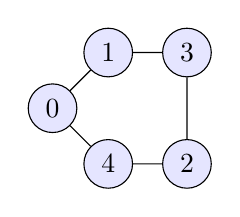
\begin{tikzpicture}[every node/.style={circle,fill=blue!10,draw,minimum size=0.4cm,node distance=1cm}]
                \node (1) {$1$};
                \node[below left of=1](0) {$0$};
                \node[below right of=0] (4) {$4$};
                \node[right of=4] (3) {$2$};
                \node[right of=1] (2) {$3$};
                \path[draw] (0) -- (1) -- (2) -- (3) -- (4) -- (0);
            \end{tikzpicture}                        
        \end{column}

    \end{columns}

    \begin{itemize}
        \item $\{0\}$ formulí $x=y$, tj. $(x=y)^{\mathcal G,\{0\}}=\{0\}$
        \item $\{1,4\}$ lze definovat pomocí $E(x,y)$
        \item $\{2,3\}$ formulí $\neg E(x,y)\land \neg x=y$
    \end{itemize}
    $\mathrm{Df}^1(\mathcal G,\{0\})$ je podalgebra $\underline{\mathcal P(V(\mathcal G))}$, tedy uzavřená na doplněk, sjednocení, průnik, obsahuje $\emptyset$ a $V(\mathcal G)$. Podalgebra generovaná $\{\{0\},\{1,4\},\{2,3\}\}$ už ale obsahuje všechny podmnožiny zachovávající automorfismus $h$. Dostáváme:
    \begin{align*}        
        \mathrm{Df}^1(\mathcal G,\{0\})=\{&\emptyset, \{0\}, \{1,4\}, \{2,3\}, \{0,1,4\}, \{0,2,3\}, \\ &\{1,4,2,3\}, \{0,1,2,3,4\}\}        
    \end{align*}
    
\end{frame}


\section{9.3 $\omega$-kategorické teorie}


\begin{frame}{$\omega$-kategorické teorie}

    \vspace{-8pt}
    \alert{Izomorfní spektrum} $T$ je počet modelů $T$ kardinality $\kappa$ až na $\simeq$.\\
    $T$ je \alert{$\kappa$-kategorická} pokud $I(\kappa,T)=1$, \alert{$\omega$-kategorická} má-li jediný spočetně nekonečný model až na izomorfismus.

    \vspace{-3pt}
    \myblock{
        \textbf{Tvrzení:}
        Teorie DeLO je $\omega$-kategorická.
    }
    \textbf{Důkaz:}
    Buďte $\A,\B$ spočetně nekonečné modely, $A=\{a_i\mid i\in\mathbb N\}$, $B=\{b_i\mid i\in\mathbb N\}$. Z hustoty najdeme indukcí $h_0\subseteq h_1\subseteq h_2\subseteq\dots$ prosté parciální fce z $A$ do $B$ zach. usp., $\{a_0,\dots,a_{n-1}\}\subseteq\dom h_n$, $\{b_0,\dots,b_{n-1}\}\subseteq\rng h_n$. Potom $\A\simeq\B$ via $h=\bigcup_{n\in\mathbb N}h_n$.
    \hfill\qedsymbol

    \myblock{
        \textbf{Důsledek:}
        Izomorfní spektrum teorie DeLO*:
        \vspace{-3pt}
        \begin{itemize}
            \item $I(\kappa,DeLO^*)=0$ pro $\kappa\in\mathbb{N}$
            \item $I(\omega,DeLO^*)=4$
        \end{itemize}      
        \vspace{-3pt}
        Spočetné modely až na izomorfismus jsou například:
        \vspace{-9pt}
        $$ 
        \mathbb Q=\langle \mathbb Q,\leq\rangle\simeq\mathbb Q\upharpoonright(0,1), \ \mathbb Q\upharpoonright(0,1], \ \mathbb Q \upharpoonright [0,1), \ \mathbb Q \upharpoonright [0,1]
        $$
        \vspace{-20pt}
    }
    \textbf{Důkaz:}
    Husté uspořádání nemůže být konečné. Izomorfismus zobrazí minimum na minimum a maximum na maximum.
    \hfill\qedsymbol

\end{frame}


\begin{frame}{$\omega$-kategorické kritérium kompletnosti}

    %\alert{$\omega$-kategoricita} je zeslabení pojmu \alert{kompletnosti}

    \myblock{
        \textbf{Věta:}
        Buď $T$ $\omega$-kategorická ve spočetném jazyce $L$. Je-li
        \begin{enumerate}[(i)]
            \item $L$ bez rovnosti, nebo
            \item $L$ s rovností a $T$ nemá konečné modely,
        \end{enumerate}
        potom je $T$ kompletní.
    }

    \textbf{Důkaz:}
    \alert{(i)} Důsledek L.-S. věty bez rovnosti říká, že každý model je elementárně ekvivalentní nějakému spočetně nekonečnému, ten je ale až na izomorfismus jediný.
    
    \alert{(ii)} Důsledek L.-S. věty s rovností podobně říká, že všechny nekonečné modely jsou elementárně ekvivalentní. Mohla by mít elementárně neekvivalentní konečné modely, to jsme ale zakázali. \hfill\qedsymbol

    \medskip

    \myblock{
        \textbf{Důsledek:}
        $\DeLO$, $\DeLO^+$, $\DeLO^-$, a $\DeLO^\pm$ jsou kompletní, jsou to všechny (navzájem neekvivalentní) kompletní jedn. extenze $DeLO^*$.
    }

    Analogické kritérium platí i pro kardinality $\kappa$ větší než $\omega$.

\end{frame}


\end{document}




\end{document}
\documentclass[handout]{beamer}
\usepackage{standalone}

\input{slides-header.tex}

\title{Dvanáctá přednáška}
\subtitle{NAIL062 Výroková a predikátová logika}
\author{Jakub Bulín (KTIML MFF UK)}
% \institute{KTIML MFF UK}
\date{Zimní semestr 2025}

\begin{document}

\documentclass{beamer}

\input{slides-header.tex}

\title{Dvanáctá přednáška}
\subtitle{NAIL062 Výroková a predikátová logika}
\author{Jakub Bulín (KTIML MFF UK)}
% \institute{KTIML MFF UK}
\date{Zimní semestr 2024}


\begin{document}


\maketitle


\begin{frame}{Dvanáctá přednáška}

    \textbf{Program}
        \begin{itemize}            
            \item axiomatizovatelnost
            \item rekurzivní axiomatizace a rozhodnutelnost
            \item aritmetické teorie
            \item nerozhodnutelnost predikátové logiky
            \item Gödelovy věty o neúplnosti
        \end{itemize}

    \textbf{Materiály}

        \href{https://github.com/jbulin-mff-uk/nail062/raw/main/lecture/lecture-notes/lecture-notes.pdf}{\alert{\textbf{Zápisky z přednášky}}}, Sekce 9.4 z Kapitoly 9, Kapitola 10

\end{frame}


\section{9.4 Axiomatizovatelnost}


\begin{frame}{Axiomatizovatelnost}
        
    Třída struktur $K\subseteq\M_L$ je:
    
    \begin{itemize}
        \item \alert{axiomatizovatelná}, existuje-li teorie $T$ taková, že $\M_L(T)=K$
        \item \alert{konečně}/\alert{otevřeně} axiomatiz., je-li ax. konečnou/otevřenou $T$
        \item teorie $T'$ je \alert{konečně}/\alert{otevřeně} axiomatizovatelná, platí-li to o třídě jejích modelů $K=\M_L(T')$
    \end{itemize}

    \textbf{Pozorování:} Je-li $K$ axiomatizovatelná, musí být uzavřená na $\equiv$.

    \medskip
    
    \myexample{
    Například, jak ukážeme:
    \begin{itemize}
        \item grafy a částečná uspořádání jsou konečně i otevřeně ax.
        \item tělesa jsou konečně, ale ne otevřeně axiomatizovatelná
        \item nekonečné grupy jsou axiomatizovatelné, ale ne konečně
        \item konečné grafy nejsou axiomatizovatelné
    \end{itemize}
    }

\end{frame}


\begin{frame}{Neaxiomatizovatelnost konečných modelů}

    \smallskip

    \myblock{
        \textbf{Věta:}
        Má-li $T$ libovolně velké konečné modely, má i nekonečný model. Potom není třída jejích konečných modelů axiomatizovatelná.
    }

    \textbf{Důkaz:}
    \alert{Je-li jazyk bez rovnosti,} vezmeme  kanonický model pro bezespornou větev v tablu z $T$ pro $\F\bot$ ($T$ je bezesporná).
    
    \alert{Je-li jazyk s rovností,} přidáme spočetně mnoho nových konst. symbolů $c_i$ a vezmeme extenzi: \myalertinline{
        $T'=T \cup \{\neg c_i = c_j \mid i\neq j\in\mathbb N\}$
    }

    \vspace{-2pt}

    Každá \alert{konečná část} $T'$ má model: buď $k$ největší, že $c_k$ je v této konečné části: lib. $\geq(k+1)$-prvkový model,21 interpretuj $c_0,\dots,c_k$ jako různé prvky.

    \vspace{-2pt}

    \alert{Věta o kompaktnosti} dává model $T'$, ten je nekonečný, redukt na původní jazyk (zapomenutí $c_i^\A$) je nekonečný model $T$.\hfill\qedsymbol

    \begin{itemize}
        \item např. \myexampleinline{konečné grafy} nejsou axiomatizovatelné
        \item \alert{nekonečné modely} teorie jsou vždy axiomatizovatelné, máme-li rovnost: stačí přidat \myalertinline{`existuje alespoň $n$ prvků'} pro vš. $n\in\mathbb N$
    \end{itemize}

\end{frame}


\begin{frame}{Konečná axiomatizovatelnost}
    
    \smallskip

    \myblock{
        \textbf{Věta (O konečné axiomatizovatelnosti):}
        $K\subseteq \M_L$ je konečně axiomatizovatelná, právě když $K$ i $\overline{K}=\M_L\setminus K$ jsou axiomatizovatelné.
    }

    \textbf{Důkaz:} \alert{\Large$\Rightarrow$}
    Je-li $K$ axiomatizovatelná \alert{sentencemi} $\varphi_1,\dots,\varphi_n$ (vezmi gen. uzávěry), potom $\neg(\varphi_1\land\varphi_2\land\dots\land\varphi_n)$ axiomatizuje $\overline{K}$.

    \alert{\Large$\Leftarrow$} Buď $K=\M(T)$ a $\overline{K}=\M(S)$. Potom  \alert{$T\cup S$ je sporná}, neboť:
    $$
    \M(T\cup S)=\M(T)\cap \M(S)=K\cap\overline{K}=\emptyset
    $$
    \alert{Věta o kompaktnosti} dává konečné $T'\subseteq T$ a $S'\subseteq S$ takové, že:
    $$
    \emptyset = \M(T'\cup S')=\M(T')\cap \M(S')
    $$
    Nyní si všimněme, že platí:
    $$
    \M(T)\subseteq \M(T')\subseteq \overline{\M(S')}\subseteq \overline{\M(S)}=\M(T)
    $$
    Tím jsme dokázali, že \alert{$M(T)=M(T')$}, neboli $T'$ je konečná axiomatizace $K$. \hfill\qedsymbol

\end{frame}


\begin{frame}{Tělesa charakteristiky 0 nejsou konečně axiomatizovatelná}

    Buď $T$ teorie těles. Těleso $\A=\langle A,+,-,0,\cdot,1 \rangle$ je
    \vspace{-6pt}
    \begin{itemize}
        \item \alert{charakteristiky $p$}, je-li $p$ nejmenší prvočíslo takové, že $\A\models p1=0$, kde $p1$ je term $1+1+\dots+1$ (s $p$ jedničkami),
        \item \alert{charakteristiky 0}, pokud není charakteristiky $p$ pro žádné $p$.
        \item Tělesa charakteristiky $p$ jsou konečně axiomatizovatelná: \myalertmath{\small
            $$
            T_p=T\cup \{p1=0\}
            $$
        }
        \item Tělesa char. 0 jsou axiomatizovatelná, ale ne konečně: \myalertmath{\small
            $$
            T_0=T\cup \{\neg\, p1=0\mid p\text{ prvočíslo}\}
            $$
        }
    \end{itemize}
    \myblock{\vspace{2pt}
        \textbf{Tvrzení:}
        Třída $K$ těles char. $0$ není konečně axiomatizovatelná.
        \vspace{2pt}
    }
    
    \textbf{Důkaz:}
    Stačí ukázat, že $\overline{K}$ (tělesa nenulové char. a netělesa) není axiomatizovatelná. \alert{Sporem: $\overline{K}=\M(S)$.} Potom  
    $S'=S\cup T_0$ má model, neboť každá konečná část má model: těleso charakteristiky větší než jakékoliv $p$ z axiomu $T_0$ tvaru $\neg\, p1=0$. Je-li $\A$ je model $S'$, potom $\A\in\M(S)=\overline{K}$. Zároveň ale $\A\in\M(T_0)=K$, spor.\hfill\qedsymbol

\end{frame}


\begin{frame}{Otevřená axiomatizovatelnost}

    \smallskip

    \myblock{\vspace{2pt}
        \textbf{Tvrzení:}
        Je-li $T$ otevřeně axiomatizovatelná, potom je každá podstruktura modelu $T$ také modelem $T$.
        \vspace{2pt}  
    }
    
    \textbf{Důkaz:}
    Buď $T'$ otevřená axiomatizace $T$, $\A$ model $T'$, $\B\subseteq\A$. Pro každou $\varphi\in T'$ platí $\B\models\varphi$ ($\varphi$ je otevřená), tedy i $\B\models T'$.  
    \hfill\qedsymbol

    \textbf{Poznámka:} Platí i obráceně, je-li každá podstruktura modelu také model, potom je otevřeně axiomatizovatelná. (Důkaz neuvedeme.)

    \begin{itemize}
        \item \myexampleinline{DeLO} není otevřeně axiomatizovatelná, např. žádná konečná podstruktura modelu DeLO není hustá
        \item \myexampleinline{teorie těles} není otevřeně axiomatizovatelná, podstruktura $\mathbb Z\subseteq\mathbb Q$ není těleso, nemá inverzní prvek k $2$ vůči násobení
        \item pro dané $n\in\mathbb N$ jsou \myexampleinline{nejvýše $n$-prvkové grupy} otevřeně axiomatizovatelné (i jejich podgrupy jsou nejvýše $n$-prvkové); k (otevřené) teorii grup stačí přidat: \myalertinline{
            $\bigvee_{1\leq i<j\leq n+1}x_i=x_j$
        }
    \end{itemize}

\end{frame}


\section{\sc Kapitola 10: Nerozhodnutelnost a neúplnost}


\begin{frame}{Nerozhodnutelnost a neúplnost}

    Jak lze s teoriemi pracovat algoritmicky?

    \medskip

    + zlatý hřeb přednášky: \alert{Gödelovy věty o neúplnosti} (1931)
    \begin{itemize}
        \item ukazují limity formálního přístupu
        \item zastavily program formalizace matematiky
        \item pojem \alert{algoritmu} budeme chápat jen intuitivně
        \item technické podrobnosti důkazů vynecháme
        
    \end{itemize}

    Typicky potřebujeme spočetný jazyk.
     
\end{frame}


\section{10.1 Rekurzivní axiomatizace a rozhodnutelnost}


\begin{frame}{Rekurzivní axiomatizace}

    \begin{itemize}
        \item v dokazování povolujeme nekonečné teorie, jak jsou zadané?
        \item pro ověření že daný důkaz (např. tablo, rezoluční zamítnutí) je korektní potřebujeme algoritmický přístup ke všem axiomům
        \item mohli bychom požadovat \alert{enumerátor} pro $T$, tj. algoritmus, který vypisuje axiomy z $T$, a každý axiom někdy vypíše
        \item ale kdyby byl v důkazu chybný axiom, nikdy bychom se to nedozvěděli: stále bychom čekali, zda ho enumerátor vypíše
        \item proto požadujeme silnější vlastnost:
    \end{itemize}

    \myblock{
        $T$ je \alert{rekurzivně axiomatizovaná}, pokud existuje algoritmus, který pro každou vstupní formuli $\varphi$ doběhne a odpoví, zda $\varphi\in T$.
    }

    (ekvivalentní enumerátoru vypisujícímu axiomy v lexikograf. pořadí)  

\end{frame}


\begin{frame}{Rozhodnutelnost}

    \vspace{-3pt}
    Můžeme v dané teorii \alert{`algoritmicky rozhodovat pravdu'}?

    \vspace{-3pt}
    \myblock{
        \begin{itemize}
            \item $T$ je \alert{rozhodnutelná}, pokud existuje algoritmus, který pro každou vstupní formuli $\varphi$ doběhne a odpoví, zda $T\models\varphi$,
            \item $T$ je \alert{částečně rozhodnutelná}, existuje-li algoritmus, který: %pro každou vstupní formuli:
            \begin{itemize}
                \item pokud $T\models\varphi$, doběhne a odpoví ``ano''
                \item pokud $T\not\models\varphi$, buď nedoběhne, nebo doběhne a odpoví ``ne''
            \end{itemize}
        \end{itemize}
    }

    
    \myblock{
        \textbf{Tvrzení:}
        Je-li $T$ je rekurzivně axiomatizovaná, potom:
                
        (i) $T$ je část. rozhod. \hfill (ii) je-li navíc kompletní, je rozhodnutelná
    }
    
    
    \textbf{Důkaz:} \alert{(i)} Algoritmus konstruuje systematické tablo z $T$ pro $\F\varphi$; stačí enumerátor pro $T$, nebo postupně generovat vš. sentence a testovat, jsou-li v $T$. Je-li $T\models\varphi$, konstrukce skončí, ověříme, že je tablo sporné. (Jinak skončit nemusí.)
    
    \vspace{-3pt}  
    \alert{(ii)}
    Víme, že buď $T\proves\varphi$ nebo $T\proves\neg\varphi$. Paralelně konstruujeme tablo pro $\F\varphi$ a pro $\T\varphi$ (důkaz a zamítnutí $\varphi$ z $T$). Jedna z konstrukcí po konečně mnoha krocích skončí.
    \hfill\qedsymbol


\end{frame}


\begin{frame}{Rekurzivně spočetná kompletace}

    \myblock{
        $T$ má \alert{rekurzivně spočetnou kompletaci}, je-li (nějaká) množina až na $\sim$ všech jednoduchých kompletních extenzí $T$ \alert{rekurzivně spočetná}, tj. existuje algoritmus, který pro vstup $(i,j)$ vypíše $i$-tý axiom $j$-té extenze (v nějakém uspořádání), nebo odpoví, že už neexistuje.
    }
     
    \myblock{
        \textbf{Tvrzení:}
        Je-li $T$ rekurzivně axiomatizovaná a má rekurzivně spočetnou kompletaci, potom je rozhodnutelná.
    }
        
    \textbf{Důkaz:}
    Buď $T\proves\varphi$, nebo existuje protipříklad $\A\not\models\varphi$, tj. kompl. jedn. extenze $T_i$, že $T_i\not\proves\varphi$. Kompletnost $T_i$ dává $T_i\proves\neg\varphi$. 
    
    Algoritmus paralelně konstruuje tablo důkaz $\varphi$ z $T$ a (postupně) tablo důkazy $\neg\varphi$ ze všech kompletních jedn. extenzí $T_1,T_2,\dots$. (Je-li jich nekonečně mnoho, uděláme \alert{dovetailing}: 1. krok 1. tabla, potom 2. krok 1., 1. krok 2., 3. krok 1., 2. krok 2., 1. krok 3., atd.)
    
    Alespoň jedno z tabel je sporné, můžeme předpokládat konečné, algoritmus ho po konečně mnoha krocích zkonstruuje.
    \hfill\qedsymbol

\end{frame}


\begin{frame}{Příklady}
    
    Následující teorie jsou rekurzivně axiomatizované a mají rekurzivně spočetnou kompletaci, tedy jsou rozhodnutelné:

    \myexample{
    \begin{enumerate}[(a)]
    \item Teorie čisté rovnosti
    \item Teorie unárního predikátu ($T=\emptyset$, $L=\langle U \rangle$ s rovností)
    \item Teorie hustých lineárních uspořádání DeLO*
    \item Teorie Booleových algeber (Alfred Tarski 1940),
    \item Teorie algebraicky uzavřených těles (Tarski 1949),
    \item Teorie komutativních grup (Wanda Szmielew 1955).
    \end{enumerate}
    }

\end{frame}


\begin{frame}{Rekurzivní axiomatizovatelnost}

    Kdy lze třídu struktur `efektivně (algoritmicky) popsat'?

    \myblock{
        $K\subseteq\M_L$ je \alert{rek. axiomatizovatelná}, pokud existuje rek. axiomatizovaná $T$, že $K=M_L(T)$. $T'$ je \alert{rek. axiomatizovatelná}, platí-li to pro třídu jejích modelů (tj. je-li ekvivalentní rek. axiomatizované teorii).
    }

    (podobně lze definovat \alert{rek. spočetnou axiomatizovatelnost})

    \myblock{
        \textbf{Tvrzení:}
        Je-li $\A$ konečná struktura v konečném jazyce s rovností, potom je teorie $\Th(\A)$ rekurzivně axiomatizovatelná.
    }
        
    (z toho plyne i rozhodnutelnost $\Th(\A)$, ale $\A\models\varphi$ lze ověřit přímo)

    \textbf{Důkaz:}
    Buď $A=\{a_1,\dots,a_n\}$. $\Th(\A)$ axiomatizujeme sentencí ``existuje právě $n$ prvků $a_1,\dots,a_n$ splňujících právě ty \alert{základní vztahy} o funkčních hodnotách a relacích, které platí v $\A$''.
    
    Např. je-li $f^\A(a_4, a_2)=a_{17}$, přidej atom. formuli $f(x_{a_4},x_{a_2})=x_{a_{17}}$, je-li $(a_3,a_3,a_1)\notin R^\A$ přidej $\neg R(x_{a_3},x_{a_3},x_{a_1})$.\hfill\qedsymbol

\end{frame}


\begin{frame}{Příklady}

    Pro následující struktury je $\Th(\A)$ rekurzivně axiomatizovatelná:

    \myexample{
        \begin{itemize}
            \item $\langle\mathbb Z,\leq\rangle$, jde o tzv. teorii \alert{diskrétních lineárních uspořádání}        
            \item $\langle\mathbb Q,\leq\rangle$, jde o teorii DeLO
            \item $\langle\mathbb N,S,0\rangle$, teorie \alert{následníka s nulou}
            \item $\langle\mathbb N,S,+,0\rangle$, \alert{Presburgerova aritmetika}
            \item $\langle\mathbb R,+,-,\cdot,0,1\rangle$, teorie \alert{reálně uzavřených těles}, znamená že lze algoritmicky rozhodovat Euklid. geometrii (Tarski, 1949)
            \item $\langle \mathbb C,+,-,\cdot,0,1 \rangle$, teorie \alert{algebraicky uzavřených těles char. 0}
        \end{itemize}
    }

    \medskip

    \myblock{
        \textbf{Důsledek:}
        Pro struktury výše platí, že $\Th(\A)$ je rozhodnutelná.
    }
    \textbf{Důkaz:} $\Th(\A)$ je vždy kompletní.

    \myexample{
        Teorie \alert{standardního modelu aritmetiky} $\underline{\mathbb N}=\langle\mathbb N,S,+,\cdot,0,\leq\rangle$ ale \alert{není} rekurzivně axiomatizovatelná (viz První Gödelova věta o neúplnosti).
    }

\end{frame}


\section{10.2 Aritmetika}


\begin{frame}{Aritmetika}

    \begin{itemize}
        \item přirozená čísla hrají důležitou roli v matematice i v aplikacích
        \item \alert{jazyk aritmetiky} je $L=\langle S,+,\cdot,0,\leq\rangle$ s rovností
        \item \alert{standardní model aritmetiky}  $\underline{\mathbb N}=\langle\mathbb N,S,+,\cdot,0,\leq\rangle$ nemá rekurzivně axiomatizovatelnou teorii (První věta o neúplnosti)
        \item proto používáme rekurzivně axiomatizované teorie, které vlastnosti $\underline{\mathbb N}$ popisují částečně; říkáme jim \alert{aritmetiky}       
        \item představíme dvě: \alert{Robinsonovu} $Q$ a \alert{Peanovu} $PA$
    \end{itemize}

\end{frame}


\begin{frame}{Robinsonova aritmetika $Q$}    

    \myblockamsmath{ 
        \vspace{-12pt}       
        \begin{align*}
            &\neg S(x) = 0& &x\cdot 0=0\\
            &S(x)=S(y)\rightarrow x=y& &x\cdot S(y)=x\cdot y+x\\
            &x+0=x& &\neg x=0 \rightarrow (\exists y)(x=S(y))\\
            &x+S(y)=S(x+y)& &x\le y \leftrightarrow (\exists z)(z+x=y)\qquad
        \end{align*}
    }
    
    \begin{itemize}
        \item velmi slabá, nelze v ní dokázat např. komutativitu ani asociativitu $+$ či $\cdot$, nebo tranzitivitu $\leq$
        \item ale lze dokázat všechna \alert{existenční tvrzení o numerálech} pravdivá v $\underline{\mathbb N}$, tj. formule v PNF, jen $\exists$, za volné proměnné substituujeme \alert{numerály} $\underline{n}=S(\dots S(0)\dots)$
        \item např. pro \myexampleinline{
            $\varphi(x,y)=(\exists z)(x+z=y)$
         } je $Q\proves\varphi(\underline{1},\underline{2})$
    \end{itemize}

    \medskip
    
    \myblock{
        \textbf{Tvrzení:}
        Je-li $\varphi(x_1,\dots,x_n)$ existenční formule, $a_1,\dots,a_n\in\mathbb N$, pak
        $Q\proves\varphi(x_1/\underline{a_1},\dots,x_n/\underline{a_n})$ právě když $\underline{\mathbb{N}}\models \varphi[e(x_1/a_1,\dots,x_n/a_n)]
        $
    }

    (Důkaz vynecháme.)

\end{frame}


\begin{frame}{Peanova aritmetika $PA$}    

    \myblock{
        Extenze $Q$ o \alert{schéma indukce}, tj. pro každou $L$-formuli $\varphi(x,\overline{y})$:
        \vspace{-6pt}
        $$
        (\varphi(0,\overline{y}) \land (\forall x)(\varphi(x,\overline{y})\limplies \varphi(S(x),\overline{y}))) \limplies (\forall x)\varphi(x,\overline{y})
        $$
        \vspace{-21pt}
    }

    \begin{itemize}
        \item mnohem lepší aproximace $\Th(\underline{\mathbb N})$
        \item dokáže `základní' vlastnosti (např. komut. a asociativitu $+$) \item stále ale existují sentence platné v $\underline{\mathbb N}$ ale nezávislé v $PA$\\(opět dokážeme v První větě o neúplnosti)
    \end{itemize}

    \bigskip

    \textbf{Poznámka:} strukturu $\underline{\mathbb N}$ lze axiomatizovat (až na $\simeq$) v predikátové logice \alert{2. řádu}, extenzí $PA$ o tzv. \alert{axiom indukce}:
    $$
    (\forall X)((X(0) \land (\forall x)(X(x) \limplies X(S(x)))) \limplies (\forall x)X(x))
    $$

    \begin{itemize}
        \item $X$ reprezentuje (libovolnou) podmnožinu modelu
        \item použijeme na množinu všech následníků 0
        \item každý prvek je následník 0 $\Rightarrow$ izomorfismus s $\underline{\mathbb N}$
    \end{itemize}

\end{frame}


\section{10.3 Nerozhodnutelnost predikátové logiky}


\begin{frame}{Nerozhodnutelnost predikátové logiky}
    
    \myblock{
        \textbf{Věta (O nerozhodnutelnosti predikátové logiky):}
        Neexistuje algoritmus, který pro vstupní formuli $\varphi$ rozhodne, zda je logicky platná.
    }

    \begin{itemize}
        \item tj. zda je formule $\varphi$ [v lib. jazyce 1. řádu] tautologie ($\models\varphi$)
        \item neboli $T=\emptyset$ není rozhodnutelná 
    \end{itemize}

    Nemáme formalismus pro algoritmy (Turingovy stroje), dokážeme redukcí na jiný nerozhodnutelný problém: \alert{\href{https://en.wikipedia.org/wiki/Hilbert\%27s_problems}{Hilbertův 10. problém}}

    \bigskip

    \myalert{
    \begin{quote}
        ``Najděte algoritmus, který po konečně mnoha krocích určí, zda daná diofantická rovnice s libovolným počtem proměnných a
        celočíselnými koeficienty má celočíselné řešení.''
    \end{quote}
    }

    \medskip

    \alert{diofantická rovnice}: $p(x_1,\dots,x_n)=0$, kde $p$ je celočíselný polynom


    ukážeme, že existuje \alert{redukce} `těžkého' Hilbertova 10. problému na náš problém, tedy i náš problém je `těžký'
    
\end{frame}


\begin{frame}{Nerozhodnutelnost Hilbertova desátého problému}

    \myblock{
        \textbf{Věta (Matiyasevich 1970):}    
        Problém existence celočíselného řešení dané diofantické rovnice s celočís. koeficienty je nerozhodnutelný.
    }

    (Důkaz neuvedeme.)

    \medskip

    \myblock{
        \textbf{Důsledek:}
        Neexistuje algoritmus rozhodující, mají-li dané polynomy $p(x_1,\dots,x_n),q(x_1,\dots,x_n)$ s \alert{přiroz.} koeficienty \alert{přirozené řešení}, tj.
        \vspace{-6pt}
        $$
        \underline{\mathbb N}\models(\exists x_1)\dots(\exists x_n)\ p(x_1,\dots,x_n)=q(x_1,\dots,x_n)
        $$
        \vspace{-16pt}
    }
    
    \textbf{Důkaz:} \alert{\href{https://en.wikipedia.org/wiki/Lagrange\%27s_four-square_theorem}{Lagrangeova věta o čtyřech čtvercích}} říká, že každé přirozené číslo lze vyjádřit jako součet čtyř čtverců (celých čísel). Naopak, každé celé číslo je rozdíl dvou přirozených. Diofantickou rovnici lze tedy transformovat na rovnici z důsledku, a naopak.\hfill\qedsymbol

\end{frame}


\begin{frame}{Důkaz nerozhodnutelnosti predikátové logiky}

    Uvažme $\varphi$ tvaru $(\exists x_1)\dots(\exists x_n)\ p(x_1,\dots,x_n)=q(x_1,\dots,x_n)$ 
    kde $p$ a $q$ jsou přirozené polynomy. Dle Tvrzení o Robinsonově aritmetice:
    $$
    \underline{\mathbb N}\models \varphi\ \Leftrightarrow\  Q\proves \varphi
    $$

    Buď $\psi_Q$ konjunkce (gen. uzávěrů) axiomů $Q$ (je konečná). Zřejmě: 
    $$
    \alert{Q\proves\varphi}\ \Leftrightarrow\ \psi_Q\proves\varphi\ \Leftrightarrow\ \alert{\proves\psi_Q\limplies\varphi}
    $$
    Dle Věty o úplnosti je to ale ekvivalentní \alert{$\models\psi_Q\limplies\varphi$}. Dostáváme:
    $$
    \underline{\mathbb N}\models \varphi\ \Leftrightarrow\ \models \psi_Q\limplies\varphi
    $$
    \alert{Sporem:} Pokud bychom měli algoritmus rozhodující logickou platnost, mohli bychom rozhodovat i existenci přirozeného řešení rovnice $p(x_1,\dots,x_n)=q(x_1,\dots,x_n)$, tj. Hilbertův 10. problém.\hfill\qedsymbol


\end{frame}


\section{10.4 Gödelovy věty}


\begin{frame}{První věta o neúplnosti + důsledek o nekompletnosti}

    \myblock{
        \textbf{Věta (Gödel 1931):}
        Je-li $T$ bezesporná rekurzivně axiomatizovaná extenze Robinsonovy aritmetiky, potom existuje sentence, která je pravdivá v~$\underline{\mathbb N}$, ale není dokazatelná v $T$.
    }

    \begin{itemize}
        \item vlastnosti aritmetiky přir. čísel nelze `rozumně', efektivně popsat (v logice 1. řádu), takový popis je nutně `neúplný'
        \item \alert{pravdivost} je ve standardním modelu $\underline{\mathbb N}$ zatímco \alert{dokazatelnost} v $T$ (samozřejmě pravdivá v $T$ je v $T$ i dokazatelná)
        \item \alert{bezespornost} nutná (sporná teorie dokáže vše)
        \item bez \alert{rekurzivní axiomatizovatelnosti} by teorie nebyla `užitečná'
        \item extenze $Q$ znamená `základní aritmetická síla' (různé varianty předpokladu; nelze-li zakódovat přir. čísla s $+,\cdot$ je moc `slabá'
    \end{itemize}    

    \myblock{
        \textbf{Důsledek:}
        Splňuje-li teorie $T$ předpoklady První věty o neúplnosti a je-li navíc $\underline{\mathbb N}$ modelem $T$, potom $T$ není kompletní.
    }
    
    \textbf{Důkaz:}
        Vezměme Gödelovu sentenci $\varphi$ ($\underline{\mathbb N}\models\varphi$, $T\not\proves\varphi$). Je-li $T$ kompletní, víme $T\proves\neg\varphi$, z korektnosti $T\models\neg\varphi$, tedy $\underline{\mathbb N}\models\neg\varphi$.
    \hfill\qedsymbol    

\end{frame}


\begin{frame}{O důkazu}

    \begin{itemize}
        \item Gödelova sentence formalizuje \alert{``Nejsem dokazatelná v $T$''}
        \item převratná důkazová technika, dva hlavní principy:
        \item \alert{aritmetizace syntaxe}, zakódování sentencí a jejich dokazatelnosti do přirozených čísel
        \item \alert{self-reference}, sentence `mluví sama o sobě' (o svém kódu)
        \item všechny technické detaily vynecháme, viz např. V. Švejdar: \emph{Logika -- neúplnost, složitost a nutnost}, Academia 2002
    \end{itemize}
    
\end{frame}


\begin{frame}{Aritmetizace syntaxe a dokazatelnosti}
    
    \begin{itemize}
        \item \alert{Gödelovo číslování} `rozumně' kóduje konečné syntaktické objekty (termy, formule, tablo důkazy) do $\mathbb N$: lze algoritmicky [de-]kódovat, simulovat `manipulaci' s objekty na jejich kódech
        \item pro $\varphi$ bude \alert{$\lceil\varphi\rceil$} příslušný kód, \alert{$\underline{\varphi}$} odpovídající $\lceil\varphi\rceil$-tý numerál
        \item pro danou $T$ máme binární relaci $\MyProof_T\subseteq\mathbb N^2$ definovanou
        \hspace{-1cm}\myalertinline{
            $(n,m)\in\MyProof_T$ $\Leftrightarrow$
        $n=\lceil\varphi\rceil$, $m=\lceil\tau\rceil$, $\tau$ je tablo důkaz $\varphi$ z $T$
        }
        \item je-li $T$ rek. axiomatizovaná, je relace $\MyProof_T\subseteq\mathbb N^2$ \alert{rekurzivní} (lze algoritmicky ověřit korektnost tabla, tj. $(n,m)\in\MyProof_T$)
        \item klíčovou technickou částí důkazu První věty je fakt, že relaci $\MyProof_T$ lze \alert{reprezentovat} predikátem v Robinsonově aritmetice

    \end{itemize}    

\end{frame}


\begin{frame}{Predikát dokazatelnosti}

    \myblock{
        \textbf{Tvrzení:}
        Je-li $T$ rekurzivně axiomatizovaná extenze Robinsonovy aritmetiky, potom existuje formule $\Prf_T(x,y)$ v jazyce aritmetiky, která \alert{reprezentuje} relaci $\MyProof_T$, tj. pro každá $n,m\in\mathbb N$:
    \begin{itemize}
        \item je-li $(n,m)\in\MyProof_T$, potom $Q\proves\Prf_T(\underline{n},\underline{m})$
        \item jinak $Q\proves\neg\Prf_T(\underline{n},\underline{m})$
    \end{itemize} 
    }

    (Důkaz vynecháme!)

    \begin{itemize}
        \item formule \myalertinline{
            $\Prf_T(x,y)$
            } vyjadřuje \alert{``$y$ je důkaz $x$ v $T$''}
        \item formule \myalertinline{
            $(\exists y)\Prf_T(x,y)$
            } znamená \alert{``$x$ je dokazatelná v $T$''}
        \item svědek poskytuje kód tablo důkazu, a $\underline{\mathbb N}$ splňuje $Q$, proto:
    \end{itemize}

    \myblock{
    \textbf{Pozorování:} $T\proves\varphi$ právě když $\underline{\mathbb N}\models (\exists y)\Prf_T(\underline{\varphi},y)$.  
    }
    
    Budeme potřebovat následující důsledek (také bez důkazu):
    
    \myblock{
    \textbf{Důsledek:}
        Je-li $T\proves\varphi$, potom $T\proves (\exists y)\Prf_T(\underline{\varphi},y)$.
    }
    
\end{frame}


\begin{frame}[fragile]{Self-reference}

    \vspace{-6pt}
    vyjádřili jsme \myalertinline{
        $\varphi$ je dokazatelná
    } ale chceme \myalertinline{já nejsem dokazatelná}
    
    přirozené jazyky mají self-referenci:
    \myexampleinline{\texttt{Tato věta má 22 znaků.}};  
    formální systémy obvykle ne, umožňují ale \alert{přímou referenci} (mluvit o posloupnostech symbolů):
    
    \medskip

    \myexample{
        \texttt{Následující věta má 29 znaků. "Následující věta má 29 znaků."}
    }

    \medskip

    zde není žádná self-reference, pomůžeme si proto trikem \alert{zdvojení}:
    
    \medskip

    \myexample{   
        \texttt{Následující věta zapsaná jednou a ještě jednou v uvozovkách má 149 znaků. "Následující věta zapsaná jednou a ještě jednou v uvozovkách má 149 znaků."}
    }  

    \medskip

    \myalertinline{přímou referencí a zdvojením tedy získáme self-referenci}; podobně program v C, který vypíše svůj kód (34 je ASCII kód uvozovek): 

    \vspace{-6pt}
    {\small
    \begin{verbatim}
main(){char *c="main(){char *c=%c%s%c; printf(c,34,c,34);}"; 
printf(c,34,c,34);}  
    \end{verbatim}
    }    

\end{frame}


\begin{frame}{Věta o pevném bodě}
    
    \myblock{
        \textbf{Věta:}
        Je-li $T$ extenzí Robinsonovy aritmetiky, potom pro každou formuli $\varphi(x)$ (v jazyce teorie $T$) existuje sentence $\psi$ taková, že: 

        \vspace{-9pt}
        $$
        T\proves \psi \liff \varphi(\underline{\psi})
        $$
    }

    \begin{itemize}
        \item také ``diagonalizační lemma'' nebo ``self-referenční'' lemma
        \item $\psi$ je \alert{self-referenční}, říká o sobě: \myalertinline{``já splňuji vlastnost $\varphi$''}
        \item v důkazu První věty bude $\varphi(x)$ formule $\neg(\exists y)\Prf_T(x,y)$
        %\item důkaz využívá diagonalizační argument (jako Holičův paradox)
        \item všimněte si, jak se v důkazu použije přímá reference a zdvojení
    \end{itemize}

    \textbf{Důkaz (myšlenka):} \alert{Zdvojující funkce} $d\colon\mathbb N\to\mathbb N$ dekóduje vstup $n$ jako $\varphi(x)$, dosadí numerál $\underline{n}$, znovu zakóduje: pro vš. $\chi(x)$ platí:
    $$
    \alert{d(\lceil \chi(x)\rceil)=\lceil\chi(\underline{\chi(x)})\rceil}
    $$
    S využitím $T$ extenze $Q$ se dokáže, že $d$ je v $T$ \alert{reprezentovatelná}. \myexampleinline{Pro jednoduchost ať ji reprezentuje term}, označíme ho také $d$ (ale ve skutečnosti je to složitá formule).
    
\end{frame}


\begin{frame}{Pokračování důkazu}

    Tedy $Q$, proto i $T$, dokazuje \alert{o numerálech}, že $d$ opravdu `zdvojuje':
    $$
    T\proves d(\underline{\chi(x)})=\underline{\chi(\underline{\chi(x)})}
    $$
        
    Hledaná self-referenční sentence $\psi$ je sentence:

        \myalertmath{
        $$
        \varphi(d(\underline{\varphi(d(x))}))
        $$
        }

    \bigskip

    Chceme dokázat, že $T\proves \psi \liff \varphi(\underline{\psi})$, neboli:
    $$
    T \proves \varphi(\alert{d(\underline{\varphi(d(x))})})\liff\varphi(\alert{\underline{\varphi(d(\underline{\varphi(d(x))}))}})
    $$
    
    K~tomu stačí \myalertinline{
        $T \proves d(\underline{\varphi(d(x))})=\underline{\varphi(d(\underline{\varphi(d(x))}))}$
    } což máme z reprezentovatelnosti $d$, kde $\chi(x)$ je $\varphi(d(x))$.\hfill\qedsymbol

    {\footnotesize
    $\psi$ tedy říká: >>Následující věta zapsaná jednou a ještě jednou v uvozovkách má vlastnost $\varphi$. ``Následující věta zapsaná jednou a ještě jednou v uvozovkách má vlastnost $\varphi$.''<< kde v uvozovkách znamená numerál kódu (přímá reference)
    }

\end{frame}


\begin{frame}{Nedefinovatelnost pravdy}

    \myblock{
        \textbf{Věta:}
        V žádném bezesporném rozšíření Robinsonovy aritmetiky nemůže existovat definice pravdy.
    }
    \vspace{-12pt}
    \begin{itemize}
        \item \alert{definice pravdy} v aritmetické teorii $T$ je formule $\tau(x)$ taková, že pro každou sentenci $\psi$ platí: 
        \myalertinline{
            $T\proves\psi\liff\tau(\underline{\psi})$
        }
        \item kdyby existovala, místo dokazování by stačilo spočíst kód $\lceil \psi\rceil$, dosadit numerál $\underline{\psi}$ do $\tau$, a vyhodnotit
        \item rozcvička pro důkaz Gödelovy První věty o neúplnosti
        \item důkaz užívá \alert{Paradox lháře}, vyjádříme \myalertinline{``Nejsem pravdivá v $T$''}
        \item důkaz První věty užívá stejný trik s ``Nejsem dokazatelná v $T$''
    \end{itemize}
    \vspace{-3pt}
    \textbf{Důkaz:} Sporem, ať existuje definice pravdy $\tau(x)$. Z Věty o pevném bodě kde $\varphi(x)$ je $\neg\tau(x)$ dostáváme sentenci $\psi$ takovou, že:
    $$
    T\proves\psi\liff\neg\tau(\underline{\psi})
    $$
    Protože $\tau(x)$ je definice pravdy, platí ale i $T\proves\psi\liff\tau(\underline{\psi})$, tedy i $T\proves\tau(\underline{\psi})\liff\neg\tau(\underline{\psi})$. To by ale znamenalo, že $T$ je sporná.
    \hfill\qedsymbol
    
\end{frame}


\begin{frame}{Důkaz První věty o neúplnosti}

    $T$ bezesp. rek. ax. ext. $Q$. Gödelovu sentenci ($\underline{\mathbb N}\models\psi_T,T\not\proves\psi_T$) získáme z Věty o pevném bodě kde $\varphi(x)$ je \alert{$\neg(\exists y)\Prf_T(x,y)$}:

    \myalertmath{
    $$
    T\proves\psi_T\liff\neg(\exists y)\Prf_T(\underline{\psi_T},y)
    $$
    }

    Tedy $\psi_T$ je v $T$ ekvivalentní ``$\psi_T$ není dokazatelná v $T$''. Ekvivalence platí i v $\underline{\mathbb N}$ (z konstrukce, protože $\underline{\mathbb N}$ splňuje $Q$), a spolu s ekvivalencí z Pozorování o predikátu dokazatelnosti:    
    $$
    \alert{\underline{\mathbb N}\models\psi_T}\ \Leftrightarrow\ 
    \underline{\mathbb N}\models\neg(\exists y)\Prf_T(\underline{\psi_T},y)\ \Leftrightarrow\ \alert{T\not\proves\psi_T}
    $$    

    Stačí tedy ukázat nedokazatelnost $\psi_T$ v $T$. \alert{Sporem: ať $T\proves\psi_T$. }
    
    \begin{itemize}
        \item Self-reference: $T\proves\neg(\exists y)\Prf_T(\underline{\psi_T},y)$
        \item Důsledek o predikátu dokazatelnosti: $T\proves (\exists y)\Prf_T(\underline{\psi_T},y)$
    \end{itemize}
    To by ale znamenalo, že $T$ je sporná.\hfill\qedsymbol
    
\end{frame}


\begin{frame}{Důsledky a zesílení}
    
    \myblock{
        \textbf{Důsledek (už byl):}
        Je-li $T$ rekurzivně axiomatizovaná extenze Robinsonovy aritmetiky a je-li $\underline{\mathbb N}$ model $T$, potom $T$ není kompletní.        
    }
    
    \textbf{Důkaz:}
        $T$ není sporná, tedy splňuje předpoklady První věty. Víme, že G. sentence splňuje $\underline{\mathbb N}\models\psi_T$ a $T\not\proves\psi_T$. Je-li $T$ kompletní, máme $T\proves\neg\psi_T$, z korektnosti $T\models\neg\psi_T$, tj. $\underline{\mathbb N}\models\neg\psi_T$, spor.
    \hfill\qedsymbol
    
    \medskip

    \myblock{\textbf{Důsledek:}
    Teorie $\Th(\underline{\mathbb N})$ není rekurzivně axiomatizovatelná.    
    }

    \textbf{Důkaz:}
    $\Th(\underline{\mathbb N})$ je extenze $Q$, platí v $\underline{\mathbb N}$. Kdyby byla rekurzivně axiomatizovatelná, podle Důsledku by [její rekurzivní axiomatizace] nebyla kompletní, ale je.
    \hfill\qedsymbol

    \medskip

    Zesílení První věty: předpoklad $\underline{\mathbb N}\models T$ v Důsledku je nadbytečný.

    \myblock{\textbf{Věta (Rosserův trik, 1936):}
    V bezesporné rekurzivně axiomatizované extenzi Robinsonovy aritmetiky existuje nezávislá sentence.  
    }

    (Bez důkazu.)

\end{frame}


\begin{frame}{Gödelova Druhá věta o neúplnosti}
    
    \myalert{
        Efektivně daná, dostatečně bohatá $T$ nedokáže svou bezespornost.
    }

    \begin{itemize}
        \item bezespornost vyjádří sentence \alert{$\Con_T$}:\hfill \myalertinline{\small
            $\neg(\exists y)\Prf_T(\underline{0=S(0)},y)$
        }  
        \item všimněte si: $\underline{\mathbb N}\models\Con_T$ $\Leftrightarrow$ $T\not\proves 0=S(0)$
        \item tj. $\Con_T$ opravdu vyjadřuje, že \alert{``$T$ je bezesporná''}
    \end{itemize}

    \bigskip
    
    \myblock{\textbf{Věta (Gödel, 1931):} Je-li $T$ bezesporná rekurzivně axiomatizovaná extenze $PA$, potom $\Con_T$ není dokazatelná v $T$.
    }

    \medskip

    \begin{itemize}
        \item všimněte si: \alert{$\Con_T$ je pravdivá v $\underline{\mathbb N}$} (neboť $T$ je bezesporná)
        \item není třeba plná síla $PA$, stačí slabší předpoklad
        \item ukážeme si hlavní myšlenku důkazu
    \end{itemize}
    
\end{frame}


\begin{frame}{Myšlenka důkazu}

    Gödelova sentence $\psi_T$ vyjadřuje: \myalertinline{``Nejsem dokazatelná v $T$.''}
    
    V důkazu První věty o neúplnosti jsme ukázali:

    \myalert{
        ``Pokud je $T$ bezesporná, potom $\psi_T$ není dokazatelná v $T$.''
    }
    
    Z toho jednak plyne, že $T\not\proves\psi_T$, neboť $T$ bezesporná je. 
    
    Na druhou stranu to lze formulovat jako: \myalertinline{``Platí $\Con_T\to \psi_T$.''}
    
    Je-li $T$ extenze Peanovy aritmetiky, lze důkaz tohoto tvrzení zformalizovat v rámci teorie $T$, tedy ukázat, že:
    $$
    \alert{ T\proves\Con_T\to\psi_T}
    $$
    Kdyby platilo $T\proves\Con_T$, dostali bychom i $T\proves\psi_T$, což je spor.
    \hfill\qedsymbol

\end{frame}


\begin{frame}{Důsledky}    

    \myblock{\textbf{Důsledek:}
        $PA$ má model, ve kterém platí $(\exists y)\Prf_{PA}(\underline{0=S(0)},y)$.
    }

    \textbf{Důkaz:}
        Sentence $\Con_{PA}$ není dokazatelná, tedy ani pravdivá v $PA$. Platí ale v $\underline{\mathbb N}$ (neboť $PA$ je bezesporná), což znamená, že je $\Con_{PA}$ nezávislá v $PA$. V nějakém modelu tedy musí platit její negace, která je ekvivalentní $(\exists y)\Prf_{PA}(\underline{0=S(0)},y)$.            
    \hfill\qedsymbol

    \textbf{Poznámka:} Musí to být nestandardní model $PA$, svědek \alert{nestandardní} prvek (není hodnotou žádného numerálu).

    \bigskip

    \myblock{\textbf{Důsledek:}
        $PA$ má bezespornou rekurzivně axiomatizovanou extenzi, která ``dokazuje svou spornost'', tj. $T\proves \neg \Con_T$.
    }

    \textbf{Důkaz:}
    $T=PA \cup \{\neg \Con_{PA}\}$ je \alert{bezesporná}, neboť $PA\not\proves\Con_{PA}$. Také triviálně $T\proves\neg\Con_{PA}$, tj. $T$ `dokazuje spornost' $PA$. Protože $PA\subseteq T$, platí i $T\proves\neg\Con_T$.
    \hfill\qedsymbol

    \textbf{Poznámka:} $\underline{\mathbb{N}}$ nemůže být modelem $T$.
    
\end{frame}


\begin{frame}{Bezespornost ZFC}

    Formalizace matematiky je založena na \href{https://en.wikipedia.org/wiki/Zermelo\%E2\%80\%93Fraenkel_set_theory}{\alert{Zermelově–Fraenkelově teorii množin s axiomem výběru (ZFC)}}. Formálně vzato to není extenze $PA$, ale můžeme v ní Peanovu aritmetiku `interpretovat'.

    \myblock{\textbf{Důsledek:}
        Je-li ZFC bezesporná, není $\Con_{ZFC}$ v ZFC dokazatelná.
    }

    Pokud by tedy někdo v rámci ZFC dokázal, že je ZFC bezesporná, znamenalo by to, že je ZFC sporná.    

\end{frame}


\end{document}





\end{document}

\end{document}